\documentclass[twoside]{book}

% Packages required by doxygen
\usepackage{fixltx2e}
\usepackage{calc}
\usepackage{doxygen}
\usepackage[export]{adjustbox} % also loads graphicx
\usepackage{graphicx}
\usepackage[utf8]{inputenc}
\usepackage{makeidx}
\usepackage{multicol}
\usepackage{multirow}
\PassOptionsToPackage{warn}{textcomp}
\usepackage{textcomp}
\usepackage[nointegrals]{wasysym}
\usepackage[table]{xcolor}

% Font selection
\usepackage[T1]{fontenc}
\usepackage[scaled=.90]{helvet}
\usepackage{courier}
\usepackage{amssymb}
\usepackage{sectsty}
\renewcommand{\familydefault}{\sfdefault}
\allsectionsfont{%
  \fontseries{bc}\selectfont%
  \color{darkgray}%
}
\renewcommand{\DoxyLabelFont}{%
  \fontseries{bc}\selectfont%
  \color{darkgray}%
}
\newcommand{\+}{\discretionary{\mbox{\scriptsize$\hookleftarrow$}}{}{}}

% Page & text layout
\usepackage{geometry}
\geometry{%
  a4paper,%
  top=2.5cm,%
  bottom=2.5cm,%
  left=2.5cm,%
  right=2.5cm%
}
\tolerance=750
\hfuzz=15pt
\hbadness=750
\setlength{\emergencystretch}{15pt}
\setlength{\parindent}{0cm}
\setlength{\parskip}{3ex plus 2ex minus 2ex}
\makeatletter
\renewcommand{\paragraph}{%
  \@startsection{paragraph}{4}{0ex}{-1.0ex}{1.0ex}{%
    \normalfont\normalsize\bfseries\SS@parafont%
  }%
}
\renewcommand{\subparagraph}{%
  \@startsection{subparagraph}{5}{0ex}{-1.0ex}{1.0ex}{%
    \normalfont\normalsize\bfseries\SS@subparafont%
  }%
}
\makeatother

% Headers & footers
\usepackage{fancyhdr}
\pagestyle{fancyplain}
\fancyhead[LE]{\fancyplain{}{\bfseries\thepage}}
\fancyhead[CE]{\fancyplain{}{}}
\fancyhead[RE]{\fancyplain{}{\bfseries\leftmark}}
\fancyhead[LO]{\fancyplain{}{\bfseries\rightmark}}
\fancyhead[CO]{\fancyplain{}{}}
\fancyhead[RO]{\fancyplain{}{\bfseries\thepage}}
\fancyfoot[LE]{\fancyplain{}{}}
\fancyfoot[CE]{\fancyplain{}{}}
\fancyfoot[RE]{\fancyplain{}{\bfseries\scriptsize Generated by Doxygen }}
\fancyfoot[LO]{\fancyplain{}{\bfseries\scriptsize Generated by Doxygen }}
\fancyfoot[CO]{\fancyplain{}{}}
\fancyfoot[RO]{\fancyplain{}{}}
\renewcommand{\footrulewidth}{0.4pt}
\renewcommand{\chaptermark}[1]{%
  \markboth{#1}{}%
}
\renewcommand{\sectionmark}[1]{%
  \markright{\thesection\ #1}%
}

% Indices & bibliography
\usepackage{natbib}
\usepackage[titles]{tocloft}
\setcounter{tocdepth}{3}
\setcounter{secnumdepth}{5}
\makeindex

% Hyperlinks (required, but should be loaded last)
\usepackage{ifpdf}
\ifpdf
  \usepackage[pdftex,pagebackref=true]{hyperref}
\else
  \usepackage[ps2pdf,pagebackref=true]{hyperref}
\fi
\hypersetup{%
  colorlinks=true,%
  linkcolor=blue,%
  citecolor=blue,%
  unicode%
}

% Custom commands
\newcommand{\clearemptydoublepage}{%
  \newpage{\pagestyle{empty}\cleardoublepage}%
}

\usepackage{caption}
\captionsetup{labelsep=space,justification=centering,font={bf},singlelinecheck=off,skip=4pt,position=top}

%===== C O N T E N T S =====

\begin{document}

% Titlepage & ToC
\hypersetup{pageanchor=false,
             bookmarksnumbered=true,
             pdfencoding=unicode
            }
\pagenumbering{alph}
\begin{titlepage}
\vspace*{7cm}
\begin{center}%
{\Large Codice Sistemi Embedded }\\
\vspace*{1cm}
{\large Generated by Doxygen 1.8.13}\\
\end{center}
\end{titlepage}
\clearemptydoublepage
\pagenumbering{roman}
\tableofcontents
\clearemptydoublepage
\pagenumbering{arabic}
\hypersetup{pageanchor=true}

%--- Begin generated contents ---
\chapter{Documentazione codice sistemi embedded}
\label{index}\hypertarget{index}{}\begin{DoxyParagraph}{Table of Contents}

\end{DoxyParagraph}
\hypertarget{index_GPIO}{}\section{G\+P\+IO}\label{index_GPIO}
\hypertarget{index_Driver}{}\subsection{Driver}\label{index_Driver}

\begin{DoxyItemize}
\item Funzioni driver G\+P\+IO \hyperlink{gpio__int_8c}{gpio\+\_\+int.\+c} 
\end{DoxyItemize}\hypertarget{index_Hardware}{}\subsection{Hardware}\label{index_Hardware}

\begin{DoxyItemize}
\item Controlla la generazione dell\textquotesingle{} interrupt \hyperlink{GPIO__v1__0__S00__AXI_8vhd}{G\+P\+I\+O\+\_\+v1\+\_\+0\+\_\+\+S00\+\_\+\+A\+X\+I.\+vhd}
\item Top level entity del componente \hyperlink{classGPIO__v1__0__S00__AXI}{G\+P\+I\+O\+\_\+v1\+\_\+0\+\_\+\+S00\+\_\+\+A\+XI} \hyperlink{GPIO__v1__0_8vhd}{G\+P\+I\+O\+\_\+v1\+\_\+0.\+vhd} 
\end{DoxyItemize}\hypertarget{index_UART}{}\section{U\+A\+RT}\label{index_UART}
\hypertarget{index_Driver}{}\subsection{Driver}\label{index_Driver}
\hypertarget{index_UIO}{}\subsubsection{U\+IO}\label{index_UIO}

\begin{DoxyItemize}
\item gestione del componente U\+A\+RT utilizzando il driver uio U\+A\+R\+T\+\_\+interrupt\+\_\+uio.\+c 
\end{DoxyItemize}\hypertarget{index_KERNEL}{}\subsubsection{K\+E\+R\+N\+EL}\label{index_KERNEL}

\begin{DoxyItemize}
\item gestione del componente U\+A\+RT in modalità kernel \hyperlink{UART__interrupt__kernel__mode_8c}{U\+A\+R\+T\+\_\+interrupt\+\_\+kernel\+\_\+mode.\+c} 
\end{DoxyItemize}\hypertarget{index_Hardware}{}\subsection{Hardware}\label{index_Hardware}

\begin{DoxyItemize}
\item Controlla la generazione dell\textquotesingle{} interrupt \hyperlink{UART__v1__0__S00__AXI_8vhd}{U\+A\+R\+T\+\_\+v1\+\_\+0\+\_\+\+S00\+\_\+\+A\+X\+I.\+vhd}
\item Top level entity del componente \hyperlink{classUART__v1__0__S00__AXI}{U\+A\+R\+T\+\_\+v1\+\_\+0\+\_\+\+S00\+\_\+\+A\+XI} \hyperlink{UART__v1__0_8vhd}{U\+A\+R\+T\+\_\+v1\+\_\+0.\+vhd} 
\end{DoxyItemize}\hypertarget{index_CRC}{}\section{C\+RC}\label{index_CRC}
@ F3
\begin{DoxyItemize}
\item gestione dell\textquotesingle{} invio, calcolo e check del C\+RC \hyperlink{STM32_2CRC__Revisited__loop_2src_2main_8c}{main.\+c} 
\end{DoxyItemize}
\chapter{driver\+\_\+\+U\+A\+R\+T\+\_\+\+U\+IO}
\label{driver_UART_UIO}
\Hypertarget{driver_UART_UIO}
funzioni per gestire la trasmissione e la ricezione dei dati utilizzando il protocollo \hyperlink{structUART}{U\+A\+RT} 
\chapter{Module Index}
\section{Modules}
Here is a list of all modules\+:\begin{DoxyCompactList}
\item \contentsline{section}{S\+T\+M32\+F3xx\+\_\+\+H\+A\+L\+\_\+\+Examples}{\pageref{group__STM32F3xx__HAL__Examples}}{}
\begin{DoxyCompactList}
\item \contentsline{section}{U\+A\+R\+T\+\_\+\+Two\+Boards\+\_\+\+Com\+IT}{\pageref{group__UART__TwoBoards__ComIT}}{}
\begin{DoxyCompactList}
\item \contentsline{section}{H\+A\+L\+\_\+\+M\+S\+P\+\_\+\+Private\+\_\+\+Functions}{\pageref{group__HAL__MSP__Private__Functions}}{}
\end{DoxyCompactList}
\end{DoxyCompactList}
\item \contentsline{section}{C\+M\+S\+IS}{\pageref{group__CMSIS}}{}
\begin{DoxyCompactList}
\item \contentsline{section}{Stm32f3xx\+\_\+system}{\pageref{group__stm32f3xx__system}}{}
\begin{DoxyCompactList}
\item \contentsline{section}{S\+T\+M32\+F3xx\+\_\+\+System\+\_\+\+Private\+\_\+\+Includes}{\pageref{group__STM32F3xx__System__Private__Includes}}{}
\item \contentsline{section}{S\+T\+M32\+F3xx\+\_\+\+System\+\_\+\+Private\+\_\+\+Types\+Definitions}{\pageref{group__STM32F3xx__System__Private__TypesDefinitions}}{}
\item \contentsline{section}{S\+T\+M32\+F3xx\+\_\+\+System\+\_\+\+Private\+\_\+\+Defines}{\pageref{group__STM32F3xx__System__Private__Defines}}{}
\item \contentsline{section}{S\+T\+M32\+F3xx\+\_\+\+System\+\_\+\+Private\+\_\+\+Macros}{\pageref{group__STM32F3xx__System__Private__Macros}}{}
\item \contentsline{section}{S\+T\+M32\+F3xx\+\_\+\+System\+\_\+\+Private\+\_\+\+Variables}{\pageref{group__STM32F3xx__System__Private__Variables}}{}
\item \contentsline{section}{S\+T\+M32\+F3xx\+\_\+\+System\+\_\+\+Private\+\_\+\+Function\+Prototypes}{\pageref{group__STM32F3xx__System__Private__FunctionPrototypes}}{}
\item \contentsline{section}{S\+T\+M32\+F3xx\+\_\+\+System\+\_\+\+Private\+\_\+\+Functions}{\pageref{group__STM32F3xx__System__Private__Functions}}{}
\end{DoxyCompactList}
\end{DoxyCompactList}
\end{DoxyCompactList}

\chapter{Design Unit Index}
\section{Design Unit Hierarchy}
This inheritance list is sorted roughly, but not completely, alphabetically\+:\begin{DoxyCompactList}
\item \contentsline{section}{G\+P\+IO}{\pageref{structGPIO}}{}
\item \contentsline{section}{G\+P\+I\+O\+\_\+list}{\pageref{structGPIO__list}}{}
\item \contentsline{section}{G\+P\+I\+O\+\_\+v1\+\_\+0}{\pageref{classGPIO__v1__0}}{}
\begin{DoxyCompactList}
\item \contentsline{section}{G\+P\+I\+O\+\_\+v1\+\_\+0\+\_\+\+S00\+\_\+\+A\+XI}{\pageref{classGPIO__v1__0__S00__AXI}}{}
\end{DoxyCompactList}
\item \contentsline{section}{U\+A\+R\+T\+\_\+v1\+\_\+0}{\pageref{classUART__v1__0}}{}
\begin{DoxyCompactList}
\item \contentsline{section}{U\+A\+R\+T\+\_\+v1\+\_\+0\+\_\+\+S00\+\_\+\+A\+XI}{\pageref{classUART__v1__0__S00__AXI}}{}
\end{DoxyCompactList}
\end{DoxyCompactList}

\chapter{Design Unit Index}
\section{Design Unit List}
Here is a list of all design unit members with links to the Entities they belong to\+:\begin{DoxyCompactList}
\item\contentsline{section}{architecture \hyperlink{classGPIO__v1__0_1_1arch__imp}{arch\+\_\+imp} }{\pageref{classGPIO__v1__0_1_1arch__imp}}{}
\item\contentsline{section}{architecture \hyperlink{classGPIO__v1__0__S00__AXI_1_1arch__imp}{arch\+\_\+imp} }{\pageref{classGPIO__v1__0__S00__AXI_1_1arch__imp}}{}
\item\contentsline{section}{architecture \hyperlink{classUART__v1__0__S00__AXI_1_1arch__imp}{arch\+\_\+imp} }{\pageref{classUART__v1__0__S00__AXI_1_1arch__imp}}{}
\item\contentsline{section}{architecture \hyperlink{classUART__v1__0_1_1arch__imp}{arch\+\_\+imp} \\*Componente U\+A\+R\+T\+\_\+\+A\+X\+I\+\_\+\+S00  componente nel quale è incapsulato il componente U\+A\+RT e la logica di gestione delle interruzioni }{\pageref{classUART__v1__0_1_1arch__imp}}{}
\item\contentsline{section}{entity \hyperlink{classGPIO__v1__0}{G\+P\+I\+O\+\_\+v1\+\_\+0} }{\pageref{classGPIO__v1__0}}{}
\item\contentsline{section}{entity \hyperlink{classGPIO__v1__0__S00__AXI}{G\+P\+I\+O\+\_\+v1\+\_\+0\+\_\+\+S00\+\_\+\+A\+XI} }{\pageref{classGPIO__v1__0__S00__AXI}}{}
\item\contentsline{section}{\hyperlink{structmydriver__dm}{mydriver\+\_\+dm} }{\pageref{structmydriver__dm}}{}
\item\contentsline{section}{\hyperlink{structmyIntGPIO}{my\+Int\+G\+P\+IO} }{\pageref{structmyIntGPIO}}{}
\item\contentsline{section}{entity \hyperlink{classUART__v1__0}{U\+A\+R\+T\+\_\+v1\+\_\+0} }{\pageref{classUART__v1__0}}{}
\item\contentsline{section}{entity \hyperlink{classUART__v1__0__S00__AXI}{U\+A\+R\+T\+\_\+v1\+\_\+0\+\_\+\+S00\+\_\+\+A\+XI} }{\pageref{classUART__v1__0__S00__AXI}}{}
\end{DoxyCompactList}

\chapter{File Index}
\section{File List}
Here is a list of all documented files with brief descriptions\+:\begin{DoxyCompactList}
\item\contentsline{section}{/media/saverio/\+O\+S/\+Users/\+Saverio/\+Desktop/\+S\+E/git/\+Andrea/\+F\+P\+G\+A/\+G\+P\+I\+O\+With\+Interrupt/\+G\+P\+I\+O\+With\+Interrupt.\+sdk/\+G\+P\+I\+O/src/\hyperlink{gpio__int_8c}{gpio\+\_\+int.\+c} }{\pageref{gpio__int_8c}}{}
\item\contentsline{section}{/media/saverio/\+O\+S/\+Users/\+Saverio/\+Desktop/\+S\+E/git/\+Andrea/\+F\+P\+G\+A/\+G\+P\+I\+O\+With\+Interrupt/\+G\+P\+I\+O\+With\+Interrupt.\+sdk/\+G\+P\+I\+O/src/{\bfseries gpio\+\_\+int.\+h} }{\pageref{gpio__int_8h}}{}
\item\contentsline{section}{/media/saverio/\+O\+S/\+Users/\+Saverio/\+Desktop/\+S\+E/git/\+Andrea/\+F\+P\+G\+A/ip\+\_\+repo/\+G\+P\+I\+O\+\_\+1.\+0/hdl/\hyperlink{GPIO__v1__0_8vhd}{G\+P\+I\+O\+\_\+v1\+\_\+0.\+vhd} \\*Top level entity del custom IP core G\+P\+I\+O\+\_\+\+V1\+\_\+0\+\_\+\+S00\+\_\+\+A\+X\+I.\+V\+HD }{\pageref{GPIO__v1__0_8vhd}}{}
\item\contentsline{section}{/media/saverio/\+O\+S/\+Users/\+Saverio/\+Desktop/\+S\+E/git/\+Andrea/\+F\+P\+G\+A/ip\+\_\+repo/\+G\+P\+I\+O\+\_\+1.\+0/hdl/\hyperlink{GPIO__v1__0__S00__AXI_8vhd}{G\+P\+I\+O\+\_\+v1\+\_\+0\+\_\+\+S00\+\_\+\+A\+X\+I.\+vhd} \\*Componente utilizzato collegare il G\+P\+IO al bus A\+XI e gestire le interruzioni }{\pageref{GPIO__v1__0__S00__AXI_8vhd}}{}
\item\contentsline{section}{/media/saverio/\+O\+S/\+Users/\+Saverio/\+Desktop/\+S\+E/git/\+Andrea/\+F\+P\+G\+A/ip\+\_\+repo/\+U\+A\+R\+T\+\_\+1.\+0/hdl/\hyperlink{UART__v1__0_8vhd}{U\+A\+R\+T\+\_\+v1\+\_\+0.\+vhd} \\*U\+A\+RT A\+XI I\+P\+C\+O\+RE with interrupt }{\pageref{UART__v1__0_8vhd}}{}
\item\contentsline{section}{/media/saverio/\+O\+S/\+Users/\+Saverio/\+Desktop/\+S\+E/git/\+Andrea/\+F\+P\+G\+A/ip\+\_\+repo/\+U\+A\+R\+T\+\_\+1.\+0/hdl/\hyperlink{UART__v1__0__S00__AXI_8vhd}{U\+A\+R\+T\+\_\+v1\+\_\+0\+\_\+\+S00\+\_\+\+A\+X\+I.\+vhd} \\*U\+A\+RT A\+XI I\+P\+C\+O\+RE with interrupt }{\pageref{UART__v1__0__S00__AXI_8vhd}}{}
\end{DoxyCompactList}

\chapter{Module Documentation}
\hypertarget{group__STM32F3__DISCOVERY__BUS}{}\section{Bus Operation functions}
\label{group__STM32F3__DISCOVERY__BUS}\index{Bus Operation functions@{Bus Operation functions}}
Collaboration diagram for Bus Operation functions\+:\nopagebreak
\begin{figure}[H]
\begin{center}
\leavevmode
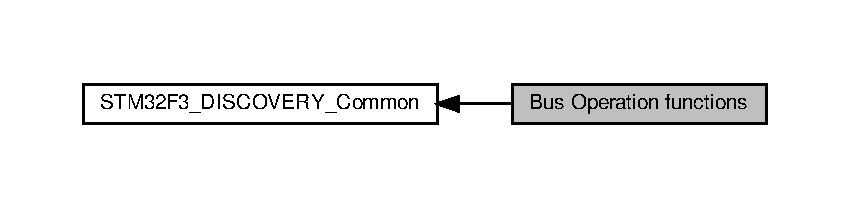
\includegraphics[width=350pt]{group__STM32F3__DISCOVERY__BUS}
\end{center}
\end{figure}


\subsection{Detailed Description}


\subsection{Function Documentation}
\mbox{\Hypertarget{group__STM32F3__DISCOVERY__BUS_ga8361271ff9fae68927a67c607e431eab}\label{group__STM32F3__DISCOVERY__BUS_ga8361271ff9fae68927a67c607e431eab}} 
\index{Bus Operation functions@{Bus Operation functions}!I2\+Cx\+\_\+\+Error@{I2\+Cx\+\_\+\+Error}}
\index{I2\+Cx\+\_\+\+Error@{I2\+Cx\+\_\+\+Error}!Bus Operation functions@{Bus Operation functions}}
\subsubsection{\texorpdfstring{I2\+Cx\+\_\+\+Error()}{I2Cx\_Error()}}
{\footnotesize\ttfamily static void I2\+Cx\+\_\+\+Error (\begin{DoxyParamCaption}\item[{void}]{ }\end{DoxyParamCaption})\hspace{0.3cm}{\ttfamily [static]}}



I2\+C3 error treatment function. 


\begin{DoxyRetVals}{Return values}
{\em None} & \\
\hline
\end{DoxyRetVals}
\mbox{\Hypertarget{group__STM32F3__DISCOVERY__BUS_ga73173918954bb7c4d175c84d0397ae5f}\label{group__STM32F3__DISCOVERY__BUS_ga73173918954bb7c4d175c84d0397ae5f}} 
\index{Bus Operation functions@{Bus Operation functions}!I2\+Cx\+\_\+\+Init@{I2\+Cx\+\_\+\+Init}}
\index{I2\+Cx\+\_\+\+Init@{I2\+Cx\+\_\+\+Init}!Bus Operation functions@{Bus Operation functions}}
\subsubsection{\texorpdfstring{I2\+Cx\+\_\+\+Init()}{I2Cx\_Init()}}
{\footnotesize\ttfamily static void I2\+Cx\+\_\+\+Init (\begin{DoxyParamCaption}\item[{void}]{ }\end{DoxyParamCaption})\hspace{0.3cm}{\ttfamily [static]}}



Discovery I2\+Cx Bus initialization. 


\begin{DoxyRetVals}{Return values}
{\em None} & \\
\hline
\end{DoxyRetVals}
\mbox{\Hypertarget{group__STM32F3__DISCOVERY__BUS_ga659d63031419804f85e3590de210b5c6}\label{group__STM32F3__DISCOVERY__BUS_ga659d63031419804f85e3590de210b5c6}} 
\index{Bus Operation functions@{Bus Operation functions}!I2\+Cx\+\_\+\+Msp\+Init@{I2\+Cx\+\_\+\+Msp\+Init}}
\index{I2\+Cx\+\_\+\+Msp\+Init@{I2\+Cx\+\_\+\+Msp\+Init}!Bus Operation functions@{Bus Operation functions}}
\subsubsection{\texorpdfstring{I2\+Cx\+\_\+\+Msp\+Init()}{I2Cx\_MspInit()}}
{\footnotesize\ttfamily static void I2\+Cx\+\_\+\+Msp\+Init (\begin{DoxyParamCaption}\item[{I2\+C\+\_\+\+Handle\+Type\+Def $\ast$}]{hi2c }\end{DoxyParamCaption})\hspace{0.3cm}{\ttfamily [static]}}



Discovery I2\+Cx M\+SP Initialization. 


\begin{DoxyParams}{Parameters}
{\em hi2c} & I2C handle \\
\hline
\end{DoxyParams}

\begin{DoxyRetVals}{Return values}
{\em None} & \\
\hline
\end{DoxyRetVals}
\mbox{\Hypertarget{group__STM32F3__DISCOVERY__BUS_gafea397a7a4aa6c24435397d6a1e681a8}\label{group__STM32F3__DISCOVERY__BUS_gafea397a7a4aa6c24435397d6a1e681a8}} 
\index{Bus Operation functions@{Bus Operation functions}!I2\+Cx\+\_\+\+Read\+Data@{I2\+Cx\+\_\+\+Read\+Data}}
\index{I2\+Cx\+\_\+\+Read\+Data@{I2\+Cx\+\_\+\+Read\+Data}!Bus Operation functions@{Bus Operation functions}}
\subsubsection{\texorpdfstring{I2\+Cx\+\_\+\+Read\+Data()}{I2Cx\_ReadData()}}
{\footnotesize\ttfamily static uint8\+\_\+t I2\+Cx\+\_\+\+Read\+Data (\begin{DoxyParamCaption}\item[{uint16\+\_\+t}]{Addr,  }\item[{uint8\+\_\+t}]{Reg }\end{DoxyParamCaption})\hspace{0.3cm}{\ttfamily [static]}}



Read a value in a register of the device through B\+US. 


\begin{DoxyParams}{Parameters}
{\em Addr} & Device address on B\+US Bus. \\
\hline
{\em Reg} & The target register address to write \\
\hline
\end{DoxyParams}

\begin{DoxyRetVals}{Return values}
{\em Data} & read at register @ \\
\hline
\end{DoxyRetVals}
\mbox{\Hypertarget{group__STM32F3__DISCOVERY__BUS_ga073ead3d65fe41a407171480f9c0b74e}\label{group__STM32F3__DISCOVERY__BUS_ga073ead3d65fe41a407171480f9c0b74e}} 
\index{Bus Operation functions@{Bus Operation functions}!I2\+Cx\+\_\+\+Write\+Data@{I2\+Cx\+\_\+\+Write\+Data}}
\index{I2\+Cx\+\_\+\+Write\+Data@{I2\+Cx\+\_\+\+Write\+Data}!Bus Operation functions@{Bus Operation functions}}
\subsubsection{\texorpdfstring{I2\+Cx\+\_\+\+Write\+Data()}{I2Cx\_WriteData()}}
{\footnotesize\ttfamily static void I2\+Cx\+\_\+\+Write\+Data (\begin{DoxyParamCaption}\item[{uint16\+\_\+t}]{Addr,  }\item[{uint8\+\_\+t}]{Reg,  }\item[{uint8\+\_\+t}]{Value }\end{DoxyParamCaption})\hspace{0.3cm}{\ttfamily [static]}}



Write a value in a register of the device through B\+US. 


\begin{DoxyParams}{Parameters}
{\em Addr} & Device address on B\+US Bus. \\
\hline
{\em Reg} & The target register address to write \\
\hline
{\em Value} & The target register value to be written \\
\hline
\end{DoxyParams}

\begin{DoxyRetVals}{Return values}
{\em None} & \\
\hline
\end{DoxyRetVals}
\mbox{\Hypertarget{group__STM32F3__DISCOVERY__BUS_ga05479250053954dce6706c7c64fbc746}\label{group__STM32F3__DISCOVERY__BUS_ga05479250053954dce6706c7c64fbc746}} 
\index{Bus Operation functions@{Bus Operation functions}!S\+P\+Ix\+\_\+\+Error@{S\+P\+Ix\+\_\+\+Error}}
\index{S\+P\+Ix\+\_\+\+Error@{S\+P\+Ix\+\_\+\+Error}!Bus Operation functions@{Bus Operation functions}}
\subsubsection{\texorpdfstring{S\+P\+Ix\+\_\+\+Error()}{SPIx\_Error()}}
{\footnotesize\ttfamily static void S\+P\+Ix\+\_\+\+Error (\begin{DoxyParamCaption}\item[{void}]{ }\end{DoxyParamCaption})\hspace{0.3cm}{\ttfamily [static]}}



S\+P\+Ix error treatment function. 


\begin{DoxyRetVals}{Return values}
{\em None} & \\
\hline
\end{DoxyRetVals}
\mbox{\Hypertarget{group__STM32F3__DISCOVERY__BUS_ga411b8bc3e3c513999639449b40dca4a2}\label{group__STM32F3__DISCOVERY__BUS_ga411b8bc3e3c513999639449b40dca4a2}} 
\index{Bus Operation functions@{Bus Operation functions}!S\+P\+Ix\+\_\+\+Init@{S\+P\+Ix\+\_\+\+Init}}
\index{S\+P\+Ix\+\_\+\+Init@{S\+P\+Ix\+\_\+\+Init}!Bus Operation functions@{Bus Operation functions}}
\subsubsection{\texorpdfstring{S\+P\+Ix\+\_\+\+Init()}{SPIx\_Init()}}
{\footnotesize\ttfamily static void S\+P\+Ix\+\_\+\+Init (\begin{DoxyParamCaption}\item[{void}]{ }\end{DoxyParamCaption})\hspace{0.3cm}{\ttfamily [static]}}



S\+P\+Ix Bus initialization. 


\begin{DoxyRetVals}{Return values}
{\em None} & \\
\hline
\end{DoxyRetVals}
\mbox{\Hypertarget{group__STM32F3__DISCOVERY__BUS_gac2a32a81a80a73a794887876add1b82d}\label{group__STM32F3__DISCOVERY__BUS_gac2a32a81a80a73a794887876add1b82d}} 
\index{Bus Operation functions@{Bus Operation functions}!S\+P\+Ix\+\_\+\+Msp\+Init@{S\+P\+Ix\+\_\+\+Msp\+Init}}
\index{S\+P\+Ix\+\_\+\+Msp\+Init@{S\+P\+Ix\+\_\+\+Msp\+Init}!Bus Operation functions@{Bus Operation functions}}
\subsubsection{\texorpdfstring{S\+P\+Ix\+\_\+\+Msp\+Init()}{SPIx\_MspInit()}}
{\footnotesize\ttfamily static void S\+P\+Ix\+\_\+\+Msp\+Init (\begin{DoxyParamCaption}\item[{S\+P\+I\+\_\+\+Handle\+Type\+Def $\ast$}]{hspi }\end{DoxyParamCaption})\hspace{0.3cm}{\ttfamily [static]}}



S\+PI M\+SP Init. 


\begin{DoxyParams}{Parameters}
{\em hspi} & S\+PI handle \\
\hline
\end{DoxyParams}

\begin{DoxyRetVals}{Return values}
{\em None} & \\
\hline
\end{DoxyRetVals}
\mbox{\Hypertarget{group__STM32F3__DISCOVERY__BUS_gaca16be8c665e3e886f1b7333dd778728}\label{group__STM32F3__DISCOVERY__BUS_gaca16be8c665e3e886f1b7333dd778728}} 
\index{Bus Operation functions@{Bus Operation functions}!S\+P\+Ix\+\_\+\+Write\+Read@{S\+P\+Ix\+\_\+\+Write\+Read}}
\index{S\+P\+Ix\+\_\+\+Write\+Read@{S\+P\+Ix\+\_\+\+Write\+Read}!Bus Operation functions@{Bus Operation functions}}
\subsubsection{\texorpdfstring{S\+P\+Ix\+\_\+\+Write\+Read()}{SPIx\_WriteRead()}}
{\footnotesize\ttfamily static uint8\+\_\+t S\+P\+Ix\+\_\+\+Write\+Read (\begin{DoxyParamCaption}\item[{uint8\+\_\+t}]{Byte }\end{DoxyParamCaption})\hspace{0.3cm}{\ttfamily [static]}}



Sends a Byte through the S\+PI interface and return the Byte received from the S\+PI bus. 


\begin{DoxyParams}{Parameters}
{\em Byte} & Byte send. \\
\hline
\end{DoxyParams}

\begin{DoxyRetVals}{Return values}
{\em The} & received byte value \\
\hline
\end{DoxyRetVals}

\hypertarget{group__STM32F3__DISCOVERY__LINK__OPERATIONS}{}\section{Link Operation functions}
\label{group__STM32F3__DISCOVERY__LINK__OPERATIONS}\index{Link Operation functions@{Link Operation functions}}
Collaboration diagram for Link Operation functions\+:\nopagebreak
\begin{figure}[H]
\begin{center}
\leavevmode
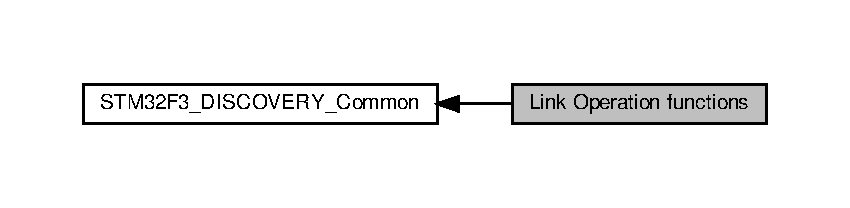
\includegraphics[width=350pt]{group__STM32F3__DISCOVERY__LINK__OPERATIONS}
\end{center}
\end{figure}


\subsection{Detailed Description}


\subsection{Function Documentation}
\mbox{\Hypertarget{group__STM32F3__DISCOVERY__LINK__OPERATIONS_ga7ce9cc034e3d64924bd88adae6770d19}\label{group__STM32F3__DISCOVERY__LINK__OPERATIONS_ga7ce9cc034e3d64924bd88adae6770d19}} 
\index{Link Operation functions@{Link Operation functions}!C\+O\+M\+P\+A\+S\+S\+A\+C\+C\+E\+L\+E\+R\+O\+\_\+\+I\+O\+\_\+\+Init@{C\+O\+M\+P\+A\+S\+S\+A\+C\+C\+E\+L\+E\+R\+O\+\_\+\+I\+O\+\_\+\+Init}}
\index{C\+O\+M\+P\+A\+S\+S\+A\+C\+C\+E\+L\+E\+R\+O\+\_\+\+I\+O\+\_\+\+Init@{C\+O\+M\+P\+A\+S\+S\+A\+C\+C\+E\+L\+E\+R\+O\+\_\+\+I\+O\+\_\+\+Init}!Link Operation functions@{Link Operation functions}}
\subsubsection{\texorpdfstring{C\+O\+M\+P\+A\+S\+S\+A\+C\+C\+E\+L\+E\+R\+O\+\_\+\+I\+O\+\_\+\+Init()}{COMPASSACCELERO\_IO\_Init()}}
{\footnotesize\ttfamily void C\+O\+M\+P\+A\+S\+S\+A\+C\+C\+E\+L\+E\+R\+O\+\_\+\+I\+O\+\_\+\+Init (\begin{DoxyParamCaption}\item[{void}]{ }\end{DoxyParamCaption})}



Configures C\+O\+M\+P\+A\+SS / A\+C\+C\+E\+L\+E\+R\+O\+M\+E\+T\+ER I2C interface. 


\begin{DoxyRetVals}{Return values}
{\em None} & \\
\hline
\end{DoxyRetVals}
\mbox{\Hypertarget{group__STM32F3__DISCOVERY__LINK__OPERATIONS_ga0d94d79fddfe98ed16c8c63c65f186db}\label{group__STM32F3__DISCOVERY__LINK__OPERATIONS_ga0d94d79fddfe98ed16c8c63c65f186db}} 
\index{Link Operation functions@{Link Operation functions}!C\+O\+M\+P\+A\+S\+S\+A\+C\+C\+E\+L\+E\+R\+O\+\_\+\+I\+O\+\_\+\+I\+T\+Config@{C\+O\+M\+P\+A\+S\+S\+A\+C\+C\+E\+L\+E\+R\+O\+\_\+\+I\+O\+\_\+\+I\+T\+Config}}
\index{C\+O\+M\+P\+A\+S\+S\+A\+C\+C\+E\+L\+E\+R\+O\+\_\+\+I\+O\+\_\+\+I\+T\+Config@{C\+O\+M\+P\+A\+S\+S\+A\+C\+C\+E\+L\+E\+R\+O\+\_\+\+I\+O\+\_\+\+I\+T\+Config}!Link Operation functions@{Link Operation functions}}
\subsubsection{\texorpdfstring{C\+O\+M\+P\+A\+S\+S\+A\+C\+C\+E\+L\+E\+R\+O\+\_\+\+I\+O\+\_\+\+I\+T\+Config()}{COMPASSACCELERO\_IO\_ITConfig()}}
{\footnotesize\ttfamily void C\+O\+M\+P\+A\+S\+S\+A\+C\+C\+E\+L\+E\+R\+O\+\_\+\+I\+O\+\_\+\+I\+T\+Config (\begin{DoxyParamCaption}\item[{void}]{ }\end{DoxyParamCaption})}



Configures C\+O\+M\+P\+A\+SS / A\+C\+C\+E\+L\+E\+RO click IT. 


\begin{DoxyRetVals}{Return values}
{\em None} & \\
\hline
\end{DoxyRetVals}
\mbox{\Hypertarget{group__STM32F3__DISCOVERY__LINK__OPERATIONS_ga2d4c2b7ccef8b3be4cf0335e9fcffd2f}\label{group__STM32F3__DISCOVERY__LINK__OPERATIONS_ga2d4c2b7ccef8b3be4cf0335e9fcffd2f}} 
\index{Link Operation functions@{Link Operation functions}!C\+O\+M\+P\+A\+S\+S\+A\+C\+C\+E\+L\+E\+R\+O\+\_\+\+I\+O\+\_\+\+Read@{C\+O\+M\+P\+A\+S\+S\+A\+C\+C\+E\+L\+E\+R\+O\+\_\+\+I\+O\+\_\+\+Read}}
\index{C\+O\+M\+P\+A\+S\+S\+A\+C\+C\+E\+L\+E\+R\+O\+\_\+\+I\+O\+\_\+\+Read@{C\+O\+M\+P\+A\+S\+S\+A\+C\+C\+E\+L\+E\+R\+O\+\_\+\+I\+O\+\_\+\+Read}!Link Operation functions@{Link Operation functions}}
\subsubsection{\texorpdfstring{C\+O\+M\+P\+A\+S\+S\+A\+C\+C\+E\+L\+E\+R\+O\+\_\+\+I\+O\+\_\+\+Read()}{COMPASSACCELERO\_IO\_Read()}}
{\footnotesize\ttfamily uint8\+\_\+t C\+O\+M\+P\+A\+S\+S\+A\+C\+C\+E\+L\+E\+R\+O\+\_\+\+I\+O\+\_\+\+Read (\begin{DoxyParamCaption}\item[{uint16\+\_\+t}]{Device\+Addr,  }\item[{uint8\+\_\+t}]{Register\+Addr }\end{DoxyParamCaption})}



Reads a block of data from the C\+O\+M\+P\+A\+SS / A\+C\+C\+E\+L\+E\+R\+O\+M\+E\+T\+ER. 


\begin{DoxyParams}{Parameters}
{\em Device\+Addr} & specifies the slave address to be programmed(\+A\+C\+C\+\_\+\+I2\+C\+\_\+\+A\+D\+D\+R\+E\+S\+S or M\+A\+G\+\_\+\+I2\+C\+\_\+\+A\+D\+D\+R\+E\+S\+S). \\
\hline
{\em Register\+Addr} & specifies the C\+O\+M\+P\+A\+SS / A\+C\+C\+E\+L\+E\+R\+O\+M\+E\+T\+ER internal address register to read from \\
\hline
\end{DoxyParams}

\begin{DoxyRetVals}{Return values}
{\em A\+C\+C\+E\+L\+E\+R\+O\+M\+E\+T\+ER} & register value \\
\hline
\end{DoxyRetVals}
\mbox{\Hypertarget{group__STM32F3__DISCOVERY__LINK__OPERATIONS_gad84492b8ff84b8112e4e93d35d67f116}\label{group__STM32F3__DISCOVERY__LINK__OPERATIONS_gad84492b8ff84b8112e4e93d35d67f116}} 
\index{Link Operation functions@{Link Operation functions}!C\+O\+M\+P\+A\+S\+S\+A\+C\+C\+E\+L\+E\+R\+O\+\_\+\+I\+O\+\_\+\+Write@{C\+O\+M\+P\+A\+S\+S\+A\+C\+C\+E\+L\+E\+R\+O\+\_\+\+I\+O\+\_\+\+Write}}
\index{C\+O\+M\+P\+A\+S\+S\+A\+C\+C\+E\+L\+E\+R\+O\+\_\+\+I\+O\+\_\+\+Write@{C\+O\+M\+P\+A\+S\+S\+A\+C\+C\+E\+L\+E\+R\+O\+\_\+\+I\+O\+\_\+\+Write}!Link Operation functions@{Link Operation functions}}
\subsubsection{\texorpdfstring{C\+O\+M\+P\+A\+S\+S\+A\+C\+C\+E\+L\+E\+R\+O\+\_\+\+I\+O\+\_\+\+Write()}{COMPASSACCELERO\_IO\_Write()}}
{\footnotesize\ttfamily void C\+O\+M\+P\+A\+S\+S\+A\+C\+C\+E\+L\+E\+R\+O\+\_\+\+I\+O\+\_\+\+Write (\begin{DoxyParamCaption}\item[{uint16\+\_\+t}]{Device\+Addr,  }\item[{uint8\+\_\+t}]{Register\+Addr,  }\item[{uint8\+\_\+t}]{Value }\end{DoxyParamCaption})}



Writes one byte to the C\+O\+M\+P\+A\+SS / A\+C\+C\+E\+L\+E\+R\+O\+M\+E\+T\+ER. 


\begin{DoxyParams}{Parameters}
{\em Device\+Addr} & specifies the slave address to be programmed. \\
\hline
{\em Register\+Addr} & specifies the C\+O\+M\+P\+A\+SS / A\+C\+C\+E\+L\+E\+R\+O\+M\+E\+T\+ER register to be written. \\
\hline
{\em Value} & Data to be written \\
\hline
\end{DoxyParams}

\begin{DoxyRetVals}{Return values}
{\em None} & \\
\hline
\end{DoxyRetVals}
\mbox{\Hypertarget{group__STM32F3__DISCOVERY__LINK__OPERATIONS_gab11396b3a6f76ba95ea19290c7e60da5}\label{group__STM32F3__DISCOVERY__LINK__OPERATIONS_gab11396b3a6f76ba95ea19290c7e60da5}} 
\index{Link Operation functions@{Link Operation functions}!G\+Y\+R\+O\+\_\+\+I\+O\+\_\+\+Init@{G\+Y\+R\+O\+\_\+\+I\+O\+\_\+\+Init}}
\index{G\+Y\+R\+O\+\_\+\+I\+O\+\_\+\+Init@{G\+Y\+R\+O\+\_\+\+I\+O\+\_\+\+Init}!Link Operation functions@{Link Operation functions}}
\subsubsection{\texorpdfstring{G\+Y\+R\+O\+\_\+\+I\+O\+\_\+\+Init()}{GYRO\_IO\_Init()}}
{\footnotesize\ttfamily void G\+Y\+R\+O\+\_\+\+I\+O\+\_\+\+Init (\begin{DoxyParamCaption}\item[{void}]{ }\end{DoxyParamCaption})}



Configures the G\+Y\+R\+O\+S\+C\+O\+PE S\+PI interface. 


\begin{DoxyRetVals}{Return values}
{\em None} & \\
\hline
\end{DoxyRetVals}
\mbox{\Hypertarget{group__STM32F3__DISCOVERY__LINK__OPERATIONS_ga1432dd354981626497d038b4f7149b92}\label{group__STM32F3__DISCOVERY__LINK__OPERATIONS_ga1432dd354981626497d038b4f7149b92}} 
\index{Link Operation functions@{Link Operation functions}!G\+Y\+R\+O\+\_\+\+I\+O\+\_\+\+Read@{G\+Y\+R\+O\+\_\+\+I\+O\+\_\+\+Read}}
\index{G\+Y\+R\+O\+\_\+\+I\+O\+\_\+\+Read@{G\+Y\+R\+O\+\_\+\+I\+O\+\_\+\+Read}!Link Operation functions@{Link Operation functions}}
\subsubsection{\texorpdfstring{G\+Y\+R\+O\+\_\+\+I\+O\+\_\+\+Read()}{GYRO\_IO\_Read()}}
{\footnotesize\ttfamily void G\+Y\+R\+O\+\_\+\+I\+O\+\_\+\+Read (\begin{DoxyParamCaption}\item[{uint8\+\_\+t$\ast$}]{p\+Buffer,  }\item[{uint8\+\_\+t}]{Read\+Addr,  }\item[{uint16\+\_\+t}]{Num\+Byte\+To\+Read }\end{DoxyParamCaption})}



Reads a block of data from the G\+Y\+R\+O\+S\+C\+O\+PE. 


\begin{DoxyParams}{Parameters}
{\em p\+Buffer} & pointer to the buffer that receives the data read from the G\+Y\+R\+O\+S\+C\+O\+PE. \\
\hline
{\em Read\+Addr} & G\+Y\+R\+O\+S\+C\+O\+PE\textquotesingle{}s internal address to read from. \\
\hline
{\em Num\+Byte\+To\+Read} & number of bytes to read from the G\+Y\+R\+O\+S\+C\+O\+PE. \\
\hline
\end{DoxyParams}

\begin{DoxyRetVals}{Return values}
{\em None} & \\
\hline
\end{DoxyRetVals}
\mbox{\Hypertarget{group__STM32F3__DISCOVERY__LINK__OPERATIONS_ga5d9e3e80db2ee7cb6d8bd2f92d25b339}\label{group__STM32F3__DISCOVERY__LINK__OPERATIONS_ga5d9e3e80db2ee7cb6d8bd2f92d25b339}} 
\index{Link Operation functions@{Link Operation functions}!G\+Y\+R\+O\+\_\+\+I\+O\+\_\+\+Write@{G\+Y\+R\+O\+\_\+\+I\+O\+\_\+\+Write}}
\index{G\+Y\+R\+O\+\_\+\+I\+O\+\_\+\+Write@{G\+Y\+R\+O\+\_\+\+I\+O\+\_\+\+Write}!Link Operation functions@{Link Operation functions}}
\subsubsection{\texorpdfstring{G\+Y\+R\+O\+\_\+\+I\+O\+\_\+\+Write()}{GYRO\_IO\_Write()}}
{\footnotesize\ttfamily void G\+Y\+R\+O\+\_\+\+I\+O\+\_\+\+Write (\begin{DoxyParamCaption}\item[{uint8\+\_\+t$\ast$}]{p\+Buffer,  }\item[{uint8\+\_\+t}]{Write\+Addr,  }\item[{uint16\+\_\+t}]{Num\+Byte\+To\+Write }\end{DoxyParamCaption})}



Writes one byte to the G\+Y\+R\+O\+S\+C\+O\+PE. 


\begin{DoxyParams}{Parameters}
{\em p\+Buffer} & pointer to the buffer containing the data to be written to the G\+Y\+R\+O\+S\+C\+O\+PE. \\
\hline
{\em Write\+Addr} & G\+Y\+R\+O\+S\+C\+O\+PE\textquotesingle{}s internal address to write to. \\
\hline
{\em Num\+Byte\+To\+Write} & Number of bytes to write. \\
\hline
\end{DoxyParams}

\begin{DoxyRetVals}{Return values}
{\em None} & \\
\hline
\end{DoxyRetVals}

\hypertarget{group__STM32F3__DISCOVERY__Exported__Constants}{}\section{Exported Constants}
\label{group__STM32F3__DISCOVERY__Exported__Constants}\index{Exported Constants@{Exported Constants}}
Collaboration diagram for Exported Constants\+:\nopagebreak
\begin{figure}[H]
\begin{center}
\leavevmode
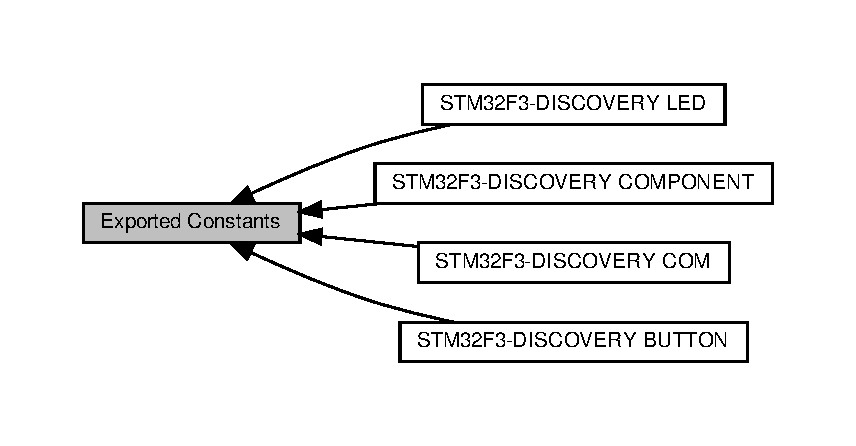
\includegraphics[width=350pt]{group__STM32F3__DISCOVERY__Exported__Constants}
\end{center}
\end{figure}
\subsection*{Modules}
\begin{DoxyCompactItemize}
\item 
\hyperlink{group__STM32F3__DISCOVERY__LED}{S\+T\+M32\+F3-\/\+D\+I\+S\+C\+O\+V\+E\+R\+Y L\+ED}
\item 
\hyperlink{group__STM32F3__DISCOVERY__BUTTON}{S\+T\+M32\+F3-\/\+D\+I\+S\+C\+O\+V\+E\+R\+Y B\+U\+T\+T\+ON}
\item 
\hyperlink{group__STM32F3__DISCOVERY__COM}{S\+T\+M32\+F3-\/\+D\+I\+S\+C\+O\+V\+E\+R\+Y C\+OM}
\item 
\hyperlink{group__STM32F3__DISCOVERY__COMPONENT}{S\+T\+M32\+F3-\/\+D\+I\+S\+C\+O\+V\+E\+R\+Y C\+O\+M\+P\+O\+N\+E\+NT}
\end{DoxyCompactItemize}


\subsection{Detailed Description}

\hypertarget{group__STM32F3__DISCOVERY__LED}{}\section{S\+T\+M32\+F3-\/\+D\+I\+S\+C\+O\+V\+E\+RY L\+ED}
\label{group__STM32F3__DISCOVERY__LED}\index{S\+T\+M32\+F3-\/\+D\+I\+S\+C\+O\+V\+E\+R\+Y L\+ED@{S\+T\+M32\+F3-\/\+D\+I\+S\+C\+O\+V\+E\+R\+Y L\+ED}}
Collaboration diagram for S\+T\+M32\+F3-\/\+D\+I\+S\+C\+O\+V\+E\+RY L\+ED\+:\nopagebreak
\begin{figure}[H]
\begin{center}
\leavevmode
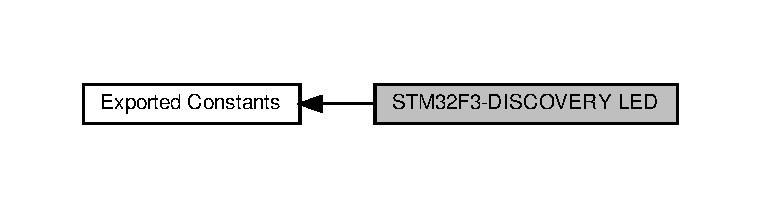
\includegraphics[width=350pt]{group__STM32F3__DISCOVERY__LED}
\end{center}
\end{figure}

\hypertarget{group__STM32F3__DISCOVERY__BUTTON}{}\section{S\+T\+M32\+F3-\/\+D\+I\+S\+C\+O\+V\+E\+RY B\+U\+T\+T\+ON}
\label{group__STM32F3__DISCOVERY__BUTTON}\index{S\+T\+M32\+F3-\/\+D\+I\+S\+C\+O\+V\+E\+R\+Y B\+U\+T\+T\+ON@{S\+T\+M32\+F3-\/\+D\+I\+S\+C\+O\+V\+E\+R\+Y B\+U\+T\+T\+ON}}
Collaboration diagram for S\+T\+M32\+F3-\/\+D\+I\+S\+C\+O\+V\+E\+RY B\+U\+T\+T\+ON\+:\nopagebreak
\begin{figure}[H]
\begin{center}
\leavevmode
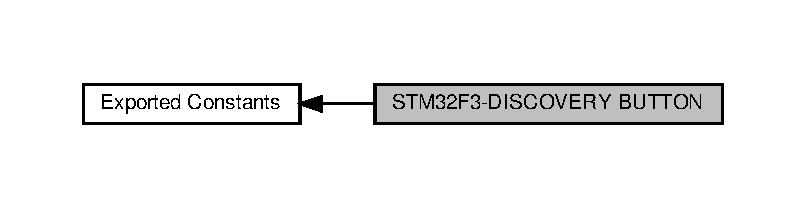
\includegraphics[width=350pt]{group__STM32F3__DISCOVERY__BUTTON}
\end{center}
\end{figure}

\hypertarget{group__STM32F3__DISCOVERY__COM}{}\section{S\+T\+M32\+F3-\/\+D\+I\+S\+C\+O\+V\+E\+RY C\+OM}
\label{group__STM32F3__DISCOVERY__COM}\index{S\+T\+M32\+F3-\/\+D\+I\+S\+C\+O\+V\+E\+R\+Y C\+OM@{S\+T\+M32\+F3-\/\+D\+I\+S\+C\+O\+V\+E\+R\+Y C\+OM}}
Collaboration diagram for S\+T\+M32\+F3-\/\+D\+I\+S\+C\+O\+V\+E\+RY C\+OM\+:\nopagebreak
\begin{figure}[H]
\begin{center}
\leavevmode
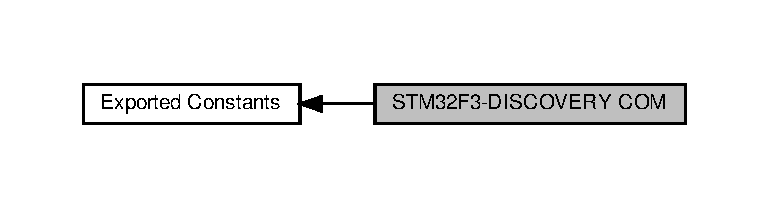
\includegraphics[width=350pt]{group__STM32F3__DISCOVERY__COM}
\end{center}
\end{figure}

\hypertarget{group__STM32F3__DISCOVERY__COMPONENT}{}\section{S\+T\+M32\+F3-\/\+D\+I\+S\+C\+O\+V\+E\+RY C\+O\+M\+P\+O\+N\+E\+NT}
\label{group__STM32F3__DISCOVERY__COMPONENT}\index{S\+T\+M32\+F3-\/\+D\+I\+S\+C\+O\+V\+E\+R\+Y C\+O\+M\+P\+O\+N\+E\+NT@{S\+T\+M32\+F3-\/\+D\+I\+S\+C\+O\+V\+E\+R\+Y C\+O\+M\+P\+O\+N\+E\+NT}}
Collaboration diagram for S\+T\+M32\+F3-\/\+D\+I\+S\+C\+O\+V\+E\+RY C\+O\+M\+P\+O\+N\+E\+NT\+:\nopagebreak
\begin{figure}[H]
\begin{center}
\leavevmode
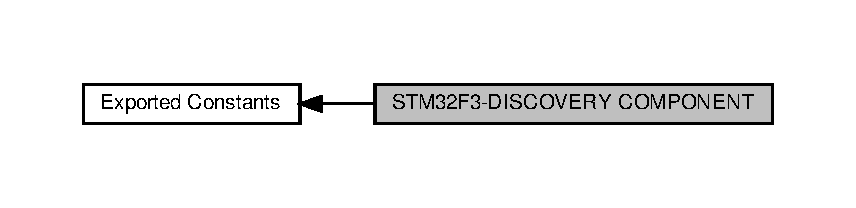
\includegraphics[width=350pt]{group__STM32F3__DISCOVERY__COMPONENT}
\end{center}
\end{figure}

\hypertarget{group__STM32F3__DISCOVERY__Exported__Functions}{}\section{Exported Functions}
\label{group__STM32F3__DISCOVERY__Exported__Functions}\index{Exported Functions@{Exported Functions}}
Collaboration diagram for Exported Functions\+:\nopagebreak
\begin{figure}[H]
\begin{center}
\leavevmode
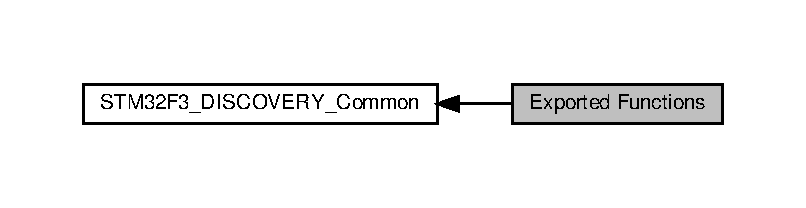
\includegraphics[width=350pt]{group__STM32F3__DISCOVERY__Exported__Functions}
\end{center}
\end{figure}


\subsection{Detailed Description}


\subsection{Function Documentation}
\mbox{\Hypertarget{group__STM32F3__DISCOVERY__Exported__Functions_ga88eb8fe79668f12714ed74ed9ad661ff}\label{group__STM32F3__DISCOVERY__Exported__Functions_ga88eb8fe79668f12714ed74ed9ad661ff}} 
\index{Exported Functions@{Exported Functions}!B\+S\+P\+\_\+\+Get\+Version@{B\+S\+P\+\_\+\+Get\+Version}}
\index{B\+S\+P\+\_\+\+Get\+Version@{B\+S\+P\+\_\+\+Get\+Version}!Exported Functions@{Exported Functions}}
\subsubsection{\texorpdfstring{B\+S\+P\+\_\+\+Get\+Version()}{BSP\_GetVersion()}}
{\footnotesize\ttfamily uint32\+\_\+t B\+S\+P\+\_\+\+Get\+Version (\begin{DoxyParamCaption}\item[{void}]{ }\end{DoxyParamCaption})}



This method returns the S\+T\+M32\+F3-\/\+D\+I\+S\+C\+O\+V\+E\+RY B\+SP Driver revision. 


\begin{DoxyRetVals}{Return values}
{\em version} & \+: 0x\+X\+Y\+ZR (8bits for each decimal, R for RC) \\
\hline
\end{DoxyRetVals}
\mbox{\Hypertarget{group__STM32F3__DISCOVERY__Exported__Functions_gac1524552e5089ce37457e6df6bac86b6}\label{group__STM32F3__DISCOVERY__Exported__Functions_gac1524552e5089ce37457e6df6bac86b6}} 
\index{Exported Functions@{Exported Functions}!B\+S\+P\+\_\+\+L\+E\+D\+\_\+\+Init@{B\+S\+P\+\_\+\+L\+E\+D\+\_\+\+Init}}
\index{B\+S\+P\+\_\+\+L\+E\+D\+\_\+\+Init@{B\+S\+P\+\_\+\+L\+E\+D\+\_\+\+Init}!Exported Functions@{Exported Functions}}
\subsubsection{\texorpdfstring{B\+S\+P\+\_\+\+L\+E\+D\+\_\+\+Init()}{BSP\_LED\_Init()}}
{\footnotesize\ttfamily void B\+S\+P\+\_\+\+L\+E\+D\+\_\+\+Init (\begin{DoxyParamCaption}\item[{Led\+\_\+\+Type\+Def}]{Led }\end{DoxyParamCaption})}



Configures L\+ED \hyperlink{structGPIO}{G\+P\+IO}. 


\begin{DoxyParams}{Parameters}
{\em Led} & Specifies the Led to be configured. This parameter can be one of following parameters\+: \begin{DoxyItemize}
\item L\+E\+D\+\_\+\+R\+ED \item L\+E\+D\+\_\+\+B\+L\+UE \item L\+E\+D\+\_\+\+O\+R\+A\+N\+GE \item L\+E\+D\+\_\+\+G\+R\+E\+EN \item L\+E\+D\+\_\+\+G\+R\+E\+E\+N2 \item L\+E\+D\+\_\+\+O\+R\+A\+N\+G\+E2 \item L\+E\+D\+\_\+\+B\+L\+U\+E2 \item L\+E\+D\+\_\+\+R\+E\+D2 \end{DoxyItemize}
\\
\hline
\end{DoxyParams}

\begin{DoxyRetVals}{Return values}
{\em None} & \\
\hline
\end{DoxyRetVals}
\mbox{\Hypertarget{group__STM32F3__DISCOVERY__Exported__Functions_ga939ab765378718b3c299734391cbd4dd}\label{group__STM32F3__DISCOVERY__Exported__Functions_ga939ab765378718b3c299734391cbd4dd}} 
\index{Exported Functions@{Exported Functions}!B\+S\+P\+\_\+\+L\+E\+D\+\_\+\+Off@{B\+S\+P\+\_\+\+L\+E\+D\+\_\+\+Off}}
\index{B\+S\+P\+\_\+\+L\+E\+D\+\_\+\+Off@{B\+S\+P\+\_\+\+L\+E\+D\+\_\+\+Off}!Exported Functions@{Exported Functions}}
\subsubsection{\texorpdfstring{B\+S\+P\+\_\+\+L\+E\+D\+\_\+\+Off()}{BSP\_LED\_Off()}}
{\footnotesize\ttfamily void B\+S\+P\+\_\+\+L\+E\+D\+\_\+\+Off (\begin{DoxyParamCaption}\item[{Led\+\_\+\+Type\+Def}]{Led }\end{DoxyParamCaption})}



Turns selected L\+ED Off. 


\begin{DoxyParams}{Parameters}
{\em Led} & Specifies the Led to be set off. This parameter can be one of following parameters\+: \begin{DoxyItemize}
\item L\+E\+D\+\_\+\+R\+ED \item L\+E\+D\+\_\+\+B\+L\+UE \item L\+E\+D\+\_\+\+O\+R\+A\+N\+GE \item L\+E\+D\+\_\+\+G\+R\+E\+EN \item L\+E\+D\+\_\+\+G\+R\+E\+E\+N2 \item L\+E\+D\+\_\+\+O\+R\+A\+N\+G\+E2 \item L\+E\+D\+\_\+\+B\+L\+U\+E2 \item L\+E\+D\+\_\+\+R\+E\+D2 \end{DoxyItemize}
\\
\hline
\end{DoxyParams}

\begin{DoxyRetVals}{Return values}
{\em None} & \\
\hline
\end{DoxyRetVals}
\mbox{\Hypertarget{group__STM32F3__DISCOVERY__Exported__Functions_gae18974cf5af73c404ae48b90118826cd}\label{group__STM32F3__DISCOVERY__Exported__Functions_gae18974cf5af73c404ae48b90118826cd}} 
\index{Exported Functions@{Exported Functions}!B\+S\+P\+\_\+\+L\+E\+D\+\_\+\+On@{B\+S\+P\+\_\+\+L\+E\+D\+\_\+\+On}}
\index{B\+S\+P\+\_\+\+L\+E\+D\+\_\+\+On@{B\+S\+P\+\_\+\+L\+E\+D\+\_\+\+On}!Exported Functions@{Exported Functions}}
\subsubsection{\texorpdfstring{B\+S\+P\+\_\+\+L\+E\+D\+\_\+\+On()}{BSP\_LED\_On()}}
{\footnotesize\ttfamily void B\+S\+P\+\_\+\+L\+E\+D\+\_\+\+On (\begin{DoxyParamCaption}\item[{Led\+\_\+\+Type\+Def}]{Led }\end{DoxyParamCaption})}



Turns selected L\+ED On. 


\begin{DoxyParams}{Parameters}
{\em Led} & Specifies the Led to be set on. This parameter can be one of following parameters\+: \begin{DoxyItemize}
\item L\+E\+D\+\_\+\+R\+ED \item L\+E\+D4 \item L\+E\+D5 \item L\+E\+D6 \item L\+E\+D7 \item L\+E\+D8 \item L\+E\+D9 \item L\+E\+D10 \end{DoxyItemize}
\\
\hline
\end{DoxyParams}

\begin{DoxyRetVals}{Return values}
{\em None} & \\
\hline
\end{DoxyRetVals}
\mbox{\Hypertarget{group__STM32F3__DISCOVERY__Exported__Functions_ga9fc84071d022ec6c51cdc00969a744e0}\label{group__STM32F3__DISCOVERY__Exported__Functions_ga9fc84071d022ec6c51cdc00969a744e0}} 
\index{Exported Functions@{Exported Functions}!B\+S\+P\+\_\+\+L\+E\+D\+\_\+\+Toggle@{B\+S\+P\+\_\+\+L\+E\+D\+\_\+\+Toggle}}
\index{B\+S\+P\+\_\+\+L\+E\+D\+\_\+\+Toggle@{B\+S\+P\+\_\+\+L\+E\+D\+\_\+\+Toggle}!Exported Functions@{Exported Functions}}
\subsubsection{\texorpdfstring{B\+S\+P\+\_\+\+L\+E\+D\+\_\+\+Toggle()}{BSP\_LED\_Toggle()}}
{\footnotesize\ttfamily void B\+S\+P\+\_\+\+L\+E\+D\+\_\+\+Toggle (\begin{DoxyParamCaption}\item[{Led\+\_\+\+Type\+Def}]{Led }\end{DoxyParamCaption})}



Toggles the selected L\+ED. 


\begin{DoxyParams}{Parameters}
{\em Led} & Specifies the Led to be toggled. This parameter can be one of following parameters\+: \begin{DoxyItemize}
\item L\+E\+D\+\_\+\+R\+ED \item L\+E\+D\+\_\+\+B\+L\+UE \item L\+E\+D\+\_\+\+O\+R\+A\+N\+GE \item L\+E\+D\+\_\+\+G\+R\+E\+EN \item L\+E\+D\+\_\+\+G\+R\+E\+E\+N2 \item L\+E\+D\+\_\+\+O\+R\+A\+N\+G\+E2 \item L\+E\+D\+\_\+\+B\+L\+U\+E2 \item L\+E\+D\+\_\+\+R\+E\+D2 \end{DoxyItemize}
\\
\hline
\end{DoxyParams}

\begin{DoxyRetVals}{Return values}
{\em None} & \\
\hline
\end{DoxyRetVals}
\mbox{\Hypertarget{group__STM32F3__DISCOVERY__Exported__Functions_gac72e738a85fbbbcf26d038dd5c1a9adc}\label{group__STM32F3__DISCOVERY__Exported__Functions_gac72e738a85fbbbcf26d038dd5c1a9adc}} 
\index{Exported Functions@{Exported Functions}!B\+S\+P\+\_\+\+P\+B\+\_\+\+Get\+State@{B\+S\+P\+\_\+\+P\+B\+\_\+\+Get\+State}}
\index{B\+S\+P\+\_\+\+P\+B\+\_\+\+Get\+State@{B\+S\+P\+\_\+\+P\+B\+\_\+\+Get\+State}!Exported Functions@{Exported Functions}}
\subsubsection{\texorpdfstring{B\+S\+P\+\_\+\+P\+B\+\_\+\+Get\+State()}{BSP\_PB\_GetState()}}
{\footnotesize\ttfamily uint32\+\_\+t B\+S\+P\+\_\+\+P\+B\+\_\+\+Get\+State (\begin{DoxyParamCaption}\item[{\hyperlink{stm32f3__discovery_8h_a643816dfbad5c734fc25a29ce8d35bb1}{Button\+\_\+\+Type\+Def}}]{Button }\end{DoxyParamCaption})}



Returns the selected Push Button state. 


\begin{DoxyParams}{Parameters}
{\em Button} & Specifies the Button to be checked. This parameter should be\+: B\+U\+T\+T\+O\+N\+\_\+\+U\+S\+ER \\
\hline
\end{DoxyParams}

\begin{DoxyRetVals}{Return values}
{\em The} & Button \hyperlink{structGPIO}{G\+P\+IO} pin value. \\
\hline
\end{DoxyRetVals}
\mbox{\Hypertarget{group__STM32F3__DISCOVERY__Exported__Functions_ga540042303b6e13d34b8ef06eb771d1b3}\label{group__STM32F3__DISCOVERY__Exported__Functions_ga540042303b6e13d34b8ef06eb771d1b3}} 
\index{Exported Functions@{Exported Functions}!B\+S\+P\+\_\+\+P\+B\+\_\+\+Init@{B\+S\+P\+\_\+\+P\+B\+\_\+\+Init}}
\index{B\+S\+P\+\_\+\+P\+B\+\_\+\+Init@{B\+S\+P\+\_\+\+P\+B\+\_\+\+Init}!Exported Functions@{Exported Functions}}
\subsubsection{\texorpdfstring{B\+S\+P\+\_\+\+P\+B\+\_\+\+Init()}{BSP\_PB\_Init()}}
{\footnotesize\ttfamily void B\+S\+P\+\_\+\+P\+B\+\_\+\+Init (\begin{DoxyParamCaption}\item[{\hyperlink{stm32f3__discovery_8h_a643816dfbad5c734fc25a29ce8d35bb1}{Button\+\_\+\+Type\+Def}}]{Button,  }\item[{Button\+Mode\+\_\+\+Type\+Def}]{Button\+Mode }\end{DoxyParamCaption})}



Configures Push Button \hyperlink{structGPIO}{G\+P\+IO} and E\+X\+TI Line. 


\begin{DoxyParams}{Parameters}
{\em Button} & Specifies the Button to be configured. This parameter should be\+: B\+U\+T\+T\+O\+N\+\_\+\+U\+S\+ER \\
\hline
{\em Button\+Mode} & Specifies Button mode. This parameter can be one of following parameters\+: \begin{DoxyItemize}
\item B\+U\+T\+T\+O\+N\+\_\+\+M\+O\+D\+E\+\_\+\+G\+P\+IO\+: Button will be used as simple IO \item B\+U\+T\+T\+O\+N\+\_\+\+M\+O\+D\+E\+\_\+\+E\+X\+TI\+: Button will be connected to E\+X\+TI line with interrupt generation capability \end{DoxyItemize}
\\
\hline
\end{DoxyParams}

\begin{DoxyRetVals}{Return values}
{\em None} & \\
\hline
\end{DoxyRetVals}

\hypertarget{group__BSP}{}\section{B\+SP}
\label{group__BSP}\index{B\+SP@{B\+SP}}
Collaboration diagram for B\+SP\+:\nopagebreak
\begin{figure}[H]
\begin{center}
\leavevmode
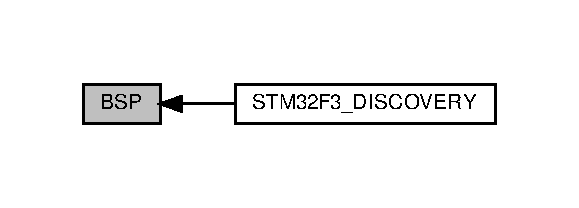
\includegraphics[width=278pt]{group__BSP}
\end{center}
\end{figure}
\subsection*{Modules}
\begin{DoxyCompactItemize}
\item 
\hyperlink{group__STM32F3__DISCOVERY}{S\+T\+M32\+F3\+\_\+\+D\+I\+S\+C\+O\+V\+E\+RY}
\begin{DoxyCompactList}\small\item\em This file provides set of firmware functions to manage Leds and push-\/button available on S\+T\+M32\+F3-\/\+Discovery Kit from S\+T\+Microelectronics. \end{DoxyCompactList}\end{DoxyCompactItemize}


\subsection{Detailed Description}

\hypertarget{group__STM32F3__DISCOVERY}{}\section{S\+T\+M32\+F3\+\_\+\+D\+I\+S\+C\+O\+V\+E\+RY}
\label{group__STM32F3__DISCOVERY}\index{S\+T\+M32\+F3\+\_\+\+D\+I\+S\+C\+O\+V\+E\+RY@{S\+T\+M32\+F3\+\_\+\+D\+I\+S\+C\+O\+V\+E\+RY}}


This file provides set of firmware functions to manage Leds and push-\/button available on S\+T\+M32\+F3-\/\+Discovery Kit from S\+T\+Microelectronics.  


Collaboration diagram for S\+T\+M32\+F3\+\_\+\+D\+I\+S\+C\+O\+V\+E\+RY\+:\nopagebreak
\begin{figure}[H]
\begin{center}
\leavevmode
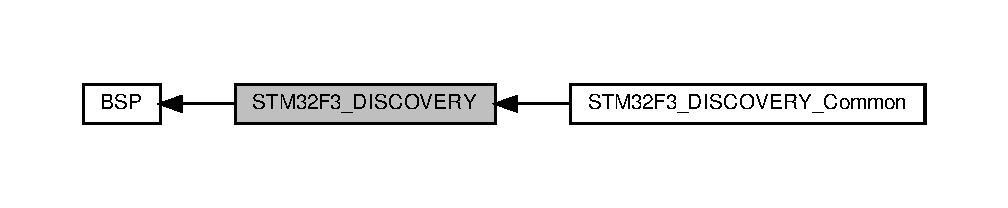
\includegraphics[width=350pt]{group__STM32F3__DISCOVERY}
\end{center}
\end{figure}
\subsection*{Modules}
\begin{DoxyCompactItemize}
\item 
\hyperlink{group__STM32F3__DISCOVERY__Common}{S\+T\+M32\+F3\+\_\+\+D\+I\+S\+C\+O\+V\+E\+R\+Y\+\_\+\+Common}
\end{DoxyCompactItemize}


\subsection{Detailed Description}
This file provides set of firmware functions to manage Leds and push-\/button available on S\+T\+M32\+F3-\/\+Discovery Kit from S\+T\+Microelectronics. 


\hypertarget{group__STM32F3__DISCOVERY__Common}{}\section{S\+T\+M32\+F3\+\_\+\+D\+I\+S\+C\+O\+V\+E\+R\+Y\+\_\+\+Common}
\label{group__STM32F3__DISCOVERY__Common}\index{S\+T\+M32\+F3\+\_\+\+D\+I\+S\+C\+O\+V\+E\+R\+Y\+\_\+\+Common@{S\+T\+M32\+F3\+\_\+\+D\+I\+S\+C\+O\+V\+E\+R\+Y\+\_\+\+Common}}
Collaboration diagram for S\+T\+M32\+F3\+\_\+\+D\+I\+S\+C\+O\+V\+E\+R\+Y\+\_\+\+Common\+:\nopagebreak
\begin{figure}[H]
\begin{center}
\leavevmode
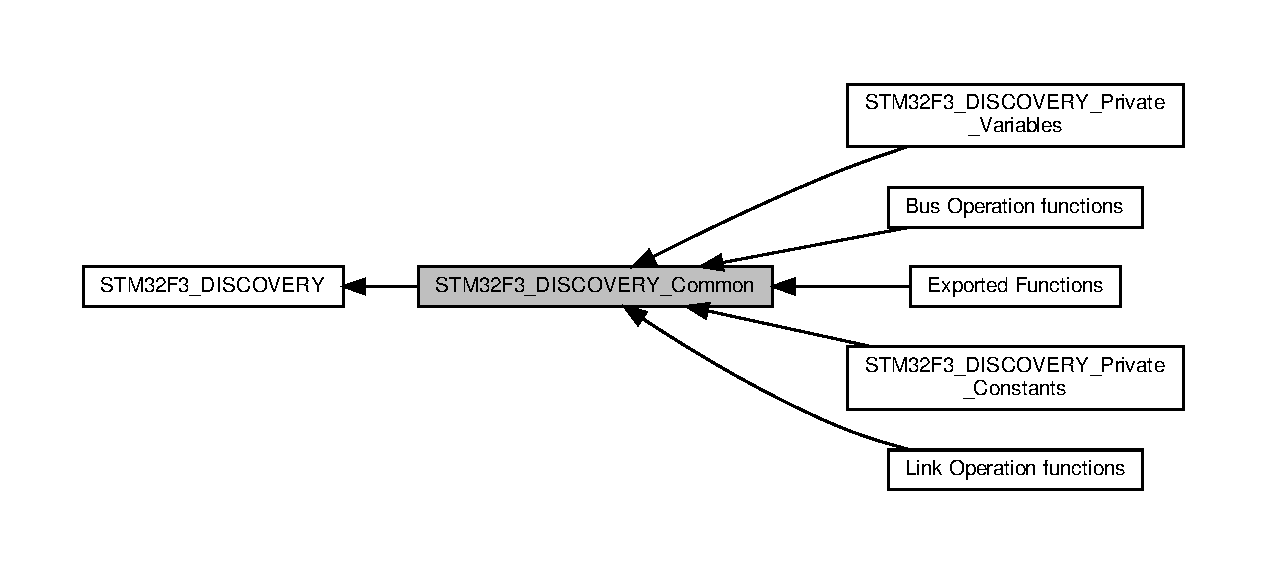
\includegraphics[width=350pt]{group__STM32F3__DISCOVERY__Common}
\end{center}
\end{figure}
\subsection*{Modules}
\begin{DoxyCompactItemize}
\item 
\hyperlink{group__STM32F3__DISCOVERY__BUS}{Bus Operation functions}
\item 
\hyperlink{group__STM32F3__DISCOVERY__LINK__OPERATIONS}{Link Operation functions}
\item 
\hyperlink{group__STM32F3__DISCOVERY__Private__Constants}{S\+T\+M32\+F3\+\_\+\+D\+I\+S\+C\+O\+V\+E\+R\+Y\+\_\+\+Private\+\_\+\+Constants}
\item 
\hyperlink{group__STM32F3__DISCOVERY__Private__Variables}{S\+T\+M32\+F3\+\_\+\+D\+I\+S\+C\+O\+V\+E\+R\+Y\+\_\+\+Private\+\_\+\+Variables}
\item 
\hyperlink{group__STM32F3__DISCOVERY__Exported__Functions}{Exported Functions}
\end{DoxyCompactItemize}


\subsection{Detailed Description}

\hypertarget{group__STM32F3__DISCOVERY__Private__Constants}{}\section{S\+T\+M32\+F3\+\_\+\+D\+I\+S\+C\+O\+V\+E\+R\+Y\+\_\+\+Private\+\_\+\+Constants}
\label{group__STM32F3__DISCOVERY__Private__Constants}\index{S\+T\+M32\+F3\+\_\+\+D\+I\+S\+C\+O\+V\+E\+R\+Y\+\_\+\+Private\+\_\+\+Constants@{S\+T\+M32\+F3\+\_\+\+D\+I\+S\+C\+O\+V\+E\+R\+Y\+\_\+\+Private\+\_\+\+Constants}}
Collaboration diagram for S\+T\+M32\+F3\+\_\+\+D\+I\+S\+C\+O\+V\+E\+R\+Y\+\_\+\+Private\+\_\+\+Constants\+:\nopagebreak
\begin{figure}[H]
\begin{center}
\leavevmode
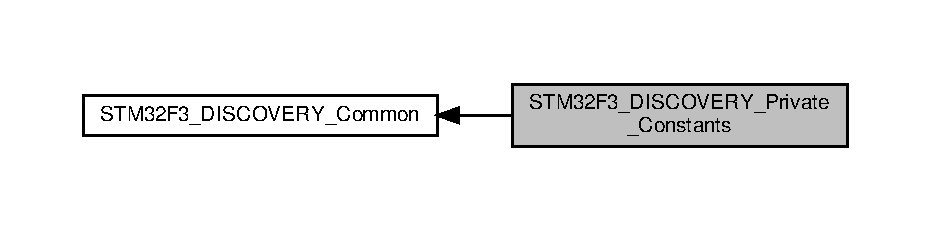
\includegraphics[width=350pt]{group__STM32F3__DISCOVERY__Private__Constants}
\end{center}
\end{figure}

\hypertarget{group__STM32F3__DISCOVERY__Private__Variables}{}\section{S\+T\+M32\+F3\+\_\+\+D\+I\+S\+C\+O\+V\+E\+R\+Y\+\_\+\+Private\+\_\+\+Variables}
\label{group__STM32F3__DISCOVERY__Private__Variables}\index{S\+T\+M32\+F3\+\_\+\+D\+I\+S\+C\+O\+V\+E\+R\+Y\+\_\+\+Private\+\_\+\+Variables@{S\+T\+M32\+F3\+\_\+\+D\+I\+S\+C\+O\+V\+E\+R\+Y\+\_\+\+Private\+\_\+\+Variables}}
Collaboration diagram for S\+T\+M32\+F3\+\_\+\+D\+I\+S\+C\+O\+V\+E\+R\+Y\+\_\+\+Private\+\_\+\+Variables\+:\nopagebreak
\begin{figure}[H]
\begin{center}
\leavevmode
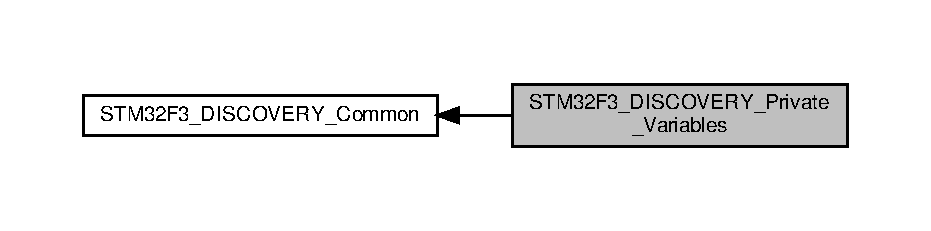
\includegraphics[width=350pt]{group__STM32F3__DISCOVERY__Private__Variables}
\end{center}
\end{figure}


\subsection{Detailed Description}


\subsection{Variable Documentation}
\mbox{\Hypertarget{group__STM32F3__DISCOVERY__Private__Variables_ga51722a2d3aff3970f123a94ac62b908f}\label{group__STM32F3__DISCOVERY__Private__Variables_ga51722a2d3aff3970f123a94ac62b908f}} 
\index{S\+T\+M32\+F3\+\_\+\+D\+I\+S\+C\+O\+V\+E\+R\+Y\+\_\+\+Private\+\_\+\+Variables@{S\+T\+M32\+F3\+\_\+\+D\+I\+S\+C\+O\+V\+E\+R\+Y\+\_\+\+Private\+\_\+\+Variables}!L\+E\+D\+\_\+\+P\+IN@{L\+E\+D\+\_\+\+P\+IN}}
\index{L\+E\+D\+\_\+\+P\+IN@{L\+E\+D\+\_\+\+P\+IN}!S\+T\+M32\+F3\+\_\+\+D\+I\+S\+C\+O\+V\+E\+R\+Y\+\_\+\+Private\+\_\+\+Variables@{S\+T\+M32\+F3\+\_\+\+D\+I\+S\+C\+O\+V\+E\+R\+Y\+\_\+\+Private\+\_\+\+Variables}}
\subsubsection{\texorpdfstring{L\+E\+D\+\_\+\+P\+IN}{LED\_PIN}}
{\footnotesize\ttfamily const uint16\+\_\+t L\+E\+D\+\_\+\+P\+IN\mbox{[}L\+E\+Dn\mbox{]}}

{\bfseries Initial value\+:}
\begin{DoxyCode}
= \{LED3\_PIN, LED4\_PIN, LED5\_PIN, LED6\_PIN,
                                 LED7\_PIN, LED8\_PIN, LED9\_PIN, LED10\_PIN\}
\end{DoxyCode}
\mbox{\Hypertarget{group__STM32F3__DISCOVERY__Private__Variables_ga1127c0cf12e4ec7a66f2a64cd7407218}\label{group__STM32F3__DISCOVERY__Private__Variables_ga1127c0cf12e4ec7a66f2a64cd7407218}} 
\index{S\+T\+M32\+F3\+\_\+\+D\+I\+S\+C\+O\+V\+E\+R\+Y\+\_\+\+Private\+\_\+\+Variables@{S\+T\+M32\+F3\+\_\+\+D\+I\+S\+C\+O\+V\+E\+R\+Y\+\_\+\+Private\+\_\+\+Variables}!L\+E\+D\+\_\+\+P\+O\+RT@{L\+E\+D\+\_\+\+P\+O\+RT}}
\index{L\+E\+D\+\_\+\+P\+O\+RT@{L\+E\+D\+\_\+\+P\+O\+RT}!S\+T\+M32\+F3\+\_\+\+D\+I\+S\+C\+O\+V\+E\+R\+Y\+\_\+\+Private\+\_\+\+Variables@{S\+T\+M32\+F3\+\_\+\+D\+I\+S\+C\+O\+V\+E\+R\+Y\+\_\+\+Private\+\_\+\+Variables}}
\subsubsection{\texorpdfstring{L\+E\+D\+\_\+\+P\+O\+RT}{LED\_PORT}}
{\footnotesize\ttfamily G\+P\+I\+O\+\_\+\+Type\+Def$\ast$ L\+E\+D\+\_\+\+P\+O\+RT\mbox{[}L\+E\+Dn\mbox{]}}

{\bfseries Initial value\+:}
\begin{DoxyCode}
= \{LED3\_GPIO\_PORT, LED4\_GPIO\_PORT, LED5\_GPIO\_PORT, LED6\_GPIO\_PORT,
                                 LED7\_GPIO\_PORT, LED8\_GPIO\_PORT, LED9\_GPIO\_PORT, LED10\_GPIO\_PORT\}
\end{DoxyCode}


L\+ED variables. 


\hypertarget{group__CMSIS}{}\section{C\+M\+S\+IS}
\label{group__CMSIS}\index{C\+M\+S\+IS@{C\+M\+S\+IS}}
Collaboration diagram for C\+M\+S\+IS\+:\nopagebreak
\begin{figure}[H]
\begin{center}
\leavevmode
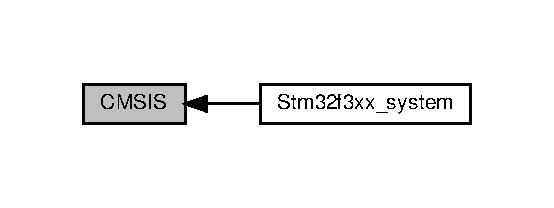
\includegraphics[width=266pt]{group__CMSIS}
\end{center}
\end{figure}
\subsection*{Modules}
\begin{DoxyCompactItemize}
\item 
\hyperlink{group__stm32f3xx__system}{Stm32f3xx\+\_\+system}
\end{DoxyCompactItemize}


\subsection{Detailed Description}

\hypertarget{group__stm32f3xx__system}{}\section{Stm32f3xx\+\_\+system}
\label{group__stm32f3xx__system}\index{Stm32f3xx\+\_\+system@{Stm32f3xx\+\_\+system}}
Collaboration diagram for Stm32f3xx\+\_\+system\+:\nopagebreak
\begin{figure}[H]
\begin{center}
\leavevmode
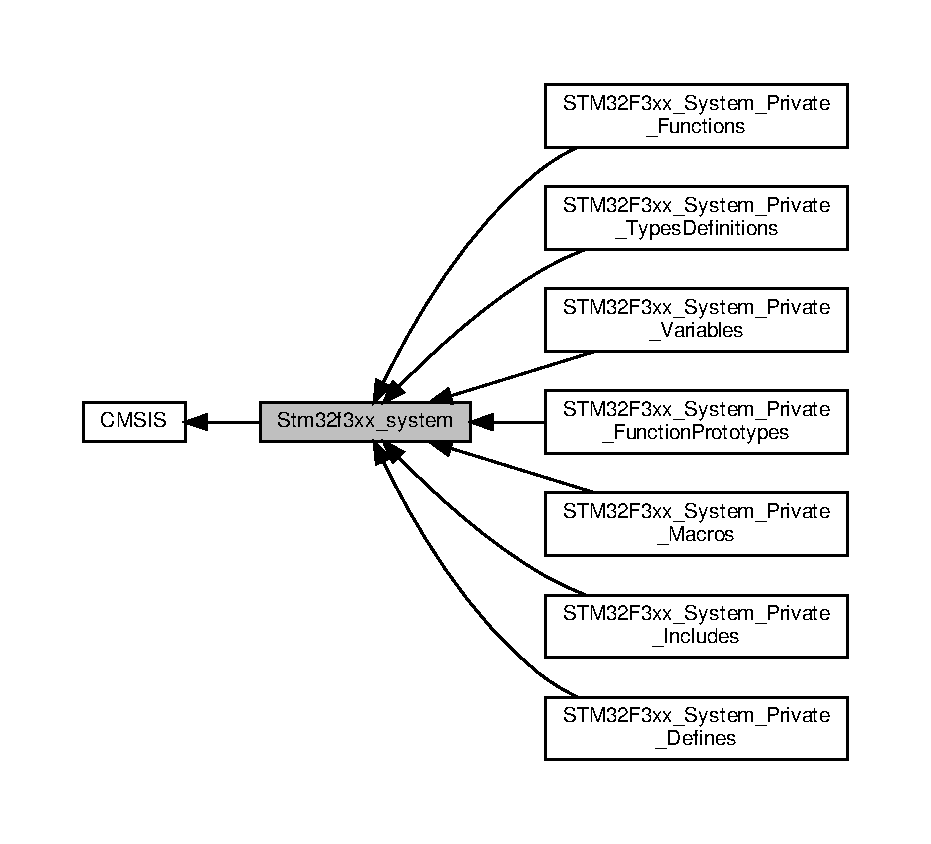
\includegraphics[width=350pt]{group__stm32f3xx__system}
\end{center}
\end{figure}
\subsection*{Modules}
\begin{DoxyCompactItemize}
\item 
\hyperlink{group__STM32F3xx__System__Private__Includes}{S\+T\+M32\+F3xx\+\_\+\+System\+\_\+\+Private\+\_\+\+Includes}
\item 
\hyperlink{group__STM32F3xx__System__Private__TypesDefinitions}{S\+T\+M32\+F3xx\+\_\+\+System\+\_\+\+Private\+\_\+\+Types\+Definitions}
\item 
\hyperlink{group__STM32F3xx__System__Private__Defines}{S\+T\+M32\+F3xx\+\_\+\+System\+\_\+\+Private\+\_\+\+Defines}
\item 
\hyperlink{group__STM32F3xx__System__Private__Macros}{S\+T\+M32\+F3xx\+\_\+\+System\+\_\+\+Private\+\_\+\+Macros}
\item 
\hyperlink{group__STM32F3xx__System__Private__Variables}{S\+T\+M32\+F3xx\+\_\+\+System\+\_\+\+Private\+\_\+\+Variables}
\item 
\hyperlink{group__STM32F3xx__System__Private__FunctionPrototypes}{S\+T\+M32\+F3xx\+\_\+\+System\+\_\+\+Private\+\_\+\+Function\+Prototypes}
\item 
\hyperlink{group__STM32F3xx__System__Private__Functions}{S\+T\+M32\+F3xx\+\_\+\+System\+\_\+\+Private\+\_\+\+Functions}
\end{DoxyCompactItemize}


\subsection{Detailed Description}

\hypertarget{group__STM32F3xx__System__Private__Includes}{}\section{S\+T\+M32\+F3xx\+\_\+\+System\+\_\+\+Private\+\_\+\+Includes}
\label{group__STM32F3xx__System__Private__Includes}\index{S\+T\+M32\+F3xx\+\_\+\+System\+\_\+\+Private\+\_\+\+Includes@{S\+T\+M32\+F3xx\+\_\+\+System\+\_\+\+Private\+\_\+\+Includes}}
Collaboration diagram for S\+T\+M32\+F3xx\+\_\+\+System\+\_\+\+Private\+\_\+\+Includes\+:\nopagebreak
\begin{figure}[H]
\begin{center}
\leavevmode
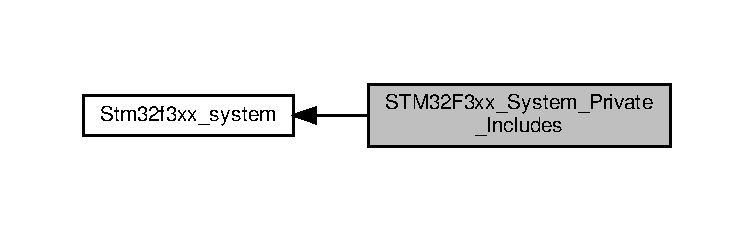
\includegraphics[width=350pt]{group__STM32F3xx__System__Private__Includes}
\end{center}
\end{figure}

\hypertarget{group__STM32F3xx__System__Private__TypesDefinitions}{}\section{S\+T\+M32\+F3xx\+\_\+\+System\+\_\+\+Private\+\_\+\+Types\+Definitions}
\label{group__STM32F3xx__System__Private__TypesDefinitions}\index{S\+T\+M32\+F3xx\+\_\+\+System\+\_\+\+Private\+\_\+\+Types\+Definitions@{S\+T\+M32\+F3xx\+\_\+\+System\+\_\+\+Private\+\_\+\+Types\+Definitions}}
Collaboration diagram for S\+T\+M32\+F3xx\+\_\+\+System\+\_\+\+Private\+\_\+\+Types\+Definitions\+:\nopagebreak
\begin{figure}[H]
\begin{center}
\leavevmode
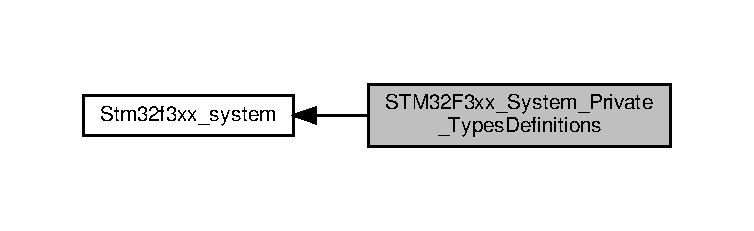
\includegraphics[width=350pt]{group__STM32F3xx__System__Private__TypesDefinitions}
\end{center}
\end{figure}

\hypertarget{group__STM32F3xx__System__Private__Defines}{}\section{S\+T\+M32\+F3xx\+\_\+\+System\+\_\+\+Private\+\_\+\+Defines}
\label{group__STM32F3xx__System__Private__Defines}\index{S\+T\+M32\+F3xx\+\_\+\+System\+\_\+\+Private\+\_\+\+Defines@{S\+T\+M32\+F3xx\+\_\+\+System\+\_\+\+Private\+\_\+\+Defines}}
Collaboration diagram for S\+T\+M32\+F3xx\+\_\+\+System\+\_\+\+Private\+\_\+\+Defines\+:\nopagebreak
\begin{figure}[H]
\begin{center}
\leavevmode
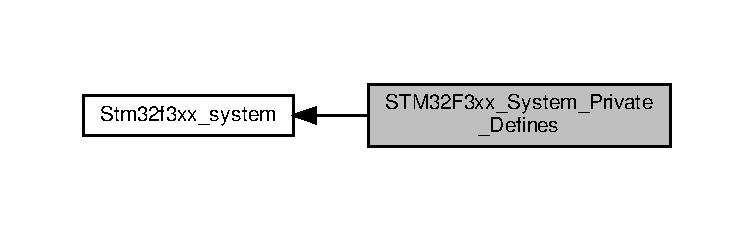
\includegraphics[width=350pt]{group__STM32F3xx__System__Private__Defines}
\end{center}
\end{figure}

\hypertarget{group__STM32F3xx__System__Private__Macros}{}\section{S\+T\+M32\+F3xx\+\_\+\+System\+\_\+\+Private\+\_\+\+Macros}
\label{group__STM32F3xx__System__Private__Macros}\index{S\+T\+M32\+F3xx\+\_\+\+System\+\_\+\+Private\+\_\+\+Macros@{S\+T\+M32\+F3xx\+\_\+\+System\+\_\+\+Private\+\_\+\+Macros}}
Collaboration diagram for S\+T\+M32\+F3xx\+\_\+\+System\+\_\+\+Private\+\_\+\+Macros\+:\nopagebreak
\begin{figure}[H]
\begin{center}
\leavevmode
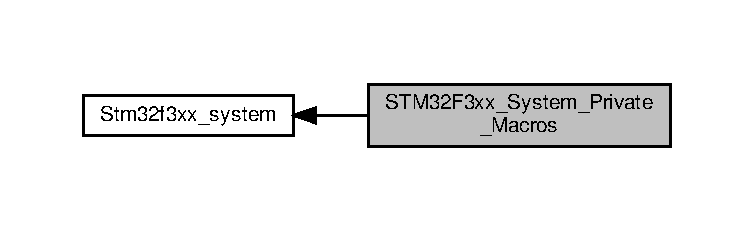
\includegraphics[width=350pt]{group__STM32F3xx__System__Private__Macros}
\end{center}
\end{figure}

\hypertarget{group__STM32F3xx__System__Private__Variables}{}\section{S\+T\+M32\+F3xx\+\_\+\+System\+\_\+\+Private\+\_\+\+Variables}
\label{group__STM32F3xx__System__Private__Variables}\index{S\+T\+M32\+F3xx\+\_\+\+System\+\_\+\+Private\+\_\+\+Variables@{S\+T\+M32\+F3xx\+\_\+\+System\+\_\+\+Private\+\_\+\+Variables}}
Collaboration diagram for S\+T\+M32\+F3xx\+\_\+\+System\+\_\+\+Private\+\_\+\+Variables\+:\nopagebreak
\begin{figure}[H]
\begin{center}
\leavevmode
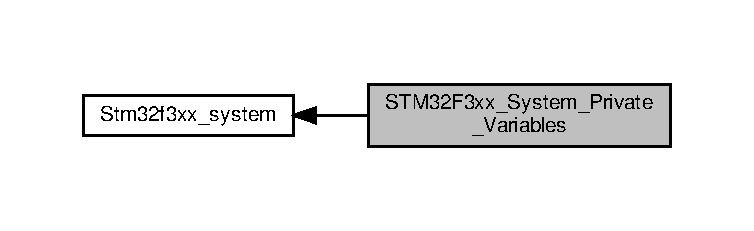
\includegraphics[width=350pt]{group__STM32F3xx__System__Private__Variables}
\end{center}
\end{figure}


\subsection{Detailed Description}

\hypertarget{group__STM32F3xx__System__Private__FunctionPrototypes}{}\section{S\+T\+M32\+F3xx\+\_\+\+System\+\_\+\+Private\+\_\+\+Function\+Prototypes}
\label{group__STM32F3xx__System__Private__FunctionPrototypes}\index{S\+T\+M32\+F3xx\+\_\+\+System\+\_\+\+Private\+\_\+\+Function\+Prototypes@{S\+T\+M32\+F3xx\+\_\+\+System\+\_\+\+Private\+\_\+\+Function\+Prototypes}}
Collaboration diagram for S\+T\+M32\+F3xx\+\_\+\+System\+\_\+\+Private\+\_\+\+Function\+Prototypes\+:\nopagebreak
\begin{figure}[H]
\begin{center}
\leavevmode
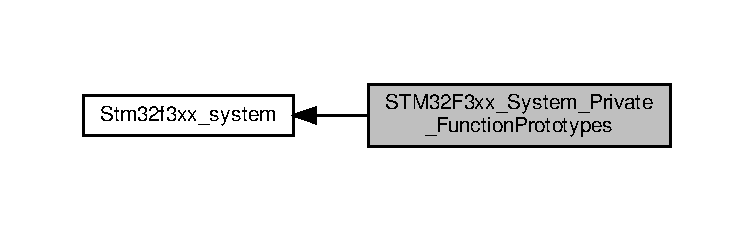
\includegraphics[width=350pt]{group__STM32F3xx__System__Private__FunctionPrototypes}
\end{center}
\end{figure}

\hypertarget{group__STM32F3xx__System__Private__Functions}{}\section{S\+T\+M32\+F3xx\+\_\+\+System\+\_\+\+Private\+\_\+\+Functions}
\label{group__STM32F3xx__System__Private__Functions}\index{S\+T\+M32\+F3xx\+\_\+\+System\+\_\+\+Private\+\_\+\+Functions@{S\+T\+M32\+F3xx\+\_\+\+System\+\_\+\+Private\+\_\+\+Functions}}
Collaboration diagram for S\+T\+M32\+F3xx\+\_\+\+System\+\_\+\+Private\+\_\+\+Functions\+:\nopagebreak
\begin{figure}[H]
\begin{center}
\leavevmode
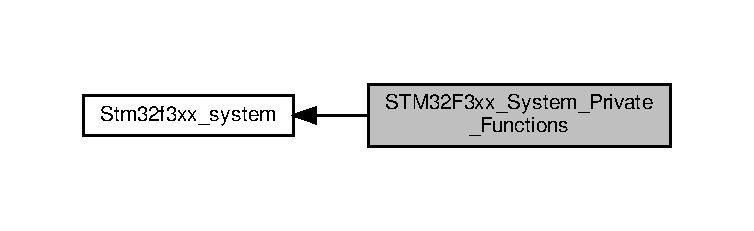
\includegraphics[width=350pt]{group__STM32F3xx__System__Private__Functions}
\end{center}
\end{figure}


\subsection{Detailed Description}


\subsection{Function Documentation}
\mbox{\Hypertarget{group__STM32F3xx__System__Private__Functions_ga19a0c3ef7421e9045e62d7df7f1120a9}\label{group__STM32F3xx__System__Private__Functions_ga19a0c3ef7421e9045e62d7df7f1120a9}} 
\index{S\+T\+M32\+F3xx\+\_\+\+System\+\_\+\+Private\+\_\+\+Functions@{S\+T\+M32\+F3xx\+\_\+\+System\+\_\+\+Private\+\_\+\+Functions}!System\+Core\+Clock\+Update@{System\+Core\+Clock\+Update}}
\index{System\+Core\+Clock\+Update@{System\+Core\+Clock\+Update}!S\+T\+M32\+F3xx\+\_\+\+System\+\_\+\+Private\+\_\+\+Functions@{S\+T\+M32\+F3xx\+\_\+\+System\+\_\+\+Private\+\_\+\+Functions}}
\subsubsection{\texorpdfstring{System\+Core\+Clock\+Update()}{SystemCoreClockUpdate()}}
{\footnotesize\ttfamily void System\+Core\+Clock\+Update (\begin{DoxyParamCaption}\item[{void}]{ }\end{DoxyParamCaption})}



Update System\+Core\+Clock variable according to Clock Register Values. The System\+Core\+Clock variable contains the core clock (H\+C\+LK), it can be used by the user application to setup the Sys\+Tick timer or configure other parameters. 

\begin{DoxyNote}{Note}
Each time the core clock (H\+C\+LK) changes, this function must be called to update System\+Core\+Clock variable value. Otherwise, any configuration based on this variable will be incorrect.

-\/ The system frequency computed by this function is not the real frequency in the chip. It is calculated based on the predefined constant and the selected clock source\+:
\end{DoxyNote}

\begin{DoxyItemize}
\item If S\+Y\+S\+C\+LK source is H\+SI, System\+Core\+Clock will contain the H\+S\+I\+\_\+\+V\+A\+L\+U\+E($\ast$)
\item If S\+Y\+S\+C\+LK source is H\+SE, System\+Core\+Clock will contain the H\+S\+E\+\_\+\+V\+A\+L\+U\+E($\ast$$\ast$)
\item If S\+Y\+S\+C\+LK source is P\+LL, System\+Core\+Clock will contain the H\+S\+E\+\_\+\+V\+A\+L\+U\+E($\ast$$\ast$) or H\+S\+I\+\_\+\+V\+A\+L\+U\+E($\ast$) multiplied/divided by the P\+LL factors.
\end{DoxyItemize}

($\ast$) H\+S\+I\+\_\+\+V\+A\+L\+UE is a constant defined in stm32f3xx\+\_\+hal.\+h file (default value 8 M\+Hz) but the real value may vary depending on the variations in voltage and temperature.

($\ast$$\ast$) H\+S\+E\+\_\+\+V\+A\+L\+UE is a constant defined in stm32f3xx\+\_\+hal.\+h file (default value 8 M\+Hz), user has to ensure that H\+S\+E\+\_\+\+V\+A\+L\+UE is same as the real frequency of the crystal used. Otherwise, this function may have wrong result.


\begin{DoxyItemize}
\item The result of this function could be not correct when using fractional value for H\+SE crystal.
\end{DoxyItemize}


\begin{DoxyParams}{Parameters}
{\em None} & \\
\hline
\end{DoxyParams}

\begin{DoxyRetVals}{Return values}
{\em None} & \\
\hline
\end{DoxyRetVals}
\mbox{\Hypertarget{group__STM32F3xx__System__Private__Functions_gaf019145746f780cda3053023bd6c1819}\label{group__STM32F3xx__System__Private__Functions_gaf019145746f780cda3053023bd6c1819}} 
\index{S\+T\+M32\+F3xx\+\_\+\+System\+\_\+\+Private\+\_\+\+Functions@{S\+T\+M32\+F3xx\+\_\+\+System\+\_\+\+Private\+\_\+\+Functions}!System\+Init@{System\+Init}}
\index{System\+Init@{System\+Init}!S\+T\+M32\+F3xx\+\_\+\+System\+\_\+\+Private\+\_\+\+Functions@{S\+T\+M32\+F3xx\+\_\+\+System\+\_\+\+Private\+\_\+\+Functions}}
\subsubsection{\texorpdfstring{System\+Init()}{SystemInit()}}
{\footnotesize\ttfamily void System\+Init (\begin{DoxyParamCaption}\item[{void}]{ }\end{DoxyParamCaption})}



Setup the microcontroller system Initialize the F\+PU setting, vector table location and the P\+LL configuration is reset. 


\begin{DoxyParams}{Parameters}
{\em None} & \\
\hline
\end{DoxyParams}

\begin{DoxyRetVals}{Return values}
{\em None} & \\
\hline
\end{DoxyRetVals}

\chapter{Data Structure Documentation}
\hypertarget{classGPIO__v1__0_1_1arch__imp}{}\section{arch\+\_\+imp Architecture Reference}
\label{classGPIO__v1__0_1_1arch__imp}\index{arch\+\_\+imp@{arch\+\_\+imp}}
\subsection*{Components}
 \begin{DoxyCompactItemize}
\item 
\mbox{\Hypertarget{classGPIO__v1__0_1_1arch__imp_acfa88fcc633c72af8bfd7e652932f7c7}\label{classGPIO__v1__0_1_1arch__imp_acfa88fcc633c72af8bfd7e652932f7c7}} 
\hyperlink{classGPIO__v1__0_1_1arch__imp_acfa88fcc633c72af8bfd7e652932f7c7}{G\+P\+I\+O\+\_\+v1\+\_\+0\+\_\+\+S00\+\_\+\+A\+XI}  {\bfseries }  
\end{DoxyCompactItemize}
\subsection*{Instantiations}
 \begin{DoxyCompactItemize}
\item 
\mbox{\Hypertarget{classGPIO__v1__0_1_1arch__imp_add7a292f6a3530426561c0d1bf9540b4}\label{classGPIO__v1__0_1_1arch__imp_add7a292f6a3530426561c0d1bf9540b4}} 
\hyperlink{classGPIO__v1__0_1_1arch__imp_add7a292f6a3530426561c0d1bf9540b4}{gpio\+\_\+v1\+\_\+0\+\_\+s00\+\_\+axi\+\_\+inst}  {\bfseries G\+P\+I\+O\+\_\+v1\+\_\+0\+\_\+\+S00\+\_\+\+A\+XI}   
\end{DoxyCompactItemize}


The documentation for this class was generated from the following file\+:\begin{DoxyCompactItemize}
\item 
/media/saverio/\+O\+S/\+Users/\+Saverio/\+Desktop/\+S\+E/git/\+Andrea/\+F\+P\+G\+A/ip\+\_\+repo/\+G\+P\+I\+O\+\_\+1.\+0/hdl/\hyperlink{GPIO__v1__0_8vhd}{G\+P\+I\+O\+\_\+v1\+\_\+0.\+vhd}\end{DoxyCompactItemize}

\hypertarget{classUART__v1__0_1_1arch__imp}{}\section{arch\+\_\+imp Architecture Reference}
\label{classUART__v1__0_1_1arch__imp}\index{arch\+\_\+imp@{arch\+\_\+imp}}


componente U\+A\+R\+T\+\_\+\+A\+X\+I\+\_\+\+S00  componente nel quale è incapsulato il componente \hyperlink{structUART}{U\+A\+RT} e la logica di gestione delle interruzioni.  


\subsection*{Components}
 \begin{DoxyCompactItemize}
\item 
\mbox{\Hypertarget{classUART__v1__0_1_1arch__imp_a554bf35242758ea2c6cdb41b3a146b89}\label{classUART__v1__0_1_1arch__imp_a554bf35242758ea2c6cdb41b3a146b89}} 
\hyperlink{classUART__v1__0_1_1arch__imp_a554bf35242758ea2c6cdb41b3a146b89}{U\+A\+R\+T\+\_\+v1\+\_\+0\+\_\+\+S00\+\_\+\+A\+XI}  {\bfseries }  
\end{DoxyCompactItemize}
\subsection*{Instantiations}
 \begin{DoxyCompactItemize}
\item 
\mbox{\Hypertarget{classUART__v1__0_1_1arch__imp_af8995827bb89a3b54bf57d79330e4cf5}\label{classUART__v1__0_1_1arch__imp_af8995827bb89a3b54bf57d79330e4cf5}} 
\hyperlink{classUART__v1__0_1_1arch__imp_af8995827bb89a3b54bf57d79330e4cf5}{uart\+\_\+v1\+\_\+0\+\_\+s00\+\_\+axi\+\_\+inst}  {\bfseries U\+A\+R\+T\+\_\+v1\+\_\+0\+\_\+\+S00\+\_\+\+A\+XI}   
\end{DoxyCompactItemize}


\subsection{Detailed Description}
componente U\+A\+R\+T\+\_\+\+A\+X\+I\+\_\+\+S00  componente nel quale è incapsulato il componente \hyperlink{structUART}{U\+A\+RT} e la logica di gestione delle interruzioni. 

The documentation for this class was generated from the following file\+:\begin{DoxyCompactItemize}
\item 
/media/saverio/\+O\+S/\+Users/\+Saverio/\+Desktop/\+S\+E/git/codici\+\_\+da\+\_\+mandare/\+F\+P\+G\+A/\+U\+A\+R\+T/\+Hardware/\+U\+A\+R\+T\+\_\+1.\+0/hdl/\hyperlink{UART__v1__0_8vhd}{U\+A\+R\+T\+\_\+v1\+\_\+0.\+vhd}\end{DoxyCompactItemize}

\hypertarget{classUART__v1__0__S00__AXI_1_1arch__imp}{}\section{arch\+\_\+imp Architecture Reference}
\label{classUART__v1__0__S00__AXI_1_1arch__imp}\index{arch\+\_\+imp@{arch\+\_\+imp}}
\subsection*{Processes}
 \begin{DoxyCompactItemize}
\item 
\mbox{\Hypertarget{classUART__v1__0__S00__AXI_1_1arch__imp_a3bd49952c6361256b0fd16de71d09227}\label{classUART__v1__0__S00__AXI_1_1arch__imp_a3bd49952c6361256b0fd16de71d09227}} 
\hyperlink{classUART__v1__0__S00__AXI_1_1arch__imp_a3bd49952c6361256b0fd16de71d09227}{P\+R\+O\+C\+E\+S\+S\+\_\+9}{\bfseries  ( {\bfseries \textcolor{vhdlchar}{S\+\_\+\+A\+X\+I\+\_\+\+A\+C\+LK}\textcolor{vhdlchar}{ }} )}
\begin{DoxyCompactList}\small\item\em dato ricevuto \end{DoxyCompactList}\item 
\mbox{\Hypertarget{classUART__v1__0__S00__AXI_1_1arch__imp_a8fbd1d135ff76bf9241c19565ede6f47}\label{classUART__v1__0__S00__AXI_1_1arch__imp_a8fbd1d135ff76bf9241c19565ede6f47}} 
\hyperlink{classUART__v1__0__S00__AXI_1_1arch__imp_a8fbd1d135ff76bf9241c19565ede6f47}{P\+R\+O\+C\+E\+S\+S\+\_\+10}{\bfseries  ( {\bfseries \textcolor{vhdlchar}{S\+\_\+\+A\+X\+I\+\_\+\+A\+C\+LK}\textcolor{vhdlchar}{ }} )}
\begin{DoxyCompactList}\small\item\em segnale il cui valore alto indica che un nuovo dato ricevuto è dispobile \end{DoxyCompactList}\item 
\mbox{\Hypertarget{classUART__v1__0__S00__AXI_1_1arch__imp_a86849bc293eedede60c3794d52db5cf2}\label{classUART__v1__0__S00__AXI_1_1arch__imp_a86849bc293eedede60c3794d52db5cf2}} 
\hyperlink{classUART__v1__0__S00__AXI_1_1arch__imp_a86849bc293eedede60c3794d52db5cf2}{P\+R\+O\+C\+E\+S\+S\+\_\+11}{\bfseries  ( {\bfseries \textcolor{vhdlchar}{S\+\_\+\+A\+X\+I\+\_\+\+A\+C\+LK}\textcolor{vhdlchar}{ }} )}
\item 
\mbox{\Hypertarget{classUART__v1__0__S00__AXI_1_1arch__imp_acf9a8d423319c94928908546cd66d779}\label{classUART__v1__0__S00__AXI_1_1arch__imp_acf9a8d423319c94928908546cd66d779}} 
\hyperlink{classUART__v1__0__S00__AXI_1_1arch__imp_acf9a8d423319c94928908546cd66d779}{P\+R\+O\+C\+E\+S\+S\+\_\+12}{\bfseries  ( {\bfseries \textcolor{vhdlchar}{S\+\_\+\+A\+X\+I\+\_\+\+A\+C\+LK}\textcolor{vhdlchar}{ }} )}
\item 
\mbox{\Hypertarget{classUART__v1__0__S00__AXI_1_1arch__imp_a46ef74882494d566c9af5b92859df7f8}\label{classUART__v1__0__S00__AXI_1_1arch__imp_a46ef74882494d566c9af5b92859df7f8}} 
\hyperlink{classUART__v1__0__S00__AXI_1_1arch__imp_a46ef74882494d566c9af5b92859df7f8}{P\+R\+O\+C\+E\+S\+S\+\_\+13}{\bfseries  ( {\bfseries \textcolor{vhdlchar}{S\+\_\+\+A\+X\+I\+\_\+\+A\+C\+LK}\textcolor{vhdlchar}{ }} )}
\item 
\mbox{\Hypertarget{classUART__v1__0__S00__AXI_1_1arch__imp_a540733a9d881f3739d4b074f82493696}\label{classUART__v1__0__S00__AXI_1_1arch__imp_a540733a9d881f3739d4b074f82493696}} 
\hyperlink{classUART__v1__0__S00__AXI_1_1arch__imp_a540733a9d881f3739d4b074f82493696}{P\+R\+O\+C\+E\+S\+S\+\_\+14}{\bfseries  ( {\bfseries \textcolor{vhdlchar}{S\+\_\+\+A\+X\+I\+\_\+\+A\+C\+LK}\textcolor{vhdlchar}{ }} )}
\item 
\mbox{\Hypertarget{classUART__v1__0__S00__AXI_1_1arch__imp_af63a9d34999cb0a12e3012f5d6afbbfc}\label{classUART__v1__0__S00__AXI_1_1arch__imp_af63a9d34999cb0a12e3012f5d6afbbfc}} 
\hyperlink{classUART__v1__0__S00__AXI_1_1arch__imp_af63a9d34999cb0a12e3012f5d6afbbfc}{P\+R\+O\+C\+E\+S\+S\+\_\+15}{\bfseries  ( {\bfseries \textcolor{vhdlchar}{S\+\_\+\+A\+X\+I\+\_\+\+A\+C\+LK}\textcolor{vhdlchar}{ }} )}
\item 
\mbox{\Hypertarget{classUART__v1__0__S00__AXI_1_1arch__imp_ac00102850623a2fb02531f06a51c6401}\label{classUART__v1__0__S00__AXI_1_1arch__imp_ac00102850623a2fb02531f06a51c6401}} 
\hyperlink{classUART__v1__0__S00__AXI_1_1arch__imp_ac00102850623a2fb02531f06a51c6401}{P\+R\+O\+C\+E\+S\+S\+\_\+16}{\bfseries  ( {\bfseries \textcolor{vhdlchar}{slv\+\_\+reg0}\textcolor{vhdlchar}{ }} , {\bfseries \textcolor{vhdlchar}{slv\+\_\+reg1}\textcolor{vhdlchar}{ }} , {\bfseries \textcolor{vhdlchar}{uart\+\_\+status\+\_\+reg}\textcolor{vhdlchar}{ }} , {\bfseries \textcolor{vhdlchar}{slv\+\_\+reg3\+\_\+out}\textcolor{vhdlchar}{ }} , {\bfseries \textcolor{vhdlchar}{slv\+\_\+reg4}\textcolor{vhdlchar}{ }} , {\bfseries \textcolor{vhdlchar}{slv\+\_\+reg5}\textcolor{vhdlchar}{ }} , {\bfseries \textcolor{vhdlchar}{slv\+\_\+reg6}\textcolor{vhdlchar}{ }} , {\bfseries \textcolor{vhdlchar}{slv\+\_\+reg7\+\_\+out}\textcolor{vhdlchar}{ }} , {\bfseries \textcolor{vhdlchar}{axi\+\_\+araddr}\textcolor{vhdlchar}{ }} , {\bfseries \textcolor{vhdlchar}{S\+\_\+\+A\+X\+I\+\_\+\+A\+R\+E\+S\+E\+TN}\textcolor{vhdlchar}{ }} , {\bfseries \textcolor{vhdlchar}{slv\+\_\+reg\+\_\+rden}\textcolor{vhdlchar}{ }} )}
\item 
\mbox{\Hypertarget{classUART__v1__0__S00__AXI_1_1arch__imp_a6b83b9626c3e03102e58d7d89aad43eb}\label{classUART__v1__0__S00__AXI_1_1arch__imp_a6b83b9626c3e03102e58d7d89aad43eb}} 
\hyperlink{classUART__v1__0__S00__AXI_1_1arch__imp_a6b83b9626c3e03102e58d7d89aad43eb}{P\+R\+O\+C\+E\+S\+S\+\_\+17}{\bfseries  ( {\bfseries \textcolor{vhdlchar}{S\+\_\+\+A\+X\+I\+\_\+\+A\+C\+LK}\textcolor{vhdlchar}{ }} )}
\item 
\hyperlink{classUART__v1__0__S00__AXI_1_1arch__imp_a1c2628d089a3915505bce1cba131c80a}{status\+\_\+reg\+\_\+sampling}{\bfseries  ( {\bfseries \textcolor{vhdlchar}{S\+\_\+\+A\+X\+I\+\_\+\+A\+C\+LK}\textcolor{vhdlchar}{ }} , {\bfseries \textcolor{vhdlchar}{uart\+\_\+status\+\_\+reg}\textcolor{vhdlchar}{ }} )}
\begin{DoxyCompactList}\small\item\em Campiona i segnali di cui si vuole verificare la generazione di un interrupt. \end{DoxyCompactList}\item 
\hyperlink{classUART__v1__0__S00__AXI_1_1arch__imp_a72db935ad9e80a3434cfb113c364c329}{intr\+\_\+pending}{\bfseries  ( {\bfseries \textcolor{vhdlchar}{S\+\_\+\+A\+X\+I\+\_\+\+A\+C\+LK}\textcolor{vhdlchar}{ }} , {\bfseries \textcolor{vhdlchar}{change\+\_\+detected}\textcolor{vhdlchar}{ }} , {\bfseries {\bfseries \hyperlink{classUART__v1__0__S00__AXI_1_1arch__imp_a65e0e54a6d565935dd24ce96dbbce53a}{ack\+\_\+intr}} \textcolor{vhdlchar}{ }} )}
\begin{DoxyCompactList}\small\item\em Gestisce il registro pending. \end{DoxyCompactList}\item 
\hyperlink{classUART__v1__0__S00__AXI_1_1arch__imp_a48d068c63e454a766cd9703aff942fb6}{inst\+\_\+irq}{\bfseries  ( {\bfseries \textcolor{vhdlchar}{S\+\_\+\+A\+X\+I\+\_\+\+A\+C\+LK}\textcolor{vhdlchar}{ }} , {\bfseries {\bfseries \hyperlink{classUART__v1__0__S00__AXI_1_1arch__imp_a5595ca2e548ef1d12b7fa2bac3e2aa00}{pending\+\_\+intr}} \textcolor{vhdlchar}{ }} )}
\begin{DoxyCompactList}\small\item\em Disabilita l\textquotesingle{} interrupt nel caso di reset del bus e tiene alto il segnale di interrupt finchè rimane pendente. \end{DoxyCompactList}\end{DoxyCompactItemize}
\subsection*{Components}
 \begin{DoxyCompactItemize}
\item 
\hyperlink{classUART__v1__0__S00__AXI_1_1arch__imp_a6f88b8988ee3bab3eaaa301212c7f804}{U\+A\+RT}  {\bfseries }  
\begin{DoxyCompactList}\small\item\em U\+A\+RT. \end{DoxyCompactList}\end{DoxyCompactItemize}
\subsection*{Constants}
 \begin{DoxyCompactItemize}
\item 
\mbox{\Hypertarget{classUART__v1__0__S00__AXI_1_1arch__imp_a92f00d1b43f901f1bf5684d1e79aab84}\label{classUART__v1__0__S00__AXI_1_1arch__imp_a92f00d1b43f901f1bf5684d1e79aab84}} 
\hyperlink{classUART__v1__0__S00__AXI_1_1arch__imp_a92f00d1b43f901f1bf5684d1e79aab84}{A\+D\+D\+R\+\_\+\+L\+SB} {\bfseries \textcolor{vhdlchar}{integer}\textcolor{vhdlchar}{ }\textcolor{vhdlchar}{ }\textcolor{vhdlchar}{\+:}\textcolor{vhdlchar}{=}\textcolor{vhdlchar}{ }\textcolor{vhdlchar}{(}\textcolor{vhdlchar}{ }\textcolor{vhdlchar}{ }\textcolor{vhdlchar}{ }\textcolor{vhdlchar}{ }\textcolor{vhdlchar}{C\+\_\+\+S\+\_\+\+A\+X\+I\+\_\+\+D\+A\+T\+A\+\_\+\+W\+I\+D\+TH}\textcolor{vhdlchar}{/}\textcolor{vhdlchar}{ } \textcolor{vhdldigit}{32} \textcolor{vhdlchar}{ }\textcolor{vhdlchar}{)}\textcolor{vhdlchar}{ }\textcolor{vhdlchar}{+}\textcolor{vhdlchar}{ } \textcolor{vhdldigit}{1} \textcolor{vhdlchar}{ }} 
\item 
\mbox{\Hypertarget{classUART__v1__0__S00__AXI_1_1arch__imp_a913a8d777fcc731ba920264a143ec91f}\label{classUART__v1__0__S00__AXI_1_1arch__imp_a913a8d777fcc731ba920264a143ec91f}} 
\hyperlink{classUART__v1__0__S00__AXI_1_1arch__imp_a913a8d777fcc731ba920264a143ec91f}{O\+P\+T\+\_\+\+M\+E\+M\+\_\+\+A\+D\+D\+R\+\_\+\+B\+I\+TS} {\bfseries \textcolor{vhdlchar}{integer}\textcolor{vhdlchar}{ }\textcolor{vhdlchar}{ }\textcolor{vhdlchar}{\+:}\textcolor{vhdlchar}{=}\textcolor{vhdlchar}{ }\textcolor{vhdlchar}{ } \textcolor{vhdldigit}{2} \textcolor{vhdlchar}{ }} 
\end{DoxyCompactItemize}
\subsection*{Signals}
 \begin{DoxyCompactItemize}
\item 
\mbox{\Hypertarget{classUART__v1__0__S00__AXI_1_1arch__imp_ac022af52d7126cf515130cdd10e089fc}\label{classUART__v1__0__S00__AXI_1_1arch__imp_ac022af52d7126cf515130cdd10e089fc}} 
\hyperlink{classUART__v1__0__S00__AXI_1_1arch__imp_ac022af52d7126cf515130cdd10e089fc}{axi\+\_\+awaddr} {\bfseries \textcolor{vhdlchar}{std\+\_\+logic\+\_\+vector}\textcolor{vhdlchar}{ }\textcolor{vhdlchar}{(}\textcolor{vhdlchar}{ }\textcolor{vhdlchar}{ }\textcolor{vhdlchar}{ }\textcolor{vhdlchar}{ }\textcolor{vhdlchar}{C\+\_\+\+S\+\_\+\+A\+X\+I\+\_\+\+A\+D\+D\+R\+\_\+\+W\+I\+D\+TH}\textcolor{vhdlchar}{-\/}\textcolor{vhdlchar}{ } \textcolor{vhdldigit}{1} \textcolor{vhdlchar}{ }\textcolor{vhdlchar}{downto}\textcolor{vhdlchar}{ }\textcolor{vhdlchar}{ } \textcolor{vhdldigit}{0} \textcolor{vhdlchar}{ }\textcolor{vhdlchar}{)}\textcolor{vhdlchar}{ }} 
\item 
\mbox{\Hypertarget{classUART__v1__0__S00__AXI_1_1arch__imp_abe920675e5bffe2b708237782acd713d}\label{classUART__v1__0__S00__AXI_1_1arch__imp_abe920675e5bffe2b708237782acd713d}} 
\hyperlink{classUART__v1__0__S00__AXI_1_1arch__imp_abe920675e5bffe2b708237782acd713d}{axi\+\_\+awready} {\bfseries \textcolor{vhdlchar}{std\+\_\+logic}\textcolor{vhdlchar}{ }} 
\item 
\mbox{\Hypertarget{classUART__v1__0__S00__AXI_1_1arch__imp_a65364960779319dfc2c67e7d943d0499}\label{classUART__v1__0__S00__AXI_1_1arch__imp_a65364960779319dfc2c67e7d943d0499}} 
\hyperlink{classUART__v1__0__S00__AXI_1_1arch__imp_a65364960779319dfc2c67e7d943d0499}{axi\+\_\+wready} {\bfseries \textcolor{vhdlchar}{std\+\_\+logic}\textcolor{vhdlchar}{ }} 
\item 
\mbox{\Hypertarget{classUART__v1__0__S00__AXI_1_1arch__imp_ae5e5ea90e34af927db9507875d261a1a}\label{classUART__v1__0__S00__AXI_1_1arch__imp_ae5e5ea90e34af927db9507875d261a1a}} 
\hyperlink{classUART__v1__0__S00__AXI_1_1arch__imp_ae5e5ea90e34af927db9507875d261a1a}{axi\+\_\+bresp} {\bfseries \textcolor{vhdlchar}{std\+\_\+logic\+\_\+vector}\textcolor{vhdlchar}{ }\textcolor{vhdlchar}{(}\textcolor{vhdlchar}{ }\textcolor{vhdlchar}{ } \textcolor{vhdldigit}{1} \textcolor{vhdlchar}{ }\textcolor{vhdlchar}{downto}\textcolor{vhdlchar}{ }\textcolor{vhdlchar}{ } \textcolor{vhdldigit}{0} \textcolor{vhdlchar}{ }\textcolor{vhdlchar}{)}\textcolor{vhdlchar}{ }} 
\item 
\mbox{\Hypertarget{classUART__v1__0__S00__AXI_1_1arch__imp_af832611b20471b9b894f1c7b2a610c42}\label{classUART__v1__0__S00__AXI_1_1arch__imp_af832611b20471b9b894f1c7b2a610c42}} 
\hyperlink{classUART__v1__0__S00__AXI_1_1arch__imp_af832611b20471b9b894f1c7b2a610c42}{axi\+\_\+bvalid} {\bfseries \textcolor{vhdlchar}{std\+\_\+logic}\textcolor{vhdlchar}{ }} 
\item 
\mbox{\Hypertarget{classUART__v1__0__S00__AXI_1_1arch__imp_a7021e05b2835d54b416f8f625294c281}\label{classUART__v1__0__S00__AXI_1_1arch__imp_a7021e05b2835d54b416f8f625294c281}} 
\hyperlink{classUART__v1__0__S00__AXI_1_1arch__imp_a7021e05b2835d54b416f8f625294c281}{axi\+\_\+araddr} {\bfseries \textcolor{vhdlchar}{std\+\_\+logic\+\_\+vector}\textcolor{vhdlchar}{ }\textcolor{vhdlchar}{(}\textcolor{vhdlchar}{ }\textcolor{vhdlchar}{ }\textcolor{vhdlchar}{ }\textcolor{vhdlchar}{ }\textcolor{vhdlchar}{C\+\_\+\+S\+\_\+\+A\+X\+I\+\_\+\+A\+D\+D\+R\+\_\+\+W\+I\+D\+TH}\textcolor{vhdlchar}{-\/}\textcolor{vhdlchar}{ } \textcolor{vhdldigit}{1} \textcolor{vhdlchar}{ }\textcolor{vhdlchar}{downto}\textcolor{vhdlchar}{ }\textcolor{vhdlchar}{ } \textcolor{vhdldigit}{0} \textcolor{vhdlchar}{ }\textcolor{vhdlchar}{)}\textcolor{vhdlchar}{ }} 
\item 
\mbox{\Hypertarget{classUART__v1__0__S00__AXI_1_1arch__imp_a69962da3d056f22a65685a15fdeb4e0f}\label{classUART__v1__0__S00__AXI_1_1arch__imp_a69962da3d056f22a65685a15fdeb4e0f}} 
\hyperlink{classUART__v1__0__S00__AXI_1_1arch__imp_a69962da3d056f22a65685a15fdeb4e0f}{axi\+\_\+arready} {\bfseries \textcolor{vhdlchar}{std\+\_\+logic}\textcolor{vhdlchar}{ }} 
\item 
\mbox{\Hypertarget{classUART__v1__0__S00__AXI_1_1arch__imp_a3822d29533f13edfb2a908f59a3081b1}\label{classUART__v1__0__S00__AXI_1_1arch__imp_a3822d29533f13edfb2a908f59a3081b1}} 
\hyperlink{classUART__v1__0__S00__AXI_1_1arch__imp_a3822d29533f13edfb2a908f59a3081b1}{axi\+\_\+rdata} {\bfseries \textcolor{vhdlchar}{std\+\_\+logic\+\_\+vector}\textcolor{vhdlchar}{ }\textcolor{vhdlchar}{(}\textcolor{vhdlchar}{ }\textcolor{vhdlchar}{ }\textcolor{vhdlchar}{ }\textcolor{vhdlchar}{ }\textcolor{vhdlchar}{C\+\_\+\+S\+\_\+\+A\+X\+I\+\_\+\+D\+A\+T\+A\+\_\+\+W\+I\+D\+TH}\textcolor{vhdlchar}{-\/}\textcolor{vhdlchar}{ } \textcolor{vhdldigit}{1} \textcolor{vhdlchar}{ }\textcolor{vhdlchar}{downto}\textcolor{vhdlchar}{ }\textcolor{vhdlchar}{ } \textcolor{vhdldigit}{0} \textcolor{vhdlchar}{ }\textcolor{vhdlchar}{)}\textcolor{vhdlchar}{ }} 
\item 
\mbox{\Hypertarget{classUART__v1__0__S00__AXI_1_1arch__imp_a6baf9b64b80d0ea1576fcafcd288fc59}\label{classUART__v1__0__S00__AXI_1_1arch__imp_a6baf9b64b80d0ea1576fcafcd288fc59}} 
\hyperlink{classUART__v1__0__S00__AXI_1_1arch__imp_a6baf9b64b80d0ea1576fcafcd288fc59}{axi\+\_\+rresp} {\bfseries \textcolor{vhdlchar}{std\+\_\+logic\+\_\+vector}\textcolor{vhdlchar}{ }\textcolor{vhdlchar}{(}\textcolor{vhdlchar}{ }\textcolor{vhdlchar}{ } \textcolor{vhdldigit}{1} \textcolor{vhdlchar}{ }\textcolor{vhdlchar}{downto}\textcolor{vhdlchar}{ }\textcolor{vhdlchar}{ } \textcolor{vhdldigit}{0} \textcolor{vhdlchar}{ }\textcolor{vhdlchar}{)}\textcolor{vhdlchar}{ }} 
\item 
\mbox{\Hypertarget{classUART__v1__0__S00__AXI_1_1arch__imp_ac3dce2b96763a673bcda9c9fb42441c5}\label{classUART__v1__0__S00__AXI_1_1arch__imp_ac3dce2b96763a673bcda9c9fb42441c5}} 
\hyperlink{classUART__v1__0__S00__AXI_1_1arch__imp_ac3dce2b96763a673bcda9c9fb42441c5}{axi\+\_\+rvalid} {\bfseries \textcolor{vhdlchar}{std\+\_\+logic}\textcolor{vhdlchar}{ }} 
\item 
\mbox{\Hypertarget{classUART__v1__0__S00__AXI_1_1arch__imp_a52fdf4398e0f6f02e57f0ab80bb67ff4}\label{classUART__v1__0__S00__AXI_1_1arch__imp_a52fdf4398e0f6f02e57f0ab80bb67ff4}} 
\hyperlink{classUART__v1__0__S00__AXI_1_1arch__imp_a52fdf4398e0f6f02e57f0ab80bb67ff4}{slv\+\_\+reg0} {\bfseries \textcolor{vhdlchar}{std\+\_\+logic\+\_\+vector}\textcolor{vhdlchar}{ }\textcolor{vhdlchar}{(}\textcolor{vhdlchar}{ }\textcolor{vhdlchar}{ }\textcolor{vhdlchar}{ }\textcolor{vhdlchar}{ }\textcolor{vhdlchar}{C\+\_\+\+S\+\_\+\+A\+X\+I\+\_\+\+D\+A\+T\+A\+\_\+\+W\+I\+D\+TH}\textcolor{vhdlchar}{-\/}\textcolor{vhdlchar}{ } \textcolor{vhdldigit}{1} \textcolor{vhdlchar}{ }\textcolor{vhdlchar}{downto}\textcolor{vhdlchar}{ }\textcolor{vhdlchar}{ } \textcolor{vhdldigit}{0} \textcolor{vhdlchar}{ }\textcolor{vhdlchar}{)}\textcolor{vhdlchar}{ }} 
\item 
\mbox{\Hypertarget{classUART__v1__0__S00__AXI_1_1arch__imp_ad9e3a15a02164e683bd486c5cd44a926}\label{classUART__v1__0__S00__AXI_1_1arch__imp_ad9e3a15a02164e683bd486c5cd44a926}} 
\hyperlink{classUART__v1__0__S00__AXI_1_1arch__imp_ad9e3a15a02164e683bd486c5cd44a926}{slv\+\_\+reg1} {\bfseries \textcolor{vhdlchar}{std\+\_\+logic\+\_\+vector}\textcolor{vhdlchar}{ }\textcolor{vhdlchar}{(}\textcolor{vhdlchar}{ }\textcolor{vhdlchar}{ }\textcolor{vhdlchar}{ }\textcolor{vhdlchar}{ }\textcolor{vhdlchar}{C\+\_\+\+S\+\_\+\+A\+X\+I\+\_\+\+D\+A\+T\+A\+\_\+\+W\+I\+D\+TH}\textcolor{vhdlchar}{-\/}\textcolor{vhdlchar}{ } \textcolor{vhdldigit}{1} \textcolor{vhdlchar}{ }\textcolor{vhdlchar}{downto}\textcolor{vhdlchar}{ }\textcolor{vhdlchar}{ } \textcolor{vhdldigit}{0} \textcolor{vhdlchar}{ }\textcolor{vhdlchar}{)}\textcolor{vhdlchar}{ }} 
\item 
\mbox{\Hypertarget{classUART__v1__0__S00__AXI_1_1arch__imp_accb647acc7cb43cdd6903d41ec61ad1a}\label{classUART__v1__0__S00__AXI_1_1arch__imp_accb647acc7cb43cdd6903d41ec61ad1a}} 
\hyperlink{classUART__v1__0__S00__AXI_1_1arch__imp_accb647acc7cb43cdd6903d41ec61ad1a}{slv\+\_\+reg2} {\bfseries \textcolor{vhdlchar}{std\+\_\+logic\+\_\+vector}\textcolor{vhdlchar}{ }\textcolor{vhdlchar}{(}\textcolor{vhdlchar}{ }\textcolor{vhdlchar}{ }\textcolor{vhdlchar}{ }\textcolor{vhdlchar}{ }\textcolor{vhdlchar}{C\+\_\+\+S\+\_\+\+A\+X\+I\+\_\+\+D\+A\+T\+A\+\_\+\+W\+I\+D\+TH}\textcolor{vhdlchar}{-\/}\textcolor{vhdlchar}{ } \textcolor{vhdldigit}{1} \textcolor{vhdlchar}{ }\textcolor{vhdlchar}{downto}\textcolor{vhdlchar}{ }\textcolor{vhdlchar}{ } \textcolor{vhdldigit}{0} \textcolor{vhdlchar}{ }\textcolor{vhdlchar}{)}\textcolor{vhdlchar}{ }} 
\item 
\mbox{\Hypertarget{classUART__v1__0__S00__AXI_1_1arch__imp_ac96ceac1866c548c7768285cab3dfcb0}\label{classUART__v1__0__S00__AXI_1_1arch__imp_ac96ceac1866c548c7768285cab3dfcb0}} 
\hyperlink{classUART__v1__0__S00__AXI_1_1arch__imp_ac96ceac1866c548c7768285cab3dfcb0}{slv\+\_\+reg3} {\bfseries \textcolor{vhdlchar}{std\+\_\+logic\+\_\+vector}\textcolor{vhdlchar}{ }\textcolor{vhdlchar}{(}\textcolor{vhdlchar}{ }\textcolor{vhdlchar}{ }\textcolor{vhdlchar}{ }\textcolor{vhdlchar}{ }\textcolor{vhdlchar}{C\+\_\+\+S\+\_\+\+A\+X\+I\+\_\+\+D\+A\+T\+A\+\_\+\+W\+I\+D\+TH}\textcolor{vhdlchar}{-\/}\textcolor{vhdlchar}{ } \textcolor{vhdldigit}{1} \textcolor{vhdlchar}{ }\textcolor{vhdlchar}{downto}\textcolor{vhdlchar}{ }\textcolor{vhdlchar}{ } \textcolor{vhdldigit}{0} \textcolor{vhdlchar}{ }\textcolor{vhdlchar}{)}\textcolor{vhdlchar}{ }} 
\item 
\mbox{\Hypertarget{classUART__v1__0__S00__AXI_1_1arch__imp_a7954068333cb2080454f5c2a23df04bc}\label{classUART__v1__0__S00__AXI_1_1arch__imp_a7954068333cb2080454f5c2a23df04bc}} 
\hyperlink{classUART__v1__0__S00__AXI_1_1arch__imp_a7954068333cb2080454f5c2a23df04bc}{slv\+\_\+reg4} {\bfseries \textcolor{vhdlchar}{std\+\_\+logic\+\_\+vector}\textcolor{vhdlchar}{ }\textcolor{vhdlchar}{(}\textcolor{vhdlchar}{ }\textcolor{vhdlchar}{ }\textcolor{vhdlchar}{ }\textcolor{vhdlchar}{ }\textcolor{vhdlchar}{C\+\_\+\+S\+\_\+\+A\+X\+I\+\_\+\+D\+A\+T\+A\+\_\+\+W\+I\+D\+TH}\textcolor{vhdlchar}{-\/}\textcolor{vhdlchar}{ } \textcolor{vhdldigit}{1} \textcolor{vhdlchar}{ }\textcolor{vhdlchar}{downto}\textcolor{vhdlchar}{ }\textcolor{vhdlchar}{ } \textcolor{vhdldigit}{0} \textcolor{vhdlchar}{ }\textcolor{vhdlchar}{)}\textcolor{vhdlchar}{ }} 
\item 
\mbox{\Hypertarget{classUART__v1__0__S00__AXI_1_1arch__imp_a78a0f35adb9bbf4ce58029b0a283d3aa}\label{classUART__v1__0__S00__AXI_1_1arch__imp_a78a0f35adb9bbf4ce58029b0a283d3aa}} 
\hyperlink{classUART__v1__0__S00__AXI_1_1arch__imp_a78a0f35adb9bbf4ce58029b0a283d3aa}{slv\+\_\+reg5} {\bfseries \textcolor{vhdlchar}{std\+\_\+logic\+\_\+vector}\textcolor{vhdlchar}{ }\textcolor{vhdlchar}{(}\textcolor{vhdlchar}{ }\textcolor{vhdlchar}{ }\textcolor{vhdlchar}{ }\textcolor{vhdlchar}{ }\textcolor{vhdlchar}{C\+\_\+\+S\+\_\+\+A\+X\+I\+\_\+\+D\+A\+T\+A\+\_\+\+W\+I\+D\+TH}\textcolor{vhdlchar}{-\/}\textcolor{vhdlchar}{ } \textcolor{vhdldigit}{1} \textcolor{vhdlchar}{ }\textcolor{vhdlchar}{downto}\textcolor{vhdlchar}{ }\textcolor{vhdlchar}{ } \textcolor{vhdldigit}{0} \textcolor{vhdlchar}{ }\textcolor{vhdlchar}{)}\textcolor{vhdlchar}{ }} 
\item 
\mbox{\Hypertarget{classUART__v1__0__S00__AXI_1_1arch__imp_a05e32066920de1239409166fa6104244}\label{classUART__v1__0__S00__AXI_1_1arch__imp_a05e32066920de1239409166fa6104244}} 
\hyperlink{classUART__v1__0__S00__AXI_1_1arch__imp_a05e32066920de1239409166fa6104244}{slv\+\_\+reg6} {\bfseries \textcolor{vhdlchar}{std\+\_\+logic\+\_\+vector}\textcolor{vhdlchar}{ }\textcolor{vhdlchar}{(}\textcolor{vhdlchar}{ }\textcolor{vhdlchar}{ }\textcolor{vhdlchar}{ }\textcolor{vhdlchar}{ }\textcolor{vhdlchar}{C\+\_\+\+S\+\_\+\+A\+X\+I\+\_\+\+D\+A\+T\+A\+\_\+\+W\+I\+D\+TH}\textcolor{vhdlchar}{-\/}\textcolor{vhdlchar}{ } \textcolor{vhdldigit}{1} \textcolor{vhdlchar}{ }\textcolor{vhdlchar}{downto}\textcolor{vhdlchar}{ }\textcolor{vhdlchar}{ } \textcolor{vhdldigit}{0} \textcolor{vhdlchar}{ }\textcolor{vhdlchar}{)}\textcolor{vhdlchar}{ }\textcolor{vhdlchar}{ }\textcolor{vhdlchar}{ }\textcolor{vhdlchar}{\+:}\textcolor{vhdlchar}{=}\textcolor{vhdlchar}{ }\textcolor{vhdlchar}{(}\textcolor{vhdlchar}{ }\textcolor{vhdlchar}{ }\textcolor{vhdlchar}{others}\textcolor{vhdlchar}{ }\textcolor{vhdlchar}{ }\textcolor{vhdlchar}{=}\textcolor{vhdlchar}{ }\textcolor{vhdlchar}{$>$}\textcolor{vhdlchar}{ }\textcolor{vhdlchar}{\textquotesingle{}}\textcolor{vhdlchar}{ } \textcolor{vhdldigit}{0} \textcolor{vhdlchar}{ }\textcolor{vhdlchar}{\textquotesingle{}}\textcolor{vhdlchar}{ }\textcolor{vhdlchar}{)}\textcolor{vhdlchar}{ }} 
\item 
\mbox{\Hypertarget{classUART__v1__0__S00__AXI_1_1arch__imp_a4db081b9cc40923a0e3e18084112aee0}\label{classUART__v1__0__S00__AXI_1_1arch__imp_a4db081b9cc40923a0e3e18084112aee0}} 
\hyperlink{classUART__v1__0__S00__AXI_1_1arch__imp_a4db081b9cc40923a0e3e18084112aee0}{slv\+\_\+reg7} {\bfseries \textcolor{vhdlchar}{std\+\_\+logic\+\_\+vector}\textcolor{vhdlchar}{ }\textcolor{vhdlchar}{(}\textcolor{vhdlchar}{ }\textcolor{vhdlchar}{ }\textcolor{vhdlchar}{ }\textcolor{vhdlchar}{ }\textcolor{vhdlchar}{C\+\_\+\+S\+\_\+\+A\+X\+I\+\_\+\+D\+A\+T\+A\+\_\+\+W\+I\+D\+TH}\textcolor{vhdlchar}{-\/}\textcolor{vhdlchar}{ } \textcolor{vhdldigit}{1} \textcolor{vhdlchar}{ }\textcolor{vhdlchar}{downto}\textcolor{vhdlchar}{ }\textcolor{vhdlchar}{ } \textcolor{vhdldigit}{0} \textcolor{vhdlchar}{ }\textcolor{vhdlchar}{)}\textcolor{vhdlchar}{ }} 
\item 
\mbox{\Hypertarget{classUART__v1__0__S00__AXI_1_1arch__imp_a926db8eeef0238555606fd62a7a560c9}\label{classUART__v1__0__S00__AXI_1_1arch__imp_a926db8eeef0238555606fd62a7a560c9}} 
\hyperlink{classUART__v1__0__S00__AXI_1_1arch__imp_a926db8eeef0238555606fd62a7a560c9}{slv\+\_\+reg\+\_\+rden} {\bfseries \textcolor{vhdlchar}{std\+\_\+logic}\textcolor{vhdlchar}{ }} 
\item 
\mbox{\Hypertarget{classUART__v1__0__S00__AXI_1_1arch__imp_aad4e436bcbbc19fe53c2ec05286f1fd3}\label{classUART__v1__0__S00__AXI_1_1arch__imp_aad4e436bcbbc19fe53c2ec05286f1fd3}} 
\hyperlink{classUART__v1__0__S00__AXI_1_1arch__imp_aad4e436bcbbc19fe53c2ec05286f1fd3}{slv\+\_\+reg\+\_\+wren} {\bfseries \textcolor{vhdlchar}{std\+\_\+logic}\textcolor{vhdlchar}{ }} 
\item 
\mbox{\Hypertarget{classUART__v1__0__S00__AXI_1_1arch__imp_aa3772389d05ea4ed4ef3659c59ecc979}\label{classUART__v1__0__S00__AXI_1_1arch__imp_aa3772389d05ea4ed4ef3659c59ecc979}} 
\hyperlink{classUART__v1__0__S00__AXI_1_1arch__imp_aa3772389d05ea4ed4ef3659c59ecc979}{reg\+\_\+data\+\_\+out} {\bfseries \textcolor{vhdlchar}{std\+\_\+logic\+\_\+vector}\textcolor{vhdlchar}{ }\textcolor{vhdlchar}{(}\textcolor{vhdlchar}{ }\textcolor{vhdlchar}{ }\textcolor{vhdlchar}{ }\textcolor{vhdlchar}{ }\textcolor{vhdlchar}{C\+\_\+\+S\+\_\+\+A\+X\+I\+\_\+\+D\+A\+T\+A\+\_\+\+W\+I\+D\+TH}\textcolor{vhdlchar}{-\/}\textcolor{vhdlchar}{ } \textcolor{vhdldigit}{1} \textcolor{vhdlchar}{ }\textcolor{vhdlchar}{downto}\textcolor{vhdlchar}{ }\textcolor{vhdlchar}{ } \textcolor{vhdldigit}{0} \textcolor{vhdlchar}{ }\textcolor{vhdlchar}{)}\textcolor{vhdlchar}{ }} 
\item 
\mbox{\Hypertarget{classUART__v1__0__S00__AXI_1_1arch__imp_ac6ee69e440f203370b48953fe931a36c}\label{classUART__v1__0__S00__AXI_1_1arch__imp_ac6ee69e440f203370b48953fe931a36c}} 
\hyperlink{classUART__v1__0__S00__AXI_1_1arch__imp_ac6ee69e440f203370b48953fe931a36c}{byte\+\_\+index} {\bfseries \textcolor{vhdlchar}{integer}\textcolor{vhdlchar}{ }} 
\item 
\mbox{\Hypertarget{classUART__v1__0__S00__AXI_1_1arch__imp_affd63c0fc94483c7ef4788ed826c6787}\label{classUART__v1__0__S00__AXI_1_1arch__imp_affd63c0fc94483c7ef4788ed826c6787}} 
\hyperlink{classUART__v1__0__S00__AXI_1_1arch__imp_affd63c0fc94483c7ef4788ed826c6787}{aw\+\_\+en} {\bfseries \textcolor{vhdlchar}{std\+\_\+logic}\textcolor{vhdlchar}{ }} 
\item 
\mbox{\Hypertarget{classUART__v1__0__S00__AXI_1_1arch__imp_ae6bff283f005481a9507468963509fdf}\label{classUART__v1__0__S00__AXI_1_1arch__imp_ae6bff283f005481a9507468963509fdf}} 
\hyperlink{classUART__v1__0__S00__AXI_1_1arch__imp_ae6bff283f005481a9507468963509fdf}{uart\+\_\+status\+\_\+reg} {\bfseries \textcolor{vhdlchar}{std\+\_\+logic\+\_\+vector}\textcolor{vhdlchar}{ }\textcolor{vhdlchar}{(}\textcolor{vhdlchar}{ }\textcolor{vhdlchar}{ }\textcolor{vhdlchar}{ }\textcolor{vhdlchar}{ }\textcolor{vhdlchar}{C\+\_\+\+S\+\_\+\+A\+X\+I\+\_\+\+D\+A\+T\+A\+\_\+\+W\+I\+D\+TH}\textcolor{vhdlchar}{-\/}\textcolor{vhdlchar}{ } \textcolor{vhdldigit}{1} \textcolor{vhdlchar}{ }\textcolor{vhdlchar}{downto}\textcolor{vhdlchar}{ }\textcolor{vhdlchar}{ } \textcolor{vhdldigit}{0} \textcolor{vhdlchar}{ }\textcolor{vhdlchar}{)}\textcolor{vhdlchar}{ }} 
\item 
\mbox{\Hypertarget{classUART__v1__0__S00__AXI_1_1arch__imp_a63cb4ce40f5f9029ffb508dd912b9d71}\label{classUART__v1__0__S00__AXI_1_1arch__imp_a63cb4ce40f5f9029ffb508dd912b9d71}} 
\hyperlink{classUART__v1__0__S00__AXI_1_1arch__imp_a63cb4ce40f5f9029ffb508dd912b9d71}{slv\+\_\+reg3\+\_\+out} {\bfseries \textcolor{vhdlchar}{std\+\_\+logic\+\_\+vector}\textcolor{vhdlchar}{ }\textcolor{vhdlchar}{(}\textcolor{vhdlchar}{ }\textcolor{vhdlchar}{ }\textcolor{vhdlchar}{ }\textcolor{vhdlchar}{ }\textcolor{vhdlchar}{C\+\_\+\+S\+\_\+\+A\+X\+I\+\_\+\+D\+A\+T\+A\+\_\+\+W\+I\+D\+TH}\textcolor{vhdlchar}{-\/}\textcolor{vhdlchar}{ } \textcolor{vhdldigit}{1} \textcolor{vhdlchar}{ }\textcolor{vhdlchar}{downto}\textcolor{vhdlchar}{ }\textcolor{vhdlchar}{ } \textcolor{vhdldigit}{0} \textcolor{vhdlchar}{ }\textcolor{vhdlchar}{)}\textcolor{vhdlchar}{ }} 
\item 
\mbox{\Hypertarget{classUART__v1__0__S00__AXI_1_1arch__imp_a8406f2a62af6b0e3ec60254fb498b3d8}\label{classUART__v1__0__S00__AXI_1_1arch__imp_a8406f2a62af6b0e3ec60254fb498b3d8}} 
\hyperlink{classUART__v1__0__S00__AXI_1_1arch__imp_a8406f2a62af6b0e3ec60254fb498b3d8}{slv\+\_\+reg7\+\_\+out} {\bfseries \textcolor{vhdlchar}{std\+\_\+logic\+\_\+vector}\textcolor{vhdlchar}{ }\textcolor{vhdlchar}{(}\textcolor{vhdlchar}{ }\textcolor{vhdlchar}{ }\textcolor{vhdlchar}{ }\textcolor{vhdlchar}{ }\textcolor{vhdlchar}{C\+\_\+\+S\+\_\+\+A\+X\+I\+\_\+\+D\+A\+T\+A\+\_\+\+W\+I\+D\+TH}\textcolor{vhdlchar}{-\/}\textcolor{vhdlchar}{ } \textcolor{vhdldigit}{1} \textcolor{vhdlchar}{ }\textcolor{vhdlchar}{downto}\textcolor{vhdlchar}{ }\textcolor{vhdlchar}{ } \textcolor{vhdldigit}{0} \textcolor{vhdlchar}{ }\textcolor{vhdlchar}{)}\textcolor{vhdlchar}{ }} 
\item 
\mbox{\Hypertarget{classUART__v1__0__S00__AXI_1_1arch__imp_aba73547f4eb746eaf78a2fc2684191e3}\label{classUART__v1__0__S00__AXI_1_1arch__imp_aba73547f4eb746eaf78a2fc2684191e3}} 
\hyperlink{classUART__v1__0__S00__AXI_1_1arch__imp_aba73547f4eb746eaf78a2fc2684191e3}{reset} {\bfseries \textcolor{vhdlchar}{std\+\_\+logic}\textcolor{vhdlchar}{ }} 
\item 
\mbox{\Hypertarget{classUART__v1__0__S00__AXI_1_1arch__imp_a5595ca2e548ef1d12b7fa2bac3e2aa00}\label{classUART__v1__0__S00__AXI_1_1arch__imp_a5595ca2e548ef1d12b7fa2bac3e2aa00}} 
\hyperlink{classUART__v1__0__S00__AXI_1_1arch__imp_a5595ca2e548ef1d12b7fa2bac3e2aa00}{pending\+\_\+intr} {\bfseries \textcolor{vhdlchar}{std\+\_\+logic\+\_\+vector}\textcolor{vhdlchar}{ }\textcolor{vhdlchar}{(}\textcolor{vhdlchar}{ }\textcolor{vhdlchar}{ } \textcolor{vhdldigit}{1} \textcolor{vhdlchar}{ }\textcolor{vhdlchar}{downto}\textcolor{vhdlchar}{ }\textcolor{vhdlchar}{ } \textcolor{vhdldigit}{0} \textcolor{vhdlchar}{ }\textcolor{vhdlchar}{)}\textcolor{vhdlchar}{ }} 
\begin{DoxyCompactList}\small\item\em interruzioni pendenti \end{DoxyCompactList}\item 
\mbox{\Hypertarget{classUART__v1__0__S00__AXI_1_1arch__imp_a95f416160863ad569dbb9fa2956c526d}\label{classUART__v1__0__S00__AXI_1_1arch__imp_a95f416160863ad569dbb9fa2956c526d}} 
\hyperlink{classUART__v1__0__S00__AXI_1_1arch__imp_a95f416160863ad569dbb9fa2956c526d}{pending\+\_\+intr\+\_\+tmp} {\bfseries \textcolor{vhdlchar}{std\+\_\+logic\+\_\+vector}\textcolor{vhdlchar}{ }\textcolor{vhdlchar}{(}\textcolor{vhdlchar}{ }\textcolor{vhdlchar}{ } \textcolor{vhdldigit}{1} \textcolor{vhdlchar}{ }\textcolor{vhdlchar}{downto}\textcolor{vhdlchar}{ }\textcolor{vhdlchar}{ } \textcolor{vhdldigit}{0} \textcolor{vhdlchar}{ }\textcolor{vhdlchar}{)}\textcolor{vhdlchar}{ }} 
\begin{DoxyCompactList}\small\item\em delay intr\+\_\+pending \end{DoxyCompactList}\item 
\hyperlink{classUART__v1__0__S00__AXI_1_1arch__imp_a8b1599924c5da95abaa3e673fc0d2cb7}{changed\+\_\+bits} {\bfseries \textcolor{vhdlchar}{std\+\_\+logic\+\_\+vector}\textcolor{vhdlchar}{ }\textcolor{vhdlchar}{(}\textcolor{vhdlchar}{ }\textcolor{vhdlchar}{ } \textcolor{vhdldigit}{1} \textcolor{vhdlchar}{ }\textcolor{vhdlchar}{downto}\textcolor{vhdlchar}{ }\textcolor{vhdlchar}{ } \textcolor{vhdldigit}{0} \textcolor{vhdlchar}{ }\textcolor{vhdlchar}{)}\textcolor{vhdlchar}{ }} 
\item 
\mbox{\Hypertarget{classUART__v1__0__S00__AXI_1_1arch__imp_adafb67057cd5e8fd269023ea95863c93}\label{classUART__v1__0__S00__AXI_1_1arch__imp_adafb67057cd5e8fd269023ea95863c93}} 
\hyperlink{classUART__v1__0__S00__AXI_1_1arch__imp_adafb67057cd5e8fd269023ea95863c93}{tx\+\_\+busy\+\_\+falling\+\_\+detect} {\bfseries \textcolor{vhdlchar}{std\+\_\+logic}\textcolor{vhdlchar}{ }} 
\begin{DoxyCompactList}\small\item\em vale 1 quando viene rilevato il falling\+\_\+edge di tx\+\_\+busy \end{DoxyCompactList}\item 
\mbox{\Hypertarget{classUART__v1__0__S00__AXI_1_1arch__imp_a239571f0751574c7cf7980b1c741b756}\label{classUART__v1__0__S00__AXI_1_1arch__imp_a239571f0751574c7cf7980b1c741b756}} 
\hyperlink{classUART__v1__0__S00__AXI_1_1arch__imp_a239571f0751574c7cf7980b1c741b756}{rx\+\_\+rising\+\_\+detect} {\bfseries \textcolor{vhdlchar}{std\+\_\+logic}\textcolor{vhdlchar}{ }} 
\begin{DoxyCompactList}\small\item\em alto quando viene rilevato il rising\+\_\+edge di R\+DA \end{DoxyCompactList}\item 
\mbox{\Hypertarget{classUART__v1__0__S00__AXI_1_1arch__imp_a4eb45395b0540886fdf5365b417ff66b}\label{classUART__v1__0__S00__AXI_1_1arch__imp_a4eb45395b0540886fdf5365b417ff66b}} 
\hyperlink{classUART__v1__0__S00__AXI_1_1arch__imp_a4eb45395b0540886fdf5365b417ff66b}{last\+\_\+stage} {\bfseries \textcolor{vhdlchar}{std\+\_\+logic\+\_\+vector}\textcolor{vhdlchar}{ }\textcolor{vhdlchar}{(}\textcolor{vhdlchar}{ }\textcolor{vhdlchar}{ } \textcolor{vhdldigit}{1} \textcolor{vhdlchar}{ }\textcolor{vhdlchar}{downto}\textcolor{vhdlchar}{ }\textcolor{vhdlchar}{ } \textcolor{vhdldigit}{0} \textcolor{vhdlchar}{ }\textcolor{vhdlchar}{)}\textcolor{vhdlchar}{ }} 
\item 
\mbox{\Hypertarget{classUART__v1__0__S00__AXI_1_1arch__imp_a37b7b8f0fba4048d088bd111cc2851dd}\label{classUART__v1__0__S00__AXI_1_1arch__imp_a37b7b8f0fba4048d088bd111cc2851dd}} 
\hyperlink{classUART__v1__0__S00__AXI_1_1arch__imp_a37b7b8f0fba4048d088bd111cc2851dd}{current\+\_\+stage} {\bfseries \textcolor{vhdlchar}{std\+\_\+logic\+\_\+vector}\textcolor{vhdlchar}{ }\textcolor{vhdlchar}{(}\textcolor{vhdlchar}{ }\textcolor{vhdlchar}{ } \textcolor{vhdldigit}{1} \textcolor{vhdlchar}{ }\textcolor{vhdlchar}{downto}\textcolor{vhdlchar}{ }\textcolor{vhdlchar}{ } \textcolor{vhdldigit}{0} \textcolor{vhdlchar}{ }\textcolor{vhdlchar}{)}\textcolor{vhdlchar}{ }} 
\item 
\mbox{\Hypertarget{classUART__v1__0__S00__AXI_1_1arch__imp_aab51abc2eb680c6f972e0d63ab4fc591}\label{classUART__v1__0__S00__AXI_1_1arch__imp_aab51abc2eb680c6f972e0d63ab4fc591}} 
\hyperlink{classUART__v1__0__S00__AXI_1_1arch__imp_aab51abc2eb680c6f972e0d63ab4fc591}{change\+\_\+detected} {\bfseries \textcolor{vhdlchar}{std\+\_\+logic}\textcolor{vhdlchar}{ }} 
\end{DoxyCompactItemize}
\subsection*{Instantiations}
 \begin{DoxyCompactItemize}
\item 
\mbox{\Hypertarget{classUART__v1__0__S00__AXI_1_1arch__imp_ac10de3465f1df3e0e99a80a6db750f9f}\label{classUART__v1__0__S00__AXI_1_1arch__imp_ac10de3465f1df3e0e99a80a6db750f9f}} 
\hyperlink{classUART__v1__0__S00__AXI_1_1arch__imp_ac10de3465f1df3e0e99a80a6db750f9f}{inst\+\_\+uart}  {\bfseries uart}   
\end{DoxyCompactItemize}
\subsection*{Aliases}
 \begin{DoxyCompactItemize}
\item 
\mbox{\Hypertarget{classUART__v1__0__S00__AXI_1_1arch__imp_a653b661ef40f610cbcf0bba644ac034c}\label{classUART__v1__0__S00__AXI_1_1arch__imp_a653b661ef40f610cbcf0bba644ac034c}} 
\hyperlink{classUART__v1__0__S00__AXI_1_1arch__imp_a653b661ef40f610cbcf0bba644ac034c}{global\+\_\+intr}  {\bfseries {\bfseries \textcolor{vhdlchar}{std\+\_\+logic}\textcolor{vhdlchar}{ }\textcolor{vhdlchar}{ }\textcolor{vhdlchar}{ }\textcolor{vhdlchar}{is}\textcolor{vhdlchar}{ }\textcolor{vhdlchar}{slv\+\_\+reg4}\textcolor{vhdlchar}{ }\textcolor{vhdlchar}{(}\textcolor{vhdlchar}{ }\textcolor{vhdlchar}{ } \textcolor{vhdldigit}{0} \textcolor{vhdlchar}{ }\textcolor{vhdlchar}{)}\textcolor{vhdlchar}{ }}} {\bfseries \textcolor{vhdlchar}{ }} 
\item 
\mbox{\Hypertarget{classUART__v1__0__S00__AXI_1_1arch__imp_a0cfc6c234ce00413175fbbdc0e556f1d}\label{classUART__v1__0__S00__AXI_1_1arch__imp_a0cfc6c234ce00413175fbbdc0e556f1d}} 
\hyperlink{classUART__v1__0__S00__AXI_1_1arch__imp_a0cfc6c234ce00413175fbbdc0e556f1d}{intr\+\_\+mask}  {\bfseries {\bfseries \textcolor{vhdlchar}{std\+\_\+logic\+\_\+vector}\textcolor{vhdlchar}{ }\textcolor{vhdlchar}{(}\textcolor{vhdlchar}{ }\textcolor{vhdlchar}{ } \textcolor{vhdldigit}{1} \textcolor{vhdlchar}{ }\textcolor{vhdlchar}{downto}\textcolor{vhdlchar}{ }\textcolor{vhdlchar}{ } \textcolor{vhdldigit}{0} \textcolor{vhdlchar}{ }\textcolor{vhdlchar}{)}\textcolor{vhdlchar}{ }\textcolor{vhdlchar}{ }\textcolor{vhdlchar}{ }\textcolor{vhdlchar}{ }\textcolor{vhdlchar}{is}\textcolor{vhdlchar}{ }\textcolor{vhdlchar}{slv\+\_\+reg5}\textcolor{vhdlchar}{ }\textcolor{vhdlchar}{(}\textcolor{vhdlchar}{ }\textcolor{vhdlchar}{ } \textcolor{vhdldigit}{1} \textcolor{vhdlchar}{ }\textcolor{vhdlchar}{downto}\textcolor{vhdlchar}{ }\textcolor{vhdlchar}{ } \textcolor{vhdldigit}{0} \textcolor{vhdlchar}{ }\textcolor{vhdlchar}{)}\textcolor{vhdlchar}{ }}} {\bfseries \textcolor{vhdlchar}{ }} 
\begin{DoxyCompactList}\small\item\em enable interruzioni IP C\+O\+RE \end{DoxyCompactList}\item 
\hyperlink{classUART__v1__0__S00__AXI_1_1arch__imp_a65e0e54a6d565935dd24ce96dbbce53a}{ack\+\_\+intr}  {\bfseries {\bfseries \textcolor{vhdlchar}{std\+\_\+logic\+\_\+vector}\textcolor{vhdlchar}{ }\textcolor{vhdlchar}{(}\textcolor{vhdlchar}{ }\textcolor{vhdlchar}{ } \textcolor{vhdldigit}{1} \textcolor{vhdlchar}{ }\textcolor{vhdlchar}{downto}\textcolor{vhdlchar}{ }\textcolor{vhdlchar}{ } \textcolor{vhdldigit}{0} \textcolor{vhdlchar}{ }\textcolor{vhdlchar}{)}\textcolor{vhdlchar}{ }\textcolor{vhdlchar}{ }\textcolor{vhdlchar}{ }\textcolor{vhdlchar}{ }\textcolor{vhdlchar}{is}\textcolor{vhdlchar}{ }\textcolor{vhdlchar}{slv\+\_\+reg7}\textcolor{vhdlchar}{ }\textcolor{vhdlchar}{(}\textcolor{vhdlchar}{ }\textcolor{vhdlchar}{ } \textcolor{vhdldigit}{1} \textcolor{vhdlchar}{ }\textcolor{vhdlchar}{downto}\textcolor{vhdlchar}{ }\textcolor{vhdlchar}{ } \textcolor{vhdldigit}{0} \textcolor{vhdlchar}{ }\textcolor{vhdlchar}{)}\textcolor{vhdlchar}{ }}} {\bfseries \textcolor{vhdlchar}{ }} 
\end{DoxyCompactItemize}


\subsection{Member Function Documentation}
\mbox{\Hypertarget{classUART__v1__0__S00__AXI_1_1arch__imp_a48d068c63e454a766cd9703aff942fb6}\label{classUART__v1__0__S00__AXI_1_1arch__imp_a48d068c63e454a766cd9703aff942fb6}} 
\index{U\+A\+R\+T\+\_\+v1\+\_\+0\+\_\+\+S00\+\_\+\+A\+X\+I\+::arch\+\_\+imp@{U\+A\+R\+T\+\_\+v1\+\_\+0\+\_\+\+S00\+\_\+\+A\+X\+I\+::arch\+\_\+imp}!inst\+\_\+irq@{inst\+\_\+irq}}
\index{inst\+\_\+irq@{inst\+\_\+irq}!U\+A\+R\+T\+\_\+v1\+\_\+0\+\_\+\+S00\+\_\+\+A\+X\+I\+::arch\+\_\+imp@{U\+A\+R\+T\+\_\+v1\+\_\+0\+\_\+\+S00\+\_\+\+A\+X\+I\+::arch\+\_\+imp}}
\subsubsection{\texorpdfstring{inst\+\_\+irq()}{inst\_irq()}}
{\footnotesize\ttfamily  {\bfseries \textcolor{vhdlchar}{ }} inst\+\_\+irq(\begin{DoxyParamCaption}\item[{}]{{\bfseries \textcolor{vhdlchar}{S\+\_\+\+A\+X\+I\+\_\+\+A\+C\+LK}\textcolor{vhdlchar}{ }} {\em } ,  }\item[{}]{{\bfseries {\bfseries \hyperlink{classUART__v1__0__S00__AXI_1_1arch__imp_a5595ca2e548ef1d12b7fa2bac3e2aa00}{pending\+\_\+intr}} \textcolor{vhdlchar}{ }} {\em } }\end{DoxyParamCaption})\hspace{0.3cm}{\ttfamily [Process]}}



Disabilita l\textquotesingle{} interrupt nel caso di reset del bus e tiene alto il segnale di interrupt finchè rimane pendente. 

Per la descrizione del componente riferirsi alla documentazione dell\textquotesingle{} intero design 
\begin{DoxyParams}[1]{Parameters}
\mbox{\tt in}  & {\em S\+\_\+\+A\+X\+I\+\_\+\+A\+C\+LK} & clock del bus A\+XI \\
\hline
\mbox{\tt in}  & {\em pending\+\_\+intr} & registro che identifica le interruzioni pendenti \\
\hline
\end{DoxyParams}
\mbox{\Hypertarget{classUART__v1__0__S00__AXI_1_1arch__imp_a72db935ad9e80a3434cfb113c364c329}\label{classUART__v1__0__S00__AXI_1_1arch__imp_a72db935ad9e80a3434cfb113c364c329}} 
\index{U\+A\+R\+T\+\_\+v1\+\_\+0\+\_\+\+S00\+\_\+\+A\+X\+I\+::arch\+\_\+imp@{U\+A\+R\+T\+\_\+v1\+\_\+0\+\_\+\+S00\+\_\+\+A\+X\+I\+::arch\+\_\+imp}!intr\+\_\+pending@{intr\+\_\+pending}}
\index{intr\+\_\+pending@{intr\+\_\+pending}!U\+A\+R\+T\+\_\+v1\+\_\+0\+\_\+\+S00\+\_\+\+A\+X\+I\+::arch\+\_\+imp@{U\+A\+R\+T\+\_\+v1\+\_\+0\+\_\+\+S00\+\_\+\+A\+X\+I\+::arch\+\_\+imp}}
\subsubsection{\texorpdfstring{intr\+\_\+pending()}{intr\_pending()}}
{\footnotesize\ttfamily  {\bfseries \textcolor{vhdlchar}{ }} intr\+\_\+pending(\begin{DoxyParamCaption}\item[{}]{{\bfseries \textcolor{vhdlchar}{S\+\_\+\+A\+X\+I\+\_\+\+A\+C\+LK}\textcolor{vhdlchar}{ }} {\em } ,  }\item[{}]{{\bfseries \textcolor{vhdlchar}{change\+\_\+detected}\textcolor{vhdlchar}{ }} {\em } ,  }\item[{}]{{\bfseries {\bfseries \hyperlink{classUART__v1__0__S00__AXI_1_1arch__imp_a65e0e54a6d565935dd24ce96dbbce53a}{ack\+\_\+intr}} \textcolor{vhdlchar}{ }} {\em } }\end{DoxyParamCaption})\hspace{0.3cm}{\ttfamily [Process]}}



Gestisce il registro pending. 

Per la descrizione del componente riferirsi alla documentazione dell\textquotesingle{} intero design 
\begin{DoxyParams}[1]{Parameters}
\mbox{\tt in}  & {\em S\+\_\+\+A\+X\+I\+\_\+\+A\+C\+LK} & clock del bus A\+XI \\
\hline
\mbox{\tt in}  & {\em change\+\_\+detected} & identifica l\textquotesingle{} avvenimento dell\textquotesingle{} interruput su un segnale abilitato \\
\hline
\mbox{\tt in}  & {\em ack\+\_\+intr} & cattura un segnale di ack generato dal driver che gestisce l\textquotesingle{} eccezione \\
\hline
\end{DoxyParams}
\mbox{\Hypertarget{classUART__v1__0__S00__AXI_1_1arch__imp_a1c2628d089a3915505bce1cba131c80a}\label{classUART__v1__0__S00__AXI_1_1arch__imp_a1c2628d089a3915505bce1cba131c80a}} 
\index{U\+A\+R\+T\+\_\+v1\+\_\+0\+\_\+\+S00\+\_\+\+A\+X\+I\+::arch\+\_\+imp@{U\+A\+R\+T\+\_\+v1\+\_\+0\+\_\+\+S00\+\_\+\+A\+X\+I\+::arch\+\_\+imp}!status\+\_\+reg\+\_\+sampling@{status\+\_\+reg\+\_\+sampling}}
\index{status\+\_\+reg\+\_\+sampling@{status\+\_\+reg\+\_\+sampling}!U\+A\+R\+T\+\_\+v1\+\_\+0\+\_\+\+S00\+\_\+\+A\+X\+I\+::arch\+\_\+imp@{U\+A\+R\+T\+\_\+v1\+\_\+0\+\_\+\+S00\+\_\+\+A\+X\+I\+::arch\+\_\+imp}}
\subsubsection{\texorpdfstring{status\+\_\+reg\+\_\+sampling()}{status\_reg\_sampling()}}
{\footnotesize\ttfamily status\+\_\+reg\+\_\+sampling (\begin{DoxyParamCaption}\item[{}]{S\+\_\+\+A\+X\+I\+\_\+\+A\+C\+LK,  }\item[{}]{uart\+\_\+status\+\_\+reg }\end{DoxyParamCaption})}



Campiona i segnali di cui si vuole verificare la generazione di un interrupt. 


\begin{DoxyParams}[1]{Parameters}
\mbox{\tt in}  & {\em S\+\_\+\+A\+X\+I\+\_\+\+A\+C\+LK} & clock del bus A\+XI \\
\hline
\mbox{\tt in}  & {\em uart\+\_\+status\+\_\+reg} & valori del U\+A\+RT da campionare \\
\hline
\end{DoxyParams}


\subsection{Field Documentation}
\mbox{\Hypertarget{classUART__v1__0__S00__AXI_1_1arch__imp_a65e0e54a6d565935dd24ce96dbbce53a}\label{classUART__v1__0__S00__AXI_1_1arch__imp_a65e0e54a6d565935dd24ce96dbbce53a}} 
\index{U\+A\+R\+T\+\_\+v1\+\_\+0\+\_\+\+S00\+\_\+\+A\+X\+I\+::arch\+\_\+imp@{U\+A\+R\+T\+\_\+v1\+\_\+0\+\_\+\+S00\+\_\+\+A\+X\+I\+::arch\+\_\+imp}!ack\+\_\+intr@{ack\+\_\+intr}}
\index{ack\+\_\+intr@{ack\+\_\+intr}!U\+A\+R\+T\+\_\+v1\+\_\+0\+\_\+\+S00\+\_\+\+A\+X\+I\+::arch\+\_\+imp@{U\+A\+R\+T\+\_\+v1\+\_\+0\+\_\+\+S00\+\_\+\+A\+X\+I\+::arch\+\_\+imp}}
\subsubsection{\texorpdfstring{ack\+\_\+intr}{ack\_intr}}
{\footnotesize\ttfamily \hyperlink{classUART__v1__0__S00__AXI_1_1arch__imp_a65e0e54a6d565935dd24ce96dbbce53a}{ack\+\_\+intr} {\bfseries \textcolor{vhdlchar}{std\+\_\+logic\+\_\+vector}\textcolor{vhdlchar}{ }\textcolor{vhdlchar}{(}\textcolor{vhdlchar}{ }\textcolor{vhdlchar}{ } \textcolor{vhdldigit}{1} \textcolor{vhdlchar}{ }\textcolor{vhdlchar}{downto}\textcolor{vhdlchar}{ }\textcolor{vhdlchar}{ } \textcolor{vhdldigit}{0} \textcolor{vhdlchar}{ }\textcolor{vhdlchar}{)}\textcolor{vhdlchar}{ }\textcolor{vhdlchar}{ }\textcolor{vhdlchar}{ }\textcolor{vhdlchar}{ }\textcolor{vhdlchar}{is}\textcolor{vhdlchar}{ }\textcolor{vhdlchar}{slv\+\_\+reg7}\textcolor{vhdlchar}{ }\textcolor{vhdlchar}{(}\textcolor{vhdlchar}{ }\textcolor{vhdlchar}{ } \textcolor{vhdldigit}{1} \textcolor{vhdlchar}{ }\textcolor{vhdlchar}{downto}\textcolor{vhdlchar}{ }\textcolor{vhdlchar}{ } \textcolor{vhdldigit}{0} \textcolor{vhdlchar}{ }\textcolor{vhdlchar}{)}\textcolor{vhdlchar}{ }} \hspace{0.3cm}{\ttfamily [Alias]}}

maschera interruzioni rda(1) e tx\+\_\+busy(0). Mettendo il relativo bit ad uno si abilita la lina di interruzione \mbox{\Hypertarget{classUART__v1__0__S00__AXI_1_1arch__imp_a8b1599924c5da95abaa3e673fc0d2cb7}\label{classUART__v1__0__S00__AXI_1_1arch__imp_a8b1599924c5da95abaa3e673fc0d2cb7}} 
\index{U\+A\+R\+T\+\_\+v1\+\_\+0\+\_\+\+S00\+\_\+\+A\+X\+I\+::arch\+\_\+imp@{U\+A\+R\+T\+\_\+v1\+\_\+0\+\_\+\+S00\+\_\+\+A\+X\+I\+::arch\+\_\+imp}!changed\+\_\+bits@{changed\+\_\+bits}}
\index{changed\+\_\+bits@{changed\+\_\+bits}!U\+A\+R\+T\+\_\+v1\+\_\+0\+\_\+\+S00\+\_\+\+A\+X\+I\+::arch\+\_\+imp@{U\+A\+R\+T\+\_\+v1\+\_\+0\+\_\+\+S00\+\_\+\+A\+X\+I\+::arch\+\_\+imp}}
\subsubsection{\texorpdfstring{changed\+\_\+bits}{changed\_bits}}
{\footnotesize\ttfamily \hyperlink{classUART__v1__0__S00__AXI_1_1arch__imp_a8b1599924c5da95abaa3e673fc0d2cb7}{changed\+\_\+bits} {\bfseries \textcolor{vhdlchar}{std\+\_\+logic\+\_\+vector}\textcolor{vhdlchar}{ }\textcolor{vhdlchar}{(}\textcolor{vhdlchar}{ }\textcolor{vhdlchar}{ } \textcolor{vhdldigit}{1} \textcolor{vhdlchar}{ }\textcolor{vhdlchar}{downto}\textcolor{vhdlchar}{ }\textcolor{vhdlchar}{ } \textcolor{vhdldigit}{0} \textcolor{vhdlchar}{ }\textcolor{vhdlchar}{)}\textcolor{vhdlchar}{ }} \hspace{0.3cm}{\ttfamily [Signal]}}

segnale di ack. Il bit 0 da ack all\textquotesingle{}interuzione della trasmissione, il bit 1 a quello dela ricezione. Logica 1 attiva \mbox{\Hypertarget{classUART__v1__0__S00__AXI_1_1arch__imp_a6f88b8988ee3bab3eaaa301212c7f804}\label{classUART__v1__0__S00__AXI_1_1arch__imp_a6f88b8988ee3bab3eaaa301212c7f804}} 
\index{U\+A\+R\+T\+\_\+v1\+\_\+0\+\_\+\+S00\+\_\+\+A\+X\+I\+::arch\+\_\+imp@{U\+A\+R\+T\+\_\+v1\+\_\+0\+\_\+\+S00\+\_\+\+A\+X\+I\+::arch\+\_\+imp}!U\+A\+RT@{U\+A\+RT}}
\index{U\+A\+RT@{U\+A\+RT}!U\+A\+R\+T\+\_\+v1\+\_\+0\+\_\+\+S00\+\_\+\+A\+X\+I\+::arch\+\_\+imp@{U\+A\+R\+T\+\_\+v1\+\_\+0\+\_\+\+S00\+\_\+\+A\+X\+I\+::arch\+\_\+imp}}
\subsubsection{\texorpdfstring{U\+A\+RT}{UART}}
{\footnotesize\ttfamily \hyperlink{classUART__v1__0__S00__AXI_1_1arch__imp_a6f88b8988ee3bab3eaaa301212c7f804}{U\+A\+RT} {\bfseries \textcolor{vhdlchar}{ }} \hspace{0.3cm}{\ttfamily [Component]}}



U\+A\+RT. 

componente contenente un ricevitore e un trasmettitore che implementano il protocollo U\+A\+RT. Consulatare documentazione esterna. 

The documentation for this class was generated from the following file\+:\begin{DoxyCompactItemize}
\item 
/media/saverio/\+O\+S/\+Users/\+Saverio/\+Desktop/\+S\+E/git/\+Andrea/\+F\+P\+G\+A/ip\+\_\+repo/\+U\+A\+R\+T\+\_\+1.\+0/hdl/\hyperlink{UART__v1__0__S00__AXI_8vhd}{U\+A\+R\+T\+\_\+v1\+\_\+0\+\_\+\+S00\+\_\+\+A\+X\+I.\+vhd}\end{DoxyCompactItemize}

\hypertarget{classGPIO__v1__0__S00__AXI_1_1arch__imp}{}\section{arch\+\_\+imp Architecture Reference}
\label{classGPIO__v1__0__S00__AXI_1_1arch__imp}\index{arch\+\_\+imp@{arch\+\_\+imp}}
\subsection*{Processes}
 \begin{DoxyCompactItemize}
\item 
\mbox{\Hypertarget{classGPIO__v1__0__S00__AXI_1_1arch__imp_a655ff15956b68ed88b52a952f269c553}\label{classGPIO__v1__0__S00__AXI_1_1arch__imp_a655ff15956b68ed88b52a952f269c553}} 
\hyperlink{classGPIO__v1__0__S00__AXI_1_1arch__imp_a655ff15956b68ed88b52a952f269c553}{P\+R\+O\+C\+E\+S\+S\+\_\+0}{\bfseries  ( {\bfseries \textcolor{vhdlchar}{S\+\_\+\+A\+X\+I\+\_\+\+A\+C\+LK}\textcolor{vhdlchar}{ }} )}
\item 
\mbox{\Hypertarget{classGPIO__v1__0__S00__AXI_1_1arch__imp_a973f7a24b3f37478f610ab542f0e5086}\label{classGPIO__v1__0__S00__AXI_1_1arch__imp_a973f7a24b3f37478f610ab542f0e5086}} 
\hyperlink{classGPIO__v1__0__S00__AXI_1_1arch__imp_a973f7a24b3f37478f610ab542f0e5086}{P\+R\+O\+C\+E\+S\+S\+\_\+1}{\bfseries  ( {\bfseries \textcolor{vhdlchar}{S\+\_\+\+A\+X\+I\+\_\+\+A\+C\+LK}\textcolor{vhdlchar}{ }} )}
\item 
\mbox{\Hypertarget{classGPIO__v1__0__S00__AXI_1_1arch__imp_a5625666cb3140d01797433f2f6d93982}\label{classGPIO__v1__0__S00__AXI_1_1arch__imp_a5625666cb3140d01797433f2f6d93982}} 
\hyperlink{classGPIO__v1__0__S00__AXI_1_1arch__imp_a5625666cb3140d01797433f2f6d93982}{P\+R\+O\+C\+E\+S\+S\+\_\+2}{\bfseries  ( {\bfseries \textcolor{vhdlchar}{S\+\_\+\+A\+X\+I\+\_\+\+A\+C\+LK}\textcolor{vhdlchar}{ }} )}
\item 
\mbox{\Hypertarget{classGPIO__v1__0__S00__AXI_1_1arch__imp_a4bfd183cdd84fed1accdc6dcabc8fc3c}\label{classGPIO__v1__0__S00__AXI_1_1arch__imp_a4bfd183cdd84fed1accdc6dcabc8fc3c}} 
\hyperlink{classGPIO__v1__0__S00__AXI_1_1arch__imp_a4bfd183cdd84fed1accdc6dcabc8fc3c}{P\+R\+O\+C\+E\+S\+S\+\_\+3}{\bfseries  ( {\bfseries \textcolor{vhdlchar}{S\+\_\+\+A\+X\+I\+\_\+\+A\+C\+LK}\textcolor{vhdlchar}{ }} )}
\item 
\mbox{\Hypertarget{classGPIO__v1__0__S00__AXI_1_1arch__imp_a78c6c876515e14c79fe38dcb286ce0f1}\label{classGPIO__v1__0__S00__AXI_1_1arch__imp_a78c6c876515e14c79fe38dcb286ce0f1}} 
\hyperlink{classGPIO__v1__0__S00__AXI_1_1arch__imp_a78c6c876515e14c79fe38dcb286ce0f1}{P\+R\+O\+C\+E\+S\+S\+\_\+4}{\bfseries  ( {\bfseries \textcolor{vhdlchar}{S\+\_\+\+A\+X\+I\+\_\+\+A\+C\+LK}\textcolor{vhdlchar}{ }} )}
\item 
\mbox{\Hypertarget{classGPIO__v1__0__S00__AXI_1_1arch__imp_aeef87657fc8d27430790f1e6088ab81f}\label{classGPIO__v1__0__S00__AXI_1_1arch__imp_aeef87657fc8d27430790f1e6088ab81f}} 
\hyperlink{classGPIO__v1__0__S00__AXI_1_1arch__imp_aeef87657fc8d27430790f1e6088ab81f}{P\+R\+O\+C\+E\+S\+S\+\_\+5}{\bfseries  ( {\bfseries \textcolor{vhdlchar}{S\+\_\+\+A\+X\+I\+\_\+\+A\+C\+LK}\textcolor{vhdlchar}{ }} )}
\item 
\mbox{\Hypertarget{classGPIO__v1__0__S00__AXI_1_1arch__imp_a7390c9b34974c278e7646b784061d076}\label{classGPIO__v1__0__S00__AXI_1_1arch__imp_a7390c9b34974c278e7646b784061d076}} 
\hyperlink{classGPIO__v1__0__S00__AXI_1_1arch__imp_a7390c9b34974c278e7646b784061d076}{P\+R\+O\+C\+E\+S\+S\+\_\+6}{\bfseries  ( {\bfseries \textcolor{vhdlchar}{S\+\_\+\+A\+X\+I\+\_\+\+A\+C\+LK}\textcolor{vhdlchar}{ }} )}
\item 
\mbox{\Hypertarget{classGPIO__v1__0__S00__AXI_1_1arch__imp_a7eca128197092fa81fcaaba67313360f}\label{classGPIO__v1__0__S00__AXI_1_1arch__imp_a7eca128197092fa81fcaaba67313360f}} 
\hyperlink{classGPIO__v1__0__S00__AXI_1_1arch__imp_a7eca128197092fa81fcaaba67313360f}{P\+R\+O\+C\+E\+S\+S\+\_\+7}{\bfseries  ( {\bfseries \textcolor{vhdlchar}{slv\+\_\+reg0}\textcolor{vhdlchar}{ }} , {\bfseries \textcolor{vhdlchar}{slv\+\_\+reg1}\textcolor{vhdlchar}{ }} , {\bfseries \textcolor{vhdlchar}{gpio\+\_\+read}\textcolor{vhdlchar}{ }} , {\bfseries \textcolor{vhdlchar}{slv\+\_\+reg3}\textcolor{vhdlchar}{ }} , {\bfseries \textcolor{vhdlchar}{slv\+\_\+reg4}\textcolor{vhdlchar}{ }} , {\bfseries \textcolor{vhdlchar}{slv\+\_\+reg5}\textcolor{vhdlchar}{ }} , {\bfseries \textcolor{vhdlchar}{status\+\_\+reg\+\_\+out}\textcolor{vhdlchar}{ }} , {\bfseries \textcolor{vhdlchar}{slv\+\_\+reg7\+\_\+out}\textcolor{vhdlchar}{ }} , {\bfseries \textcolor{vhdlchar}{axi\+\_\+araddr}\textcolor{vhdlchar}{ }} , {\bfseries \textcolor{vhdlchar}{S\+\_\+\+A\+X\+I\+\_\+\+A\+R\+E\+S\+E\+TN}\textcolor{vhdlchar}{ }} , {\bfseries \textcolor{vhdlchar}{slv\+\_\+reg\+\_\+rden}\textcolor{vhdlchar}{ }} )}
\item 
\mbox{\Hypertarget{classGPIO__v1__0__S00__AXI_1_1arch__imp_a45eef1701e94703c5a3cf169c02e5e2c}\label{classGPIO__v1__0__S00__AXI_1_1arch__imp_a45eef1701e94703c5a3cf169c02e5e2c}} 
\hyperlink{classGPIO__v1__0__S00__AXI_1_1arch__imp_a45eef1701e94703c5a3cf169c02e5e2c}{P\+R\+O\+C\+E\+S\+S\+\_\+8}{\bfseries  ( {\bfseries \textcolor{vhdlchar}{S\+\_\+\+A\+X\+I\+\_\+\+A\+C\+LK}\textcolor{vhdlchar}{ }} )}
\item 
\hyperlink{classGPIO__v1__0__S00__AXI_1_1arch__imp_a29a70265aec87dff63669cc686cdd7b6}{gpio\+\_\+read\+\_\+sampling}{\bfseries  ( {\bfseries \textcolor{vhdlchar}{S\+\_\+\+A\+X\+I\+\_\+\+A\+C\+LK}\textcolor{vhdlchar}{ }} , {\bfseries \textcolor{vhdlchar}{gpio\+\_\+read}\textcolor{vhdlchar}{ }} )}
\begin{DoxyCompactList}\small\item\em Campiona i segnali di cui si vuole verificare la generazione di un interrupt. \end{DoxyCompactList}\item 
\hyperlink{classGPIO__v1__0__S00__AXI_1_1arch__imp_a27a13ac4e8c3307360aa906035c2e140}{intr\+\_\+pending}{\bfseries  ( {\bfseries \textcolor{vhdlchar}{S\+\_\+\+A\+X\+I\+\_\+\+A\+C\+LK}\textcolor{vhdlchar}{ }} , {\bfseries \textcolor{vhdlchar}{change\+\_\+detected}\textcolor{vhdlchar}{ }} , {\bfseries \textcolor{vhdlchar}{ack\+\_\+intr}\textcolor{vhdlchar}{ }} , {\bfseries \textcolor{vhdlchar}{pending\+\_\+intr\+\_\+tmp}\textcolor{vhdlchar}{ }} )}
\begin{DoxyCompactList}\small\item\em Gestisce il registro pending. \end{DoxyCompactList}\item 
\hyperlink{classGPIO__v1__0__S00__AXI_1_1arch__imp_ad49f0dfc577739899b90a7243c22a1cd}{inst\+\_\+irq}{\bfseries  ( {\bfseries \textcolor{vhdlchar}{S\+\_\+\+A\+X\+I\+\_\+\+A\+C\+LK}\textcolor{vhdlchar}{ }} , {\bfseries \textcolor{vhdlchar}{pending\+\_\+intr}\textcolor{vhdlchar}{ }} , {\bfseries \textcolor{vhdlchar}{global\+\_\+intr}\textcolor{vhdlchar}{ }} )}
\begin{DoxyCompactList}\small\item\em Disabilita l\textquotesingle{} interrupt nel caso di reset del bus e tiene alto il segnale di interrupt finchè rimane pendente. \end{DoxyCompactList}\end{DoxyCompactItemize}
\subsection*{Components}
 \begin{DoxyCompactItemize}
\item 
\mbox{\Hypertarget{classGPIO__v1__0__S00__AXI_1_1arch__imp_a7f7f55a1fb49e8857e13928560e7c192}\label{classGPIO__v1__0__S00__AXI_1_1arch__imp_a7f7f55a1fb49e8857e13928560e7c192}} 
\hyperlink{classGPIO__v1__0__S00__AXI_1_1arch__imp_a7f7f55a1fb49e8857e13928560e7c192}{G\+P\+I\+O\+\_\+\+Array}  {\bfseries }  
\end{DoxyCompactItemize}
\subsection*{Constants}
 \begin{DoxyCompactItemize}
\item 
\mbox{\Hypertarget{classGPIO__v1__0__S00__AXI_1_1arch__imp_a92f00d1b43f901f1bf5684d1e79aab84}\label{classGPIO__v1__0__S00__AXI_1_1arch__imp_a92f00d1b43f901f1bf5684d1e79aab84}} 
\hyperlink{classGPIO__v1__0__S00__AXI_1_1arch__imp_a92f00d1b43f901f1bf5684d1e79aab84}{A\+D\+D\+R\+\_\+\+L\+SB} {\bfseries \textcolor{vhdlchar}{integer}\textcolor{vhdlchar}{ }\textcolor{vhdlchar}{ }\textcolor{vhdlchar}{\+:}\textcolor{vhdlchar}{=}\textcolor{vhdlchar}{ }\textcolor{vhdlchar}{(}\textcolor{vhdlchar}{ }\textcolor{vhdlchar}{ }\textcolor{vhdlchar}{ }\textcolor{vhdlchar}{ }\textcolor{vhdlchar}{C\+\_\+\+S\+\_\+\+A\+X\+I\+\_\+\+D\+A\+T\+A\+\_\+\+W\+I\+D\+TH}\textcolor{vhdlchar}{/}\textcolor{vhdlchar}{ } \textcolor{vhdldigit}{32} \textcolor{vhdlchar}{ }\textcolor{vhdlchar}{)}\textcolor{vhdlchar}{ }\textcolor{vhdlchar}{+}\textcolor{vhdlchar}{ } \textcolor{vhdldigit}{1} \textcolor{vhdlchar}{ }} 
\item 
\mbox{\Hypertarget{classGPIO__v1__0__S00__AXI_1_1arch__imp_a913a8d777fcc731ba920264a143ec91f}\label{classGPIO__v1__0__S00__AXI_1_1arch__imp_a913a8d777fcc731ba920264a143ec91f}} 
\hyperlink{classGPIO__v1__0__S00__AXI_1_1arch__imp_a913a8d777fcc731ba920264a143ec91f}{O\+P\+T\+\_\+\+M\+E\+M\+\_\+\+A\+D\+D\+R\+\_\+\+B\+I\+TS} {\bfseries \textcolor{vhdlchar}{integer}\textcolor{vhdlchar}{ }\textcolor{vhdlchar}{ }\textcolor{vhdlchar}{\+:}\textcolor{vhdlchar}{=}\textcolor{vhdlchar}{ }\textcolor{vhdlchar}{ } \textcolor{vhdldigit}{2} \textcolor{vhdlchar}{ }} 
\end{DoxyCompactItemize}
\subsection*{Signals}
 \begin{DoxyCompactItemize}
\item 
\mbox{\Hypertarget{classGPIO__v1__0__S00__AXI_1_1arch__imp_ac022af52d7126cf515130cdd10e089fc}\label{classGPIO__v1__0__S00__AXI_1_1arch__imp_ac022af52d7126cf515130cdd10e089fc}} 
\hyperlink{classGPIO__v1__0__S00__AXI_1_1arch__imp_ac022af52d7126cf515130cdd10e089fc}{axi\+\_\+awaddr} {\bfseries \textcolor{vhdlchar}{std\+\_\+logic\+\_\+vector}\textcolor{vhdlchar}{ }\textcolor{vhdlchar}{(}\textcolor{vhdlchar}{ }\textcolor{vhdlchar}{ }\textcolor{vhdlchar}{ }\textcolor{vhdlchar}{ }\textcolor{vhdlchar}{C\+\_\+\+S\+\_\+\+A\+X\+I\+\_\+\+A\+D\+D\+R\+\_\+\+W\+I\+D\+TH}\textcolor{vhdlchar}{-\/}\textcolor{vhdlchar}{ } \textcolor{vhdldigit}{1} \textcolor{vhdlchar}{ }\textcolor{vhdlchar}{downto}\textcolor{vhdlchar}{ }\textcolor{vhdlchar}{ } \textcolor{vhdldigit}{0} \textcolor{vhdlchar}{ }\textcolor{vhdlchar}{)}\textcolor{vhdlchar}{ }} 
\item 
\mbox{\Hypertarget{classGPIO__v1__0__S00__AXI_1_1arch__imp_abe920675e5bffe2b708237782acd713d}\label{classGPIO__v1__0__S00__AXI_1_1arch__imp_abe920675e5bffe2b708237782acd713d}} 
\hyperlink{classGPIO__v1__0__S00__AXI_1_1arch__imp_abe920675e5bffe2b708237782acd713d}{axi\+\_\+awready} {\bfseries \textcolor{vhdlchar}{std\+\_\+logic}\textcolor{vhdlchar}{ }} 
\item 
\mbox{\Hypertarget{classGPIO__v1__0__S00__AXI_1_1arch__imp_a65364960779319dfc2c67e7d943d0499}\label{classGPIO__v1__0__S00__AXI_1_1arch__imp_a65364960779319dfc2c67e7d943d0499}} 
\hyperlink{classGPIO__v1__0__S00__AXI_1_1arch__imp_a65364960779319dfc2c67e7d943d0499}{axi\+\_\+wready} {\bfseries \textcolor{vhdlchar}{std\+\_\+logic}\textcolor{vhdlchar}{ }} 
\item 
\mbox{\Hypertarget{classGPIO__v1__0__S00__AXI_1_1arch__imp_ae5e5ea90e34af927db9507875d261a1a}\label{classGPIO__v1__0__S00__AXI_1_1arch__imp_ae5e5ea90e34af927db9507875d261a1a}} 
\hyperlink{classGPIO__v1__0__S00__AXI_1_1arch__imp_ae5e5ea90e34af927db9507875d261a1a}{axi\+\_\+bresp} {\bfseries \textcolor{vhdlchar}{std\+\_\+logic\+\_\+vector}\textcolor{vhdlchar}{ }\textcolor{vhdlchar}{(}\textcolor{vhdlchar}{ }\textcolor{vhdlchar}{ } \textcolor{vhdldigit}{1} \textcolor{vhdlchar}{ }\textcolor{vhdlchar}{downto}\textcolor{vhdlchar}{ }\textcolor{vhdlchar}{ } \textcolor{vhdldigit}{0} \textcolor{vhdlchar}{ }\textcolor{vhdlchar}{)}\textcolor{vhdlchar}{ }} 
\item 
\mbox{\Hypertarget{classGPIO__v1__0__S00__AXI_1_1arch__imp_af832611b20471b9b894f1c7b2a610c42}\label{classGPIO__v1__0__S00__AXI_1_1arch__imp_af832611b20471b9b894f1c7b2a610c42}} 
\hyperlink{classGPIO__v1__0__S00__AXI_1_1arch__imp_af832611b20471b9b894f1c7b2a610c42}{axi\+\_\+bvalid} {\bfseries \textcolor{vhdlchar}{std\+\_\+logic}\textcolor{vhdlchar}{ }} 
\item 
\mbox{\Hypertarget{classGPIO__v1__0__S00__AXI_1_1arch__imp_a7021e05b2835d54b416f8f625294c281}\label{classGPIO__v1__0__S00__AXI_1_1arch__imp_a7021e05b2835d54b416f8f625294c281}} 
\hyperlink{classGPIO__v1__0__S00__AXI_1_1arch__imp_a7021e05b2835d54b416f8f625294c281}{axi\+\_\+araddr} {\bfseries \textcolor{vhdlchar}{std\+\_\+logic\+\_\+vector}\textcolor{vhdlchar}{ }\textcolor{vhdlchar}{(}\textcolor{vhdlchar}{ }\textcolor{vhdlchar}{ }\textcolor{vhdlchar}{ }\textcolor{vhdlchar}{ }\textcolor{vhdlchar}{C\+\_\+\+S\+\_\+\+A\+X\+I\+\_\+\+A\+D\+D\+R\+\_\+\+W\+I\+D\+TH}\textcolor{vhdlchar}{-\/}\textcolor{vhdlchar}{ } \textcolor{vhdldigit}{1} \textcolor{vhdlchar}{ }\textcolor{vhdlchar}{downto}\textcolor{vhdlchar}{ }\textcolor{vhdlchar}{ } \textcolor{vhdldigit}{0} \textcolor{vhdlchar}{ }\textcolor{vhdlchar}{)}\textcolor{vhdlchar}{ }} 
\item 
\mbox{\Hypertarget{classGPIO__v1__0__S00__AXI_1_1arch__imp_a69962da3d056f22a65685a15fdeb4e0f}\label{classGPIO__v1__0__S00__AXI_1_1arch__imp_a69962da3d056f22a65685a15fdeb4e0f}} 
\hyperlink{classGPIO__v1__0__S00__AXI_1_1arch__imp_a69962da3d056f22a65685a15fdeb4e0f}{axi\+\_\+arready} {\bfseries \textcolor{vhdlchar}{std\+\_\+logic}\textcolor{vhdlchar}{ }} 
\item 
\mbox{\Hypertarget{classGPIO__v1__0__S00__AXI_1_1arch__imp_a3822d29533f13edfb2a908f59a3081b1}\label{classGPIO__v1__0__S00__AXI_1_1arch__imp_a3822d29533f13edfb2a908f59a3081b1}} 
\hyperlink{classGPIO__v1__0__S00__AXI_1_1arch__imp_a3822d29533f13edfb2a908f59a3081b1}{axi\+\_\+rdata} {\bfseries \textcolor{vhdlchar}{std\+\_\+logic\+\_\+vector}\textcolor{vhdlchar}{ }\textcolor{vhdlchar}{(}\textcolor{vhdlchar}{ }\textcolor{vhdlchar}{ }\textcolor{vhdlchar}{ }\textcolor{vhdlchar}{ }\textcolor{vhdlchar}{C\+\_\+\+S\+\_\+\+A\+X\+I\+\_\+\+D\+A\+T\+A\+\_\+\+W\+I\+D\+TH}\textcolor{vhdlchar}{-\/}\textcolor{vhdlchar}{ } \textcolor{vhdldigit}{1} \textcolor{vhdlchar}{ }\textcolor{vhdlchar}{downto}\textcolor{vhdlchar}{ }\textcolor{vhdlchar}{ } \textcolor{vhdldigit}{0} \textcolor{vhdlchar}{ }\textcolor{vhdlchar}{)}\textcolor{vhdlchar}{ }} 
\item 
\mbox{\Hypertarget{classGPIO__v1__0__S00__AXI_1_1arch__imp_a6baf9b64b80d0ea1576fcafcd288fc59}\label{classGPIO__v1__0__S00__AXI_1_1arch__imp_a6baf9b64b80d0ea1576fcafcd288fc59}} 
\hyperlink{classGPIO__v1__0__S00__AXI_1_1arch__imp_a6baf9b64b80d0ea1576fcafcd288fc59}{axi\+\_\+rresp} {\bfseries \textcolor{vhdlchar}{std\+\_\+logic\+\_\+vector}\textcolor{vhdlchar}{ }\textcolor{vhdlchar}{(}\textcolor{vhdlchar}{ }\textcolor{vhdlchar}{ } \textcolor{vhdldigit}{1} \textcolor{vhdlchar}{ }\textcolor{vhdlchar}{downto}\textcolor{vhdlchar}{ }\textcolor{vhdlchar}{ } \textcolor{vhdldigit}{0} \textcolor{vhdlchar}{ }\textcolor{vhdlchar}{)}\textcolor{vhdlchar}{ }} 
\item 
\mbox{\Hypertarget{classGPIO__v1__0__S00__AXI_1_1arch__imp_ac3dce2b96763a673bcda9c9fb42441c5}\label{classGPIO__v1__0__S00__AXI_1_1arch__imp_ac3dce2b96763a673bcda9c9fb42441c5}} 
\hyperlink{classGPIO__v1__0__S00__AXI_1_1arch__imp_ac3dce2b96763a673bcda9c9fb42441c5}{axi\+\_\+rvalid} {\bfseries \textcolor{vhdlchar}{std\+\_\+logic}\textcolor{vhdlchar}{ }} 
\item 
\mbox{\Hypertarget{classGPIO__v1__0__S00__AXI_1_1arch__imp_a52fdf4398e0f6f02e57f0ab80bb67ff4}\label{classGPIO__v1__0__S00__AXI_1_1arch__imp_a52fdf4398e0f6f02e57f0ab80bb67ff4}} 
\hyperlink{classGPIO__v1__0__S00__AXI_1_1arch__imp_a52fdf4398e0f6f02e57f0ab80bb67ff4}{slv\+\_\+reg0} {\bfseries \textcolor{vhdlchar}{std\+\_\+logic\+\_\+vector}\textcolor{vhdlchar}{ }\textcolor{vhdlchar}{(}\textcolor{vhdlchar}{ }\textcolor{vhdlchar}{ }\textcolor{vhdlchar}{ }\textcolor{vhdlchar}{ }\textcolor{vhdlchar}{C\+\_\+\+S\+\_\+\+A\+X\+I\+\_\+\+D\+A\+T\+A\+\_\+\+W\+I\+D\+TH}\textcolor{vhdlchar}{-\/}\textcolor{vhdlchar}{ } \textcolor{vhdldigit}{1} \textcolor{vhdlchar}{ }\textcolor{vhdlchar}{downto}\textcolor{vhdlchar}{ }\textcolor{vhdlchar}{ } \textcolor{vhdldigit}{0} \textcolor{vhdlchar}{ }\textcolor{vhdlchar}{)}\textcolor{vhdlchar}{ }} 
\item 
\mbox{\Hypertarget{classGPIO__v1__0__S00__AXI_1_1arch__imp_ad9e3a15a02164e683bd486c5cd44a926}\label{classGPIO__v1__0__S00__AXI_1_1arch__imp_ad9e3a15a02164e683bd486c5cd44a926}} 
\hyperlink{classGPIO__v1__0__S00__AXI_1_1arch__imp_ad9e3a15a02164e683bd486c5cd44a926}{slv\+\_\+reg1} {\bfseries \textcolor{vhdlchar}{std\+\_\+logic\+\_\+vector}\textcolor{vhdlchar}{ }\textcolor{vhdlchar}{(}\textcolor{vhdlchar}{ }\textcolor{vhdlchar}{ }\textcolor{vhdlchar}{ }\textcolor{vhdlchar}{ }\textcolor{vhdlchar}{C\+\_\+\+S\+\_\+\+A\+X\+I\+\_\+\+D\+A\+T\+A\+\_\+\+W\+I\+D\+TH}\textcolor{vhdlchar}{-\/}\textcolor{vhdlchar}{ } \textcolor{vhdldigit}{1} \textcolor{vhdlchar}{ }\textcolor{vhdlchar}{downto}\textcolor{vhdlchar}{ }\textcolor{vhdlchar}{ } \textcolor{vhdldigit}{0} \textcolor{vhdlchar}{ }\textcolor{vhdlchar}{)}\textcolor{vhdlchar}{ }} 
\item 
\mbox{\Hypertarget{classGPIO__v1__0__S00__AXI_1_1arch__imp_accb647acc7cb43cdd6903d41ec61ad1a}\label{classGPIO__v1__0__S00__AXI_1_1arch__imp_accb647acc7cb43cdd6903d41ec61ad1a}} 
\hyperlink{classGPIO__v1__0__S00__AXI_1_1arch__imp_accb647acc7cb43cdd6903d41ec61ad1a}{slv\+\_\+reg2} {\bfseries \textcolor{vhdlchar}{std\+\_\+logic\+\_\+vector}\textcolor{vhdlchar}{ }\textcolor{vhdlchar}{(}\textcolor{vhdlchar}{ }\textcolor{vhdlchar}{ }\textcolor{vhdlchar}{ }\textcolor{vhdlchar}{ }\textcolor{vhdlchar}{C\+\_\+\+S\+\_\+\+A\+X\+I\+\_\+\+D\+A\+T\+A\+\_\+\+W\+I\+D\+TH}\textcolor{vhdlchar}{-\/}\textcolor{vhdlchar}{ } \textcolor{vhdldigit}{1} \textcolor{vhdlchar}{ }\textcolor{vhdlchar}{downto}\textcolor{vhdlchar}{ }\textcolor{vhdlchar}{ } \textcolor{vhdldigit}{0} \textcolor{vhdlchar}{ }\textcolor{vhdlchar}{)}\textcolor{vhdlchar}{ }} 
\item 
\mbox{\Hypertarget{classGPIO__v1__0__S00__AXI_1_1arch__imp_ac96ceac1866c548c7768285cab3dfcb0}\label{classGPIO__v1__0__S00__AXI_1_1arch__imp_ac96ceac1866c548c7768285cab3dfcb0}} 
\hyperlink{classGPIO__v1__0__S00__AXI_1_1arch__imp_ac96ceac1866c548c7768285cab3dfcb0}{slv\+\_\+reg3} {\bfseries \textcolor{vhdlchar}{std\+\_\+logic\+\_\+vector}\textcolor{vhdlchar}{ }\textcolor{vhdlchar}{(}\textcolor{vhdlchar}{ }\textcolor{vhdlchar}{ }\textcolor{vhdlchar}{ }\textcolor{vhdlchar}{ }\textcolor{vhdlchar}{C\+\_\+\+S\+\_\+\+A\+X\+I\+\_\+\+D\+A\+T\+A\+\_\+\+W\+I\+D\+TH}\textcolor{vhdlchar}{-\/}\textcolor{vhdlchar}{ } \textcolor{vhdldigit}{1} \textcolor{vhdlchar}{ }\textcolor{vhdlchar}{downto}\textcolor{vhdlchar}{ }\textcolor{vhdlchar}{ } \textcolor{vhdldigit}{0} \textcolor{vhdlchar}{ }\textcolor{vhdlchar}{)}\textcolor{vhdlchar}{ }} 
\item 
\mbox{\Hypertarget{classGPIO__v1__0__S00__AXI_1_1arch__imp_a7954068333cb2080454f5c2a23df04bc}\label{classGPIO__v1__0__S00__AXI_1_1arch__imp_a7954068333cb2080454f5c2a23df04bc}} 
\hyperlink{classGPIO__v1__0__S00__AXI_1_1arch__imp_a7954068333cb2080454f5c2a23df04bc}{slv\+\_\+reg4} {\bfseries \textcolor{vhdlchar}{std\+\_\+logic\+\_\+vector}\textcolor{vhdlchar}{ }\textcolor{vhdlchar}{(}\textcolor{vhdlchar}{ }\textcolor{vhdlchar}{ }\textcolor{vhdlchar}{ }\textcolor{vhdlchar}{ }\textcolor{vhdlchar}{C\+\_\+\+S\+\_\+\+A\+X\+I\+\_\+\+D\+A\+T\+A\+\_\+\+W\+I\+D\+TH}\textcolor{vhdlchar}{-\/}\textcolor{vhdlchar}{ } \textcolor{vhdldigit}{1} \textcolor{vhdlchar}{ }\textcolor{vhdlchar}{downto}\textcolor{vhdlchar}{ }\textcolor{vhdlchar}{ } \textcolor{vhdldigit}{0} \textcolor{vhdlchar}{ }\textcolor{vhdlchar}{)}\textcolor{vhdlchar}{ }} 
\item 
\mbox{\Hypertarget{classGPIO__v1__0__S00__AXI_1_1arch__imp_a78a0f35adb9bbf4ce58029b0a283d3aa}\label{classGPIO__v1__0__S00__AXI_1_1arch__imp_a78a0f35adb9bbf4ce58029b0a283d3aa}} 
\hyperlink{classGPIO__v1__0__S00__AXI_1_1arch__imp_a78a0f35adb9bbf4ce58029b0a283d3aa}{slv\+\_\+reg5} {\bfseries \textcolor{vhdlchar}{std\+\_\+logic\+\_\+vector}\textcolor{vhdlchar}{ }\textcolor{vhdlchar}{(}\textcolor{vhdlchar}{ }\textcolor{vhdlchar}{ }\textcolor{vhdlchar}{ }\textcolor{vhdlchar}{ }\textcolor{vhdlchar}{C\+\_\+\+S\+\_\+\+A\+X\+I\+\_\+\+D\+A\+T\+A\+\_\+\+W\+I\+D\+TH}\textcolor{vhdlchar}{-\/}\textcolor{vhdlchar}{ } \textcolor{vhdldigit}{1} \textcolor{vhdlchar}{ }\textcolor{vhdlchar}{downto}\textcolor{vhdlchar}{ }\textcolor{vhdlchar}{ } \textcolor{vhdldigit}{0} \textcolor{vhdlchar}{ }\textcolor{vhdlchar}{)}\textcolor{vhdlchar}{ }} 
\item 
\mbox{\Hypertarget{classGPIO__v1__0__S00__AXI_1_1arch__imp_a3e3a6e11382feee5c521e5f9342f0c19}\label{classGPIO__v1__0__S00__AXI_1_1arch__imp_a3e3a6e11382feee5c521e5f9342f0c19}} 
\hyperlink{classGPIO__v1__0__S00__AXI_1_1arch__imp_a3e3a6e11382feee5c521e5f9342f0c19}{slv\+\_\+reg6} {\bfseries \textcolor{vhdlchar}{std\+\_\+logic\+\_\+vector}\textcolor{vhdlchar}{ }\textcolor{vhdlchar}{(}\textcolor{vhdlchar}{ }\textcolor{vhdlchar}{ }\textcolor{vhdlchar}{ }\textcolor{vhdlchar}{ }\textcolor{vhdlchar}{C\+\_\+\+S\+\_\+\+A\+X\+I\+\_\+\+D\+A\+T\+A\+\_\+\+W\+I\+D\+TH}\textcolor{vhdlchar}{-\/}\textcolor{vhdlchar}{ } \textcolor{vhdldigit}{1} \textcolor{vhdlchar}{ }\textcolor{vhdlchar}{downto}\textcolor{vhdlchar}{ }\textcolor{vhdlchar}{ } \textcolor{vhdldigit}{0} \textcolor{vhdlchar}{ }\textcolor{vhdlchar}{)}\textcolor{vhdlchar}{ }} 
\item 
\mbox{\Hypertarget{classGPIO__v1__0__S00__AXI_1_1arch__imp_a4db081b9cc40923a0e3e18084112aee0}\label{classGPIO__v1__0__S00__AXI_1_1arch__imp_a4db081b9cc40923a0e3e18084112aee0}} 
\hyperlink{classGPIO__v1__0__S00__AXI_1_1arch__imp_a4db081b9cc40923a0e3e18084112aee0}{slv\+\_\+reg7} {\bfseries \textcolor{vhdlchar}{std\+\_\+logic\+\_\+vector}\textcolor{vhdlchar}{ }\textcolor{vhdlchar}{(}\textcolor{vhdlchar}{ }\textcolor{vhdlchar}{ }\textcolor{vhdlchar}{ }\textcolor{vhdlchar}{ }\textcolor{vhdlchar}{C\+\_\+\+S\+\_\+\+A\+X\+I\+\_\+\+D\+A\+T\+A\+\_\+\+W\+I\+D\+TH}\textcolor{vhdlchar}{-\/}\textcolor{vhdlchar}{ } \textcolor{vhdldigit}{1} \textcolor{vhdlchar}{ }\textcolor{vhdlchar}{downto}\textcolor{vhdlchar}{ }\textcolor{vhdlchar}{ } \textcolor{vhdldigit}{0} \textcolor{vhdlchar}{ }\textcolor{vhdlchar}{)}\textcolor{vhdlchar}{ }} 
\item 
\mbox{\Hypertarget{classGPIO__v1__0__S00__AXI_1_1arch__imp_a8406f2a62af6b0e3ec60254fb498b3d8}\label{classGPIO__v1__0__S00__AXI_1_1arch__imp_a8406f2a62af6b0e3ec60254fb498b3d8}} 
\hyperlink{classGPIO__v1__0__S00__AXI_1_1arch__imp_a8406f2a62af6b0e3ec60254fb498b3d8}{slv\+\_\+reg7\+\_\+out} {\bfseries \textcolor{vhdlchar}{std\+\_\+logic\+\_\+vector}\textcolor{vhdlchar}{ }\textcolor{vhdlchar}{(}\textcolor{vhdlchar}{ }\textcolor{vhdlchar}{ }\textcolor{vhdlchar}{ }\textcolor{vhdlchar}{ }\textcolor{vhdlchar}{C\+\_\+\+S\+\_\+\+A\+X\+I\+\_\+\+D\+A\+T\+A\+\_\+\+W\+I\+D\+TH}\textcolor{vhdlchar}{-\/}\textcolor{vhdlchar}{ } \textcolor{vhdldigit}{1} \textcolor{vhdlchar}{ }\textcolor{vhdlchar}{downto}\textcolor{vhdlchar}{ }\textcolor{vhdlchar}{ } \textcolor{vhdldigit}{0} \textcolor{vhdlchar}{ }\textcolor{vhdlchar}{)}\textcolor{vhdlchar}{ }} 
\item 
\mbox{\Hypertarget{classGPIO__v1__0__S00__AXI_1_1arch__imp_a926db8eeef0238555606fd62a7a560c9}\label{classGPIO__v1__0__S00__AXI_1_1arch__imp_a926db8eeef0238555606fd62a7a560c9}} 
\hyperlink{classGPIO__v1__0__S00__AXI_1_1arch__imp_a926db8eeef0238555606fd62a7a560c9}{slv\+\_\+reg\+\_\+rden} {\bfseries \textcolor{vhdlchar}{std\+\_\+logic}\textcolor{vhdlchar}{ }} 
\item 
\mbox{\Hypertarget{classGPIO__v1__0__S00__AXI_1_1arch__imp_aad4e436bcbbc19fe53c2ec05286f1fd3}\label{classGPIO__v1__0__S00__AXI_1_1arch__imp_aad4e436bcbbc19fe53c2ec05286f1fd3}} 
\hyperlink{classGPIO__v1__0__S00__AXI_1_1arch__imp_aad4e436bcbbc19fe53c2ec05286f1fd3}{slv\+\_\+reg\+\_\+wren} {\bfseries \textcolor{vhdlchar}{std\+\_\+logic}\textcolor{vhdlchar}{ }} 
\item 
\mbox{\Hypertarget{classGPIO__v1__0__S00__AXI_1_1arch__imp_aa3772389d05ea4ed4ef3659c59ecc979}\label{classGPIO__v1__0__S00__AXI_1_1arch__imp_aa3772389d05ea4ed4ef3659c59ecc979}} 
\hyperlink{classGPIO__v1__0__S00__AXI_1_1arch__imp_aa3772389d05ea4ed4ef3659c59ecc979}{reg\+\_\+data\+\_\+out} {\bfseries \textcolor{vhdlchar}{std\+\_\+logic\+\_\+vector}\textcolor{vhdlchar}{ }\textcolor{vhdlchar}{(}\textcolor{vhdlchar}{ }\textcolor{vhdlchar}{ }\textcolor{vhdlchar}{ }\textcolor{vhdlchar}{ }\textcolor{vhdlchar}{C\+\_\+\+S\+\_\+\+A\+X\+I\+\_\+\+D\+A\+T\+A\+\_\+\+W\+I\+D\+TH}\textcolor{vhdlchar}{-\/}\textcolor{vhdlchar}{ } \textcolor{vhdldigit}{1} \textcolor{vhdlchar}{ }\textcolor{vhdlchar}{downto}\textcolor{vhdlchar}{ }\textcolor{vhdlchar}{ } \textcolor{vhdldigit}{0} \textcolor{vhdlchar}{ }\textcolor{vhdlchar}{)}\textcolor{vhdlchar}{ }} 
\item 
\mbox{\Hypertarget{classGPIO__v1__0__S00__AXI_1_1arch__imp_ac6ee69e440f203370b48953fe931a36c}\label{classGPIO__v1__0__S00__AXI_1_1arch__imp_ac6ee69e440f203370b48953fe931a36c}} 
\hyperlink{classGPIO__v1__0__S00__AXI_1_1arch__imp_ac6ee69e440f203370b48953fe931a36c}{byte\+\_\+index} {\bfseries \textcolor{vhdlchar}{integer}\textcolor{vhdlchar}{ }} 
\item 
\mbox{\Hypertarget{classGPIO__v1__0__S00__AXI_1_1arch__imp_affd63c0fc94483c7ef4788ed826c6787}\label{classGPIO__v1__0__S00__AXI_1_1arch__imp_affd63c0fc94483c7ef4788ed826c6787}} 
\hyperlink{classGPIO__v1__0__S00__AXI_1_1arch__imp_affd63c0fc94483c7ef4788ed826c6787}{aw\+\_\+en} {\bfseries \textcolor{vhdlchar}{std\+\_\+logic}\textcolor{vhdlchar}{ }} 
\item 
\mbox{\Hypertarget{classGPIO__v1__0__S00__AXI_1_1arch__imp_a0a5688bf771f7f78b70bcdaa84c30de3}\label{classGPIO__v1__0__S00__AXI_1_1arch__imp_a0a5688bf771f7f78b70bcdaa84c30de3}} 
\hyperlink{classGPIO__v1__0__S00__AXI_1_1arch__imp_a0a5688bf771f7f78b70bcdaa84c30de3}{gpio\+\_\+read} {\bfseries \textcolor{vhdlchar}{std\+\_\+logic\+\_\+vector}\textcolor{vhdlchar}{ }\textcolor{vhdlchar}{(}\textcolor{vhdlchar}{ }\textcolor{vhdlchar}{ }\textcolor{vhdlchar}{ }\textcolor{vhdlchar}{ }\textcolor{vhdlchar}{C\+\_\+\+S\+\_\+\+A\+X\+I\+\_\+\+D\+A\+T\+A\+\_\+\+W\+I\+D\+TH}\textcolor{vhdlchar}{-\/}\textcolor{vhdlchar}{ } \textcolor{vhdldigit}{1} \textcolor{vhdlchar}{ }\textcolor{vhdlchar}{downto}\textcolor{vhdlchar}{ }\textcolor{vhdlchar}{ } \textcolor{vhdldigit}{0} \textcolor{vhdlchar}{ }\textcolor{vhdlchar}{)}\textcolor{vhdlchar}{ }} 
\item 
\mbox{\Hypertarget{classGPIO__v1__0__S00__AXI_1_1arch__imp_a089ba40f1db66f86ef3f03529c16adaa}\label{classGPIO__v1__0__S00__AXI_1_1arch__imp_a089ba40f1db66f86ef3f03529c16adaa}} 
\hyperlink{classGPIO__v1__0__S00__AXI_1_1arch__imp_a089ba40f1db66f86ef3f03529c16adaa}{status\+\_\+reg\+\_\+out} {\bfseries \textcolor{vhdlchar}{std\+\_\+logic\+\_\+vector}\textcolor{vhdlchar}{ }\textcolor{vhdlchar}{(}\textcolor{vhdlchar}{ }\textcolor{vhdlchar}{ }\textcolor{vhdlchar}{ }\textcolor{vhdlchar}{ }\textcolor{vhdlchar}{C\+\_\+\+S\+\_\+\+A\+X\+I\+\_\+\+D\+A\+T\+A\+\_\+\+W\+I\+D\+TH}\textcolor{vhdlchar}{-\/}\textcolor{vhdlchar}{ } \textcolor{vhdldigit}{1} \textcolor{vhdlchar}{ }\textcolor{vhdlchar}{downto}\textcolor{vhdlchar}{ }\textcolor{vhdlchar}{ } \textcolor{vhdldigit}{0} \textcolor{vhdlchar}{ }\textcolor{vhdlchar}{)}\textcolor{vhdlchar}{ }} 
\item 
\mbox{\Hypertarget{classGPIO__v1__0__S00__AXI_1_1arch__imp_a0bf0e620e2340340488f0616eae3242a}\label{classGPIO__v1__0__S00__AXI_1_1arch__imp_a0bf0e620e2340340488f0616eae3242a}} 
\hyperlink{classGPIO__v1__0__S00__AXI_1_1arch__imp_a0bf0e620e2340340488f0616eae3242a}{pending\+\_\+intr} {\bfseries \textcolor{vhdlchar}{std\+\_\+logic\+\_\+vector}\textcolor{vhdlchar}{ }\textcolor{vhdlchar}{(}\textcolor{vhdlchar}{ }\textcolor{vhdlchar}{ }\textcolor{vhdlchar}{ }\textcolor{vhdlchar}{ }\textcolor{vhdlchar}{width}\textcolor{vhdlchar}{-\/}\textcolor{vhdlchar}{ } \textcolor{vhdldigit}{1} \textcolor{vhdlchar}{ }\textcolor{vhdlchar}{downto}\textcolor{vhdlchar}{ }\textcolor{vhdlchar}{ } \textcolor{vhdldigit}{0} \textcolor{vhdlchar}{ }\textcolor{vhdlchar}{)}\textcolor{vhdlchar}{ }} 
\item 
\mbox{\Hypertarget{classGPIO__v1__0__S00__AXI_1_1arch__imp_a1918d0075c0c68a8852c4a95d58a7d0b}\label{classGPIO__v1__0__S00__AXI_1_1arch__imp_a1918d0075c0c68a8852c4a95d58a7d0b}} 
\hyperlink{classGPIO__v1__0__S00__AXI_1_1arch__imp_a1918d0075c0c68a8852c4a95d58a7d0b}{pending\+\_\+intr\+\_\+tmp} {\bfseries \textcolor{vhdlchar}{std\+\_\+logic\+\_\+vector}\textcolor{vhdlchar}{ }\textcolor{vhdlchar}{(}\textcolor{vhdlchar}{ }\textcolor{vhdlchar}{ }\textcolor{vhdlchar}{ }\textcolor{vhdlchar}{ }\textcolor{vhdlchar}{width}\textcolor{vhdlchar}{-\/}\textcolor{vhdlchar}{ } \textcolor{vhdldigit}{1} \textcolor{vhdlchar}{ }\textcolor{vhdlchar}{downto}\textcolor{vhdlchar}{ }\textcolor{vhdlchar}{ } \textcolor{vhdldigit}{0} \textcolor{vhdlchar}{ }\textcolor{vhdlchar}{)}\textcolor{vhdlchar}{ }} 
\item 
\mbox{\Hypertarget{classGPIO__v1__0__S00__AXI_1_1arch__imp_a40bebf8f02667c42274d10689286fdbd}\label{classGPIO__v1__0__S00__AXI_1_1arch__imp_a40bebf8f02667c42274d10689286fdbd}} 
\hyperlink{classGPIO__v1__0__S00__AXI_1_1arch__imp_a40bebf8f02667c42274d10689286fdbd}{changed\+\_\+bits} {\bfseries \textcolor{vhdlchar}{std\+\_\+logic\+\_\+vector}\textcolor{vhdlchar}{ }\textcolor{vhdlchar}{(}\textcolor{vhdlchar}{ }\textcolor{vhdlchar}{ }\textcolor{vhdlchar}{ }\textcolor{vhdlchar}{ }\textcolor{vhdlchar}{width}\textcolor{vhdlchar}{-\/}\textcolor{vhdlchar}{ } \textcolor{vhdldigit}{1} \textcolor{vhdlchar}{ }\textcolor{vhdlchar}{downto}\textcolor{vhdlchar}{ }\textcolor{vhdlchar}{ } \textcolor{vhdldigit}{0} \textcolor{vhdlchar}{ }\textcolor{vhdlchar}{)}\textcolor{vhdlchar}{ }} 
\item 
\mbox{\Hypertarget{classGPIO__v1__0__S00__AXI_1_1arch__imp_abbf01ed939d4259b9f5cd1da3bf8c81d}\label{classGPIO__v1__0__S00__AXI_1_1arch__imp_abbf01ed939d4259b9f5cd1da3bf8c81d}} 
\hyperlink{classGPIO__v1__0__S00__AXI_1_1arch__imp_abbf01ed939d4259b9f5cd1da3bf8c81d}{last\+\_\+stage} {\bfseries \textcolor{vhdlchar}{std\+\_\+logic\+\_\+vector}\textcolor{vhdlchar}{ }\textcolor{vhdlchar}{(}\textcolor{vhdlchar}{ }\textcolor{vhdlchar}{ }\textcolor{vhdlchar}{ }\textcolor{vhdlchar}{ }\textcolor{vhdlchar}{width}\textcolor{vhdlchar}{-\/}\textcolor{vhdlchar}{ } \textcolor{vhdldigit}{1} \textcolor{vhdlchar}{ }\textcolor{vhdlchar}{downto}\textcolor{vhdlchar}{ }\textcolor{vhdlchar}{ } \textcolor{vhdldigit}{0} \textcolor{vhdlchar}{ }\textcolor{vhdlchar}{)}\textcolor{vhdlchar}{ }} 
\item 
\mbox{\Hypertarget{classGPIO__v1__0__S00__AXI_1_1arch__imp_a0d3a1f6396a5b16ea1ae6e06e9af061e}\label{classGPIO__v1__0__S00__AXI_1_1arch__imp_a0d3a1f6396a5b16ea1ae6e06e9af061e}} 
\hyperlink{classGPIO__v1__0__S00__AXI_1_1arch__imp_a0d3a1f6396a5b16ea1ae6e06e9af061e}{current\+\_\+stage} {\bfseries \textcolor{vhdlchar}{std\+\_\+logic\+\_\+vector}\textcolor{vhdlchar}{ }\textcolor{vhdlchar}{(}\textcolor{vhdlchar}{ }\textcolor{vhdlchar}{ }\textcolor{vhdlchar}{ }\textcolor{vhdlchar}{ }\textcolor{vhdlchar}{width}\textcolor{vhdlchar}{-\/}\textcolor{vhdlchar}{ } \textcolor{vhdldigit}{1} \textcolor{vhdlchar}{ }\textcolor{vhdlchar}{downto}\textcolor{vhdlchar}{ }\textcolor{vhdlchar}{ } \textcolor{vhdldigit}{0} \textcolor{vhdlchar}{ }\textcolor{vhdlchar}{)}\textcolor{vhdlchar}{ }} 
\item 
\mbox{\Hypertarget{classGPIO__v1__0__S00__AXI_1_1arch__imp_aab51abc2eb680c6f972e0d63ab4fc591}\label{classGPIO__v1__0__S00__AXI_1_1arch__imp_aab51abc2eb680c6f972e0d63ab4fc591}} 
\hyperlink{classGPIO__v1__0__S00__AXI_1_1arch__imp_aab51abc2eb680c6f972e0d63ab4fc591}{change\+\_\+detected} {\bfseries \textcolor{vhdlchar}{std\+\_\+logic}\textcolor{vhdlchar}{ }} 
\end{DoxyCompactItemize}
\subsection*{Instantiations}
 \begin{DoxyCompactItemize}
\item 
\mbox{\Hypertarget{classGPIO__v1__0__S00__AXI_1_1arch__imp_a4cbd4768605eabd1ee23cba96408de9b}\label{classGPIO__v1__0__S00__AXI_1_1arch__imp_a4cbd4768605eabd1ee23cba96408de9b}} 
\hyperlink{classGPIO__v1__0__S00__AXI_1_1arch__imp_a4cbd4768605eabd1ee23cba96408de9b}{inst\+\_\+gpio\+\_\+array}  {\bfseries gpio\+\_\+array}   
\end{DoxyCompactItemize}
\subsection*{Aliases}
 \begin{DoxyCompactItemize}
\item 
\mbox{\Hypertarget{classGPIO__v1__0__S00__AXI_1_1arch__imp_a0a26b5213efecf21cdc309cfcf0afa28}\label{classGPIO__v1__0__S00__AXI_1_1arch__imp_a0a26b5213efecf21cdc309cfcf0afa28}} 
\hyperlink{classGPIO__v1__0__S00__AXI_1_1arch__imp_a0a26b5213efecf21cdc309cfcf0afa28}{global\+\_\+intr}  {\bfseries {\bfseries \textcolor{vhdlchar}{std\+\_\+logic}\textcolor{vhdlchar}{ }\textcolor{vhdlchar}{ }\textcolor{vhdlchar}{ }\textcolor{vhdlchar}{is}\textcolor{vhdlchar}{ }\textcolor{vhdlchar}{slv\+\_\+reg3}\textcolor{vhdlchar}{ }\textcolor{vhdlchar}{(}\textcolor{vhdlchar}{ }\textcolor{vhdlchar}{ } \textcolor{vhdldigit}{0} \textcolor{vhdlchar}{ }\textcolor{vhdlchar}{)}\textcolor{vhdlchar}{ }}} {\bfseries \textcolor{vhdlchar}{ }} 
\item 
\mbox{\Hypertarget{classGPIO__v1__0__S00__AXI_1_1arch__imp_a9ed34406081836f02143766c7416a4ec}\label{classGPIO__v1__0__S00__AXI_1_1arch__imp_a9ed34406081836f02143766c7416a4ec}} 
\hyperlink{classGPIO__v1__0__S00__AXI_1_1arch__imp_a9ed34406081836f02143766c7416a4ec}{intr\+\_\+mask}  {\bfseries {\bfseries \textcolor{vhdlchar}{std\+\_\+logic\+\_\+vector}\textcolor{vhdlchar}{ }\textcolor{vhdlchar}{(}\textcolor{vhdlchar}{ }\textcolor{vhdlchar}{ }\textcolor{vhdlchar}{ }\textcolor{vhdlchar}{ }\textcolor{vhdlchar}{width}\textcolor{vhdlchar}{-\/}\textcolor{vhdlchar}{ } \textcolor{vhdldigit}{1} \textcolor{vhdlchar}{ }\textcolor{vhdlchar}{downto}\textcolor{vhdlchar}{ }\textcolor{vhdlchar}{ } \textcolor{vhdldigit}{0} \textcolor{vhdlchar}{ }\textcolor{vhdlchar}{)}\textcolor{vhdlchar}{ }\textcolor{vhdlchar}{ }\textcolor{vhdlchar}{ }\textcolor{vhdlchar}{ }\textcolor{vhdlchar}{is}\textcolor{vhdlchar}{ }\textcolor{vhdlchar}{slv\+\_\+reg4}\textcolor{vhdlchar}{ }\textcolor{vhdlchar}{(}\textcolor{vhdlchar}{ }\textcolor{vhdlchar}{ }\textcolor{vhdlchar}{ }\textcolor{vhdlchar}{ }\textcolor{vhdlchar}{width}\textcolor{vhdlchar}{-\/}\textcolor{vhdlchar}{ } \textcolor{vhdldigit}{1} \textcolor{vhdlchar}{ }\textcolor{vhdlchar}{downto}\textcolor{vhdlchar}{ }\textcolor{vhdlchar}{ } \textcolor{vhdldigit}{0} \textcolor{vhdlchar}{ }\textcolor{vhdlchar}{)}\textcolor{vhdlchar}{ }}} {\bfseries \textcolor{vhdlchar}{ }} 
\item 
\mbox{\Hypertarget{classGPIO__v1__0__S00__AXI_1_1arch__imp_a0d3233e5bd28024e266252af0b862923}\label{classGPIO__v1__0__S00__AXI_1_1arch__imp_a0d3233e5bd28024e266252af0b862923}} 
\hyperlink{classGPIO__v1__0__S00__AXI_1_1arch__imp_a0d3233e5bd28024e266252af0b862923}{ack\+\_\+intr}  {\bfseries {\bfseries \textcolor{vhdlchar}{std\+\_\+logic\+\_\+vector}\textcolor{vhdlchar}{ }\textcolor{vhdlchar}{(}\textcolor{vhdlchar}{ }\textcolor{vhdlchar}{ }\textcolor{vhdlchar}{ }\textcolor{vhdlchar}{ }\textcolor{vhdlchar}{width}\textcolor{vhdlchar}{-\/}\textcolor{vhdlchar}{ } \textcolor{vhdldigit}{1} \textcolor{vhdlchar}{ }\textcolor{vhdlchar}{downto}\textcolor{vhdlchar}{ }\textcolor{vhdlchar}{ } \textcolor{vhdldigit}{0} \textcolor{vhdlchar}{ }\textcolor{vhdlchar}{)}\textcolor{vhdlchar}{ }\textcolor{vhdlchar}{ }\textcolor{vhdlchar}{ }\textcolor{vhdlchar}{ }\textcolor{vhdlchar}{is}\textcolor{vhdlchar}{ }\textcolor{vhdlchar}{slv\+\_\+reg7}\textcolor{vhdlchar}{ }\textcolor{vhdlchar}{(}\textcolor{vhdlchar}{ }\textcolor{vhdlchar}{ }\textcolor{vhdlchar}{ }\textcolor{vhdlchar}{ }\textcolor{vhdlchar}{width}\textcolor{vhdlchar}{-\/}\textcolor{vhdlchar}{ } \textcolor{vhdldigit}{1} \textcolor{vhdlchar}{ }\textcolor{vhdlchar}{downto}\textcolor{vhdlchar}{ }\textcolor{vhdlchar}{ } \textcolor{vhdldigit}{0} \textcolor{vhdlchar}{ }\textcolor{vhdlchar}{)}\textcolor{vhdlchar}{ }}} {\bfseries \textcolor{vhdlchar}{ }} 
\item 
\mbox{\Hypertarget{classGPIO__v1__0__S00__AXI_1_1arch__imp_a944e1262283a6b801ed6f23dccd90348}\label{classGPIO__v1__0__S00__AXI_1_1arch__imp_a944e1262283a6b801ed6f23dccd90348}} 
\hyperlink{classGPIO__v1__0__S00__AXI_1_1arch__imp_a944e1262283a6b801ed6f23dccd90348}{gpio\+\_\+enable}  {\bfseries {\bfseries \textcolor{vhdlchar}{std\+\_\+logic\+\_\+vector}\textcolor{vhdlchar}{ }\textcolor{vhdlchar}{(}\textcolor{vhdlchar}{ }\textcolor{vhdlchar}{ }\textcolor{vhdlchar}{ }\textcolor{vhdlchar}{ }\textcolor{vhdlchar}{width}\textcolor{vhdlchar}{-\/}\textcolor{vhdlchar}{ } \textcolor{vhdldigit}{1} \textcolor{vhdlchar}{ }\textcolor{vhdlchar}{downto}\textcolor{vhdlchar}{ }\textcolor{vhdlchar}{ } \textcolor{vhdldigit}{0} \textcolor{vhdlchar}{ }\textcolor{vhdlchar}{)}\textcolor{vhdlchar}{ }\textcolor{vhdlchar}{ }\textcolor{vhdlchar}{ }\textcolor{vhdlchar}{ }\textcolor{vhdlchar}{is}\textcolor{vhdlchar}{ }\textcolor{vhdlchar}{slv\+\_\+reg0}\textcolor{vhdlchar}{ }\textcolor{vhdlchar}{(}\textcolor{vhdlchar}{ }\textcolor{vhdlchar}{ }\textcolor{vhdlchar}{ }\textcolor{vhdlchar}{ }\textcolor{vhdlchar}{width}\textcolor{vhdlchar}{-\/}\textcolor{vhdlchar}{ } \textcolor{vhdldigit}{1} \textcolor{vhdlchar}{ }\textcolor{vhdlchar}{downto}\textcolor{vhdlchar}{ }\textcolor{vhdlchar}{ } \textcolor{vhdldigit}{0} \textcolor{vhdlchar}{ }\textcolor{vhdlchar}{)}\textcolor{vhdlchar}{ }}} {\bfseries \textcolor{vhdlchar}{ }} 
\end{DoxyCompactItemize}


\subsection{Member Function Documentation}
\mbox{\Hypertarget{classGPIO__v1__0__S00__AXI_1_1arch__imp_a29a70265aec87dff63669cc686cdd7b6}\label{classGPIO__v1__0__S00__AXI_1_1arch__imp_a29a70265aec87dff63669cc686cdd7b6}} 
\index{G\+P\+I\+O\+\_\+v1\+\_\+0\+\_\+\+S00\+\_\+\+A\+X\+I\+::arch\+\_\+imp@{G\+P\+I\+O\+\_\+v1\+\_\+0\+\_\+\+S00\+\_\+\+A\+X\+I\+::arch\+\_\+imp}!gpio\+\_\+read\+\_\+sampling@{gpio\+\_\+read\+\_\+sampling}}
\index{gpio\+\_\+read\+\_\+sampling@{gpio\+\_\+read\+\_\+sampling}!G\+P\+I\+O\+\_\+v1\+\_\+0\+\_\+\+S00\+\_\+\+A\+X\+I\+::arch\+\_\+imp@{G\+P\+I\+O\+\_\+v1\+\_\+0\+\_\+\+S00\+\_\+\+A\+X\+I\+::arch\+\_\+imp}}
\subsubsection{\texorpdfstring{gpio\+\_\+read\+\_\+sampling()}{gpio\_read\_sampling()}}
{\footnotesize\ttfamily gpio\+\_\+read\+\_\+sampling (\begin{DoxyParamCaption}\item[{}]{S\+\_\+\+A\+X\+I\+\_\+\+A\+C\+LK,  }\item[{}]{gpio\+\_\+read }\end{DoxyParamCaption})}



Campiona i segnali di cui si vuole verificare la generazione di un interrupt. 


\begin{DoxyParams}[1]{Parameters}
\mbox{\tt in}  & {\em S\+\_\+\+A\+X\+I\+\_\+\+A\+C\+LK} & clock del bus A\+XI \\
\hline
\mbox{\tt in}  & {\em gpio\+\_\+read} & segnale da campionare \\
\hline
\end{DoxyParams}
\mbox{\Hypertarget{classGPIO__v1__0__S00__AXI_1_1arch__imp_ad49f0dfc577739899b90a7243c22a1cd}\label{classGPIO__v1__0__S00__AXI_1_1arch__imp_ad49f0dfc577739899b90a7243c22a1cd}} 
\index{G\+P\+I\+O\+\_\+v1\+\_\+0\+\_\+\+S00\+\_\+\+A\+X\+I\+::arch\+\_\+imp@{G\+P\+I\+O\+\_\+v1\+\_\+0\+\_\+\+S00\+\_\+\+A\+X\+I\+::arch\+\_\+imp}!inst\+\_\+irq@{inst\+\_\+irq}}
\index{inst\+\_\+irq@{inst\+\_\+irq}!G\+P\+I\+O\+\_\+v1\+\_\+0\+\_\+\+S00\+\_\+\+A\+X\+I\+::arch\+\_\+imp@{G\+P\+I\+O\+\_\+v1\+\_\+0\+\_\+\+S00\+\_\+\+A\+X\+I\+::arch\+\_\+imp}}
\subsubsection{\texorpdfstring{inst\+\_\+irq()}{inst\_irq()}}
{\footnotesize\ttfamily  {\bfseries \textcolor{vhdlchar}{ }} inst\+\_\+irq(\begin{DoxyParamCaption}\item[{}]{{\bfseries \textcolor{vhdlchar}{S\+\_\+\+A\+X\+I\+\_\+\+A\+C\+LK}\textcolor{vhdlchar}{ }} {\em } ,  }\item[{}]{{\bfseries \textcolor{vhdlchar}{pending\+\_\+intr}\textcolor{vhdlchar}{ }} {\em } ,  }\item[{}]{{\bfseries \textcolor{vhdlchar}{global\+\_\+intr}\textcolor{vhdlchar}{ }} {\em } }\end{DoxyParamCaption})\hspace{0.3cm}{\ttfamily [Process]}}



Disabilita l\textquotesingle{} interrupt nel caso di reset del bus e tiene alto il segnale di interrupt finchè rimane pendente. 


\begin{DoxyParams}[1]{Parameters}
\mbox{\tt in}  & {\em S\+\_\+\+A\+X\+I\+\_\+\+A\+C\+LK} & clock del bus A\+XI \\
\hline
\mbox{\tt in}  & {\em pending\+\_\+intr} & registro che identifica le interruzioni pendenti \\
\hline
\end{DoxyParams}
\mbox{\Hypertarget{classGPIO__v1__0__S00__AXI_1_1arch__imp_a27a13ac4e8c3307360aa906035c2e140}\label{classGPIO__v1__0__S00__AXI_1_1arch__imp_a27a13ac4e8c3307360aa906035c2e140}} 
\index{G\+P\+I\+O\+\_\+v1\+\_\+0\+\_\+\+S00\+\_\+\+A\+X\+I\+::arch\+\_\+imp@{G\+P\+I\+O\+\_\+v1\+\_\+0\+\_\+\+S00\+\_\+\+A\+X\+I\+::arch\+\_\+imp}!intr\+\_\+pending@{intr\+\_\+pending}}
\index{intr\+\_\+pending@{intr\+\_\+pending}!G\+P\+I\+O\+\_\+v1\+\_\+0\+\_\+\+S00\+\_\+\+A\+X\+I\+::arch\+\_\+imp@{G\+P\+I\+O\+\_\+v1\+\_\+0\+\_\+\+S00\+\_\+\+A\+X\+I\+::arch\+\_\+imp}}
\subsubsection{\texorpdfstring{intr\+\_\+pending()}{intr\_pending()}}
{\footnotesize\ttfamily  {\bfseries \textcolor{vhdlchar}{ }} intr\+\_\+pending(\begin{DoxyParamCaption}\item[{}]{{\bfseries \textcolor{vhdlchar}{S\+\_\+\+A\+X\+I\+\_\+\+A\+C\+LK}\textcolor{vhdlchar}{ }} {\em } ,  }\item[{}]{{\bfseries \textcolor{vhdlchar}{change\+\_\+detected}\textcolor{vhdlchar}{ }} {\em } ,  }\item[{}]{{\bfseries \textcolor{vhdlchar}{ack\+\_\+intr}\textcolor{vhdlchar}{ }} {\em } ,  }\item[{}]{{\bfseries \textcolor{vhdlchar}{pending\+\_\+intr\+\_\+tmp}\textcolor{vhdlchar}{ }} {\em } }\end{DoxyParamCaption})\hspace{0.3cm}{\ttfamily [Process]}}



Gestisce il registro pending. 


\begin{DoxyParams}[1]{Parameters}
\mbox{\tt in}  & {\em S\+\_\+\+A\+X\+I\+\_\+\+A\+C\+LK} & clock del bus A\+XI \\
\hline
\mbox{\tt in}  & {\em change\+\_\+detected} & identifica l\textquotesingle{} avvenimento dell\textquotesingle{} interruput su un segnale abilitato \\
\hline
\mbox{\tt in}  & {\em ack\+\_\+intr} & cattura un segnale di ack generato dal driver che gestisce l\textquotesingle{} eccezione \\
\hline
\end{DoxyParams}


The documentation for this class was generated from the following file\+:\begin{DoxyCompactItemize}
\item 
/media/saverio/\+O\+S/\+Users/\+Saverio/\+Desktop/\+S\+E/git/codici\+\_\+da\+\_\+mandare/\+F\+P\+G\+A/\+G\+P\+I\+O/\+Hardware/\+G\+P\+I\+O\+\_\+1.\+0/hdl/\hyperlink{GPIO__v1__0__S00__AXI_8vhd}{G\+P\+I\+O\+\_\+v1\+\_\+0\+\_\+\+S00\+\_\+\+A\+X\+I.\+vhd}\end{DoxyCompactItemize}

\hypertarget{structGPIO}{}\section{G\+P\+IO Struct Reference}
\label{structGPIO}\index{G\+P\+IO@{G\+P\+IO}}


Stuttura che astrae un device \hyperlink{structGPIO}{G\+P\+IO} in kernel-\/mode. Contiene ciò che è necessario al funzionamento del driver.  




{\ttfamily \#include $<$G\+P\+I\+O.\+h$>$}

\subsection*{Data Fields}


\subsection{Detailed Description}
Stuttura che astrae un device \hyperlink{structGPIO}{G\+P\+IO} in kernel-\/mode. Contiene ciò che è necessario al funzionamento del driver. 

The documentation for this struct was generated from the following file\+:\begin{DoxyCompactItemize}
\item 
/media/saverio/\+O\+S/\+Users/\+Saverio/\+Desktop/\+S\+E/git/codici\+\_\+da\+\_\+mandare/\+F\+P\+G\+A/\+G\+P\+I\+O/\+Driver/\+K\+E\+R\+N\+E\+L\+\_\+\+M\+O\+D\+E/\hyperlink{GPIO_8h}{G\+P\+I\+O.\+h}\end{DoxyCompactItemize}

\hypertarget{structGPIO__list}{}\section{G\+P\+I\+O\+\_\+list Struct Reference}
\label{structGPIO__list}\index{G\+P\+I\+O\+\_\+list@{G\+P\+I\+O\+\_\+list}}


Struttura dati per la gestione di più device \hyperlink{structGPIO}{G\+P\+IO} da parte del driver.  




{\ttfamily \#include $<$G\+P\+I\+O\+\_\+list.\+h$>$}



Collaboration diagram for G\+P\+I\+O\+\_\+list\+:\nopagebreak
\begin{figure}[H]
\begin{center}
\leavevmode
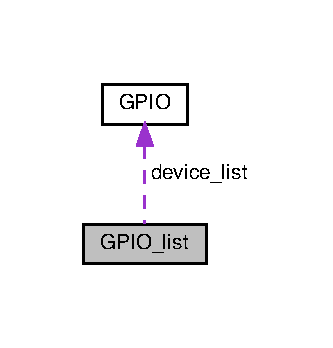
\includegraphics[width=160pt]{structGPIO__list__coll__graph}
\end{center}
\end{figure}
\subsection*{Data Fields}


\subsection{Detailed Description}
Struttura dati per la gestione di più device \hyperlink{structGPIO}{G\+P\+IO} da parte del driver. 

\subsection{Field Documentation}
\mbox{\Hypertarget{structGPIO__list_a170d1d78f27f6ab4c8badaaa4b3f2305}\label{structGPIO__list_a170d1d78f27f6ab4c8badaaa4b3f2305}} 
\index{G\+P\+I\+O\+\_\+list@{G\+P\+I\+O\+\_\+list}!device\+\_\+count@{device\+\_\+count}}
\index{device\+\_\+count@{device\+\_\+count}!G\+P\+I\+O\+\_\+list@{G\+P\+I\+O\+\_\+list}}
\subsubsection{\texorpdfstring{device\+\_\+count}{device\_count}}
{\footnotesize\ttfamily uint32\+\_\+t device\+\_\+count}

numero di device attivi e gestiti dal driver \mbox{\Hypertarget{structGPIO__list_a1f17219814029f429cd2f3fdf4190e0b}\label{structGPIO__list_a1f17219814029f429cd2f3fdf4190e0b}} 
\index{G\+P\+I\+O\+\_\+list@{G\+P\+I\+O\+\_\+list}!device\+\_\+list@{device\+\_\+list}}
\index{device\+\_\+list@{device\+\_\+list}!G\+P\+I\+O\+\_\+list@{G\+P\+I\+O\+\_\+list}}
\subsubsection{\texorpdfstring{device\+\_\+list}{device\_list}}
{\footnotesize\ttfamily \hyperlink{structGPIO}{G\+P\+IO}$\ast$$\ast$ device\+\_\+list}

array di puntatori a \hyperlink{structGPIO}{G\+P\+IO}, ciascuno dei quali si riferisce ad un device \mbox{\Hypertarget{structGPIO__list_aeff61809685e5df1b38aec1d871a49bb}\label{structGPIO__list_aeff61809685e5df1b38aec1d871a49bb}} 
\index{G\+P\+I\+O\+\_\+list@{G\+P\+I\+O\+\_\+list}!list\+\_\+size@{list\+\_\+size}}
\index{list\+\_\+size@{list\+\_\+size}!G\+P\+I\+O\+\_\+list@{G\+P\+I\+O\+\_\+list}}
\subsubsection{\texorpdfstring{list\+\_\+size}{list\_size}}
{\footnotesize\ttfamily uint32\+\_\+t list\+\_\+size}

dimensione della lista, ovvero il numero massimo di device gestibili 

The documentation for this struct was generated from the following file\+:\begin{DoxyCompactItemize}
\item 
/media/saverio/\+O\+S/\+Users/\+Saverio/\+Desktop/\+S\+E/git/codici\+\_\+da\+\_\+mandare/\+F\+P\+G\+A/\+G\+P\+I\+O/\+Driver/\+Kernel\+\_\+\+Mode/\hyperlink{GPIO__list_8h}{G\+P\+I\+O\+\_\+list.\+h}\end{DoxyCompactItemize}

\hypertarget{classGPIO__v1__0}{}\section{G\+P\+I\+O\+\_\+v1\+\_\+0 Entity Reference}
\label{classGPIO__v1__0}\index{G\+P\+I\+O\+\_\+v1\+\_\+0@{G\+P\+I\+O\+\_\+v1\+\_\+0}}


Inheritance diagram for G\+P\+I\+O\+\_\+v1\+\_\+0\+:\nopagebreak
\begin{figure}[H]
\begin{center}
\leavevmode
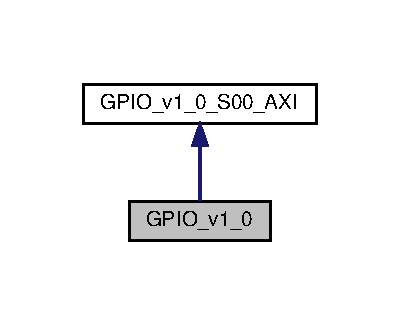
\includegraphics[width=192pt]{classGPIO__v1__0__inherit__graph}
\end{center}
\end{figure}


Collaboration diagram for G\+P\+I\+O\+\_\+v1\+\_\+0\+:\nopagebreak
\begin{figure}[H]
\begin{center}
\leavevmode
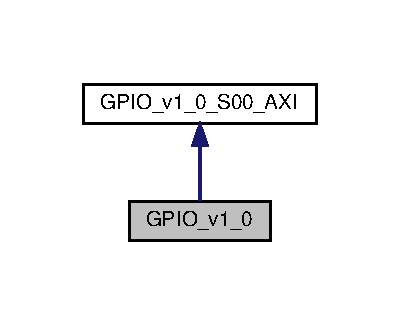
\includegraphics[width=192pt]{classGPIO__v1__0__coll__graph}
\end{center}
\end{figure}
\subsection*{Entities}
\begin{DoxyCompactItemize}
\item 
\hyperlink{classGPIO__v1__0_1_1arch__imp}{arch\+\_\+imp} architecture
\end{DoxyCompactItemize}
\subsection*{Libraries}
 \begin{DoxyCompactItemize}
\item 
\mbox{\Hypertarget{classGPIO__v1__0_a0a6af6eef40212dbaf130d57ce711256}\label{classGPIO__v1__0_a0a6af6eef40212dbaf130d57ce711256}} 
\hyperlink{classGPIO__v1__0_a0a6af6eef40212dbaf130d57ce711256}{ieee} 
\begin{DoxyCompactList}\small\item\em Viene utilizzata la libreria I\+E\+EE. \end{DoxyCompactList}\end{DoxyCompactItemize}
\subsection*{Use Clauses}
 \begin{DoxyCompactItemize}
\item 
\mbox{\Hypertarget{classGPIO__v1__0_acd03516902501cd1c7296a98e22c6fcb}\label{classGPIO__v1__0_acd03516902501cd1c7296a98e22c6fcb}} 
\hyperlink{classGPIO__v1__0_acd03516902501cd1c7296a98e22c6fcb}{std\+\_\+logic\+\_\+1164}   
\begin{DoxyCompactList}\small\item\em Sono utilizzati i segnali della standard logic. \end{DoxyCompactList}\item 
\mbox{\Hypertarget{classGPIO__v1__0_a2edc34402b573437d5f25fa90ba4013e}\label{classGPIO__v1__0_a2edc34402b573437d5f25fa90ba4013e}} 
\hyperlink{classGPIO__v1__0_a2edc34402b573437d5f25fa90ba4013e}{numeric\+\_\+std}   
\begin{DoxyCompactList}\small\item\em Vengono utilizzate le funzioni numeriche. \end{DoxyCompactList}\end{DoxyCompactItemize}
\subsection*{Generics}
 \begin{DoxyCompactItemize}
\item 
\mbox{\Hypertarget{classGPIO__v1__0_a16bbf9205afa677edb8a74dcd39ebb9f}\label{classGPIO__v1__0_a16bbf9205afa677edb8a74dcd39ebb9f}} 
\hyperlink{classGPIO__v1__0_a16bbf9205afa677edb8a74dcd39ebb9f}{width} {\bfseries {\bfseries \textcolor{vhdlchar}{integer}\textcolor{vhdlchar}{ }\textcolor{vhdlchar}{ }\textcolor{vhdlchar}{\+:}\textcolor{vhdlchar}{=}\textcolor{vhdlchar}{ }\textcolor{vhdlchar}{ } \textcolor{vhdldigit}{4} \textcolor{vhdlchar}{ }}}
\begin{DoxyCompactList}\small\item\em determina il numero di \hyperlink{structGPIO}{G\+P\+IO} da controllare \end{DoxyCompactList}\item 
\mbox{\Hypertarget{classGPIO__v1__0_afce7943994a4ddfa81f224225976a4c7}\label{classGPIO__v1__0_afce7943994a4ddfa81f224225976a4c7}} 
\hyperlink{classGPIO__v1__0_afce7943994a4ddfa81f224225976a4c7}{C\+\_\+\+S00\+\_\+\+A\+X\+I\+\_\+\+D\+A\+T\+A\+\_\+\+W\+I\+D\+TH} {\bfseries {\bfseries \textcolor{vhdlchar}{integer}\textcolor{vhdlchar}{ }\textcolor{vhdlchar}{ }\textcolor{vhdlchar}{\+:}\textcolor{vhdlchar}{=}\textcolor{vhdlchar}{ }\textcolor{vhdlchar}{ } \textcolor{vhdldigit}{32} \textcolor{vhdlchar}{ }}}
\item 
\mbox{\Hypertarget{classGPIO__v1__0_ab7787f274c76bb896ac98fdcfb570c65}\label{classGPIO__v1__0_ab7787f274c76bb896ac98fdcfb570c65}} 
\hyperlink{classGPIO__v1__0_ab7787f274c76bb896ac98fdcfb570c65}{C\+\_\+\+S00\+\_\+\+A\+X\+I\+\_\+\+A\+D\+D\+R\+\_\+\+W\+I\+D\+TH} {\bfseries {\bfseries \textcolor{vhdlchar}{integer}\textcolor{vhdlchar}{ }\textcolor{vhdlchar}{ }\textcolor{vhdlchar}{\+:}\textcolor{vhdlchar}{=}\textcolor{vhdlchar}{ }\textcolor{vhdlchar}{ } \textcolor{vhdldigit}{5} \textcolor{vhdlchar}{ }}}
\end{DoxyCompactItemize}
\subsection*{Ports}
 \begin{DoxyCompactItemize}
\item 
\mbox{\Hypertarget{classGPIO__v1__0_ac0744a550c27f11ab186fd7a1156a54e}\label{classGPIO__v1__0_ac0744a550c27f11ab186fd7a1156a54e}} 
\hyperlink{classGPIO__v1__0_ac0744a550c27f11ab186fd7a1156a54e}{pads}  {\bfseries {\bfseries \textcolor{vhdlchar}{inout}\textcolor{vhdlchar}{ }}} {\bfseries \textcolor{vhdlchar}{std\+\_\+logic\+\_\+vector}\textcolor{vhdlchar}{ }\textcolor{vhdlchar}{(}\textcolor{vhdlchar}{ }\textcolor{vhdlchar}{ }\textcolor{vhdlchar}{ }\textcolor{vhdlchar}{ }{\bfseries \hyperlink{classGPIO__v1__0_a16bbf9205afa677edb8a74dcd39ebb9f}{width}} \textcolor{vhdlchar}{-\/}\textcolor{vhdlchar}{ } \textcolor{vhdldigit}{1} \textcolor{vhdlchar}{ }\textcolor{vhdlchar}{downto}\textcolor{vhdlchar}{ }\textcolor{vhdlchar}{ } \textcolor{vhdldigit}{0} \textcolor{vhdlchar}{ }\textcolor{vhdlchar}{)}\textcolor{vhdlchar}{ }} 
\begin{DoxyCompactList}\small\item\em se \hyperlink{structGPIO}{G\+P\+IO} in modalità lettura mostra il valore letto, altrimenti forza un valore in uscita \end{DoxyCompactList}\item 
\mbox{\Hypertarget{classGPIO__v1__0_a5b78f3e3edfaf6e8ec79031b9e631e9d}\label{classGPIO__v1__0_a5b78f3e3edfaf6e8ec79031b9e631e9d}} 
\hyperlink{classGPIO__v1__0_a5b78f3e3edfaf6e8ec79031b9e631e9d}{interrupt}  {\bfseries {\bfseries \textcolor{vhdlchar}{out}\textcolor{vhdlchar}{ }}} {\bfseries \textcolor{vhdlchar}{std\+\_\+logic}\textcolor{vhdlchar}{ }} 
\begin{DoxyCompactList}\small\item\em segnale di interrupt \end{DoxyCompactList}\item 
\mbox{\Hypertarget{classGPIO__v1__0_a037f9e3df8559bfd59db37bcba9cb7a8}\label{classGPIO__v1__0_a037f9e3df8559bfd59db37bcba9cb7a8}} 
\hyperlink{classGPIO__v1__0_a037f9e3df8559bfd59db37bcba9cb7a8}{s00\+\_\+axi\+\_\+aclk}  {\bfseries {\bfseries \textcolor{vhdlchar}{in}\textcolor{vhdlchar}{ }}} {\bfseries \textcolor{vhdlchar}{std\+\_\+logic}\textcolor{vhdlchar}{ }} 
\item 
\mbox{\Hypertarget{classGPIO__v1__0_a8249c106fbd80196dcad2666c9f0b3fc}\label{classGPIO__v1__0_a8249c106fbd80196dcad2666c9f0b3fc}} 
\hyperlink{classGPIO__v1__0_a8249c106fbd80196dcad2666c9f0b3fc}{s00\+\_\+axi\+\_\+aresetn}  {\bfseries {\bfseries \textcolor{vhdlchar}{in}\textcolor{vhdlchar}{ }}} {\bfseries \textcolor{vhdlchar}{std\+\_\+logic}\textcolor{vhdlchar}{ }} 
\item 
\mbox{\Hypertarget{classGPIO__v1__0_a9fe80d3cc7f862afb670536e4e05dbeb}\label{classGPIO__v1__0_a9fe80d3cc7f862afb670536e4e05dbeb}} 
\hyperlink{classGPIO__v1__0_a9fe80d3cc7f862afb670536e4e05dbeb}{s00\+\_\+axi\+\_\+awaddr}  {\bfseries {\bfseries \textcolor{vhdlchar}{in}\textcolor{vhdlchar}{ }}} {\bfseries \textcolor{vhdlchar}{std\+\_\+logic\+\_\+vector}\textcolor{vhdlchar}{ }\textcolor{vhdlchar}{(}\textcolor{vhdlchar}{ }\textcolor{vhdlchar}{ }\textcolor{vhdlchar}{ }\textcolor{vhdlchar}{ }\textcolor{vhdlchar}{C\+\_\+\+S00\+\_\+\+A\+X\+I\+\_\+\+A\+D\+D\+R\+\_\+\+W\+I\+D\+TH}\textcolor{vhdlchar}{-\/}\textcolor{vhdlchar}{ } \textcolor{vhdldigit}{1} \textcolor{vhdlchar}{ }\textcolor{vhdlchar}{downto}\textcolor{vhdlchar}{ }\textcolor{vhdlchar}{ } \textcolor{vhdldigit}{0} \textcolor{vhdlchar}{ }\textcolor{vhdlchar}{)}\textcolor{vhdlchar}{ }} 
\item 
\mbox{\Hypertarget{classGPIO__v1__0_a719659c1addef5432978cc949d9e10ed}\label{classGPIO__v1__0_a719659c1addef5432978cc949d9e10ed}} 
\hyperlink{classGPIO__v1__0_a719659c1addef5432978cc949d9e10ed}{s00\+\_\+axi\+\_\+awprot}  {\bfseries {\bfseries \textcolor{vhdlchar}{in}\textcolor{vhdlchar}{ }}} {\bfseries \textcolor{vhdlchar}{std\+\_\+logic\+\_\+vector}\textcolor{vhdlchar}{ }\textcolor{vhdlchar}{(}\textcolor{vhdlchar}{ }\textcolor{vhdlchar}{ } \textcolor{vhdldigit}{2} \textcolor{vhdlchar}{ }\textcolor{vhdlchar}{downto}\textcolor{vhdlchar}{ }\textcolor{vhdlchar}{ } \textcolor{vhdldigit}{0} \textcolor{vhdlchar}{ }\textcolor{vhdlchar}{)}\textcolor{vhdlchar}{ }} 
\item 
\mbox{\Hypertarget{classGPIO__v1__0_a45aa02a72ae1a8389346d47173c60ed0}\label{classGPIO__v1__0_a45aa02a72ae1a8389346d47173c60ed0}} 
\hyperlink{classGPIO__v1__0_a45aa02a72ae1a8389346d47173c60ed0}{s00\+\_\+axi\+\_\+awvalid}  {\bfseries {\bfseries \textcolor{vhdlchar}{in}\textcolor{vhdlchar}{ }}} {\bfseries \textcolor{vhdlchar}{std\+\_\+logic}\textcolor{vhdlchar}{ }} 
\item 
\mbox{\Hypertarget{classGPIO__v1__0_ad0a1f71502d91a45dbc6c365f85c6566}\label{classGPIO__v1__0_ad0a1f71502d91a45dbc6c365f85c6566}} 
\hyperlink{classGPIO__v1__0_ad0a1f71502d91a45dbc6c365f85c6566}{s00\+\_\+axi\+\_\+awready}  {\bfseries {\bfseries \textcolor{vhdlchar}{out}\textcolor{vhdlchar}{ }}} {\bfseries \textcolor{vhdlchar}{std\+\_\+logic}\textcolor{vhdlchar}{ }} 
\item 
\mbox{\Hypertarget{classGPIO__v1__0_ae2b15b55ee463fd9dd030ee29db6bb17}\label{classGPIO__v1__0_ae2b15b55ee463fd9dd030ee29db6bb17}} 
\hyperlink{classGPIO__v1__0_ae2b15b55ee463fd9dd030ee29db6bb17}{s00\+\_\+axi\+\_\+wdata}  {\bfseries {\bfseries \textcolor{vhdlchar}{in}\textcolor{vhdlchar}{ }}} {\bfseries \textcolor{vhdlchar}{std\+\_\+logic\+\_\+vector}\textcolor{vhdlchar}{ }\textcolor{vhdlchar}{(}\textcolor{vhdlchar}{ }\textcolor{vhdlchar}{ }\textcolor{vhdlchar}{ }\textcolor{vhdlchar}{ }\textcolor{vhdlchar}{C\+\_\+\+S00\+\_\+\+A\+X\+I\+\_\+\+D\+A\+T\+A\+\_\+\+W\+I\+D\+TH}\textcolor{vhdlchar}{-\/}\textcolor{vhdlchar}{ } \textcolor{vhdldigit}{1} \textcolor{vhdlchar}{ }\textcolor{vhdlchar}{downto}\textcolor{vhdlchar}{ }\textcolor{vhdlchar}{ } \textcolor{vhdldigit}{0} \textcolor{vhdlchar}{ }\textcolor{vhdlchar}{)}\textcolor{vhdlchar}{ }} 
\item 
\mbox{\Hypertarget{classGPIO__v1__0_a120924bc3fd5fd10ec0f96e19c3f4904}\label{classGPIO__v1__0_a120924bc3fd5fd10ec0f96e19c3f4904}} 
\hyperlink{classGPIO__v1__0_a120924bc3fd5fd10ec0f96e19c3f4904}{s00\+\_\+axi\+\_\+wstrb}  {\bfseries {\bfseries \textcolor{vhdlchar}{in}\textcolor{vhdlchar}{ }}} {\bfseries \textcolor{vhdlchar}{std\+\_\+logic\+\_\+vector}\textcolor{vhdlchar}{ }\textcolor{vhdlchar}{(}\textcolor{vhdlchar}{ }\textcolor{vhdlchar}{(}\textcolor{vhdlchar}{ }\textcolor{vhdlchar}{ }\textcolor{vhdlchar}{ }\textcolor{vhdlchar}{ }\textcolor{vhdlchar}{C\+\_\+\+S00\+\_\+\+A\+X\+I\+\_\+\+D\+A\+T\+A\+\_\+\+W\+I\+D\+TH}\textcolor{vhdlchar}{/}\textcolor{vhdlchar}{ } \textcolor{vhdldigit}{8} \textcolor{vhdlchar}{ }\textcolor{vhdlchar}{)}\textcolor{vhdlchar}{ }\textcolor{vhdlchar}{-\/}\textcolor{vhdlchar}{ } \textcolor{vhdldigit}{1} \textcolor{vhdlchar}{ }\textcolor{vhdlchar}{downto}\textcolor{vhdlchar}{ }\textcolor{vhdlchar}{ } \textcolor{vhdldigit}{0} \textcolor{vhdlchar}{ }\textcolor{vhdlchar}{)}\textcolor{vhdlchar}{ }} 
\item 
\mbox{\Hypertarget{classGPIO__v1__0_a24e90907193647007d2947353740114d}\label{classGPIO__v1__0_a24e90907193647007d2947353740114d}} 
\hyperlink{classGPIO__v1__0_a24e90907193647007d2947353740114d}{s00\+\_\+axi\+\_\+wvalid}  {\bfseries {\bfseries \textcolor{vhdlchar}{in}\textcolor{vhdlchar}{ }}} {\bfseries \textcolor{vhdlchar}{std\+\_\+logic}\textcolor{vhdlchar}{ }} 
\item 
\mbox{\Hypertarget{classGPIO__v1__0_a3fc60abc0cfbfa90003a83bffdd476c4}\label{classGPIO__v1__0_a3fc60abc0cfbfa90003a83bffdd476c4}} 
\hyperlink{classGPIO__v1__0_a3fc60abc0cfbfa90003a83bffdd476c4}{s00\+\_\+axi\+\_\+wready}  {\bfseries {\bfseries \textcolor{vhdlchar}{out}\textcolor{vhdlchar}{ }}} {\bfseries \textcolor{vhdlchar}{std\+\_\+logic}\textcolor{vhdlchar}{ }} 
\item 
\mbox{\Hypertarget{classGPIO__v1__0_af8799be946d3f5354263e7deb15f94f1}\label{classGPIO__v1__0_af8799be946d3f5354263e7deb15f94f1}} 
\hyperlink{classGPIO__v1__0_af8799be946d3f5354263e7deb15f94f1}{s00\+\_\+axi\+\_\+bresp}  {\bfseries {\bfseries \textcolor{vhdlchar}{out}\textcolor{vhdlchar}{ }}} {\bfseries \textcolor{vhdlchar}{std\+\_\+logic\+\_\+vector}\textcolor{vhdlchar}{ }\textcolor{vhdlchar}{(}\textcolor{vhdlchar}{ }\textcolor{vhdlchar}{ } \textcolor{vhdldigit}{1} \textcolor{vhdlchar}{ }\textcolor{vhdlchar}{downto}\textcolor{vhdlchar}{ }\textcolor{vhdlchar}{ } \textcolor{vhdldigit}{0} \textcolor{vhdlchar}{ }\textcolor{vhdlchar}{)}\textcolor{vhdlchar}{ }} 
\item 
\mbox{\Hypertarget{classGPIO__v1__0_a5110b7dd4fb9548a2aab88f50dbe1d5e}\label{classGPIO__v1__0_a5110b7dd4fb9548a2aab88f50dbe1d5e}} 
\hyperlink{classGPIO__v1__0_a5110b7dd4fb9548a2aab88f50dbe1d5e}{s00\+\_\+axi\+\_\+bvalid}  {\bfseries {\bfseries \textcolor{vhdlchar}{out}\textcolor{vhdlchar}{ }}} {\bfseries \textcolor{vhdlchar}{std\+\_\+logic}\textcolor{vhdlchar}{ }} 
\item 
\mbox{\Hypertarget{classGPIO__v1__0_a1ef2019b0613bc23d4829eeeb24eb98d}\label{classGPIO__v1__0_a1ef2019b0613bc23d4829eeeb24eb98d}} 
\hyperlink{classGPIO__v1__0_a1ef2019b0613bc23d4829eeeb24eb98d}{s00\+\_\+axi\+\_\+bready}  {\bfseries {\bfseries \textcolor{vhdlchar}{in}\textcolor{vhdlchar}{ }}} {\bfseries \textcolor{vhdlchar}{std\+\_\+logic}\textcolor{vhdlchar}{ }} 
\item 
\mbox{\Hypertarget{classGPIO__v1__0_af70a86336cd6505064e45b69f4623939}\label{classGPIO__v1__0_af70a86336cd6505064e45b69f4623939}} 
\hyperlink{classGPIO__v1__0_af70a86336cd6505064e45b69f4623939}{s00\+\_\+axi\+\_\+araddr}  {\bfseries {\bfseries \textcolor{vhdlchar}{in}\textcolor{vhdlchar}{ }}} {\bfseries \textcolor{vhdlchar}{std\+\_\+logic\+\_\+vector}\textcolor{vhdlchar}{ }\textcolor{vhdlchar}{(}\textcolor{vhdlchar}{ }\textcolor{vhdlchar}{ }\textcolor{vhdlchar}{ }\textcolor{vhdlchar}{ }\textcolor{vhdlchar}{C\+\_\+\+S00\+\_\+\+A\+X\+I\+\_\+\+A\+D\+D\+R\+\_\+\+W\+I\+D\+TH}\textcolor{vhdlchar}{-\/}\textcolor{vhdlchar}{ } \textcolor{vhdldigit}{1} \textcolor{vhdlchar}{ }\textcolor{vhdlchar}{downto}\textcolor{vhdlchar}{ }\textcolor{vhdlchar}{ } \textcolor{vhdldigit}{0} \textcolor{vhdlchar}{ }\textcolor{vhdlchar}{)}\textcolor{vhdlchar}{ }} 
\item 
\mbox{\Hypertarget{classGPIO__v1__0_adc648df07895bf808b8c721e1dc6811b}\label{classGPIO__v1__0_adc648df07895bf808b8c721e1dc6811b}} 
\hyperlink{classGPIO__v1__0_adc648df07895bf808b8c721e1dc6811b}{s00\+\_\+axi\+\_\+arprot}  {\bfseries {\bfseries \textcolor{vhdlchar}{in}\textcolor{vhdlchar}{ }}} {\bfseries \textcolor{vhdlchar}{std\+\_\+logic\+\_\+vector}\textcolor{vhdlchar}{ }\textcolor{vhdlchar}{(}\textcolor{vhdlchar}{ }\textcolor{vhdlchar}{ } \textcolor{vhdldigit}{2} \textcolor{vhdlchar}{ }\textcolor{vhdlchar}{downto}\textcolor{vhdlchar}{ }\textcolor{vhdlchar}{ } \textcolor{vhdldigit}{0} \textcolor{vhdlchar}{ }\textcolor{vhdlchar}{)}\textcolor{vhdlchar}{ }} 
\item 
\mbox{\Hypertarget{classGPIO__v1__0_a94b78b2ae3cd13860f15afbdfb199e44}\label{classGPIO__v1__0_a94b78b2ae3cd13860f15afbdfb199e44}} 
\hyperlink{classGPIO__v1__0_a94b78b2ae3cd13860f15afbdfb199e44}{s00\+\_\+axi\+\_\+arvalid}  {\bfseries {\bfseries \textcolor{vhdlchar}{in}\textcolor{vhdlchar}{ }}} {\bfseries \textcolor{vhdlchar}{std\+\_\+logic}\textcolor{vhdlchar}{ }} 
\item 
\mbox{\Hypertarget{classGPIO__v1__0_ad35bd95f3352ff8dbdaea55205a98e53}\label{classGPIO__v1__0_ad35bd95f3352ff8dbdaea55205a98e53}} 
\hyperlink{classGPIO__v1__0_ad35bd95f3352ff8dbdaea55205a98e53}{s00\+\_\+axi\+\_\+arready}  {\bfseries {\bfseries \textcolor{vhdlchar}{out}\textcolor{vhdlchar}{ }}} {\bfseries \textcolor{vhdlchar}{std\+\_\+logic}\textcolor{vhdlchar}{ }} 
\item 
\mbox{\Hypertarget{classGPIO__v1__0_ad2655fadb987e0487c428aca187b55d0}\label{classGPIO__v1__0_ad2655fadb987e0487c428aca187b55d0}} 
\hyperlink{classGPIO__v1__0_ad2655fadb987e0487c428aca187b55d0}{s00\+\_\+axi\+\_\+rdata}  {\bfseries {\bfseries \textcolor{vhdlchar}{out}\textcolor{vhdlchar}{ }}} {\bfseries \textcolor{vhdlchar}{std\+\_\+logic\+\_\+vector}\textcolor{vhdlchar}{ }\textcolor{vhdlchar}{(}\textcolor{vhdlchar}{ }\textcolor{vhdlchar}{ }\textcolor{vhdlchar}{ }\textcolor{vhdlchar}{ }\textcolor{vhdlchar}{C\+\_\+\+S00\+\_\+\+A\+X\+I\+\_\+\+D\+A\+T\+A\+\_\+\+W\+I\+D\+TH}\textcolor{vhdlchar}{-\/}\textcolor{vhdlchar}{ } \textcolor{vhdldigit}{1} \textcolor{vhdlchar}{ }\textcolor{vhdlchar}{downto}\textcolor{vhdlchar}{ }\textcolor{vhdlchar}{ } \textcolor{vhdldigit}{0} \textcolor{vhdlchar}{ }\textcolor{vhdlchar}{)}\textcolor{vhdlchar}{ }} 
\item 
\mbox{\Hypertarget{classGPIO__v1__0_a1acee955f50f71e5595a03c6ca301cf0}\label{classGPIO__v1__0_a1acee955f50f71e5595a03c6ca301cf0}} 
\hyperlink{classGPIO__v1__0_a1acee955f50f71e5595a03c6ca301cf0}{s00\+\_\+axi\+\_\+rresp}  {\bfseries {\bfseries \textcolor{vhdlchar}{out}\textcolor{vhdlchar}{ }}} {\bfseries \textcolor{vhdlchar}{std\+\_\+logic\+\_\+vector}\textcolor{vhdlchar}{ }\textcolor{vhdlchar}{(}\textcolor{vhdlchar}{ }\textcolor{vhdlchar}{ } \textcolor{vhdldigit}{1} \textcolor{vhdlchar}{ }\textcolor{vhdlchar}{downto}\textcolor{vhdlchar}{ }\textcolor{vhdlchar}{ } \textcolor{vhdldigit}{0} \textcolor{vhdlchar}{ }\textcolor{vhdlchar}{)}\textcolor{vhdlchar}{ }} 
\item 
\mbox{\Hypertarget{classGPIO__v1__0_af180911f7eb262e530e26865bc97aa0b}\label{classGPIO__v1__0_af180911f7eb262e530e26865bc97aa0b}} 
\hyperlink{classGPIO__v1__0_af180911f7eb262e530e26865bc97aa0b}{s00\+\_\+axi\+\_\+rvalid}  {\bfseries {\bfseries \textcolor{vhdlchar}{out}\textcolor{vhdlchar}{ }}} {\bfseries \textcolor{vhdlchar}{std\+\_\+logic}\textcolor{vhdlchar}{ }} 
\item 
\mbox{\Hypertarget{classGPIO__v1__0_a8b82eb165d7024f6c7b25646f6ebdd4d}\label{classGPIO__v1__0_a8b82eb165d7024f6c7b25646f6ebdd4d}} 
\hyperlink{classGPIO__v1__0_a8b82eb165d7024f6c7b25646f6ebdd4d}{s00\+\_\+axi\+\_\+rready}  {\bfseries {\bfseries \textcolor{vhdlchar}{in}\textcolor{vhdlchar}{ }}} {\bfseries \textcolor{vhdlchar}{std\+\_\+logic}\textcolor{vhdlchar}{ }} 
\end{DoxyCompactItemize}


The documentation for this class was generated from the following file\+:\begin{DoxyCompactItemize}
\item 
/media/saverio/\+O\+S/\+Users/\+Saverio/\+Desktop/\+S\+E/git/codici\+\_\+da\+\_\+mandare/\+F\+P\+G\+A/\+G\+P\+I\+O/\+Hardware/\+G\+P\+I\+O\+\_\+1.\+0/hdl/\hyperlink{GPIO__v1__0_8vhd}{G\+P\+I\+O\+\_\+v1\+\_\+0.\+vhd}\end{DoxyCompactItemize}

\hypertarget{classGPIO__v1__0__S00__AXI}{}\section{G\+P\+I\+O\+\_\+v1\+\_\+0\+\_\+\+S00\+\_\+\+A\+XI Entity Reference}
\label{classGPIO__v1__0__S00__AXI}\index{G\+P\+I\+O\+\_\+v1\+\_\+0\+\_\+\+S00\+\_\+\+A\+XI@{G\+P\+I\+O\+\_\+v1\+\_\+0\+\_\+\+S00\+\_\+\+A\+XI}}


Inheritance diagram for G\+P\+I\+O\+\_\+v1\+\_\+0\+\_\+\+S00\+\_\+\+A\+XI\+:\nopagebreak
\begin{figure}[H]
\begin{center}
\leavevmode
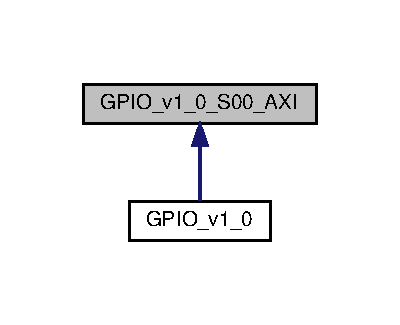
\includegraphics[width=192pt]{classGPIO__v1__0__S00__AXI__inherit__graph}
\end{center}
\end{figure}
\subsection*{Entities}
\begin{DoxyCompactItemize}
\item 
\hyperlink{classGPIO__v1__0__S00__AXI_1_1arch__imp}{arch\+\_\+imp} architecture
\end{DoxyCompactItemize}
\subsection*{Libraries}
 \begin{DoxyCompactItemize}
\item 
\mbox{\Hypertarget{classGPIO__v1__0__S00__AXI_a0a6af6eef40212dbaf130d57ce711256}\label{classGPIO__v1__0__S00__AXI_a0a6af6eef40212dbaf130d57ce711256}} 
\hyperlink{classGPIO__v1__0__S00__AXI_a0a6af6eef40212dbaf130d57ce711256}{ieee} 
\begin{DoxyCompactList}\small\item\em Viene utilizzato la libreria I\+E\+EE. \end{DoxyCompactList}\end{DoxyCompactItemize}
\subsection*{Use Clauses}
 \begin{DoxyCompactItemize}
\item 
\mbox{\Hypertarget{classGPIO__v1__0__S00__AXI_acd03516902501cd1c7296a98e22c6fcb}\label{classGPIO__v1__0__S00__AXI_acd03516902501cd1c7296a98e22c6fcb}} 
\hyperlink{classGPIO__v1__0__S00__AXI_acd03516902501cd1c7296a98e22c6fcb}{std\+\_\+logic\+\_\+1164}   
\begin{DoxyCompactList}\small\item\em Sono utilizzati i segnali della standard logic. \end{DoxyCompactList}\item 
\mbox{\Hypertarget{classGPIO__v1__0__S00__AXI_a2edc34402b573437d5f25fa90ba4013e}\label{classGPIO__v1__0__S00__AXI_a2edc34402b573437d5f25fa90ba4013e}} 
\hyperlink{classGPIO__v1__0__S00__AXI_a2edc34402b573437d5f25fa90ba4013e}{numeric\+\_\+std}   
\begin{DoxyCompactList}\small\item\em Vengono utilizzate le funzioni numeriche. \end{DoxyCompactList}\item 
\mbox{\Hypertarget{classGPIO__v1__0__S00__AXI_acb2d98d781f19c8f5f4109576ec45502}\label{classGPIO__v1__0__S00__AXI_acb2d98d781f19c8f5f4109576ec45502}} 
\hyperlink{classGPIO__v1__0__S00__AXI_acb2d98d781f19c8f5f4109576ec45502}{std\+\_\+logic\+\_\+misc}   
\begin{DoxyCompactList}\small\item\em Viene utilizzata la libreria misc di utility. \end{DoxyCompactList}\end{DoxyCompactItemize}
\subsection*{Generics}
 \begin{DoxyCompactItemize}
\item 
\mbox{\Hypertarget{classGPIO__v1__0__S00__AXI_a16bbf9205afa677edb8a74dcd39ebb9f}\label{classGPIO__v1__0__S00__AXI_a16bbf9205afa677edb8a74dcd39ebb9f}} 
\hyperlink{classGPIO__v1__0__S00__AXI_a16bbf9205afa677edb8a74dcd39ebb9f}{width} {\bfseries {\bfseries \textcolor{vhdlchar}{integer}\textcolor{vhdlchar}{ }\textcolor{vhdlchar}{ }\textcolor{vhdlchar}{\+:}\textcolor{vhdlchar}{=}\textcolor{vhdlchar}{ }\textcolor{vhdlchar}{ } \textcolor{vhdldigit}{4} \textcolor{vhdlchar}{ }}}
\begin{DoxyCompactList}\small\item\em determina il numero di \hyperlink{structGPIO}{G\+P\+IO} da controllare \end{DoxyCompactList}\item 
\mbox{\Hypertarget{classGPIO__v1__0__S00__AXI_a0fad312acd1f302ce7de30c5658df0bd}\label{classGPIO__v1__0__S00__AXI_a0fad312acd1f302ce7de30c5658df0bd}} 
\hyperlink{classGPIO__v1__0__S00__AXI_a0fad312acd1f302ce7de30c5658df0bd}{C\+\_\+\+S\+\_\+\+A\+X\+I\+\_\+\+D\+A\+T\+A\+\_\+\+W\+I\+D\+TH} {\bfseries {\bfseries \textcolor{vhdlchar}{integer}\textcolor{vhdlchar}{ }\textcolor{vhdlchar}{ }\textcolor{vhdlchar}{\+:}\textcolor{vhdlchar}{=}\textcolor{vhdlchar}{ }\textcolor{vhdlchar}{ } \textcolor{vhdldigit}{32} \textcolor{vhdlchar}{ }}}
\item 
\mbox{\Hypertarget{classGPIO__v1__0__S00__AXI_a9abff2eaa069440f3b7d9e9937d5ee8e}\label{classGPIO__v1__0__S00__AXI_a9abff2eaa069440f3b7d9e9937d5ee8e}} 
\hyperlink{classGPIO__v1__0__S00__AXI_a9abff2eaa069440f3b7d9e9937d5ee8e}{C\+\_\+\+S\+\_\+\+A\+X\+I\+\_\+\+A\+D\+D\+R\+\_\+\+W\+I\+D\+TH} {\bfseries {\bfseries \textcolor{vhdlchar}{integer}\textcolor{vhdlchar}{ }\textcolor{vhdlchar}{ }\textcolor{vhdlchar}{\+:}\textcolor{vhdlchar}{=}\textcolor{vhdlchar}{ }\textcolor{vhdlchar}{ } \textcolor{vhdldigit}{5} \textcolor{vhdlchar}{ }}}
\end{DoxyCompactItemize}
\subsection*{Ports}
 \begin{DoxyCompactItemize}
\item 
\mbox{\Hypertarget{classGPIO__v1__0__S00__AXI_ac0744a550c27f11ab186fd7a1156a54e}\label{classGPIO__v1__0__S00__AXI_ac0744a550c27f11ab186fd7a1156a54e}} 
\hyperlink{classGPIO__v1__0__S00__AXI_ac0744a550c27f11ab186fd7a1156a54e}{pads}  {\bfseries {\bfseries \textcolor{vhdlchar}{inout}\textcolor{vhdlchar}{ }}} {\bfseries \textcolor{vhdlchar}{std\+\_\+logic\+\_\+vector}\textcolor{vhdlchar}{ }\textcolor{vhdlchar}{(}\textcolor{vhdlchar}{ }\textcolor{vhdlchar}{ }\textcolor{vhdlchar}{ }\textcolor{vhdlchar}{ }{\bfseries \hyperlink{classGPIO__v1__0__S00__AXI_a16bbf9205afa677edb8a74dcd39ebb9f}{width}} \textcolor{vhdlchar}{-\/}\textcolor{vhdlchar}{ } \textcolor{vhdldigit}{1} \textcolor{vhdlchar}{ }\textcolor{vhdlchar}{downto}\textcolor{vhdlchar}{ }\textcolor{vhdlchar}{ } \textcolor{vhdldigit}{0} \textcolor{vhdlchar}{ }\textcolor{vhdlchar}{)}\textcolor{vhdlchar}{ }} 
\begin{DoxyCompactList}\small\item\em se \hyperlink{structGPIO}{G\+P\+IO} in modalità lettura mostra il valore letto, altrimenti forza un valore in uscita \end{DoxyCompactList}\item 
\mbox{\Hypertarget{classGPIO__v1__0__S00__AXI_a5b78f3e3edfaf6e8ec79031b9e631e9d}\label{classGPIO__v1__0__S00__AXI_a5b78f3e3edfaf6e8ec79031b9e631e9d}} 
\hyperlink{classGPIO__v1__0__S00__AXI_a5b78f3e3edfaf6e8ec79031b9e631e9d}{interrupt}  {\bfseries {\bfseries \textcolor{vhdlchar}{out}\textcolor{vhdlchar}{ }}} {\bfseries \textcolor{vhdlchar}{std\+\_\+logic}\textcolor{vhdlchar}{ }} 
\begin{DoxyCompactList}\small\item\em segnale di interrupt \end{DoxyCompactList}\item 
\mbox{\Hypertarget{classGPIO__v1__0__S00__AXI_a3f54d782a88290bdaa6baffd7cd84ab4}\label{classGPIO__v1__0__S00__AXI_a3f54d782a88290bdaa6baffd7cd84ab4}} 
\hyperlink{classGPIO__v1__0__S00__AXI_a3f54d782a88290bdaa6baffd7cd84ab4}{S\+\_\+\+A\+X\+I\+\_\+\+A\+C\+LK}  {\bfseries {\bfseries \textcolor{vhdlchar}{in}\textcolor{vhdlchar}{ }}} {\bfseries \textcolor{vhdlchar}{std\+\_\+logic}\textcolor{vhdlchar}{ }} 
\item 
\mbox{\Hypertarget{classGPIO__v1__0__S00__AXI_a089b396e17dee353ccc7d5389dda5532}\label{classGPIO__v1__0__S00__AXI_a089b396e17dee353ccc7d5389dda5532}} 
\hyperlink{classGPIO__v1__0__S00__AXI_a089b396e17dee353ccc7d5389dda5532}{S\+\_\+\+A\+X\+I\+\_\+\+A\+R\+E\+S\+E\+TN}  {\bfseries {\bfseries \textcolor{vhdlchar}{in}\textcolor{vhdlchar}{ }}} {\bfseries \textcolor{vhdlchar}{std\+\_\+logic}\textcolor{vhdlchar}{ }} 
\item 
\mbox{\Hypertarget{classGPIO__v1__0__S00__AXI_a61cc7b190ba9d540e56941330e4a0883}\label{classGPIO__v1__0__S00__AXI_a61cc7b190ba9d540e56941330e4a0883}} 
\hyperlink{classGPIO__v1__0__S00__AXI_a61cc7b190ba9d540e56941330e4a0883}{S\+\_\+\+A\+X\+I\+\_\+\+A\+W\+A\+D\+DR}  {\bfseries {\bfseries \textcolor{vhdlchar}{in}\textcolor{vhdlchar}{ }}} {\bfseries \textcolor{vhdlchar}{std\+\_\+logic\+\_\+vector}\textcolor{vhdlchar}{ }\textcolor{vhdlchar}{(}\textcolor{vhdlchar}{ }\textcolor{vhdlchar}{ }\textcolor{vhdlchar}{ }\textcolor{vhdlchar}{ }\textcolor{vhdlchar}{C\+\_\+\+S\+\_\+\+A\+X\+I\+\_\+\+A\+D\+D\+R\+\_\+\+W\+I\+D\+TH}\textcolor{vhdlchar}{-\/}\textcolor{vhdlchar}{ } \textcolor{vhdldigit}{1} \textcolor{vhdlchar}{ }\textcolor{vhdlchar}{downto}\textcolor{vhdlchar}{ }\textcolor{vhdlchar}{ } \textcolor{vhdldigit}{0} \textcolor{vhdlchar}{ }\textcolor{vhdlchar}{)}\textcolor{vhdlchar}{ }} 
\item 
\mbox{\Hypertarget{classGPIO__v1__0__S00__AXI_a459abcd98567ad24261377eed899593a}\label{classGPIO__v1__0__S00__AXI_a459abcd98567ad24261377eed899593a}} 
\hyperlink{classGPIO__v1__0__S00__AXI_a459abcd98567ad24261377eed899593a}{S\+\_\+\+A\+X\+I\+\_\+\+A\+W\+P\+R\+OT}  {\bfseries {\bfseries \textcolor{vhdlchar}{in}\textcolor{vhdlchar}{ }}} {\bfseries \textcolor{vhdlchar}{std\+\_\+logic\+\_\+vector}\textcolor{vhdlchar}{ }\textcolor{vhdlchar}{(}\textcolor{vhdlchar}{ }\textcolor{vhdlchar}{ } \textcolor{vhdldigit}{2} \textcolor{vhdlchar}{ }\textcolor{vhdlchar}{downto}\textcolor{vhdlchar}{ }\textcolor{vhdlchar}{ } \textcolor{vhdldigit}{0} \textcolor{vhdlchar}{ }\textcolor{vhdlchar}{)}\textcolor{vhdlchar}{ }} 
\item 
\mbox{\Hypertarget{classGPIO__v1__0__S00__AXI_af1f1cbf67bf647ba58353c261719a3a0}\label{classGPIO__v1__0__S00__AXI_af1f1cbf67bf647ba58353c261719a3a0}} 
\hyperlink{classGPIO__v1__0__S00__AXI_af1f1cbf67bf647ba58353c261719a3a0}{S\+\_\+\+A\+X\+I\+\_\+\+A\+W\+V\+A\+L\+ID}  {\bfseries {\bfseries \textcolor{vhdlchar}{in}\textcolor{vhdlchar}{ }}} {\bfseries \textcolor{vhdlchar}{std\+\_\+logic}\textcolor{vhdlchar}{ }} 
\item 
\mbox{\Hypertarget{classGPIO__v1__0__S00__AXI_ac04aab5cc834e762e893e061016921c6}\label{classGPIO__v1__0__S00__AXI_ac04aab5cc834e762e893e061016921c6}} 
\hyperlink{classGPIO__v1__0__S00__AXI_ac04aab5cc834e762e893e061016921c6}{S\+\_\+\+A\+X\+I\+\_\+\+A\+W\+R\+E\+A\+DY}  {\bfseries {\bfseries \textcolor{vhdlchar}{out}\textcolor{vhdlchar}{ }}} {\bfseries \textcolor{vhdlchar}{std\+\_\+logic}\textcolor{vhdlchar}{ }} 
\item 
\mbox{\Hypertarget{classGPIO__v1__0__S00__AXI_a292e5db13719faf3a8b3aab091773467}\label{classGPIO__v1__0__S00__AXI_a292e5db13719faf3a8b3aab091773467}} 
\hyperlink{classGPIO__v1__0__S00__AXI_a292e5db13719faf3a8b3aab091773467}{S\+\_\+\+A\+X\+I\+\_\+\+W\+D\+A\+TA}  {\bfseries {\bfseries \textcolor{vhdlchar}{in}\textcolor{vhdlchar}{ }}} {\bfseries \textcolor{vhdlchar}{std\+\_\+logic\+\_\+vector}\textcolor{vhdlchar}{ }\textcolor{vhdlchar}{(}\textcolor{vhdlchar}{ }\textcolor{vhdlchar}{ }\textcolor{vhdlchar}{ }\textcolor{vhdlchar}{ }\textcolor{vhdlchar}{C\+\_\+\+S\+\_\+\+A\+X\+I\+\_\+\+D\+A\+T\+A\+\_\+\+W\+I\+D\+TH}\textcolor{vhdlchar}{-\/}\textcolor{vhdlchar}{ } \textcolor{vhdldigit}{1} \textcolor{vhdlchar}{ }\textcolor{vhdlchar}{downto}\textcolor{vhdlchar}{ }\textcolor{vhdlchar}{ } \textcolor{vhdldigit}{0} \textcolor{vhdlchar}{ }\textcolor{vhdlchar}{)}\textcolor{vhdlchar}{ }} 
\item 
\mbox{\Hypertarget{classGPIO__v1__0__S00__AXI_accd8e04b79540b57ab15fee1cb6c04f5}\label{classGPIO__v1__0__S00__AXI_accd8e04b79540b57ab15fee1cb6c04f5}} 
\hyperlink{classGPIO__v1__0__S00__AXI_accd8e04b79540b57ab15fee1cb6c04f5}{S\+\_\+\+A\+X\+I\+\_\+\+W\+S\+T\+RB}  {\bfseries {\bfseries \textcolor{vhdlchar}{in}\textcolor{vhdlchar}{ }}} {\bfseries \textcolor{vhdlchar}{std\+\_\+logic\+\_\+vector}\textcolor{vhdlchar}{ }\textcolor{vhdlchar}{(}\textcolor{vhdlchar}{ }\textcolor{vhdlchar}{(}\textcolor{vhdlchar}{ }\textcolor{vhdlchar}{ }\textcolor{vhdlchar}{ }\textcolor{vhdlchar}{ }\textcolor{vhdlchar}{C\+\_\+\+S\+\_\+\+A\+X\+I\+\_\+\+D\+A\+T\+A\+\_\+\+W\+I\+D\+TH}\textcolor{vhdlchar}{/}\textcolor{vhdlchar}{ } \textcolor{vhdldigit}{8} \textcolor{vhdlchar}{ }\textcolor{vhdlchar}{)}\textcolor{vhdlchar}{ }\textcolor{vhdlchar}{-\/}\textcolor{vhdlchar}{ } \textcolor{vhdldigit}{1} \textcolor{vhdlchar}{ }\textcolor{vhdlchar}{downto}\textcolor{vhdlchar}{ }\textcolor{vhdlchar}{ } \textcolor{vhdldigit}{0} \textcolor{vhdlchar}{ }\textcolor{vhdlchar}{)}\textcolor{vhdlchar}{ }} 
\item 
\mbox{\Hypertarget{classGPIO__v1__0__S00__AXI_a60bd882e2de781af9a7c6c3d494225d5}\label{classGPIO__v1__0__S00__AXI_a60bd882e2de781af9a7c6c3d494225d5}} 
\hyperlink{classGPIO__v1__0__S00__AXI_a60bd882e2de781af9a7c6c3d494225d5}{S\+\_\+\+A\+X\+I\+\_\+\+W\+V\+A\+L\+ID}  {\bfseries {\bfseries \textcolor{vhdlchar}{in}\textcolor{vhdlchar}{ }}} {\bfseries \textcolor{vhdlchar}{std\+\_\+logic}\textcolor{vhdlchar}{ }} 
\item 
\mbox{\Hypertarget{classGPIO__v1__0__S00__AXI_ab84e4db7037141a360c2b59f45124f01}\label{classGPIO__v1__0__S00__AXI_ab84e4db7037141a360c2b59f45124f01}} 
\hyperlink{classGPIO__v1__0__S00__AXI_ab84e4db7037141a360c2b59f45124f01}{S\+\_\+\+A\+X\+I\+\_\+\+W\+R\+E\+A\+DY}  {\bfseries {\bfseries \textcolor{vhdlchar}{out}\textcolor{vhdlchar}{ }}} {\bfseries \textcolor{vhdlchar}{std\+\_\+logic}\textcolor{vhdlchar}{ }} 
\item 
\mbox{\Hypertarget{classGPIO__v1__0__S00__AXI_abca6c9777b38a5a6bc04886924bafcc8}\label{classGPIO__v1__0__S00__AXI_abca6c9777b38a5a6bc04886924bafcc8}} 
\hyperlink{classGPIO__v1__0__S00__AXI_abca6c9777b38a5a6bc04886924bafcc8}{S\+\_\+\+A\+X\+I\+\_\+\+B\+R\+E\+SP}  {\bfseries {\bfseries \textcolor{vhdlchar}{out}\textcolor{vhdlchar}{ }}} {\bfseries \textcolor{vhdlchar}{std\+\_\+logic\+\_\+vector}\textcolor{vhdlchar}{ }\textcolor{vhdlchar}{(}\textcolor{vhdlchar}{ }\textcolor{vhdlchar}{ } \textcolor{vhdldigit}{1} \textcolor{vhdlchar}{ }\textcolor{vhdlchar}{downto}\textcolor{vhdlchar}{ }\textcolor{vhdlchar}{ } \textcolor{vhdldigit}{0} \textcolor{vhdlchar}{ }\textcolor{vhdlchar}{)}\textcolor{vhdlchar}{ }} 
\item 
\mbox{\Hypertarget{classGPIO__v1__0__S00__AXI_a58f260d3ebaa69be91bb65ff9211823b}\label{classGPIO__v1__0__S00__AXI_a58f260d3ebaa69be91bb65ff9211823b}} 
\hyperlink{classGPIO__v1__0__S00__AXI_a58f260d3ebaa69be91bb65ff9211823b}{S\+\_\+\+A\+X\+I\+\_\+\+B\+V\+A\+L\+ID}  {\bfseries {\bfseries \textcolor{vhdlchar}{out}\textcolor{vhdlchar}{ }}} {\bfseries \textcolor{vhdlchar}{std\+\_\+logic}\textcolor{vhdlchar}{ }} 
\item 
\mbox{\Hypertarget{classGPIO__v1__0__S00__AXI_ac265989978a2be832d278f63fc0f06cb}\label{classGPIO__v1__0__S00__AXI_ac265989978a2be832d278f63fc0f06cb}} 
\hyperlink{classGPIO__v1__0__S00__AXI_ac265989978a2be832d278f63fc0f06cb}{S\+\_\+\+A\+X\+I\+\_\+\+B\+R\+E\+A\+DY}  {\bfseries {\bfseries \textcolor{vhdlchar}{in}\textcolor{vhdlchar}{ }}} {\bfseries \textcolor{vhdlchar}{std\+\_\+logic}\textcolor{vhdlchar}{ }} 
\item 
\mbox{\Hypertarget{classGPIO__v1__0__S00__AXI_a4d1dc8ecac269479747e5ac52c70ac45}\label{classGPIO__v1__0__S00__AXI_a4d1dc8ecac269479747e5ac52c70ac45}} 
\hyperlink{classGPIO__v1__0__S00__AXI_a4d1dc8ecac269479747e5ac52c70ac45}{S\+\_\+\+A\+X\+I\+\_\+\+A\+R\+A\+D\+DR}  {\bfseries {\bfseries \textcolor{vhdlchar}{in}\textcolor{vhdlchar}{ }}} {\bfseries \textcolor{vhdlchar}{std\+\_\+logic\+\_\+vector}\textcolor{vhdlchar}{ }\textcolor{vhdlchar}{(}\textcolor{vhdlchar}{ }\textcolor{vhdlchar}{ }\textcolor{vhdlchar}{ }\textcolor{vhdlchar}{ }\textcolor{vhdlchar}{C\+\_\+\+S\+\_\+\+A\+X\+I\+\_\+\+A\+D\+D\+R\+\_\+\+W\+I\+D\+TH}\textcolor{vhdlchar}{-\/}\textcolor{vhdlchar}{ } \textcolor{vhdldigit}{1} \textcolor{vhdlchar}{ }\textcolor{vhdlchar}{downto}\textcolor{vhdlchar}{ }\textcolor{vhdlchar}{ } \textcolor{vhdldigit}{0} \textcolor{vhdlchar}{ }\textcolor{vhdlchar}{)}\textcolor{vhdlchar}{ }} 
\item 
\mbox{\Hypertarget{classGPIO__v1__0__S00__AXI_a30a07c47d3c1182bbb7c904483bb374f}\label{classGPIO__v1__0__S00__AXI_a30a07c47d3c1182bbb7c904483bb374f}} 
\hyperlink{classGPIO__v1__0__S00__AXI_a30a07c47d3c1182bbb7c904483bb374f}{S\+\_\+\+A\+X\+I\+\_\+\+A\+R\+P\+R\+OT}  {\bfseries {\bfseries \textcolor{vhdlchar}{in}\textcolor{vhdlchar}{ }}} {\bfseries \textcolor{vhdlchar}{std\+\_\+logic\+\_\+vector}\textcolor{vhdlchar}{ }\textcolor{vhdlchar}{(}\textcolor{vhdlchar}{ }\textcolor{vhdlchar}{ } \textcolor{vhdldigit}{2} \textcolor{vhdlchar}{ }\textcolor{vhdlchar}{downto}\textcolor{vhdlchar}{ }\textcolor{vhdlchar}{ } \textcolor{vhdldigit}{0} \textcolor{vhdlchar}{ }\textcolor{vhdlchar}{)}\textcolor{vhdlchar}{ }} 
\item 
\mbox{\Hypertarget{classGPIO__v1__0__S00__AXI_a758f6340dd3340ee46deafbae18a47b2}\label{classGPIO__v1__0__S00__AXI_a758f6340dd3340ee46deafbae18a47b2}} 
\hyperlink{classGPIO__v1__0__S00__AXI_a758f6340dd3340ee46deafbae18a47b2}{S\+\_\+\+A\+X\+I\+\_\+\+A\+R\+V\+A\+L\+ID}  {\bfseries {\bfseries \textcolor{vhdlchar}{in}\textcolor{vhdlchar}{ }}} {\bfseries \textcolor{vhdlchar}{std\+\_\+logic}\textcolor{vhdlchar}{ }} 
\item 
\mbox{\Hypertarget{classGPIO__v1__0__S00__AXI_ade4e78e9c32af26578fc5c74ca3197e8}\label{classGPIO__v1__0__S00__AXI_ade4e78e9c32af26578fc5c74ca3197e8}} 
\hyperlink{classGPIO__v1__0__S00__AXI_ade4e78e9c32af26578fc5c74ca3197e8}{S\+\_\+\+A\+X\+I\+\_\+\+A\+R\+R\+E\+A\+DY}  {\bfseries {\bfseries \textcolor{vhdlchar}{out}\textcolor{vhdlchar}{ }}} {\bfseries \textcolor{vhdlchar}{std\+\_\+logic}\textcolor{vhdlchar}{ }} 
\item 
\mbox{\Hypertarget{classGPIO__v1__0__S00__AXI_a194c6eff7c88405e7934dbc2425ee4ab}\label{classGPIO__v1__0__S00__AXI_a194c6eff7c88405e7934dbc2425ee4ab}} 
\hyperlink{classGPIO__v1__0__S00__AXI_a194c6eff7c88405e7934dbc2425ee4ab}{S\+\_\+\+A\+X\+I\+\_\+\+R\+D\+A\+TA}  {\bfseries {\bfseries \textcolor{vhdlchar}{out}\textcolor{vhdlchar}{ }}} {\bfseries \textcolor{vhdlchar}{std\+\_\+logic\+\_\+vector}\textcolor{vhdlchar}{ }\textcolor{vhdlchar}{(}\textcolor{vhdlchar}{ }\textcolor{vhdlchar}{ }\textcolor{vhdlchar}{ }\textcolor{vhdlchar}{ }\textcolor{vhdlchar}{C\+\_\+\+S\+\_\+\+A\+X\+I\+\_\+\+D\+A\+T\+A\+\_\+\+W\+I\+D\+TH}\textcolor{vhdlchar}{-\/}\textcolor{vhdlchar}{ } \textcolor{vhdldigit}{1} \textcolor{vhdlchar}{ }\textcolor{vhdlchar}{downto}\textcolor{vhdlchar}{ }\textcolor{vhdlchar}{ } \textcolor{vhdldigit}{0} \textcolor{vhdlchar}{ }\textcolor{vhdlchar}{)}\textcolor{vhdlchar}{ }} 
\item 
\mbox{\Hypertarget{classGPIO__v1__0__S00__AXI_a67ba85504b4c51fb0eb00d18fd70ad92}\label{classGPIO__v1__0__S00__AXI_a67ba85504b4c51fb0eb00d18fd70ad92}} 
\hyperlink{classGPIO__v1__0__S00__AXI_a67ba85504b4c51fb0eb00d18fd70ad92}{S\+\_\+\+A\+X\+I\+\_\+\+R\+R\+E\+SP}  {\bfseries {\bfseries \textcolor{vhdlchar}{out}\textcolor{vhdlchar}{ }}} {\bfseries \textcolor{vhdlchar}{std\+\_\+logic\+\_\+vector}\textcolor{vhdlchar}{ }\textcolor{vhdlchar}{(}\textcolor{vhdlchar}{ }\textcolor{vhdlchar}{ } \textcolor{vhdldigit}{1} \textcolor{vhdlchar}{ }\textcolor{vhdlchar}{downto}\textcolor{vhdlchar}{ }\textcolor{vhdlchar}{ } \textcolor{vhdldigit}{0} \textcolor{vhdlchar}{ }\textcolor{vhdlchar}{)}\textcolor{vhdlchar}{ }} 
\item 
\mbox{\Hypertarget{classGPIO__v1__0__S00__AXI_a31f4e92d27c2c2005ee5f368a8249604}\label{classGPIO__v1__0__S00__AXI_a31f4e92d27c2c2005ee5f368a8249604}} 
\hyperlink{classGPIO__v1__0__S00__AXI_a31f4e92d27c2c2005ee5f368a8249604}{S\+\_\+\+A\+X\+I\+\_\+\+R\+V\+A\+L\+ID}  {\bfseries {\bfseries \textcolor{vhdlchar}{out}\textcolor{vhdlchar}{ }}} {\bfseries \textcolor{vhdlchar}{std\+\_\+logic}\textcolor{vhdlchar}{ }} 
\item 
\mbox{\Hypertarget{classGPIO__v1__0__S00__AXI_a5850bf8f42acdf01938057507dc703b7}\label{classGPIO__v1__0__S00__AXI_a5850bf8f42acdf01938057507dc703b7}} 
\hyperlink{classGPIO__v1__0__S00__AXI_a5850bf8f42acdf01938057507dc703b7}{S\+\_\+\+A\+X\+I\+\_\+\+R\+R\+E\+A\+DY}  {\bfseries {\bfseries \textcolor{vhdlchar}{in}\textcolor{vhdlchar}{ }}} {\bfseries \textcolor{vhdlchar}{std\+\_\+logic}\textcolor{vhdlchar}{ }} 
\end{DoxyCompactItemize}


The documentation for this class was generated from the following file\+:\begin{DoxyCompactItemize}
\item 
/media/saverio/\+O\+S/\+Users/\+Saverio/\+Desktop/\+S\+E/git/codici\+\_\+da\+\_\+mandare/\+F\+P\+G\+A/\+G\+P\+I\+O/\+Hardware/\+G\+P\+I\+O\+\_\+1.\+0/hdl/\hyperlink{GPIO__v1__0__S00__AXI_8vhd}{G\+P\+I\+O\+\_\+v1\+\_\+0\+\_\+\+S00\+\_\+\+A\+X\+I.\+vhd}\end{DoxyCompactItemize}

\hypertarget{structmyIntGPIO}{}\section{my\+Int\+G\+P\+IO Struct Reference}
\label{structmyIntGPIO}\index{my\+Int\+G\+P\+IO@{my\+Int\+G\+P\+IO}}
\subsection*{Data Fields}


The documentation for this struct was generated from the following file\+:\begin{DoxyCompactItemize}
\item 
/media/saverio/\+O\+S/\+Users/\+Saverio/\+Desktop/\+S\+E/git/codici\+\_\+da\+\_\+mandare/\+F\+P\+G\+A/\+G\+P\+I\+O/\+Hardware/\+G\+P\+I\+O\+With\+Interrupt/\+G\+P\+I\+O\+With\+Interrupt.\+sdk/\+G\+P\+I\+O/src/\hyperlink{gpio__int_8h}{gpio\+\_\+int.\+h}\end{DoxyCompactItemize}

\hypertarget{structUART}{}\section{U\+A\+RT Entity Reference}
\label{structUART}\index{U\+A\+RT@{U\+A\+RT}}


Stuttura che astrae un device \hyperlink{structUART}{U\+A\+RT} in kernel-\/mode. Contiene ciò che è necessario al funzionamento del driver.  




{\ttfamily \#include $<$U\+A\+R\+T.\+h$>$}



Inheritance diagram for U\+A\+RT\+:
\nopagebreak
\begin{figure}[H]
\begin{center}
\leavevmode
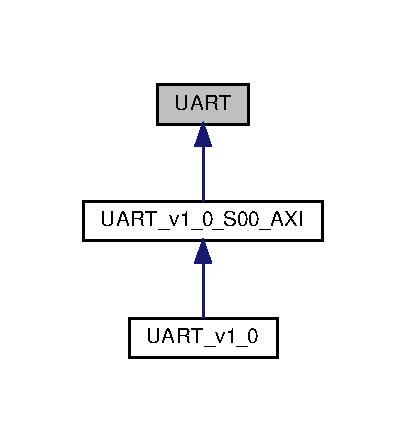
\includegraphics[width=195pt]{structUART__inherit__graph}
\end{center}
\end{figure}


\subsection{Detailed Description}
Stuttura che astrae un device \hyperlink{structUART}{U\+A\+RT} in kernel-\/mode. Contiene ciò che è necessario al funzionamento del driver. 

The documentation for this struct was generated from the following file\+:\begin{DoxyCompactItemize}
\item 
/media/saverio/\+O\+S/\+Users/\+Saverio/\+Desktop/\+S\+E/git/\+Michele/\+F\+P\+G\+A/\+U\+A\+R\+T/\+Driver/\+Con\+\_\+interrupt/\+K\+E\+R\+N\+E\+L\+\_\+\+M\+O\+D\+E/U\+A\+R\+T.\+h\end{DoxyCompactItemize}

\hypertarget{structUART__list}{}\section{U\+A\+R\+T\+\_\+list Struct Reference}
\label{structUART__list}\index{U\+A\+R\+T\+\_\+list@{U\+A\+R\+T\+\_\+list}}


Struttura dati per la gestione di più device \hyperlink{structUART}{U\+A\+RT} da parte del driver.  




{\ttfamily \#include $<$U\+A\+R\+T\+\_\+list.\+h$>$}



Collaboration diagram for U\+A\+R\+T\+\_\+list\+:
\nopagebreak
\begin{figure}[H]
\begin{center}
\leavevmode
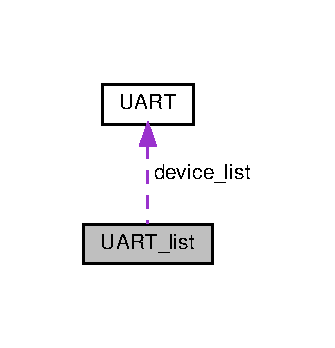
\includegraphics[width=161pt]{structUART__list__coll__graph}
\end{center}
\end{figure}
\subsection*{Data Fields}


\subsection{Detailed Description}
Struttura dati per la gestione di più device \hyperlink{structUART}{U\+A\+RT} da parte del driver. 

\subsection{Field Documentation}
\mbox{\Hypertarget{structUART__list_a170d1d78f27f6ab4c8badaaa4b3f2305}\label{structUART__list_a170d1d78f27f6ab4c8badaaa4b3f2305}} 
\index{U\+A\+R\+T\+\_\+list@{U\+A\+R\+T\+\_\+list}!device\+\_\+count@{device\+\_\+count}}
\index{device\+\_\+count@{device\+\_\+count}!U\+A\+R\+T\+\_\+list@{U\+A\+R\+T\+\_\+list}}
\subsubsection{\texorpdfstring{device\+\_\+count}{device\_count}}
{\footnotesize\ttfamily uint32\+\_\+t device\+\_\+count}

numero di device attivi e gestiti dal driver \mbox{\Hypertarget{structUART__list_a851af86c80724adf330596f12617066b}\label{structUART__list_a851af86c80724adf330596f12617066b}} 
\index{U\+A\+R\+T\+\_\+list@{U\+A\+R\+T\+\_\+list}!device\+\_\+list@{device\+\_\+list}}
\index{device\+\_\+list@{device\+\_\+list}!U\+A\+R\+T\+\_\+list@{U\+A\+R\+T\+\_\+list}}
\subsubsection{\texorpdfstring{device\+\_\+list}{device\_list}}
{\footnotesize\ttfamily \hyperlink{structUART}{U\+A\+RT}$\ast$$\ast$ device\+\_\+list}

array di puntatori a \hyperlink{structUART}{U\+A\+RT}, ciascuno dei quali si riferisce ad un device \mbox{\Hypertarget{structUART__list_aeff61809685e5df1b38aec1d871a49bb}\label{structUART__list_aeff61809685e5df1b38aec1d871a49bb}} 
\index{U\+A\+R\+T\+\_\+list@{U\+A\+R\+T\+\_\+list}!list\+\_\+size@{list\+\_\+size}}
\index{list\+\_\+size@{list\+\_\+size}!U\+A\+R\+T\+\_\+list@{U\+A\+R\+T\+\_\+list}}
\subsubsection{\texorpdfstring{list\+\_\+size}{list\_size}}
{\footnotesize\ttfamily uint32\+\_\+t list\+\_\+size}

dimensione della lista, ovvero il numero massimo di device gestibili 

The documentation for this struct was generated from the following file\+:\begin{DoxyCompactItemize}
\item 
/media/saverio/\+O\+S/\+Users/\+Saverio/\+Desktop/\+S\+E/git/\+Michele/\+F\+P\+G\+A/\+U\+A\+R\+T/\+Driver/\+Con\+\_\+interrupt/\+K\+E\+R\+N\+E\+L\+\_\+\+M\+O\+D\+E/\hyperlink{UART__list_8h}{U\+A\+R\+T\+\_\+list.\+h}\end{DoxyCompactItemize}

\hypertarget{classUART__v1__0}{}\section{U\+A\+R\+T\+\_\+v1\+\_\+0 Entity Reference}
\label{classUART__v1__0}\index{U\+A\+R\+T\+\_\+v1\+\_\+0@{U\+A\+R\+T\+\_\+v1\+\_\+0}}


Inheritance diagram for U\+A\+R\+T\+\_\+v1\+\_\+0\+:
\nopagebreak
\begin{figure}[H]
\begin{center}
\leavevmode
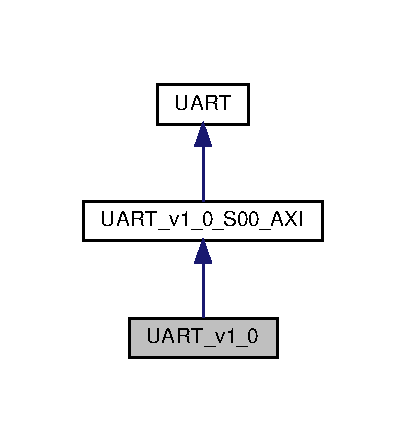
\includegraphics[width=195pt]{classUART__v1__0__inherit__graph}
\end{center}
\end{figure}


Collaboration diagram for U\+A\+R\+T\+\_\+v1\+\_\+0\+:
\nopagebreak
\begin{figure}[H]
\begin{center}
\leavevmode
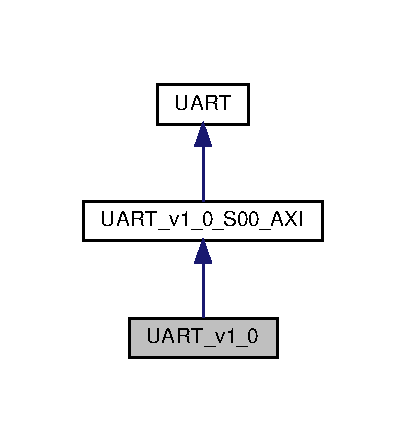
\includegraphics[width=195pt]{classUART__v1__0__coll__graph}
\end{center}
\end{figure}
\subsection*{Entities}
\begin{DoxyCompactItemize}
\item 
\hyperlink{classUART__v1__0_1_1arch__imp}{arch\+\_\+imp} architecture
\begin{DoxyCompactList}\small\item\em componente U\+A\+R\+T\+\_\+\+A\+X\+I\+\_\+\+S00  componente nel quale è incapsulato il componente \hyperlink{structUART}{U\+A\+RT} e la logica di gestione delle interruzioni. \end{DoxyCompactList}\end{DoxyCompactItemize}
\subsection*{Libraries}
 \begin{DoxyCompactItemize}
\item 
\mbox{\Hypertarget{classUART__v1__0_a0a6af6eef40212dbaf130d57ce711256}\label{classUART__v1__0_a0a6af6eef40212dbaf130d57ce711256}} 
\hyperlink{classUART__v1__0_a0a6af6eef40212dbaf130d57ce711256}{ieee} 
\begin{DoxyCompactList}\small\item\em Viene utilizzata la libreria I\+E\+EE. \end{DoxyCompactList}\end{DoxyCompactItemize}
\subsection*{Use Clauses}
 \begin{DoxyCompactItemize}
\item 
\mbox{\Hypertarget{classUART__v1__0_acd03516902501cd1c7296a98e22c6fcb}\label{classUART__v1__0_acd03516902501cd1c7296a98e22c6fcb}} 
\hyperlink{classUART__v1__0_acd03516902501cd1c7296a98e22c6fcb}{std\+\_\+logic\+\_\+1164}   
\begin{DoxyCompactList}\small\item\em Sono utilizzati i segnali della standard logic. \end{DoxyCompactList}\item 
\mbox{\Hypertarget{classUART__v1__0_a2edc34402b573437d5f25fa90ba4013e}\label{classUART__v1__0_a2edc34402b573437d5f25fa90ba4013e}} 
\hyperlink{classUART__v1__0_a2edc34402b573437d5f25fa90ba4013e}{numeric\+\_\+std}   
\begin{DoxyCompactList}\small\item\em Vengono utilizzate le funzioni numeriche. \end{DoxyCompactList}\end{DoxyCompactItemize}
\subsection*{Generics}
 \begin{DoxyCompactItemize}
\item 
\mbox{\Hypertarget{classUART__v1__0_af2979064a441fc814952a2a01b2e0bd3}\label{classUART__v1__0_af2979064a441fc814952a2a01b2e0bd3}} 
\hyperlink{classUART__v1__0_af2979064a441fc814952a2a01b2e0bd3}{baudrate} {\bfseries {\bfseries \textcolor{vhdlchar}{integer}\textcolor{vhdlchar}{ }\textcolor{vhdlchar}{ }\textcolor{vhdlchar}{\+:}\textcolor{vhdlchar}{=}\textcolor{vhdlchar}{ }\textcolor{vhdlchar}{ } \textcolor{vhdldigit}{9600} \textcolor{vhdlchar}{ }}}
\begin{DoxyCompactList}\small\item\em baudare trasmissione \end{DoxyCompactList}\item 
\mbox{\Hypertarget{classUART__v1__0_a378457a97325b4f40100f5b52b3dd886}\label{classUART__v1__0_a378457a97325b4f40100f5b52b3dd886}} 
\hyperlink{classUART__v1__0_a378457a97325b4f40100f5b52b3dd886}{clock\+\_\+freq} {\bfseries {\bfseries \textcolor{vhdlchar}{integer}\textcolor{vhdlchar}{ }\textcolor{vhdlchar}{ }\textcolor{vhdlchar}{\+:}\textcolor{vhdlchar}{=}\textcolor{vhdlchar}{ }\textcolor{vhdlchar}{ } \textcolor{vhdldigit}{50\+\_\+000\+\_\+000} \textcolor{vhdlchar}{ }}}
\begin{DoxyCompactList}\small\item\em frequenza clock ingresso \end{DoxyCompactList}\item 
\mbox{\Hypertarget{classUART__v1__0_afce7943994a4ddfa81f224225976a4c7}\label{classUART__v1__0_afce7943994a4ddfa81f224225976a4c7}} 
\hyperlink{classUART__v1__0_afce7943994a4ddfa81f224225976a4c7}{C\+\_\+\+S00\+\_\+\+A\+X\+I\+\_\+\+D\+A\+T\+A\+\_\+\+W\+I\+D\+TH} {\bfseries {\bfseries \textcolor{vhdlchar}{integer}\textcolor{vhdlchar}{ }\textcolor{vhdlchar}{ }\textcolor{vhdlchar}{\+:}\textcolor{vhdlchar}{=}\textcolor{vhdlchar}{ }\textcolor{vhdlchar}{ } \textcolor{vhdldigit}{32} \textcolor{vhdlchar}{ }}}
\item 
\mbox{\Hypertarget{classUART__v1__0_ab7787f274c76bb896ac98fdcfb570c65}\label{classUART__v1__0_ab7787f274c76bb896ac98fdcfb570c65}} 
\hyperlink{classUART__v1__0_ab7787f274c76bb896ac98fdcfb570c65}{C\+\_\+\+S00\+\_\+\+A\+X\+I\+\_\+\+A\+D\+D\+R\+\_\+\+W\+I\+D\+TH} {\bfseries {\bfseries \textcolor{vhdlchar}{integer}\textcolor{vhdlchar}{ }\textcolor{vhdlchar}{ }\textcolor{vhdlchar}{\+:}\textcolor{vhdlchar}{=}\textcolor{vhdlchar}{ }\textcolor{vhdlchar}{ } \textcolor{vhdldigit}{5} \textcolor{vhdlchar}{ }}}
\end{DoxyCompactItemize}
\subsection*{Ports}
 \begin{DoxyCompactItemize}
\item 
\mbox{\Hypertarget{classUART__v1__0_aa1eb566eeabe2a672e15ebb95aecc44f}\label{classUART__v1__0_aa1eb566eeabe2a672e15ebb95aecc44f}} 
\hyperlink{classUART__v1__0_aa1eb566eeabe2a672e15ebb95aecc44f}{tx}  {\bfseries {\bfseries \textcolor{vhdlchar}{out}\textcolor{vhdlchar}{ }}} {\bfseries \textcolor{vhdlchar}{std\+\_\+logic}\textcolor{vhdlchar}{ }} 
\begin{DoxyCompactList}\small\item\em linea uscita per la trasmissione \end{DoxyCompactList}\item 
\mbox{\Hypertarget{classUART__v1__0_a98ea5026beb91d6383a8a2aa2d69b32f}\label{classUART__v1__0_a98ea5026beb91d6383a8a2aa2d69b32f}} 
\hyperlink{classUART__v1__0_a98ea5026beb91d6383a8a2aa2d69b32f}{rx}  {\bfseries {\bfseries \textcolor{vhdlchar}{in}\textcolor{vhdlchar}{ }}} {\bfseries \textcolor{vhdlchar}{std\+\_\+logic}\textcolor{vhdlchar}{ }} 
\begin{DoxyCompactList}\small\item\em linea ingresso per la ricezione \end{DoxyCompactList}\item 
\mbox{\Hypertarget{classUART__v1__0_a5b78f3e3edfaf6e8ec79031b9e631e9d}\label{classUART__v1__0_a5b78f3e3edfaf6e8ec79031b9e631e9d}} 
\hyperlink{classUART__v1__0_a5b78f3e3edfaf6e8ec79031b9e631e9d}{interrupt}  {\bfseries {\bfseries \textcolor{vhdlchar}{out}\textcolor{vhdlchar}{ }}} {\bfseries \textcolor{vhdlchar}{std\+\_\+logic}\textcolor{vhdlchar}{ }} 
\begin{DoxyCompactList}\small\item\em segnale per richiede l\textquotesingle{}interrupt \end{DoxyCompactList}\item 
\mbox{\Hypertarget{classUART__v1__0_a037f9e3df8559bfd59db37bcba9cb7a8}\label{classUART__v1__0_a037f9e3df8559bfd59db37bcba9cb7a8}} 
\hyperlink{classUART__v1__0_a037f9e3df8559bfd59db37bcba9cb7a8}{s00\+\_\+axi\+\_\+aclk}  {\bfseries {\bfseries \textcolor{vhdlchar}{in}\textcolor{vhdlchar}{ }}} {\bfseries \textcolor{vhdlchar}{std\+\_\+logic}\textcolor{vhdlchar}{ }} 
\item 
\mbox{\Hypertarget{classUART__v1__0_a8249c106fbd80196dcad2666c9f0b3fc}\label{classUART__v1__0_a8249c106fbd80196dcad2666c9f0b3fc}} 
\hyperlink{classUART__v1__0_a8249c106fbd80196dcad2666c9f0b3fc}{s00\+\_\+axi\+\_\+aresetn}  {\bfseries {\bfseries \textcolor{vhdlchar}{in}\textcolor{vhdlchar}{ }}} {\bfseries \textcolor{vhdlchar}{std\+\_\+logic}\textcolor{vhdlchar}{ }} 
\item 
\mbox{\Hypertarget{classUART__v1__0_a9fe80d3cc7f862afb670536e4e05dbeb}\label{classUART__v1__0_a9fe80d3cc7f862afb670536e4e05dbeb}} 
\hyperlink{classUART__v1__0_a9fe80d3cc7f862afb670536e4e05dbeb}{s00\+\_\+axi\+\_\+awaddr}  {\bfseries {\bfseries \textcolor{vhdlchar}{in}\textcolor{vhdlchar}{ }}} {\bfseries \textcolor{vhdlchar}{std\+\_\+logic\+\_\+vector}\textcolor{vhdlchar}{ }\textcolor{vhdlchar}{(}\textcolor{vhdlchar}{ }\textcolor{vhdlchar}{ }\textcolor{vhdlchar}{ }\textcolor{vhdlchar}{ }\textcolor{vhdlchar}{C\+\_\+\+S00\+\_\+\+A\+X\+I\+\_\+\+A\+D\+D\+R\+\_\+\+W\+I\+D\+TH}\textcolor{vhdlchar}{-\/}\textcolor{vhdlchar}{ } \textcolor{vhdldigit}{1} \textcolor{vhdlchar}{ }\textcolor{vhdlchar}{downto}\textcolor{vhdlchar}{ }\textcolor{vhdlchar}{ } \textcolor{vhdldigit}{0} \textcolor{vhdlchar}{ }\textcolor{vhdlchar}{)}\textcolor{vhdlchar}{ }} 
\item 
\mbox{\Hypertarget{classUART__v1__0_a719659c1addef5432978cc949d9e10ed}\label{classUART__v1__0_a719659c1addef5432978cc949d9e10ed}} 
\hyperlink{classUART__v1__0_a719659c1addef5432978cc949d9e10ed}{s00\+\_\+axi\+\_\+awprot}  {\bfseries {\bfseries \textcolor{vhdlchar}{in}\textcolor{vhdlchar}{ }}} {\bfseries \textcolor{vhdlchar}{std\+\_\+logic\+\_\+vector}\textcolor{vhdlchar}{ }\textcolor{vhdlchar}{(}\textcolor{vhdlchar}{ }\textcolor{vhdlchar}{ } \textcolor{vhdldigit}{2} \textcolor{vhdlchar}{ }\textcolor{vhdlchar}{downto}\textcolor{vhdlchar}{ }\textcolor{vhdlchar}{ } \textcolor{vhdldigit}{0} \textcolor{vhdlchar}{ }\textcolor{vhdlchar}{)}\textcolor{vhdlchar}{ }} 
\item 
\mbox{\Hypertarget{classUART__v1__0_a45aa02a72ae1a8389346d47173c60ed0}\label{classUART__v1__0_a45aa02a72ae1a8389346d47173c60ed0}} 
\hyperlink{classUART__v1__0_a45aa02a72ae1a8389346d47173c60ed0}{s00\+\_\+axi\+\_\+awvalid}  {\bfseries {\bfseries \textcolor{vhdlchar}{in}\textcolor{vhdlchar}{ }}} {\bfseries \textcolor{vhdlchar}{std\+\_\+logic}\textcolor{vhdlchar}{ }} 
\item 
\mbox{\Hypertarget{classUART__v1__0_ad0a1f71502d91a45dbc6c365f85c6566}\label{classUART__v1__0_ad0a1f71502d91a45dbc6c365f85c6566}} 
\hyperlink{classUART__v1__0_ad0a1f71502d91a45dbc6c365f85c6566}{s00\+\_\+axi\+\_\+awready}  {\bfseries {\bfseries \textcolor{vhdlchar}{out}\textcolor{vhdlchar}{ }}} {\bfseries \textcolor{vhdlchar}{std\+\_\+logic}\textcolor{vhdlchar}{ }} 
\item 
\mbox{\Hypertarget{classUART__v1__0_ae2b15b55ee463fd9dd030ee29db6bb17}\label{classUART__v1__0_ae2b15b55ee463fd9dd030ee29db6bb17}} 
\hyperlink{classUART__v1__0_ae2b15b55ee463fd9dd030ee29db6bb17}{s00\+\_\+axi\+\_\+wdata}  {\bfseries {\bfseries \textcolor{vhdlchar}{in}\textcolor{vhdlchar}{ }}} {\bfseries \textcolor{vhdlchar}{std\+\_\+logic\+\_\+vector}\textcolor{vhdlchar}{ }\textcolor{vhdlchar}{(}\textcolor{vhdlchar}{ }\textcolor{vhdlchar}{ }\textcolor{vhdlchar}{ }\textcolor{vhdlchar}{ }\textcolor{vhdlchar}{C\+\_\+\+S00\+\_\+\+A\+X\+I\+\_\+\+D\+A\+T\+A\+\_\+\+W\+I\+D\+TH}\textcolor{vhdlchar}{-\/}\textcolor{vhdlchar}{ } \textcolor{vhdldigit}{1} \textcolor{vhdlchar}{ }\textcolor{vhdlchar}{downto}\textcolor{vhdlchar}{ }\textcolor{vhdlchar}{ } \textcolor{vhdldigit}{0} \textcolor{vhdlchar}{ }\textcolor{vhdlchar}{)}\textcolor{vhdlchar}{ }} 
\item 
\mbox{\Hypertarget{classUART__v1__0_a120924bc3fd5fd10ec0f96e19c3f4904}\label{classUART__v1__0_a120924bc3fd5fd10ec0f96e19c3f4904}} 
\hyperlink{classUART__v1__0_a120924bc3fd5fd10ec0f96e19c3f4904}{s00\+\_\+axi\+\_\+wstrb}  {\bfseries {\bfseries \textcolor{vhdlchar}{in}\textcolor{vhdlchar}{ }}} {\bfseries \textcolor{vhdlchar}{std\+\_\+logic\+\_\+vector}\textcolor{vhdlchar}{ }\textcolor{vhdlchar}{(}\textcolor{vhdlchar}{ }\textcolor{vhdlchar}{(}\textcolor{vhdlchar}{ }\textcolor{vhdlchar}{ }\textcolor{vhdlchar}{ }\textcolor{vhdlchar}{ }\textcolor{vhdlchar}{C\+\_\+\+S00\+\_\+\+A\+X\+I\+\_\+\+D\+A\+T\+A\+\_\+\+W\+I\+D\+TH}\textcolor{vhdlchar}{/}\textcolor{vhdlchar}{ } \textcolor{vhdldigit}{8} \textcolor{vhdlchar}{ }\textcolor{vhdlchar}{)}\textcolor{vhdlchar}{ }\textcolor{vhdlchar}{-\/}\textcolor{vhdlchar}{ } \textcolor{vhdldigit}{1} \textcolor{vhdlchar}{ }\textcolor{vhdlchar}{downto}\textcolor{vhdlchar}{ }\textcolor{vhdlchar}{ } \textcolor{vhdldigit}{0} \textcolor{vhdlchar}{ }\textcolor{vhdlchar}{)}\textcolor{vhdlchar}{ }} 
\item 
\mbox{\Hypertarget{classUART__v1__0_a24e90907193647007d2947353740114d}\label{classUART__v1__0_a24e90907193647007d2947353740114d}} 
\hyperlink{classUART__v1__0_a24e90907193647007d2947353740114d}{s00\+\_\+axi\+\_\+wvalid}  {\bfseries {\bfseries \textcolor{vhdlchar}{in}\textcolor{vhdlchar}{ }}} {\bfseries \textcolor{vhdlchar}{std\+\_\+logic}\textcolor{vhdlchar}{ }} 
\item 
\mbox{\Hypertarget{classUART__v1__0_a3fc60abc0cfbfa90003a83bffdd476c4}\label{classUART__v1__0_a3fc60abc0cfbfa90003a83bffdd476c4}} 
\hyperlink{classUART__v1__0_a3fc60abc0cfbfa90003a83bffdd476c4}{s00\+\_\+axi\+\_\+wready}  {\bfseries {\bfseries \textcolor{vhdlchar}{out}\textcolor{vhdlchar}{ }}} {\bfseries \textcolor{vhdlchar}{std\+\_\+logic}\textcolor{vhdlchar}{ }} 
\item 
\mbox{\Hypertarget{classUART__v1__0_af8799be946d3f5354263e7deb15f94f1}\label{classUART__v1__0_af8799be946d3f5354263e7deb15f94f1}} 
\hyperlink{classUART__v1__0_af8799be946d3f5354263e7deb15f94f1}{s00\+\_\+axi\+\_\+bresp}  {\bfseries {\bfseries \textcolor{vhdlchar}{out}\textcolor{vhdlchar}{ }}} {\bfseries \textcolor{vhdlchar}{std\+\_\+logic\+\_\+vector}\textcolor{vhdlchar}{ }\textcolor{vhdlchar}{(}\textcolor{vhdlchar}{ }\textcolor{vhdlchar}{ } \textcolor{vhdldigit}{1} \textcolor{vhdlchar}{ }\textcolor{vhdlchar}{downto}\textcolor{vhdlchar}{ }\textcolor{vhdlchar}{ } \textcolor{vhdldigit}{0} \textcolor{vhdlchar}{ }\textcolor{vhdlchar}{)}\textcolor{vhdlchar}{ }} 
\item 
\mbox{\Hypertarget{classUART__v1__0_a5110b7dd4fb9548a2aab88f50dbe1d5e}\label{classUART__v1__0_a5110b7dd4fb9548a2aab88f50dbe1d5e}} 
\hyperlink{classUART__v1__0_a5110b7dd4fb9548a2aab88f50dbe1d5e}{s00\+\_\+axi\+\_\+bvalid}  {\bfseries {\bfseries \textcolor{vhdlchar}{out}\textcolor{vhdlchar}{ }}} {\bfseries \textcolor{vhdlchar}{std\+\_\+logic}\textcolor{vhdlchar}{ }} 
\item 
\mbox{\Hypertarget{classUART__v1__0_a1ef2019b0613bc23d4829eeeb24eb98d}\label{classUART__v1__0_a1ef2019b0613bc23d4829eeeb24eb98d}} 
\hyperlink{classUART__v1__0_a1ef2019b0613bc23d4829eeeb24eb98d}{s00\+\_\+axi\+\_\+bready}  {\bfseries {\bfseries \textcolor{vhdlchar}{in}\textcolor{vhdlchar}{ }}} {\bfseries \textcolor{vhdlchar}{std\+\_\+logic}\textcolor{vhdlchar}{ }} 
\item 
\mbox{\Hypertarget{classUART__v1__0_af70a86336cd6505064e45b69f4623939}\label{classUART__v1__0_af70a86336cd6505064e45b69f4623939}} 
\hyperlink{classUART__v1__0_af70a86336cd6505064e45b69f4623939}{s00\+\_\+axi\+\_\+araddr}  {\bfseries {\bfseries \textcolor{vhdlchar}{in}\textcolor{vhdlchar}{ }}} {\bfseries \textcolor{vhdlchar}{std\+\_\+logic\+\_\+vector}\textcolor{vhdlchar}{ }\textcolor{vhdlchar}{(}\textcolor{vhdlchar}{ }\textcolor{vhdlchar}{ }\textcolor{vhdlchar}{ }\textcolor{vhdlchar}{ }\textcolor{vhdlchar}{C\+\_\+\+S00\+\_\+\+A\+X\+I\+\_\+\+A\+D\+D\+R\+\_\+\+W\+I\+D\+TH}\textcolor{vhdlchar}{-\/}\textcolor{vhdlchar}{ } \textcolor{vhdldigit}{1} \textcolor{vhdlchar}{ }\textcolor{vhdlchar}{downto}\textcolor{vhdlchar}{ }\textcolor{vhdlchar}{ } \textcolor{vhdldigit}{0} \textcolor{vhdlchar}{ }\textcolor{vhdlchar}{)}\textcolor{vhdlchar}{ }} 
\item 
\mbox{\Hypertarget{classUART__v1__0_adc648df07895bf808b8c721e1dc6811b}\label{classUART__v1__0_adc648df07895bf808b8c721e1dc6811b}} 
\hyperlink{classUART__v1__0_adc648df07895bf808b8c721e1dc6811b}{s00\+\_\+axi\+\_\+arprot}  {\bfseries {\bfseries \textcolor{vhdlchar}{in}\textcolor{vhdlchar}{ }}} {\bfseries \textcolor{vhdlchar}{std\+\_\+logic\+\_\+vector}\textcolor{vhdlchar}{ }\textcolor{vhdlchar}{(}\textcolor{vhdlchar}{ }\textcolor{vhdlchar}{ } \textcolor{vhdldigit}{2} \textcolor{vhdlchar}{ }\textcolor{vhdlchar}{downto}\textcolor{vhdlchar}{ }\textcolor{vhdlchar}{ } \textcolor{vhdldigit}{0} \textcolor{vhdlchar}{ }\textcolor{vhdlchar}{)}\textcolor{vhdlchar}{ }} 
\item 
\mbox{\Hypertarget{classUART__v1__0_a94b78b2ae3cd13860f15afbdfb199e44}\label{classUART__v1__0_a94b78b2ae3cd13860f15afbdfb199e44}} 
\hyperlink{classUART__v1__0_a94b78b2ae3cd13860f15afbdfb199e44}{s00\+\_\+axi\+\_\+arvalid}  {\bfseries {\bfseries \textcolor{vhdlchar}{in}\textcolor{vhdlchar}{ }}} {\bfseries \textcolor{vhdlchar}{std\+\_\+logic}\textcolor{vhdlchar}{ }} 
\item 
\mbox{\Hypertarget{classUART__v1__0_ad35bd95f3352ff8dbdaea55205a98e53}\label{classUART__v1__0_ad35bd95f3352ff8dbdaea55205a98e53}} 
\hyperlink{classUART__v1__0_ad35bd95f3352ff8dbdaea55205a98e53}{s00\+\_\+axi\+\_\+arready}  {\bfseries {\bfseries \textcolor{vhdlchar}{out}\textcolor{vhdlchar}{ }}} {\bfseries \textcolor{vhdlchar}{std\+\_\+logic}\textcolor{vhdlchar}{ }} 
\item 
\mbox{\Hypertarget{classUART__v1__0_ad2655fadb987e0487c428aca187b55d0}\label{classUART__v1__0_ad2655fadb987e0487c428aca187b55d0}} 
\hyperlink{classUART__v1__0_ad2655fadb987e0487c428aca187b55d0}{s00\+\_\+axi\+\_\+rdata}  {\bfseries {\bfseries \textcolor{vhdlchar}{out}\textcolor{vhdlchar}{ }}} {\bfseries \textcolor{vhdlchar}{std\+\_\+logic\+\_\+vector}\textcolor{vhdlchar}{ }\textcolor{vhdlchar}{(}\textcolor{vhdlchar}{ }\textcolor{vhdlchar}{ }\textcolor{vhdlchar}{ }\textcolor{vhdlchar}{ }\textcolor{vhdlchar}{C\+\_\+\+S00\+\_\+\+A\+X\+I\+\_\+\+D\+A\+T\+A\+\_\+\+W\+I\+D\+TH}\textcolor{vhdlchar}{-\/}\textcolor{vhdlchar}{ } \textcolor{vhdldigit}{1} \textcolor{vhdlchar}{ }\textcolor{vhdlchar}{downto}\textcolor{vhdlchar}{ }\textcolor{vhdlchar}{ } \textcolor{vhdldigit}{0} \textcolor{vhdlchar}{ }\textcolor{vhdlchar}{)}\textcolor{vhdlchar}{ }} 
\item 
\mbox{\Hypertarget{classUART__v1__0_a1acee955f50f71e5595a03c6ca301cf0}\label{classUART__v1__0_a1acee955f50f71e5595a03c6ca301cf0}} 
\hyperlink{classUART__v1__0_a1acee955f50f71e5595a03c6ca301cf0}{s00\+\_\+axi\+\_\+rresp}  {\bfseries {\bfseries \textcolor{vhdlchar}{out}\textcolor{vhdlchar}{ }}} {\bfseries \textcolor{vhdlchar}{std\+\_\+logic\+\_\+vector}\textcolor{vhdlchar}{ }\textcolor{vhdlchar}{(}\textcolor{vhdlchar}{ }\textcolor{vhdlchar}{ } \textcolor{vhdldigit}{1} \textcolor{vhdlchar}{ }\textcolor{vhdlchar}{downto}\textcolor{vhdlchar}{ }\textcolor{vhdlchar}{ } \textcolor{vhdldigit}{0} \textcolor{vhdlchar}{ }\textcolor{vhdlchar}{)}\textcolor{vhdlchar}{ }} 
\item 
\mbox{\Hypertarget{classUART__v1__0_af180911f7eb262e530e26865bc97aa0b}\label{classUART__v1__0_af180911f7eb262e530e26865bc97aa0b}} 
\hyperlink{classUART__v1__0_af180911f7eb262e530e26865bc97aa0b}{s00\+\_\+axi\+\_\+rvalid}  {\bfseries {\bfseries \textcolor{vhdlchar}{out}\textcolor{vhdlchar}{ }}} {\bfseries \textcolor{vhdlchar}{std\+\_\+logic}\textcolor{vhdlchar}{ }} 
\item 
\mbox{\Hypertarget{classUART__v1__0_a8b82eb165d7024f6c7b25646f6ebdd4d}\label{classUART__v1__0_a8b82eb165d7024f6c7b25646f6ebdd4d}} 
\hyperlink{classUART__v1__0_a8b82eb165d7024f6c7b25646f6ebdd4d}{s00\+\_\+axi\+\_\+rready}  {\bfseries {\bfseries \textcolor{vhdlchar}{in}\textcolor{vhdlchar}{ }}} {\bfseries \textcolor{vhdlchar}{std\+\_\+logic}\textcolor{vhdlchar}{ }} 
\end{DoxyCompactItemize}


The documentation for this class was generated from the following file\+:\begin{DoxyCompactItemize}
\item 
/media/saverio/\+O\+S/\+Users/\+Saverio/\+Desktop/\+S\+E/git/\+Andrea/\+F\+P\+G\+A/ip\+\_\+repo/\+U\+A\+R\+T\+\_\+1.\+0/hdl/\hyperlink{UART__v1__0_8vhd}{U\+A\+R\+T\+\_\+v1\+\_\+0.\+vhd}\end{DoxyCompactItemize}

\hypertarget{classUART__v1__0__S00__AXI}{}\section{U\+A\+R\+T\+\_\+v1\+\_\+0\+\_\+\+S00\+\_\+\+A\+XI Entity Reference}
\label{classUART__v1__0__S00__AXI}\index{U\+A\+R\+T\+\_\+v1\+\_\+0\+\_\+\+S00\+\_\+\+A\+XI@{U\+A\+R\+T\+\_\+v1\+\_\+0\+\_\+\+S00\+\_\+\+A\+XI}}


Inheritance diagram for U\+A\+R\+T\+\_\+v1\+\_\+0\+\_\+\+S00\+\_\+\+A\+XI\+:\nopagebreak
\begin{figure}[H]
\begin{center}
\leavevmode
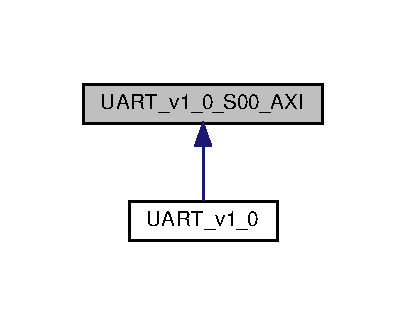
\includegraphics[width=195pt]{classUART__v1__0__S00__AXI__inherit__graph}
\end{center}
\end{figure}


Collaboration diagram for U\+A\+R\+T\+\_\+v1\+\_\+0\+\_\+\+S00\+\_\+\+A\+XI\+:\nopagebreak
\begin{figure}[H]
\begin{center}
\leavevmode
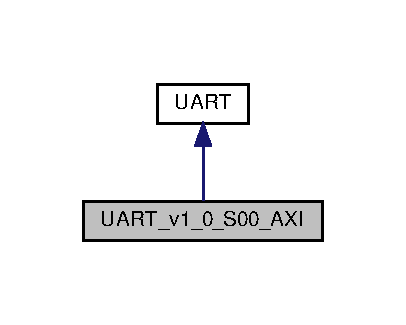
\includegraphics[width=195pt]{classUART__v1__0__S00__AXI__coll__graph}
\end{center}
\end{figure}
\subsection*{Entities}
\begin{DoxyCompactItemize}
\item 
\hyperlink{classUART__v1__0__S00__AXI_1_1arch__imp}{arch\+\_\+imp} architecture
\end{DoxyCompactItemize}
\subsection*{Libraries}
 \begin{DoxyCompactItemize}
\item 
\mbox{\Hypertarget{classUART__v1__0__S00__AXI_a0a6af6eef40212dbaf130d57ce711256}\label{classUART__v1__0__S00__AXI_a0a6af6eef40212dbaf130d57ce711256}} 
\hyperlink{classUART__v1__0__S00__AXI_a0a6af6eef40212dbaf130d57ce711256}{ieee} 
\begin{DoxyCompactList}\small\item\em Viene utilizzata la libreria I\+E\+EE. \end{DoxyCompactList}\end{DoxyCompactItemize}
\subsection*{Use Clauses}
 \begin{DoxyCompactItemize}
\item 
\mbox{\Hypertarget{classUART__v1__0__S00__AXI_acd03516902501cd1c7296a98e22c6fcb}\label{classUART__v1__0__S00__AXI_acd03516902501cd1c7296a98e22c6fcb}} 
\hyperlink{classUART__v1__0__S00__AXI_acd03516902501cd1c7296a98e22c6fcb}{std\+\_\+logic\+\_\+1164}   
\begin{DoxyCompactList}\small\item\em Sono utilizzati i segnali della standard logic. \end{DoxyCompactList}\item 
\mbox{\Hypertarget{classUART__v1__0__S00__AXI_a2edc34402b573437d5f25fa90ba4013e}\label{classUART__v1__0__S00__AXI_a2edc34402b573437d5f25fa90ba4013e}} 
\hyperlink{classUART__v1__0__S00__AXI_a2edc34402b573437d5f25fa90ba4013e}{numeric\+\_\+std}   
\begin{DoxyCompactList}\small\item\em Vengono utilizzate le funzioni numeriche. \end{DoxyCompactList}\item 
\mbox{\Hypertarget{classUART__v1__0__S00__AXI_acb2d98d781f19c8f5f4109576ec45502}\label{classUART__v1__0__S00__AXI_acb2d98d781f19c8f5f4109576ec45502}} 
\hyperlink{classUART__v1__0__S00__AXI_acb2d98d781f19c8f5f4109576ec45502}{std\+\_\+logic\+\_\+misc}   
\begin{DoxyCompactList}\small\item\em libreria necessaria per la funzione or\+\_\+reduce \end{DoxyCompactList}\end{DoxyCompactItemize}
\subsection*{Generics}
 \begin{DoxyCompactItemize}
\item 
\mbox{\Hypertarget{classUART__v1__0__S00__AXI_af2979064a441fc814952a2a01b2e0bd3}\label{classUART__v1__0__S00__AXI_af2979064a441fc814952a2a01b2e0bd3}} 
\hyperlink{classUART__v1__0__S00__AXI_af2979064a441fc814952a2a01b2e0bd3}{baudrate} {\bfseries {\bfseries \textcolor{vhdlchar}{integer}\textcolor{vhdlchar}{ }\textcolor{vhdlchar}{ }\textcolor{vhdlchar}{\+:}\textcolor{vhdlchar}{=}\textcolor{vhdlchar}{ }\textcolor{vhdlchar}{ } \textcolor{vhdldigit}{9600} \textcolor{vhdlchar}{ }}}
\item 
\mbox{\Hypertarget{classUART__v1__0__S00__AXI_a378457a97325b4f40100f5b52b3dd886}\label{classUART__v1__0__S00__AXI_a378457a97325b4f40100f5b52b3dd886}} 
\hyperlink{classUART__v1__0__S00__AXI_a378457a97325b4f40100f5b52b3dd886}{clock\+\_\+freq} {\bfseries {\bfseries \textcolor{vhdlchar}{integer}\textcolor{vhdlchar}{ }\textcolor{vhdlchar}{ }\textcolor{vhdlchar}{\+:}\textcolor{vhdlchar}{=}\textcolor{vhdlchar}{ }\textcolor{vhdlchar}{ } \textcolor{vhdldigit}{50\+\_\+000\+\_\+000} \textcolor{vhdlchar}{ }}}
\item 
\mbox{\Hypertarget{classUART__v1__0__S00__AXI_a0fad312acd1f302ce7de30c5658df0bd}\label{classUART__v1__0__S00__AXI_a0fad312acd1f302ce7de30c5658df0bd}} 
\hyperlink{classUART__v1__0__S00__AXI_a0fad312acd1f302ce7de30c5658df0bd}{C\+\_\+\+S\+\_\+\+A\+X\+I\+\_\+\+D\+A\+T\+A\+\_\+\+W\+I\+D\+TH} {\bfseries {\bfseries \textcolor{vhdlchar}{integer}\textcolor{vhdlchar}{ }\textcolor{vhdlchar}{ }\textcolor{vhdlchar}{\+:}\textcolor{vhdlchar}{=}\textcolor{vhdlchar}{ }\textcolor{vhdlchar}{ } \textcolor{vhdldigit}{32} \textcolor{vhdlchar}{ }}}
\item 
\mbox{\Hypertarget{classUART__v1__0__S00__AXI_a9abff2eaa069440f3b7d9e9937d5ee8e}\label{classUART__v1__0__S00__AXI_a9abff2eaa069440f3b7d9e9937d5ee8e}} 
\hyperlink{classUART__v1__0__S00__AXI_a9abff2eaa069440f3b7d9e9937d5ee8e}{C\+\_\+\+S\+\_\+\+A\+X\+I\+\_\+\+A\+D\+D\+R\+\_\+\+W\+I\+D\+TH} {\bfseries {\bfseries \textcolor{vhdlchar}{integer}\textcolor{vhdlchar}{ }\textcolor{vhdlchar}{ }\textcolor{vhdlchar}{\+:}\textcolor{vhdlchar}{=}\textcolor{vhdlchar}{ }\textcolor{vhdlchar}{ } \textcolor{vhdldigit}{5} \textcolor{vhdlchar}{ }}}
\end{DoxyCompactItemize}
\subsection*{Ports}
 \begin{DoxyCompactItemize}
\item 
\mbox{\Hypertarget{classUART__v1__0__S00__AXI_aa1eb566eeabe2a672e15ebb95aecc44f}\label{classUART__v1__0__S00__AXI_aa1eb566eeabe2a672e15ebb95aecc44f}} 
\hyperlink{classUART__v1__0__S00__AXI_aa1eb566eeabe2a672e15ebb95aecc44f}{tx}  {\bfseries {\bfseries \textcolor{vhdlchar}{out}\textcolor{vhdlchar}{ }}} {\bfseries \textcolor{vhdlchar}{std\+\_\+logic}\textcolor{vhdlchar}{ }} 
\item 
\mbox{\Hypertarget{classUART__v1__0__S00__AXI_a98ea5026beb91d6383a8a2aa2d69b32f}\label{classUART__v1__0__S00__AXI_a98ea5026beb91d6383a8a2aa2d69b32f}} 
\hyperlink{classUART__v1__0__S00__AXI_a98ea5026beb91d6383a8a2aa2d69b32f}{rx}  {\bfseries {\bfseries \textcolor{vhdlchar}{in}\textcolor{vhdlchar}{ }}} {\bfseries \textcolor{vhdlchar}{std\+\_\+logic}\textcolor{vhdlchar}{ }} 
\item 
\mbox{\Hypertarget{classUART__v1__0__S00__AXI_a5b78f3e3edfaf6e8ec79031b9e631e9d}\label{classUART__v1__0__S00__AXI_a5b78f3e3edfaf6e8ec79031b9e631e9d}} 
\hyperlink{classUART__v1__0__S00__AXI_a5b78f3e3edfaf6e8ec79031b9e631e9d}{interrupt}  {\bfseries {\bfseries \textcolor{vhdlchar}{out}\textcolor{vhdlchar}{ }}} {\bfseries \textcolor{vhdlchar}{std\+\_\+logic}\textcolor{vhdlchar}{ }} 
\item 
\mbox{\Hypertarget{classUART__v1__0__S00__AXI_a3f54d782a88290bdaa6baffd7cd84ab4}\label{classUART__v1__0__S00__AXI_a3f54d782a88290bdaa6baffd7cd84ab4}} 
\hyperlink{classUART__v1__0__S00__AXI_a3f54d782a88290bdaa6baffd7cd84ab4}{S\+\_\+\+A\+X\+I\+\_\+\+A\+C\+LK}  {\bfseries {\bfseries \textcolor{vhdlchar}{in}\textcolor{vhdlchar}{ }}} {\bfseries \textcolor{vhdlchar}{std\+\_\+logic}\textcolor{vhdlchar}{ }} 
\item 
\mbox{\Hypertarget{classUART__v1__0__S00__AXI_a089b396e17dee353ccc7d5389dda5532}\label{classUART__v1__0__S00__AXI_a089b396e17dee353ccc7d5389dda5532}} 
\hyperlink{classUART__v1__0__S00__AXI_a089b396e17dee353ccc7d5389dda5532}{S\+\_\+\+A\+X\+I\+\_\+\+A\+R\+E\+S\+E\+TN}  {\bfseries {\bfseries \textcolor{vhdlchar}{in}\textcolor{vhdlchar}{ }}} {\bfseries \textcolor{vhdlchar}{std\+\_\+logic}\textcolor{vhdlchar}{ }} 
\item 
\mbox{\Hypertarget{classUART__v1__0__S00__AXI_a61cc7b190ba9d540e56941330e4a0883}\label{classUART__v1__0__S00__AXI_a61cc7b190ba9d540e56941330e4a0883}} 
\hyperlink{classUART__v1__0__S00__AXI_a61cc7b190ba9d540e56941330e4a0883}{S\+\_\+\+A\+X\+I\+\_\+\+A\+W\+A\+D\+DR}  {\bfseries {\bfseries \textcolor{vhdlchar}{in}\textcolor{vhdlchar}{ }}} {\bfseries \textcolor{vhdlchar}{std\+\_\+logic\+\_\+vector}\textcolor{vhdlchar}{ }\textcolor{vhdlchar}{(}\textcolor{vhdlchar}{ }\textcolor{vhdlchar}{ }\textcolor{vhdlchar}{ }\textcolor{vhdlchar}{ }\textcolor{vhdlchar}{C\+\_\+\+S\+\_\+\+A\+X\+I\+\_\+\+A\+D\+D\+R\+\_\+\+W\+I\+D\+TH}\textcolor{vhdlchar}{-\/}\textcolor{vhdlchar}{ } \textcolor{vhdldigit}{1} \textcolor{vhdlchar}{ }\textcolor{vhdlchar}{downto}\textcolor{vhdlchar}{ }\textcolor{vhdlchar}{ } \textcolor{vhdldigit}{0} \textcolor{vhdlchar}{ }\textcolor{vhdlchar}{)}\textcolor{vhdlchar}{ }} 
\item 
\mbox{\Hypertarget{classUART__v1__0__S00__AXI_a459abcd98567ad24261377eed899593a}\label{classUART__v1__0__S00__AXI_a459abcd98567ad24261377eed899593a}} 
\hyperlink{classUART__v1__0__S00__AXI_a459abcd98567ad24261377eed899593a}{S\+\_\+\+A\+X\+I\+\_\+\+A\+W\+P\+R\+OT}  {\bfseries {\bfseries \textcolor{vhdlchar}{in}\textcolor{vhdlchar}{ }}} {\bfseries \textcolor{vhdlchar}{std\+\_\+logic\+\_\+vector}\textcolor{vhdlchar}{ }\textcolor{vhdlchar}{(}\textcolor{vhdlchar}{ }\textcolor{vhdlchar}{ } \textcolor{vhdldigit}{2} \textcolor{vhdlchar}{ }\textcolor{vhdlchar}{downto}\textcolor{vhdlchar}{ }\textcolor{vhdlchar}{ } \textcolor{vhdldigit}{0} \textcolor{vhdlchar}{ }\textcolor{vhdlchar}{)}\textcolor{vhdlchar}{ }} 
\item 
\mbox{\Hypertarget{classUART__v1__0__S00__AXI_af1f1cbf67bf647ba58353c261719a3a0}\label{classUART__v1__0__S00__AXI_af1f1cbf67bf647ba58353c261719a3a0}} 
\hyperlink{classUART__v1__0__S00__AXI_af1f1cbf67bf647ba58353c261719a3a0}{S\+\_\+\+A\+X\+I\+\_\+\+A\+W\+V\+A\+L\+ID}  {\bfseries {\bfseries \textcolor{vhdlchar}{in}\textcolor{vhdlchar}{ }}} {\bfseries \textcolor{vhdlchar}{std\+\_\+logic}\textcolor{vhdlchar}{ }} 
\item 
\mbox{\Hypertarget{classUART__v1__0__S00__AXI_ac04aab5cc834e762e893e061016921c6}\label{classUART__v1__0__S00__AXI_ac04aab5cc834e762e893e061016921c6}} 
\hyperlink{classUART__v1__0__S00__AXI_ac04aab5cc834e762e893e061016921c6}{S\+\_\+\+A\+X\+I\+\_\+\+A\+W\+R\+E\+A\+DY}  {\bfseries {\bfseries \textcolor{vhdlchar}{out}\textcolor{vhdlchar}{ }}} {\bfseries \textcolor{vhdlchar}{std\+\_\+logic}\textcolor{vhdlchar}{ }} 
\item 
\mbox{\Hypertarget{classUART__v1__0__S00__AXI_a292e5db13719faf3a8b3aab091773467}\label{classUART__v1__0__S00__AXI_a292e5db13719faf3a8b3aab091773467}} 
\hyperlink{classUART__v1__0__S00__AXI_a292e5db13719faf3a8b3aab091773467}{S\+\_\+\+A\+X\+I\+\_\+\+W\+D\+A\+TA}  {\bfseries {\bfseries \textcolor{vhdlchar}{in}\textcolor{vhdlchar}{ }}} {\bfseries \textcolor{vhdlchar}{std\+\_\+logic\+\_\+vector}\textcolor{vhdlchar}{ }\textcolor{vhdlchar}{(}\textcolor{vhdlchar}{ }\textcolor{vhdlchar}{ }\textcolor{vhdlchar}{ }\textcolor{vhdlchar}{ }\textcolor{vhdlchar}{C\+\_\+\+S\+\_\+\+A\+X\+I\+\_\+\+D\+A\+T\+A\+\_\+\+W\+I\+D\+TH}\textcolor{vhdlchar}{-\/}\textcolor{vhdlchar}{ } \textcolor{vhdldigit}{1} \textcolor{vhdlchar}{ }\textcolor{vhdlchar}{downto}\textcolor{vhdlchar}{ }\textcolor{vhdlchar}{ } \textcolor{vhdldigit}{0} \textcolor{vhdlchar}{ }\textcolor{vhdlchar}{)}\textcolor{vhdlchar}{ }} 
\item 
\mbox{\Hypertarget{classUART__v1__0__S00__AXI_accd8e04b79540b57ab15fee1cb6c04f5}\label{classUART__v1__0__S00__AXI_accd8e04b79540b57ab15fee1cb6c04f5}} 
\hyperlink{classUART__v1__0__S00__AXI_accd8e04b79540b57ab15fee1cb6c04f5}{S\+\_\+\+A\+X\+I\+\_\+\+W\+S\+T\+RB}  {\bfseries {\bfseries \textcolor{vhdlchar}{in}\textcolor{vhdlchar}{ }}} {\bfseries \textcolor{vhdlchar}{std\+\_\+logic\+\_\+vector}\textcolor{vhdlchar}{ }\textcolor{vhdlchar}{(}\textcolor{vhdlchar}{ }\textcolor{vhdlchar}{(}\textcolor{vhdlchar}{ }\textcolor{vhdlchar}{ }\textcolor{vhdlchar}{ }\textcolor{vhdlchar}{ }\textcolor{vhdlchar}{C\+\_\+\+S\+\_\+\+A\+X\+I\+\_\+\+D\+A\+T\+A\+\_\+\+W\+I\+D\+TH}\textcolor{vhdlchar}{/}\textcolor{vhdlchar}{ } \textcolor{vhdldigit}{8} \textcolor{vhdlchar}{ }\textcolor{vhdlchar}{)}\textcolor{vhdlchar}{ }\textcolor{vhdlchar}{-\/}\textcolor{vhdlchar}{ } \textcolor{vhdldigit}{1} \textcolor{vhdlchar}{ }\textcolor{vhdlchar}{downto}\textcolor{vhdlchar}{ }\textcolor{vhdlchar}{ } \textcolor{vhdldigit}{0} \textcolor{vhdlchar}{ }\textcolor{vhdlchar}{)}\textcolor{vhdlchar}{ }} 
\item 
\mbox{\Hypertarget{classUART__v1__0__S00__AXI_a60bd882e2de781af9a7c6c3d494225d5}\label{classUART__v1__0__S00__AXI_a60bd882e2de781af9a7c6c3d494225d5}} 
\hyperlink{classUART__v1__0__S00__AXI_a60bd882e2de781af9a7c6c3d494225d5}{S\+\_\+\+A\+X\+I\+\_\+\+W\+V\+A\+L\+ID}  {\bfseries {\bfseries \textcolor{vhdlchar}{in}\textcolor{vhdlchar}{ }}} {\bfseries \textcolor{vhdlchar}{std\+\_\+logic}\textcolor{vhdlchar}{ }} 
\item 
\mbox{\Hypertarget{classUART__v1__0__S00__AXI_ab84e4db7037141a360c2b59f45124f01}\label{classUART__v1__0__S00__AXI_ab84e4db7037141a360c2b59f45124f01}} 
\hyperlink{classUART__v1__0__S00__AXI_ab84e4db7037141a360c2b59f45124f01}{S\+\_\+\+A\+X\+I\+\_\+\+W\+R\+E\+A\+DY}  {\bfseries {\bfseries \textcolor{vhdlchar}{out}\textcolor{vhdlchar}{ }}} {\bfseries \textcolor{vhdlchar}{std\+\_\+logic}\textcolor{vhdlchar}{ }} 
\item 
\mbox{\Hypertarget{classUART__v1__0__S00__AXI_abca6c9777b38a5a6bc04886924bafcc8}\label{classUART__v1__0__S00__AXI_abca6c9777b38a5a6bc04886924bafcc8}} 
\hyperlink{classUART__v1__0__S00__AXI_abca6c9777b38a5a6bc04886924bafcc8}{S\+\_\+\+A\+X\+I\+\_\+\+B\+R\+E\+SP}  {\bfseries {\bfseries \textcolor{vhdlchar}{out}\textcolor{vhdlchar}{ }}} {\bfseries \textcolor{vhdlchar}{std\+\_\+logic\+\_\+vector}\textcolor{vhdlchar}{ }\textcolor{vhdlchar}{(}\textcolor{vhdlchar}{ }\textcolor{vhdlchar}{ } \textcolor{vhdldigit}{1} \textcolor{vhdlchar}{ }\textcolor{vhdlchar}{downto}\textcolor{vhdlchar}{ }\textcolor{vhdlchar}{ } \textcolor{vhdldigit}{0} \textcolor{vhdlchar}{ }\textcolor{vhdlchar}{)}\textcolor{vhdlchar}{ }} 
\item 
\mbox{\Hypertarget{classUART__v1__0__S00__AXI_a58f260d3ebaa69be91bb65ff9211823b}\label{classUART__v1__0__S00__AXI_a58f260d3ebaa69be91bb65ff9211823b}} 
\hyperlink{classUART__v1__0__S00__AXI_a58f260d3ebaa69be91bb65ff9211823b}{S\+\_\+\+A\+X\+I\+\_\+\+B\+V\+A\+L\+ID}  {\bfseries {\bfseries \textcolor{vhdlchar}{out}\textcolor{vhdlchar}{ }}} {\bfseries \textcolor{vhdlchar}{std\+\_\+logic}\textcolor{vhdlchar}{ }} 
\item 
\mbox{\Hypertarget{classUART__v1__0__S00__AXI_ac265989978a2be832d278f63fc0f06cb}\label{classUART__v1__0__S00__AXI_ac265989978a2be832d278f63fc0f06cb}} 
\hyperlink{classUART__v1__0__S00__AXI_ac265989978a2be832d278f63fc0f06cb}{S\+\_\+\+A\+X\+I\+\_\+\+B\+R\+E\+A\+DY}  {\bfseries {\bfseries \textcolor{vhdlchar}{in}\textcolor{vhdlchar}{ }}} {\bfseries \textcolor{vhdlchar}{std\+\_\+logic}\textcolor{vhdlchar}{ }} 
\item 
\mbox{\Hypertarget{classUART__v1__0__S00__AXI_a4d1dc8ecac269479747e5ac52c70ac45}\label{classUART__v1__0__S00__AXI_a4d1dc8ecac269479747e5ac52c70ac45}} 
\hyperlink{classUART__v1__0__S00__AXI_a4d1dc8ecac269479747e5ac52c70ac45}{S\+\_\+\+A\+X\+I\+\_\+\+A\+R\+A\+D\+DR}  {\bfseries {\bfseries \textcolor{vhdlchar}{in}\textcolor{vhdlchar}{ }}} {\bfseries \textcolor{vhdlchar}{std\+\_\+logic\+\_\+vector}\textcolor{vhdlchar}{ }\textcolor{vhdlchar}{(}\textcolor{vhdlchar}{ }\textcolor{vhdlchar}{ }\textcolor{vhdlchar}{ }\textcolor{vhdlchar}{ }\textcolor{vhdlchar}{C\+\_\+\+S\+\_\+\+A\+X\+I\+\_\+\+A\+D\+D\+R\+\_\+\+W\+I\+D\+TH}\textcolor{vhdlchar}{-\/}\textcolor{vhdlchar}{ } \textcolor{vhdldigit}{1} \textcolor{vhdlchar}{ }\textcolor{vhdlchar}{downto}\textcolor{vhdlchar}{ }\textcolor{vhdlchar}{ } \textcolor{vhdldigit}{0} \textcolor{vhdlchar}{ }\textcolor{vhdlchar}{)}\textcolor{vhdlchar}{ }} 
\item 
\mbox{\Hypertarget{classUART__v1__0__S00__AXI_a30a07c47d3c1182bbb7c904483bb374f}\label{classUART__v1__0__S00__AXI_a30a07c47d3c1182bbb7c904483bb374f}} 
\hyperlink{classUART__v1__0__S00__AXI_a30a07c47d3c1182bbb7c904483bb374f}{S\+\_\+\+A\+X\+I\+\_\+\+A\+R\+P\+R\+OT}  {\bfseries {\bfseries \textcolor{vhdlchar}{in}\textcolor{vhdlchar}{ }}} {\bfseries \textcolor{vhdlchar}{std\+\_\+logic\+\_\+vector}\textcolor{vhdlchar}{ }\textcolor{vhdlchar}{(}\textcolor{vhdlchar}{ }\textcolor{vhdlchar}{ } \textcolor{vhdldigit}{2} \textcolor{vhdlchar}{ }\textcolor{vhdlchar}{downto}\textcolor{vhdlchar}{ }\textcolor{vhdlchar}{ } \textcolor{vhdldigit}{0} \textcolor{vhdlchar}{ }\textcolor{vhdlchar}{)}\textcolor{vhdlchar}{ }} 
\item 
\mbox{\Hypertarget{classUART__v1__0__S00__AXI_a758f6340dd3340ee46deafbae18a47b2}\label{classUART__v1__0__S00__AXI_a758f6340dd3340ee46deafbae18a47b2}} 
\hyperlink{classUART__v1__0__S00__AXI_a758f6340dd3340ee46deafbae18a47b2}{S\+\_\+\+A\+X\+I\+\_\+\+A\+R\+V\+A\+L\+ID}  {\bfseries {\bfseries \textcolor{vhdlchar}{in}\textcolor{vhdlchar}{ }}} {\bfseries \textcolor{vhdlchar}{std\+\_\+logic}\textcolor{vhdlchar}{ }} 
\item 
\mbox{\Hypertarget{classUART__v1__0__S00__AXI_ade4e78e9c32af26578fc5c74ca3197e8}\label{classUART__v1__0__S00__AXI_ade4e78e9c32af26578fc5c74ca3197e8}} 
\hyperlink{classUART__v1__0__S00__AXI_ade4e78e9c32af26578fc5c74ca3197e8}{S\+\_\+\+A\+X\+I\+\_\+\+A\+R\+R\+E\+A\+DY}  {\bfseries {\bfseries \textcolor{vhdlchar}{out}\textcolor{vhdlchar}{ }}} {\bfseries \textcolor{vhdlchar}{std\+\_\+logic}\textcolor{vhdlchar}{ }} 
\item 
\mbox{\Hypertarget{classUART__v1__0__S00__AXI_a194c6eff7c88405e7934dbc2425ee4ab}\label{classUART__v1__0__S00__AXI_a194c6eff7c88405e7934dbc2425ee4ab}} 
\hyperlink{classUART__v1__0__S00__AXI_a194c6eff7c88405e7934dbc2425ee4ab}{S\+\_\+\+A\+X\+I\+\_\+\+R\+D\+A\+TA}  {\bfseries {\bfseries \textcolor{vhdlchar}{out}\textcolor{vhdlchar}{ }}} {\bfseries \textcolor{vhdlchar}{std\+\_\+logic\+\_\+vector}\textcolor{vhdlchar}{ }\textcolor{vhdlchar}{(}\textcolor{vhdlchar}{ }\textcolor{vhdlchar}{ }\textcolor{vhdlchar}{ }\textcolor{vhdlchar}{ }\textcolor{vhdlchar}{C\+\_\+\+S\+\_\+\+A\+X\+I\+\_\+\+D\+A\+T\+A\+\_\+\+W\+I\+D\+TH}\textcolor{vhdlchar}{-\/}\textcolor{vhdlchar}{ } \textcolor{vhdldigit}{1} \textcolor{vhdlchar}{ }\textcolor{vhdlchar}{downto}\textcolor{vhdlchar}{ }\textcolor{vhdlchar}{ } \textcolor{vhdldigit}{0} \textcolor{vhdlchar}{ }\textcolor{vhdlchar}{)}\textcolor{vhdlchar}{ }} 
\item 
\mbox{\Hypertarget{classUART__v1__0__S00__AXI_a67ba85504b4c51fb0eb00d18fd70ad92}\label{classUART__v1__0__S00__AXI_a67ba85504b4c51fb0eb00d18fd70ad92}} 
\hyperlink{classUART__v1__0__S00__AXI_a67ba85504b4c51fb0eb00d18fd70ad92}{S\+\_\+\+A\+X\+I\+\_\+\+R\+R\+E\+SP}  {\bfseries {\bfseries \textcolor{vhdlchar}{out}\textcolor{vhdlchar}{ }}} {\bfseries \textcolor{vhdlchar}{std\+\_\+logic\+\_\+vector}\textcolor{vhdlchar}{ }\textcolor{vhdlchar}{(}\textcolor{vhdlchar}{ }\textcolor{vhdlchar}{ } \textcolor{vhdldigit}{1} \textcolor{vhdlchar}{ }\textcolor{vhdlchar}{downto}\textcolor{vhdlchar}{ }\textcolor{vhdlchar}{ } \textcolor{vhdldigit}{0} \textcolor{vhdlchar}{ }\textcolor{vhdlchar}{)}\textcolor{vhdlchar}{ }} 
\item 
\mbox{\Hypertarget{classUART__v1__0__S00__AXI_a31f4e92d27c2c2005ee5f368a8249604}\label{classUART__v1__0__S00__AXI_a31f4e92d27c2c2005ee5f368a8249604}} 
\hyperlink{classUART__v1__0__S00__AXI_a31f4e92d27c2c2005ee5f368a8249604}{S\+\_\+\+A\+X\+I\+\_\+\+R\+V\+A\+L\+ID}  {\bfseries {\bfseries \textcolor{vhdlchar}{out}\textcolor{vhdlchar}{ }}} {\bfseries \textcolor{vhdlchar}{std\+\_\+logic}\textcolor{vhdlchar}{ }} 
\item 
\mbox{\Hypertarget{classUART__v1__0__S00__AXI_a5850bf8f42acdf01938057507dc703b7}\label{classUART__v1__0__S00__AXI_a5850bf8f42acdf01938057507dc703b7}} 
\hyperlink{classUART__v1__0__S00__AXI_a5850bf8f42acdf01938057507dc703b7}{S\+\_\+\+A\+X\+I\+\_\+\+R\+R\+E\+A\+DY}  {\bfseries {\bfseries \textcolor{vhdlchar}{in}\textcolor{vhdlchar}{ }}} {\bfseries \textcolor{vhdlchar}{std\+\_\+logic}\textcolor{vhdlchar}{ }} 
\end{DoxyCompactItemize}


The documentation for this class was generated from the following file\+:\begin{DoxyCompactItemize}
\item 
/media/saverio/\+O\+S/\+Users/\+Saverio/\+Desktop/\+S\+E/git/codici\+\_\+da\+\_\+mandare/\+F\+P\+G\+A/\+U\+A\+R\+T/\+Hardware/\+U\+A\+R\+T\+\_\+1.\+0/hdl/\hyperlink{UART__v1__0__S00__AXI_8vhd}{U\+A\+R\+T\+\_\+v1\+\_\+0\+\_\+\+S00\+\_\+\+A\+X\+I.\+vhd}\end{DoxyCompactItemize}

\chapter{File Documentation}
\hypertarget{GPIO_8c}{}\section{/media/saverio/\+O\+S/\+Users/\+Saverio/\+Desktop/\+S\+E/git/codici\+\_\+da\+\_\+mandare/\+F\+P\+G\+A/\+G\+P\+I\+O/\+Driver/\+Kernel\+\_\+\+Mode/\+G\+P\+IO.c File Reference}
\label{GPIO_8c}\index{/media/saverio/\+O\+S/\+Users/\+Saverio/\+Desktop/\+S\+E/git/codici\+\_\+da\+\_\+mandare/\+F\+P\+G\+A/\+G\+P\+I\+O/\+Driver/\+Kernel\+\_\+\+Mode/\+G\+P\+I\+O.\+c@{/media/saverio/\+O\+S/\+Users/\+Saverio/\+Desktop/\+S\+E/git/codici\+\_\+da\+\_\+mandare/\+F\+P\+G\+A/\+G\+P\+I\+O/\+Driver/\+Kernel\+\_\+\+Mode/\+G\+P\+I\+O.\+c}}


Funzioni utilizzate per interagire con la singola entità \hyperlink{structGPIO}{G\+P\+IO} permette la gestione dell\textquotesingle{} interrupt.  




\subsection{Detailed Description}
Funzioni utilizzate per interagire con la singola entità \hyperlink{structGPIO}{G\+P\+IO} permette la gestione dell\textquotesingle{} interrupt. 



\subsection{Function Documentation}
\mbox{\Hypertarget{GPIO_8c_a35e453e72ddf756e45ee2d312eb760ab}\label{GPIO_8c_a35e453e72ddf756e45ee2d312eb760ab}} 
\index{G\+P\+I\+O.\+c@{G\+P\+I\+O.\+c}!G\+P\+I\+O\+\_\+\+Destroy@{G\+P\+I\+O\+\_\+\+Destroy}}
\index{G\+P\+I\+O\+\_\+\+Destroy@{G\+P\+I\+O\+\_\+\+Destroy}!G\+P\+I\+O.\+c@{G\+P\+I\+O.\+c}}
\subsubsection{\texorpdfstring{G\+P\+I\+O\+\_\+\+Destroy()}{GPIO\_Destroy()}}
{\footnotesize\ttfamily void G\+P\+I\+O\+\_\+\+Destroy (\begin{DoxyParamCaption}\item[{\hyperlink{structGPIO}{G\+P\+IO}$\ast$}]{device }\end{DoxyParamCaption})}



Rimuove un device \hyperlink{structGPIO}{G\+P\+IO} con le relative strutture kernel allocate per il suo funzionamento. 


\begin{DoxyParams}{Parameters}
{\em device} & puntatore a struttura \hyperlink{structGPIO}{G\+P\+IO} che indica l\textquotesingle{}istanza \hyperlink{structGPIO}{G\+P\+IO} da rimuovere \\
\hline
\end{DoxyParams}
\mbox{\Hypertarget{GPIO_8c_a88017c9a3bf24e68865541255a3cf065}\label{GPIO_8c_a88017c9a3bf24e68865541255a3cf065}} 
\index{G\+P\+I\+O.\+c@{G\+P\+I\+O.\+c}!G\+P\+I\+O\+\_\+\+Get\+Device\+Address@{G\+P\+I\+O\+\_\+\+Get\+Device\+Address}}
\index{G\+P\+I\+O\+\_\+\+Get\+Device\+Address@{G\+P\+I\+O\+\_\+\+Get\+Device\+Address}!G\+P\+I\+O.\+c@{G\+P\+I\+O.\+c}}
\subsubsection{\texorpdfstring{G\+P\+I\+O\+\_\+\+Get\+Device\+Address()}{GPIO\_GetDeviceAddress()}}
{\footnotesize\ttfamily void$\ast$ G\+P\+I\+O\+\_\+\+Get\+Device\+Address (\begin{DoxyParamCaption}\item[{\hyperlink{structGPIO}{G\+P\+IO}$\ast$}]{device }\end{DoxyParamCaption})}



Restituisce l\textquotesingle{}indirizzo virtuale di memoria cui è mappato un device. 


\begin{DoxyParams}{Parameters}
{\em device} & puntatore a struttura \hyperlink{structGPIO}{G\+P\+IO}, che si riferisce al device su cui operare \\
\hline
\end{DoxyParams}
\mbox{\Hypertarget{GPIO_8c_abfd5d2d0153f5cbea672c14fb78f500b}\label{GPIO_8c_abfd5d2d0153f5cbea672c14fb78f500b}} 
\index{G\+P\+I\+O.\+c@{G\+P\+I\+O.\+c}!G\+P\+I\+O\+\_\+\+Get\+Poll\+Mask@{G\+P\+I\+O\+\_\+\+Get\+Poll\+Mask}}
\index{G\+P\+I\+O\+\_\+\+Get\+Poll\+Mask@{G\+P\+I\+O\+\_\+\+Get\+Poll\+Mask}!G\+P\+I\+O.\+c@{G\+P\+I\+O.\+c}}
\subsubsection{\texorpdfstring{G\+P\+I\+O\+\_\+\+Get\+Poll\+Mask()}{GPIO\_GetPollMask()}}
{\footnotesize\ttfamily unsigned G\+P\+I\+O\+\_\+\+Get\+Poll\+Mask (\begin{DoxyParamCaption}\item[{\hyperlink{structGPIO}{G\+P\+IO} $\ast$}]{device,  }\item[{struct file $\ast$}]{file\+\_\+ptr,  }\item[{struct poll\+\_\+table\+\_\+struct $\ast$}]{wait }\end{DoxyParamCaption})}



Verifica che le operazioni di lettura risultino non-\/bloccanti. 


\begin{DoxyParams}{Parameters}
{\em device} & puntatore a struttura \hyperlink{structGPIO}{G\+P\+IO}, che si riferisce al device su cui operare \\
\hline
{\em file} & puntatore al descrittore file del device \\
\hline
{\em wait} & puntatore alla struttura poll\+\_\+table\\
\hline
\end{DoxyParams}
\begin{DoxyReturn}{Returns}
maschera di bit che indica se sia possibile effettuare operazioni di lettura non bloccanti.
\end{DoxyReturn}
Back-\/end di tre diverse sys-\/calls\+: poll, epoll e select, \mbox{\Hypertarget{GPIO_8c_a9acce2a93067430307df45f0cc8aa02a}\label{GPIO_8c_a9acce2a93067430307df45f0cc8aa02a}} 
\index{G\+P\+I\+O.\+c@{G\+P\+I\+O.\+c}!G\+P\+I\+O\+\_\+\+Global\+Interrupt\+Disable@{G\+P\+I\+O\+\_\+\+Global\+Interrupt\+Disable}}
\index{G\+P\+I\+O\+\_\+\+Global\+Interrupt\+Disable@{G\+P\+I\+O\+\_\+\+Global\+Interrupt\+Disable}!G\+P\+I\+O.\+c@{G\+P\+I\+O.\+c}}
\subsubsection{\texorpdfstring{G\+P\+I\+O\+\_\+\+Global\+Interrupt\+Disable()}{GPIO\_GlobalInterruptDisable()}}
{\footnotesize\ttfamily void G\+P\+I\+O\+\_\+\+Global\+Interrupt\+Disable (\begin{DoxyParamCaption}\item[{\hyperlink{structGPIO}{G\+P\+IO}$\ast$}]{device }\end{DoxyParamCaption})}



Disabilitazione interrupt globali;. 


\begin{DoxyParams}{Parameters}
{\em device} & puntatore a struttura \hyperlink{structGPIO}{G\+P\+IO}, che si riferisce al device su cui operare \\
\hline
\end{DoxyParams}
\mbox{\Hypertarget{GPIO_8c_ace8fd580466277115b8b7d913d050823}\label{GPIO_8c_ace8fd580466277115b8b7d913d050823}} 
\index{G\+P\+I\+O.\+c@{G\+P\+I\+O.\+c}!G\+P\+I\+O\+\_\+\+Global\+Interrupt\+Enable@{G\+P\+I\+O\+\_\+\+Global\+Interrupt\+Enable}}
\index{G\+P\+I\+O\+\_\+\+Global\+Interrupt\+Enable@{G\+P\+I\+O\+\_\+\+Global\+Interrupt\+Enable}!G\+P\+I\+O.\+c@{G\+P\+I\+O.\+c}}
\subsubsection{\texorpdfstring{G\+P\+I\+O\+\_\+\+Global\+Interrupt\+Enable()}{GPIO\_GlobalInterruptEnable()}}
{\footnotesize\ttfamily void G\+P\+I\+O\+\_\+\+Global\+Interrupt\+Enable (\begin{DoxyParamCaption}\item[{\hyperlink{structGPIO}{G\+P\+IO}$\ast$}]{device }\end{DoxyParamCaption})}



Abilitazione interrupt globali;. 


\begin{DoxyParams}{Parameters}
{\em device} & puntatore a struttura \hyperlink{structGPIO}{G\+P\+IO}, che si riferisce al device su cui operare \\
\hline
\end{DoxyParams}
\mbox{\Hypertarget{GPIO_8c_ad1d3c415a8f65c105fb7d4baf4e29e5c}\label{GPIO_8c_ad1d3c415a8f65c105fb7d4baf4e29e5c}} 
\index{G\+P\+I\+O.\+c@{G\+P\+I\+O.\+c}!G\+P\+I\+O\+\_\+\+Init@{G\+P\+I\+O\+\_\+\+Init}}
\index{G\+P\+I\+O\+\_\+\+Init@{G\+P\+I\+O\+\_\+\+Init}!G\+P\+I\+O.\+c@{G\+P\+I\+O.\+c}}
\subsubsection{\texorpdfstring{G\+P\+I\+O\+\_\+\+Init()}{GPIO\_Init()}}
{\footnotesize\ttfamily int G\+P\+I\+O\+\_\+\+Init (\begin{DoxyParamCaption}\item[{\hyperlink{structGPIO}{G\+P\+IO}$\ast$}]{G\+P\+I\+O\+\_\+device,  }\item[{struct module $\ast$}]{owner,  }\item[{struct platform\+\_\+device $\ast$}]{pdev,  }\item[{struct class$\ast$}]{class,  }\item[{const char$\ast$}]{driver\+\_\+name,  }\item[{const char$\ast$}]{device\+\_\+name,  }\item[{uint32\+\_\+t}]{serial,  }\item[{struct file\+\_\+operations $\ast$}]{f\+\_\+ops,  }\item[{irq\+\_\+handler\+\_\+t}]{irq\+\_\+handler,  }\item[{uint32\+\_\+t}]{irq\+\_\+mask }\end{DoxyParamCaption})}



Inizializza una struttura \hyperlink{structGPIO}{G\+P\+IO} per il corrispondente device. 


\begin{DoxyParams}{Parameters}
{\em G\+P\+I\+O\+\_\+device} & puntatore a struttura \hyperlink{structGPIO}{G\+P\+IO}, corrispondente al device su cui operare \\
\hline
{\em owner} & puntatore a struttura struct module, proprietario del device (T\+H\+I\+S\+\_\+\+M\+O\+D\+U\+LE) \\
\hline
{\em pdev} & puntatore a struct platform\+\_\+device \\
\hline
{\em driver\+\_\+name} & nome del driver \\
\hline
{\em device\+\_\+name} & nome del device \\
\hline
{\em serial} & numero seriale del device \\
\hline
{\em f\+\_\+ops} & puntatore a struttura struct file\+\_\+operations, specifica le funzioni che agiscono sul device \\
\hline
{\em irq\+\_\+handler} & puntatore irq\+\_\+handler\+\_\+t alla funzione che gestisce gli interrupt generati dal device \\
\hline
{\em irq\+\_\+mask} & maschera delle interruzioni attive del device\\
\hline
\end{DoxyParams}

\begin{DoxyRetVals}{Return values}
{\em 0} & se non si è verificato nessun errore \\
\hline
\end{DoxyRetVals}
Inizializzazione della wait-\/queue per la system-\/call read() e poll()

Inizializzazione degli spinlock

Abilitazione degli interrupt del device \mbox{\Hypertarget{GPIO_8c_a0c89651b9f8711b02a3584f1968fac3b}\label{GPIO_8c_a0c89651b9f8711b02a3584f1968fac3b}} 
\index{G\+P\+I\+O.\+c@{G\+P\+I\+O.\+c}!G\+P\+I\+O\+\_\+\+Pending\+Pin\+Interrupt@{G\+P\+I\+O\+\_\+\+Pending\+Pin\+Interrupt}}
\index{G\+P\+I\+O\+\_\+\+Pending\+Pin\+Interrupt@{G\+P\+I\+O\+\_\+\+Pending\+Pin\+Interrupt}!G\+P\+I\+O.\+c@{G\+P\+I\+O.\+c}}
\subsubsection{\texorpdfstring{G\+P\+I\+O\+\_\+\+Pending\+Pin\+Interrupt()}{GPIO\_PendingPinInterrupt()}}
{\footnotesize\ttfamily unsigned G\+P\+I\+O\+\_\+\+Pending\+Pin\+Interrupt (\begin{DoxyParamCaption}\item[{\hyperlink{structGPIO}{G\+P\+IO}$\ast$}]{device }\end{DoxyParamCaption})}



Fornisce una maschera che indica quali interrupt non sono ancora stati serviti e che quindi risultano pending. 


\begin{DoxyParams}{Parameters}
{\em device} & puntatore a struttura \hyperlink{structGPIO}{G\+P\+IO}, che si riferisce al device su cui operare\\
\hline
\end{DoxyParams}
\begin{DoxyReturn}{Returns}
maschera riportante i pin per i quali gli interrupt non sono stati ancora serviti 
\end{DoxyReturn}
\mbox{\Hypertarget{GPIO_8c_af8147f170ccf8ee218d04b6aca631ba3}\label{GPIO_8c_af8147f170ccf8ee218d04b6aca631ba3}} 
\index{G\+P\+I\+O.\+c@{G\+P\+I\+O.\+c}!G\+P\+I\+O\+\_\+\+Pin\+Interrupt\+Ack@{G\+P\+I\+O\+\_\+\+Pin\+Interrupt\+Ack}}
\index{G\+P\+I\+O\+\_\+\+Pin\+Interrupt\+Ack@{G\+P\+I\+O\+\_\+\+Pin\+Interrupt\+Ack}!G\+P\+I\+O.\+c@{G\+P\+I\+O.\+c}}
\subsubsection{\texorpdfstring{G\+P\+I\+O\+\_\+\+Pin\+Interrupt\+Ack()}{GPIO\_PinInterruptAck()}}
{\footnotesize\ttfamily void G\+P\+I\+O\+\_\+\+Pin\+Interrupt\+Ack (\begin{DoxyParamCaption}\item[{\hyperlink{structGPIO}{G\+P\+IO}$\ast$}]{device,  }\item[{unsigned}]{mask }\end{DoxyParamCaption})}



Invia al device notifica di servizio di un interrupt;. 


\begin{DoxyParams}{Parameters}
{\em device} & puntatore a struttura \hyperlink{structGPIO}{G\+P\+IO}, che si riferisce al device su cui operare\\
\hline
{\em mask} & maschera di selezione degli interrupt da notificare \\
\hline
\end{DoxyParams}
\mbox{\Hypertarget{GPIO_8c_aa6651afb078323181b89b424bdae1b32}\label{GPIO_8c_aa6651afb078323181b89b424bdae1b32}} 
\index{G\+P\+I\+O.\+c@{G\+P\+I\+O.\+c}!G\+P\+I\+O\+\_\+\+Pin\+Interrupt\+Disable@{G\+P\+I\+O\+\_\+\+Pin\+Interrupt\+Disable}}
\index{G\+P\+I\+O\+\_\+\+Pin\+Interrupt\+Disable@{G\+P\+I\+O\+\_\+\+Pin\+Interrupt\+Disable}!G\+P\+I\+O.\+c@{G\+P\+I\+O.\+c}}
\subsubsection{\texorpdfstring{G\+P\+I\+O\+\_\+\+Pin\+Interrupt\+Disable()}{GPIO\_PinInterruptDisable()}}
{\footnotesize\ttfamily void G\+P\+I\+O\+\_\+\+Pin\+Interrupt\+Disable (\begin{DoxyParamCaption}\item[{\hyperlink{structGPIO}{G\+P\+IO}$\ast$}]{device,  }\item[{unsigned}]{mask }\end{DoxyParamCaption})}



Disabilitazione interrupt per i singoli pin del device. 


\begin{DoxyParams}{Parameters}
{\em device} & puntatore a struttura \hyperlink{structGPIO}{G\+P\+IO}, che si riferisce al device su cui operare\\
\hline
{\em mask} & maschera di selezione degli interrupt da disabilitare \\
\hline
\end{DoxyParams}
\mbox{\Hypertarget{GPIO_8c_a2fa8f2472358735588b580dea628a0c6}\label{GPIO_8c_a2fa8f2472358735588b580dea628a0c6}} 
\index{G\+P\+I\+O.\+c@{G\+P\+I\+O.\+c}!G\+P\+I\+O\+\_\+\+Pin\+Interrupt\+Enable@{G\+P\+I\+O\+\_\+\+Pin\+Interrupt\+Enable}}
\index{G\+P\+I\+O\+\_\+\+Pin\+Interrupt\+Enable@{G\+P\+I\+O\+\_\+\+Pin\+Interrupt\+Enable}!G\+P\+I\+O.\+c@{G\+P\+I\+O.\+c}}
\subsubsection{\texorpdfstring{G\+P\+I\+O\+\_\+\+Pin\+Interrupt\+Enable()}{GPIO\_PinInterruptEnable()}}
{\footnotesize\ttfamily void G\+P\+I\+O\+\_\+\+Pin\+Interrupt\+Enable (\begin{DoxyParamCaption}\item[{\hyperlink{structGPIO}{G\+P\+IO}$\ast$}]{device,  }\item[{unsigned}]{mask }\end{DoxyParamCaption})}



Abilitazione interrupt per i singoli pin del device. 


\begin{DoxyParams}{Parameters}
{\em device} & puntatore a struttura \hyperlink{structGPIO}{G\+P\+IO}, che si riferisce al device su cui operare \\
\hline
{\em mask} & maschera di selezione degli interrupt da abilitare \\
\hline
\end{DoxyParams}
\mbox{\Hypertarget{GPIO_8c_a1bee66d415014122270d76e4c2192842}\label{GPIO_8c_a1bee66d415014122270d76e4c2192842}} 
\index{G\+P\+I\+O.\+c@{G\+P\+I\+O.\+c}!G\+P\+I\+O\+\_\+\+Reset\+Can\+Read@{G\+P\+I\+O\+\_\+\+Reset\+Can\+Read}}
\index{G\+P\+I\+O\+\_\+\+Reset\+Can\+Read@{G\+P\+I\+O\+\_\+\+Reset\+Can\+Read}!G\+P\+I\+O.\+c@{G\+P\+I\+O.\+c}}
\subsubsection{\texorpdfstring{G\+P\+I\+O\+\_\+\+Reset\+Can\+Read()}{GPIO\_ResetCanRead()}}
{\footnotesize\ttfamily void G\+P\+I\+O\+\_\+\+Reset\+Can\+Read (\begin{DoxyParamCaption}\item[{\hyperlink{structGPIO}{G\+P\+IO}$\ast$}]{device }\end{DoxyParamCaption})}



Utilizzata per resettare il flag \char`\"{}can\+\_\+read\char`\"{} di uno specifico device \hyperlink{structGPIO}{G\+P\+IO}. 


\begin{DoxyParams}{Parameters}
{\em device} & puntatore a struttura \hyperlink{structGPIO}{G\+P\+IO}, che si riferisce al device su cui operare \\
\hline
\end{DoxyParams}
\mbox{\Hypertarget{GPIO_8c_af9854f82763d67da8ebb06b7aa10c064}\label{GPIO_8c_af9854f82763d67da8ebb06b7aa10c064}} 
\index{G\+P\+I\+O.\+c@{G\+P\+I\+O.\+c}!G\+P\+I\+O\+\_\+\+Set\+Can\+Read@{G\+P\+I\+O\+\_\+\+Set\+Can\+Read}}
\index{G\+P\+I\+O\+\_\+\+Set\+Can\+Read@{G\+P\+I\+O\+\_\+\+Set\+Can\+Read}!G\+P\+I\+O.\+c@{G\+P\+I\+O.\+c}}
\subsubsection{\texorpdfstring{G\+P\+I\+O\+\_\+\+Set\+Can\+Read()}{GPIO\_SetCanRead()}}
{\footnotesize\ttfamily void G\+P\+I\+O\+\_\+\+Set\+Can\+Read (\begin{DoxyParamCaption}\item[{\hyperlink{structGPIO}{G\+P\+IO}$\ast$}]{device }\end{DoxyParamCaption})}



Utilizzata per asserire il flag \char`\"{}can\+\_\+read\char`\"{} di uno specifico device \hyperlink{structGPIO}{G\+P\+IO}. 


\begin{DoxyParams}{Parameters}
{\em device} & puntatore a struttura \hyperlink{structGPIO}{G\+P\+IO}, device su cui operare \\
\hline
\end{DoxyParams}
\mbox{\Hypertarget{GPIO_8c_abe7a165f864923f292b33d2d25fa8525}\label{GPIO_8c_abe7a165f864923f292b33d2d25fa8525}} 
\index{G\+P\+I\+O.\+c@{G\+P\+I\+O.\+c}!G\+P\+I\+O\+\_\+\+Test\+Can\+Read\+And\+Sleep@{G\+P\+I\+O\+\_\+\+Test\+Can\+Read\+And\+Sleep}}
\index{G\+P\+I\+O\+\_\+\+Test\+Can\+Read\+And\+Sleep@{G\+P\+I\+O\+\_\+\+Test\+Can\+Read\+And\+Sleep}!G\+P\+I\+O.\+c@{G\+P\+I\+O.\+c}}
\subsubsection{\texorpdfstring{G\+P\+I\+O\+\_\+\+Test\+Can\+Read\+And\+Sleep()}{GPIO\_TestCanReadAndSleep()}}
{\footnotesize\ttfamily void G\+P\+I\+O\+\_\+\+Test\+Can\+Read\+And\+Sleep (\begin{DoxyParamCaption}\item[{\hyperlink{structGPIO}{G\+P\+IO}$\ast$}]{device }\end{DoxyParamCaption})}



Testa il valore del flag \char`\"{}can\+\_\+read\char`\"{}. Se è uguale a 0, ovvero non è possibile effettuare una lettura, mette in sleep il processo. 


\begin{DoxyParams}{Parameters}
{\em device} & puntatore a struttura \hyperlink{structGPIO}{G\+P\+IO}, che si riferisce al device su cui operare \\
\hline
\end{DoxyParams}
\mbox{\Hypertarget{GPIO_8c_a2055d1dae8287604bd216a00b45fbb80}\label{GPIO_8c_a2055d1dae8287604bd216a00b45fbb80}} 
\index{G\+P\+I\+O.\+c@{G\+P\+I\+O.\+c}!G\+P\+I\+O\+\_\+\+Wake\+Up@{G\+P\+I\+O\+\_\+\+Wake\+Up}}
\index{G\+P\+I\+O\+\_\+\+Wake\+Up@{G\+P\+I\+O\+\_\+\+Wake\+Up}!G\+P\+I\+O.\+c@{G\+P\+I\+O.\+c}}
\subsubsection{\texorpdfstring{G\+P\+I\+O\+\_\+\+Wake\+Up()}{GPIO\_WakeUp()}}
{\footnotesize\ttfamily void G\+P\+I\+O\+\_\+\+Wake\+Up (\begin{DoxyParamCaption}\item[{\hyperlink{structGPIO}{G\+P\+IO}$\ast$}]{device }\end{DoxyParamCaption})}



Risveglia i processi in attesa sulle code di read e poll. 


\begin{DoxyParams}{Parameters}
{\em device} & puntatore a struttura \hyperlink{structGPIO}{G\+P\+IO}, che si riferisce al device su cui operare \\
\hline
\end{DoxyParams}

\hypertarget{GPIO_8h}{}\section{/media/saverio/\+O\+S/\+Users/\+Saverio/\+Desktop/\+S\+E/git/codici\+\_\+da\+\_\+mandare/\+F\+P\+G\+A/\+G\+P\+I\+O/\+Driver/\+Kernel\+\_\+\+Mode/\+G\+P\+IO.h File Reference}
\label{GPIO_8h}\index{/media/saverio/\+O\+S/\+Users/\+Saverio/\+Desktop/\+S\+E/git/codici\+\_\+da\+\_\+mandare/\+F\+P\+G\+A/\+G\+P\+I\+O/\+Driver/\+Kernel\+\_\+\+Mode/\+G\+P\+I\+O.\+h@{/media/saverio/\+O\+S/\+Users/\+Saverio/\+Desktop/\+S\+E/git/codici\+\_\+da\+\_\+mandare/\+F\+P\+G\+A/\+G\+P\+I\+O/\+Driver/\+Kernel\+\_\+\+Mode/\+G\+P\+I\+O.\+h}}
\subsection*{Data Structures}
\begin{DoxyCompactItemize}
\item 
struct \hyperlink{structGPIO}{G\+P\+IO}
\begin{DoxyCompactList}\small\item\em Stuttura che astrae un device \hyperlink{structGPIO}{G\+P\+IO} in kernel-\/mode. Contiene ciò che è necessario al funzionamento del driver. \end{DoxyCompactList}\end{DoxyCompactItemize}


\subsection{Function Documentation}
\mbox{\Hypertarget{GPIO_8h_ae9f470eb45c41eb41960b84b006e7f98}\label{GPIO_8h_ae9f470eb45c41eb41960b84b006e7f98}} 
\index{G\+P\+I\+O.\+h@{G\+P\+I\+O.\+h}!G\+P\+I\+O\+\_\+\+Destroy@{G\+P\+I\+O\+\_\+\+Destroy}}
\index{G\+P\+I\+O\+\_\+\+Destroy@{G\+P\+I\+O\+\_\+\+Destroy}!G\+P\+I\+O.\+h@{G\+P\+I\+O.\+h}}
\subsubsection{\texorpdfstring{G\+P\+I\+O\+\_\+\+Destroy()}{GPIO\_Destroy()}}
{\footnotesize\ttfamily void G\+P\+I\+O\+\_\+\+Destroy (\begin{DoxyParamCaption}\item[{\hyperlink{structGPIO}{G\+P\+IO}$\ast$}]{device }\end{DoxyParamCaption})}



Rimuove un device \hyperlink{structGPIO}{G\+P\+IO} con le relative strutture kernel allocate per il suo funzionamento. 


\begin{DoxyParams}{Parameters}
{\em device} & puntatore a struttura \hyperlink{structGPIO}{G\+P\+IO} che indica l\textquotesingle{}istanza \hyperlink{structGPIO}{G\+P\+IO} da rimuovere \\
\hline
\end{DoxyParams}
\mbox{\Hypertarget{GPIO_8h_aca2a7227ae03f4858903e069b43fbb83}\label{GPIO_8h_aca2a7227ae03f4858903e069b43fbb83}} 
\index{G\+P\+I\+O.\+h@{G\+P\+I\+O.\+h}!G\+P\+I\+O\+\_\+\+Get\+Device\+Address@{G\+P\+I\+O\+\_\+\+Get\+Device\+Address}}
\index{G\+P\+I\+O\+\_\+\+Get\+Device\+Address@{G\+P\+I\+O\+\_\+\+Get\+Device\+Address}!G\+P\+I\+O.\+h@{G\+P\+I\+O.\+h}}
\subsubsection{\texorpdfstring{G\+P\+I\+O\+\_\+\+Get\+Device\+Address()}{GPIO\_GetDeviceAddress()}}
{\footnotesize\ttfamily void$\ast$ G\+P\+I\+O\+\_\+\+Get\+Device\+Address (\begin{DoxyParamCaption}\item[{\hyperlink{structGPIO}{G\+P\+IO}$\ast$}]{device }\end{DoxyParamCaption})}



Restituisce l\textquotesingle{}indirizzo virtuale di memoria cui è mappato un device. 


\begin{DoxyParams}{Parameters}
{\em device} & puntatore a struttura \hyperlink{structGPIO}{G\+P\+IO}, che si riferisce al device su cui operare \\
\hline
\end{DoxyParams}
\mbox{\Hypertarget{GPIO_8h_a93b3e95be8d5116c4a3b7172191ea08b}\label{GPIO_8h_a93b3e95be8d5116c4a3b7172191ea08b}} 
\index{G\+P\+I\+O.\+h@{G\+P\+I\+O.\+h}!G\+P\+I\+O\+\_\+\+Get\+Poll\+Mask@{G\+P\+I\+O\+\_\+\+Get\+Poll\+Mask}}
\index{G\+P\+I\+O\+\_\+\+Get\+Poll\+Mask@{G\+P\+I\+O\+\_\+\+Get\+Poll\+Mask}!G\+P\+I\+O.\+h@{G\+P\+I\+O.\+h}}
\subsubsection{\texorpdfstring{G\+P\+I\+O\+\_\+\+Get\+Poll\+Mask()}{GPIO\_GetPollMask()}}
{\footnotesize\ttfamily unsigned G\+P\+I\+O\+\_\+\+Get\+Poll\+Mask (\begin{DoxyParamCaption}\item[{\hyperlink{structGPIO}{G\+P\+IO} $\ast$}]{device,  }\item[{struct file $\ast$}]{file\+\_\+ptr,  }\item[{struct poll\+\_\+table\+\_\+struct $\ast$}]{wait }\end{DoxyParamCaption})}



Verifica che le operazioni di lettura risultino non-\/bloccanti. 


\begin{DoxyParams}{Parameters}
{\em device} & puntatore a struttura \hyperlink{structGPIO}{G\+P\+IO}, che si riferisce al device su cui operare \\
\hline
{\em file} & puntatore al descrittore file del device \\
\hline
{\em wait} & puntatore alla struttura poll\+\_\+table\\
\hline
\end{DoxyParams}
\begin{DoxyReturn}{Returns}
maschera di bit che indica se sia possibile effettuare operazioni di lettura non bloccanti.
\end{DoxyReturn}
Back-\/end di tre diverse sys-\/calls\+: poll, epoll e select, \mbox{\Hypertarget{GPIO_8h_ab78a74ec328eff170ce812d3018991dc}\label{GPIO_8h_ab78a74ec328eff170ce812d3018991dc}} 
\index{G\+P\+I\+O.\+h@{G\+P\+I\+O.\+h}!G\+P\+I\+O\+\_\+\+Global\+Interrupt\+Disable@{G\+P\+I\+O\+\_\+\+Global\+Interrupt\+Disable}}
\index{G\+P\+I\+O\+\_\+\+Global\+Interrupt\+Disable@{G\+P\+I\+O\+\_\+\+Global\+Interrupt\+Disable}!G\+P\+I\+O.\+h@{G\+P\+I\+O.\+h}}
\subsubsection{\texorpdfstring{G\+P\+I\+O\+\_\+\+Global\+Interrupt\+Disable()}{GPIO\_GlobalInterruptDisable()}}
{\footnotesize\ttfamily void G\+P\+I\+O\+\_\+\+Global\+Interrupt\+Disable (\begin{DoxyParamCaption}\item[{\hyperlink{structGPIO}{G\+P\+IO}$\ast$}]{device }\end{DoxyParamCaption})}



Disabilitazione interrupt globali;. 


\begin{DoxyParams}{Parameters}
{\em device} & puntatore a struttura \hyperlink{structGPIO}{G\+P\+IO}, che si riferisce al device su cui operare \\
\hline
\end{DoxyParams}
\mbox{\Hypertarget{GPIO_8h_a374f303b7644f23ee71916db80f8557e}\label{GPIO_8h_a374f303b7644f23ee71916db80f8557e}} 
\index{G\+P\+I\+O.\+h@{G\+P\+I\+O.\+h}!G\+P\+I\+O\+\_\+\+Global\+Interrupt\+Enable@{G\+P\+I\+O\+\_\+\+Global\+Interrupt\+Enable}}
\index{G\+P\+I\+O\+\_\+\+Global\+Interrupt\+Enable@{G\+P\+I\+O\+\_\+\+Global\+Interrupt\+Enable}!G\+P\+I\+O.\+h@{G\+P\+I\+O.\+h}}
\subsubsection{\texorpdfstring{G\+P\+I\+O\+\_\+\+Global\+Interrupt\+Enable()}{GPIO\_GlobalInterruptEnable()}}
{\footnotesize\ttfamily void G\+P\+I\+O\+\_\+\+Global\+Interrupt\+Enable (\begin{DoxyParamCaption}\item[{\hyperlink{structGPIO}{G\+P\+IO}$\ast$}]{device }\end{DoxyParamCaption})}



Abilitazione interrupt globali;. 


\begin{DoxyParams}{Parameters}
{\em device} & puntatore a struttura \hyperlink{structGPIO}{G\+P\+IO}, che si riferisce al device su cui operare \\
\hline
\end{DoxyParams}
\mbox{\Hypertarget{GPIO_8h_a2bdc0e046738ef6395d8bacc334bf306}\label{GPIO_8h_a2bdc0e046738ef6395d8bacc334bf306}} 
\index{G\+P\+I\+O.\+h@{G\+P\+I\+O.\+h}!G\+P\+I\+O\+\_\+\+Init@{G\+P\+I\+O\+\_\+\+Init}}
\index{G\+P\+I\+O\+\_\+\+Init@{G\+P\+I\+O\+\_\+\+Init}!G\+P\+I\+O.\+h@{G\+P\+I\+O.\+h}}
\subsubsection{\texorpdfstring{G\+P\+I\+O\+\_\+\+Init()}{GPIO\_Init()}}
{\footnotesize\ttfamily int G\+P\+I\+O\+\_\+\+Init (\begin{DoxyParamCaption}\item[{\hyperlink{structGPIO}{G\+P\+IO}$\ast$}]{G\+P\+I\+O\+\_\+device,  }\item[{struct module $\ast$}]{owner,  }\item[{struct platform\+\_\+device $\ast$}]{pdev,  }\item[{struct class$\ast$}]{class,  }\item[{const char$\ast$}]{driver\+\_\+name,  }\item[{const char$\ast$}]{device\+\_\+name,  }\item[{uint32\+\_\+t}]{serial,  }\item[{struct file\+\_\+operations $\ast$}]{f\+\_\+ops,  }\item[{irq\+\_\+handler\+\_\+t}]{irq\+\_\+handler,  }\item[{uint32\+\_\+t}]{irq\+\_\+mask }\end{DoxyParamCaption})}



Inizializza una struttura \hyperlink{structGPIO}{G\+P\+IO} per il corrispondente device. 


\begin{DoxyParams}{Parameters}
{\em G\+P\+I\+O\+\_\+device} & puntatore a struttura \hyperlink{structGPIO}{G\+P\+IO}, corrispondente al device su cui operare \\
\hline
{\em owner} & puntatore a struttura struct module, proprietario del device (T\+H\+I\+S\+\_\+\+M\+O\+D\+U\+LE) \\
\hline
{\em pdev} & puntatore a struct platform\+\_\+device \\
\hline
{\em driver\+\_\+name} & nome del driver \\
\hline
{\em device\+\_\+name} & nome del device \\
\hline
{\em serial} & numero seriale del device \\
\hline
{\em f\+\_\+ops} & puntatore a struttura struct file\+\_\+operations, specifica le funzioni che agiscono sul device \\
\hline
{\em irq\+\_\+handler} & puntatore irq\+\_\+handler\+\_\+t alla funzione che gestisce gli interrupt generati dal device \\
\hline
{\em irq\+\_\+mask} & maschera delle interruzioni attive del device\\
\hline
\end{DoxyParams}

\begin{DoxyRetVals}{Return values}
{\em 0} & se non si è verificato nessun errore \\
\hline
\end{DoxyRetVals}
Inizializzazione della wait-\/queue per la system-\/call read() e poll()

Inizializzazione degli spinlock

Abilitazione degli interrupt del device \mbox{\Hypertarget{GPIO_8h_a324d5eaa900c8b7507ac55b7fb53f893}\label{GPIO_8h_a324d5eaa900c8b7507ac55b7fb53f893}} 
\index{G\+P\+I\+O.\+h@{G\+P\+I\+O.\+h}!G\+P\+I\+O\+\_\+\+Pending\+Pin\+Interrupt@{G\+P\+I\+O\+\_\+\+Pending\+Pin\+Interrupt}}
\index{G\+P\+I\+O\+\_\+\+Pending\+Pin\+Interrupt@{G\+P\+I\+O\+\_\+\+Pending\+Pin\+Interrupt}!G\+P\+I\+O.\+h@{G\+P\+I\+O.\+h}}
\subsubsection{\texorpdfstring{G\+P\+I\+O\+\_\+\+Pending\+Pin\+Interrupt()}{GPIO\_PendingPinInterrupt()}}
{\footnotesize\ttfamily unsigned G\+P\+I\+O\+\_\+\+Pending\+Pin\+Interrupt (\begin{DoxyParamCaption}\item[{\hyperlink{structGPIO}{G\+P\+IO}$\ast$}]{device }\end{DoxyParamCaption})}



Fornisce una maschera che indica quali interrupt non sono ancora stati serviti e che quindi risultano pending. 


\begin{DoxyParams}{Parameters}
{\em device} & puntatore a struttura \hyperlink{structGPIO}{G\+P\+IO}, che si riferisce al device su cui operare\\
\hline
\end{DoxyParams}
\begin{DoxyReturn}{Returns}
maschera riportante i pin per i quali gli interrupt non sono stati ancora serviti 
\end{DoxyReturn}
\mbox{\Hypertarget{GPIO_8h_aaa8925cfa563ec59e210e2c2cb9dc465}\label{GPIO_8h_aaa8925cfa563ec59e210e2c2cb9dc465}} 
\index{G\+P\+I\+O.\+h@{G\+P\+I\+O.\+h}!G\+P\+I\+O\+\_\+\+Pin\+Interrupt\+Ack@{G\+P\+I\+O\+\_\+\+Pin\+Interrupt\+Ack}}
\index{G\+P\+I\+O\+\_\+\+Pin\+Interrupt\+Ack@{G\+P\+I\+O\+\_\+\+Pin\+Interrupt\+Ack}!G\+P\+I\+O.\+h@{G\+P\+I\+O.\+h}}
\subsubsection{\texorpdfstring{G\+P\+I\+O\+\_\+\+Pin\+Interrupt\+Ack()}{GPIO\_PinInterruptAck()}}
{\footnotesize\ttfamily void G\+P\+I\+O\+\_\+\+Pin\+Interrupt\+Ack (\begin{DoxyParamCaption}\item[{\hyperlink{structGPIO}{G\+P\+IO}$\ast$}]{device,  }\item[{unsigned}]{mask }\end{DoxyParamCaption})}



Invia al device notifica di servizio di un interrupt;. 


\begin{DoxyParams}{Parameters}
{\em device} & puntatore a struttura \hyperlink{structGPIO}{G\+P\+IO}, che si riferisce al device su cui operare\\
\hline
{\em mask} & maschera di selezione degli interrupt da notificare \\
\hline
\end{DoxyParams}
\mbox{\Hypertarget{GPIO_8h_a603c7de30c7def8e378cc75bdeaaf3c4}\label{GPIO_8h_a603c7de30c7def8e378cc75bdeaaf3c4}} 
\index{G\+P\+I\+O.\+h@{G\+P\+I\+O.\+h}!G\+P\+I\+O\+\_\+\+Pin\+Interrupt\+Disable@{G\+P\+I\+O\+\_\+\+Pin\+Interrupt\+Disable}}
\index{G\+P\+I\+O\+\_\+\+Pin\+Interrupt\+Disable@{G\+P\+I\+O\+\_\+\+Pin\+Interrupt\+Disable}!G\+P\+I\+O.\+h@{G\+P\+I\+O.\+h}}
\subsubsection{\texorpdfstring{G\+P\+I\+O\+\_\+\+Pin\+Interrupt\+Disable()}{GPIO\_PinInterruptDisable()}}
{\footnotesize\ttfamily void G\+P\+I\+O\+\_\+\+Pin\+Interrupt\+Disable (\begin{DoxyParamCaption}\item[{\hyperlink{structGPIO}{G\+P\+IO}$\ast$}]{device,  }\item[{unsigned}]{mask }\end{DoxyParamCaption})}



Disabilitazione interrupt per i singoli pin del device. 


\begin{DoxyParams}{Parameters}
{\em device} & puntatore a struttura \hyperlink{structGPIO}{G\+P\+IO}, che si riferisce al device su cui operare\\
\hline
{\em mask} & maschera di selezione degli interrupt da disabilitare \\
\hline
\end{DoxyParams}
\mbox{\Hypertarget{GPIO_8h_ac472e1fe423199660417cd8c48a39032}\label{GPIO_8h_ac472e1fe423199660417cd8c48a39032}} 
\index{G\+P\+I\+O.\+h@{G\+P\+I\+O.\+h}!G\+P\+I\+O\+\_\+\+Pin\+Interrupt\+Enable@{G\+P\+I\+O\+\_\+\+Pin\+Interrupt\+Enable}}
\index{G\+P\+I\+O\+\_\+\+Pin\+Interrupt\+Enable@{G\+P\+I\+O\+\_\+\+Pin\+Interrupt\+Enable}!G\+P\+I\+O.\+h@{G\+P\+I\+O.\+h}}
\subsubsection{\texorpdfstring{G\+P\+I\+O\+\_\+\+Pin\+Interrupt\+Enable()}{GPIO\_PinInterruptEnable()}}
{\footnotesize\ttfamily void G\+P\+I\+O\+\_\+\+Pin\+Interrupt\+Enable (\begin{DoxyParamCaption}\item[{\hyperlink{structGPIO}{G\+P\+IO}$\ast$}]{device,  }\item[{unsigned}]{mask }\end{DoxyParamCaption})}



Abilitazione interrupt per i singoli pin del device. 


\begin{DoxyParams}{Parameters}
{\em device} & puntatore a struttura \hyperlink{structGPIO}{G\+P\+IO}, che si riferisce al device su cui operare \\
\hline
{\em mask} & maschera di selezione degli interrupt da abilitare \\
\hline
\end{DoxyParams}
\mbox{\Hypertarget{GPIO_8h_a29354156e9edaa1b96d3e2d2260af7a3}\label{GPIO_8h_a29354156e9edaa1b96d3e2d2260af7a3}} 
\index{G\+P\+I\+O.\+h@{G\+P\+I\+O.\+h}!G\+P\+I\+O\+\_\+\+Reset\+Can\+Read@{G\+P\+I\+O\+\_\+\+Reset\+Can\+Read}}
\index{G\+P\+I\+O\+\_\+\+Reset\+Can\+Read@{G\+P\+I\+O\+\_\+\+Reset\+Can\+Read}!G\+P\+I\+O.\+h@{G\+P\+I\+O.\+h}}
\subsubsection{\texorpdfstring{G\+P\+I\+O\+\_\+\+Reset\+Can\+Read()}{GPIO\_ResetCanRead()}}
{\footnotesize\ttfamily void G\+P\+I\+O\+\_\+\+Reset\+Can\+Read (\begin{DoxyParamCaption}\item[{\hyperlink{structGPIO}{G\+P\+IO}$\ast$}]{device }\end{DoxyParamCaption})}



Utilizzata per resettare il flag \char`\"{}can\+\_\+read\char`\"{} di uno specifico device \hyperlink{structGPIO}{G\+P\+IO}. 


\begin{DoxyParams}{Parameters}
{\em device} & puntatore a struttura \hyperlink{structGPIO}{G\+P\+IO}, che si riferisce al device su cui operare \\
\hline
\end{DoxyParams}
\mbox{\Hypertarget{GPIO_8h_a37b69ac0bb974d14886c02d938c1bc13}\label{GPIO_8h_a37b69ac0bb974d14886c02d938c1bc13}} 
\index{G\+P\+I\+O.\+h@{G\+P\+I\+O.\+h}!G\+P\+I\+O\+\_\+\+Set\+Can\+Read@{G\+P\+I\+O\+\_\+\+Set\+Can\+Read}}
\index{G\+P\+I\+O\+\_\+\+Set\+Can\+Read@{G\+P\+I\+O\+\_\+\+Set\+Can\+Read}!G\+P\+I\+O.\+h@{G\+P\+I\+O.\+h}}
\subsubsection{\texorpdfstring{G\+P\+I\+O\+\_\+\+Set\+Can\+Read()}{GPIO\_SetCanRead()}}
{\footnotesize\ttfamily void G\+P\+I\+O\+\_\+\+Set\+Can\+Read (\begin{DoxyParamCaption}\item[{\hyperlink{structGPIO}{G\+P\+IO}$\ast$}]{device }\end{DoxyParamCaption})}



Utilizzata per asserire il flag \char`\"{}can\+\_\+read\char`\"{} di uno specifico device \hyperlink{structGPIO}{G\+P\+IO}. 


\begin{DoxyParams}{Parameters}
{\em device} & puntatore a struttura \hyperlink{structGPIO}{G\+P\+IO}, device su cui operare \\
\hline
\end{DoxyParams}
\mbox{\Hypertarget{GPIO_8h_adcba9eaa803c2debc04a9593c95c597f}\label{GPIO_8h_adcba9eaa803c2debc04a9593c95c597f}} 
\index{G\+P\+I\+O.\+h@{G\+P\+I\+O.\+h}!G\+P\+I\+O\+\_\+\+Test\+Can\+Read\+And\+Sleep@{G\+P\+I\+O\+\_\+\+Test\+Can\+Read\+And\+Sleep}}
\index{G\+P\+I\+O\+\_\+\+Test\+Can\+Read\+And\+Sleep@{G\+P\+I\+O\+\_\+\+Test\+Can\+Read\+And\+Sleep}!G\+P\+I\+O.\+h@{G\+P\+I\+O.\+h}}
\subsubsection{\texorpdfstring{G\+P\+I\+O\+\_\+\+Test\+Can\+Read\+And\+Sleep()}{GPIO\_TestCanReadAndSleep()}}
{\footnotesize\ttfamily void G\+P\+I\+O\+\_\+\+Test\+Can\+Read\+And\+Sleep (\begin{DoxyParamCaption}\item[{\hyperlink{structGPIO}{G\+P\+IO}$\ast$}]{device }\end{DoxyParamCaption})}



Testa il valore del flag \char`\"{}can\+\_\+read\char`\"{}. Se è uguale a 0, ovvero non è possibile effettuare una lettura, mette in sleep il processo. 


\begin{DoxyParams}{Parameters}
{\em device} & puntatore a struttura \hyperlink{structGPIO}{G\+P\+IO}, che si riferisce al device su cui operare \\
\hline
\end{DoxyParams}
\mbox{\Hypertarget{GPIO_8h_ae40b29016fc33e8302a0b30f1807e6fc}\label{GPIO_8h_ae40b29016fc33e8302a0b30f1807e6fc}} 
\index{G\+P\+I\+O.\+h@{G\+P\+I\+O.\+h}!G\+P\+I\+O\+\_\+\+Wake\+Up@{G\+P\+I\+O\+\_\+\+Wake\+Up}}
\index{G\+P\+I\+O\+\_\+\+Wake\+Up@{G\+P\+I\+O\+\_\+\+Wake\+Up}!G\+P\+I\+O.\+h@{G\+P\+I\+O.\+h}}
\subsubsection{\texorpdfstring{G\+P\+I\+O\+\_\+\+Wake\+Up()}{GPIO\_WakeUp()}}
{\footnotesize\ttfamily void G\+P\+I\+O\+\_\+\+Wake\+Up (\begin{DoxyParamCaption}\item[{\hyperlink{structGPIO}{G\+P\+IO}$\ast$}]{device }\end{DoxyParamCaption})}



Risveglia i processi in attesa sulle code di read e poll. 


\begin{DoxyParams}{Parameters}
{\em device} & puntatore a struttura \hyperlink{structGPIO}{G\+P\+IO}, che si riferisce al device su cui operare \\
\hline
\end{DoxyParams}

\hypertarget{GPIO__kernel__main_8c}{}\section{/media/saverio/\+O\+S/\+Users/\+Saverio/\+Desktop/\+S\+E/git/codici\+\_\+da\+\_\+mandare/\+F\+P\+G\+A/\+G\+P\+I\+O/\+Driver/\+Kernel\+\_\+\+Mode/\+G\+P\+I\+O\+\_\+kernel\+\_\+main.c File Reference}
\label{GPIO__kernel__main_8c}\index{/media/saverio/\+O\+S/\+Users/\+Saverio/\+Desktop/\+S\+E/git/codici\+\_\+da\+\_\+mandare/\+F\+P\+G\+A/\+G\+P\+I\+O/\+Driver/\+Kernel\+\_\+\+Mode/\+G\+P\+I\+O\+\_\+kernel\+\_\+main.\+c@{/media/saverio/\+O\+S/\+Users/\+Saverio/\+Desktop/\+S\+E/git/codici\+\_\+da\+\_\+mandare/\+F\+P\+G\+A/\+G\+P\+I\+O/\+Driver/\+Kernel\+\_\+\+Mode/\+G\+P\+I\+O\+\_\+kernel\+\_\+main.\+c}}


\subsection{Function Documentation}
\mbox{\Hypertarget{GPIO__kernel__main_8c_af75f24d2c3fa57cbe0155ed32b3598ff}\label{GPIO__kernel__main_8c_af75f24d2c3fa57cbe0155ed32b3598ff}} 
\index{G\+P\+I\+O\+\_\+kernel\+\_\+main.\+c@{G\+P\+I\+O\+\_\+kernel\+\_\+main.\+c}!G\+P\+I\+O\+\_\+irq\+\_\+handler@{G\+P\+I\+O\+\_\+irq\+\_\+handler}}
\index{G\+P\+I\+O\+\_\+irq\+\_\+handler@{G\+P\+I\+O\+\_\+irq\+\_\+handler}!G\+P\+I\+O\+\_\+kernel\+\_\+main.\+c@{G\+P\+I\+O\+\_\+kernel\+\_\+main.\+c}}
\subsubsection{\texorpdfstring{G\+P\+I\+O\+\_\+irq\+\_\+handler()}{GPIO\_irq\_handler()}}
{\footnotesize\ttfamily static irqreturn\+\_\+t G\+P\+I\+O\+\_\+irq\+\_\+handler (\begin{DoxyParamCaption}\item[{int}]{irq,  }\item[{struct pt\+\_\+regs $\ast$}]{regs }\end{DoxyParamCaption})\hspace{0.3cm}{\ttfamily [static]}}



Interrupt-\/handler. 


\begin{DoxyParams}{Parameters}
{\em irq} & Interrupt-\/number a cui il device è connesso \\
\hline
{\em regs} & registri sullo stack alla system call entry\\
\hline
\end{DoxyParams}

\begin{DoxyRetVals}{Return values}
{\em I\+R\+Q\+\_\+\+H\+A\+N\+D\+L\+ED} & dopo aver servito l\textquotesingle{}interruzione \\
\hline
\end{DoxyRetVals}
\mbox{\Hypertarget{GPIO__kernel__main_8c_a325c239634eb54ae285cd460ad10e643}\label{GPIO__kernel__main_8c_a325c239634eb54ae285cd460ad10e643}} 
\index{G\+P\+I\+O\+\_\+kernel\+\_\+main.\+c@{G\+P\+I\+O\+\_\+kernel\+\_\+main.\+c}!G\+P\+I\+O\+\_\+llseek@{G\+P\+I\+O\+\_\+llseek}}
\index{G\+P\+I\+O\+\_\+llseek@{G\+P\+I\+O\+\_\+llseek}!G\+P\+I\+O\+\_\+kernel\+\_\+main.\+c@{G\+P\+I\+O\+\_\+kernel\+\_\+main.\+c}}
\subsubsection{\texorpdfstring{G\+P\+I\+O\+\_\+llseek()}{GPIO\_llseek()}}
{\footnotesize\ttfamily static loff\+\_\+t G\+P\+I\+O\+\_\+llseek (\begin{DoxyParamCaption}\item[{struct file $\ast$}]{file\+\_\+ptr,  }\item[{loff\+\_\+t}]{off,  }\item[{int}]{whence }\end{DoxyParamCaption})\hspace{0.3cm}{\ttfamily [static]}}



Implementa le system-\/call lseek() e llseek(). 


\begin{DoxyParams}{Parameters}
{\em file\+\_\+ptr} & puntatore al descrittore file del device \\
\hline
{\em off} & offset da aggiungere al parametro whence per il posizionamento \\
\hline
{\em whence} & può assumere i valori S\+E\+E\+K\+\_\+\+S\+ET, S\+E\+E\+K\+\_\+\+C\+UR o S\+E\+E\+K\+\_\+\+E\+ND per specificare rispettivamente il riferimento dall\textquotesingle{}inizio file, dalla posizione corrente o dalla fine.\\
\hline
\end{DoxyParams}
\begin{DoxyReturn}{Returns}
Nuova posizione della \char`\"{}testina\char`\"{} di lettura/scrittura 
\end{DoxyReturn}
\mbox{\Hypertarget{GPIO__kernel__main_8c_adbb434cb7bda775580ff370112a68589}\label{GPIO__kernel__main_8c_adbb434cb7bda775580ff370112a68589}} 
\index{G\+P\+I\+O\+\_\+kernel\+\_\+main.\+c@{G\+P\+I\+O\+\_\+kernel\+\_\+main.\+c}!G\+P\+I\+O\+\_\+open@{G\+P\+I\+O\+\_\+open}}
\index{G\+P\+I\+O\+\_\+open@{G\+P\+I\+O\+\_\+open}!G\+P\+I\+O\+\_\+kernel\+\_\+main.\+c@{G\+P\+I\+O\+\_\+kernel\+\_\+main.\+c}}
\subsubsection{\texorpdfstring{G\+P\+I\+O\+\_\+open()}{GPIO\_open()}}
{\footnotesize\ttfamily static int G\+P\+I\+O\+\_\+open (\begin{DoxyParamCaption}\item[{struct inode $\ast$}]{inode,  }\item[{struct file $\ast$}]{file\+\_\+ptr }\end{DoxyParamCaption})\hspace{0.3cm}{\ttfamily [static]}}



Invocata all\textquotesingle{}apertura del file corrispondente al device. 


\begin{DoxyRetVals}{Return values}
{\em 0} & se non si verifica nessun errore \\
\hline
\end{DoxyRetVals}
\mbox{\Hypertarget{GPIO__kernel__main_8c_a79c6e738ce840a31fd9e4de41941bd0f}\label{GPIO__kernel__main_8c_a79c6e738ce840a31fd9e4de41941bd0f}} 
\index{G\+P\+I\+O\+\_\+kernel\+\_\+main.\+c@{G\+P\+I\+O\+\_\+kernel\+\_\+main.\+c}!G\+P\+I\+O\+\_\+poll@{G\+P\+I\+O\+\_\+poll}}
\index{G\+P\+I\+O\+\_\+poll@{G\+P\+I\+O\+\_\+poll}!G\+P\+I\+O\+\_\+kernel\+\_\+main.\+c@{G\+P\+I\+O\+\_\+kernel\+\_\+main.\+c}}
\subsubsection{\texorpdfstring{G\+P\+I\+O\+\_\+poll()}{GPIO\_poll()}}
{\footnotesize\ttfamily static unsigned int G\+P\+I\+O\+\_\+poll (\begin{DoxyParamCaption}\item[{struct file $\ast$}]{file\+\_\+ptr,  }\item[{struct poll\+\_\+table\+\_\+struct $\ast$}]{wait }\end{DoxyParamCaption})\hspace{0.3cm}{\ttfamily [static]}}



Verifica che le operazioni di lettura risultino non-\/bloccanti. 


\begin{DoxyParams}{Parameters}
{\em device} & puntatore a struttura \hyperlink{structGPIO}{G\+P\+IO}, che si riferisce al device su cui operare \\
\hline
{\em file\+\_\+ptr} & puntatore al descrittore file del device \\
\hline
{\em wait} & puntatore alla struttura poll\+\_\+table\\
\hline
\end{DoxyParams}
\begin{DoxyReturn}{Returns}
maschera di bit che indica se sia possibile effettuare operazioni di lettura non bloccanti.
\end{DoxyReturn}
Back-\/end di tre diverse sys-\/calls\+: poll, epoll e select, \mbox{\Hypertarget{GPIO__kernel__main_8c_a1f390ac245be9888bae4f11329a17057}\label{GPIO__kernel__main_8c_a1f390ac245be9888bae4f11329a17057}} 
\index{G\+P\+I\+O\+\_\+kernel\+\_\+main.\+c@{G\+P\+I\+O\+\_\+kernel\+\_\+main.\+c}!G\+P\+I\+O\+\_\+probe@{G\+P\+I\+O\+\_\+probe}}
\index{G\+P\+I\+O\+\_\+probe@{G\+P\+I\+O\+\_\+probe}!G\+P\+I\+O\+\_\+kernel\+\_\+main.\+c@{G\+P\+I\+O\+\_\+kernel\+\_\+main.\+c}}
\subsubsection{\texorpdfstring{G\+P\+I\+O\+\_\+probe()}{GPIO\_probe()}}
{\footnotesize\ttfamily static int G\+P\+I\+O\+\_\+probe (\begin{DoxyParamCaption}\item[{struct platform\+\_\+device $\ast$}]{pdev }\end{DoxyParamCaption})\hspace{0.3cm}{\ttfamily [static]}}

Inizializzazione del driver \mbox{\Hypertarget{GPIO__kernel__main_8c_af76394b0e572b3864def7b9da59e546d}\label{GPIO__kernel__main_8c_af76394b0e572b3864def7b9da59e546d}} 
\index{G\+P\+I\+O\+\_\+kernel\+\_\+main.\+c@{G\+P\+I\+O\+\_\+kernel\+\_\+main.\+c}!G\+P\+I\+O\+\_\+read@{G\+P\+I\+O\+\_\+read}}
\index{G\+P\+I\+O\+\_\+read@{G\+P\+I\+O\+\_\+read}!G\+P\+I\+O\+\_\+kernel\+\_\+main.\+c@{G\+P\+I\+O\+\_\+kernel\+\_\+main.\+c}}
\subsubsection{\texorpdfstring{G\+P\+I\+O\+\_\+read()}{GPIO\_read()}}
{\footnotesize\ttfamily static ssize\+\_\+t G\+P\+I\+O\+\_\+read (\begin{DoxyParamCaption}\item[{struct file $\ast$}]{file\+\_\+ptr,  }\item[{char $\ast$}]{buf,  }\item[{size\+\_\+t}]{count,  }\item[{loff\+\_\+t $\ast$}]{off }\end{DoxyParamCaption})\hspace{0.3cm}{\ttfamily [static]}}



Legge dati dal device. 


\begin{DoxyParams}{Parameters}
{\em file\+\_\+ptr} & puntatore al descrittore file del device \\
\hline
{\em buf} & puntatore all\textquotesingle{}area di memoria dove verranno copiati i count bytes letti \\
\hline
{\em count} & numeri di bytes da trasferire \\
\hline
{\em off} & long offset type che indica la posizione alla quale si sta effettuando l\textquotesingle{}accesso\\
\hline
\end{DoxyParams}
\begin{DoxyNote}{Note}
l\textquotesingle{}aggiunta del flag O\+\_\+\+N\+O\+N\+B\+L\+O\+CK all\textquotesingle{}apertura del file descriptor associato al device farà sì che il processo chiamante non verrà bloccato se alla chiamata di una lettura non troverà dati disponibili 
\end{DoxyNote}
\mbox{\Hypertarget{GPIO__kernel__main_8c_a77709311b9a8100bd413ddd92e632a9f}\label{GPIO__kernel__main_8c_a77709311b9a8100bd413ddd92e632a9f}} 
\index{G\+P\+I\+O\+\_\+kernel\+\_\+main.\+c@{G\+P\+I\+O\+\_\+kernel\+\_\+main.\+c}!G\+P\+I\+O\+\_\+release@{G\+P\+I\+O\+\_\+release}}
\index{G\+P\+I\+O\+\_\+release@{G\+P\+I\+O\+\_\+release}!G\+P\+I\+O\+\_\+kernel\+\_\+main.\+c@{G\+P\+I\+O\+\_\+kernel\+\_\+main.\+c}}
\subsubsection{\texorpdfstring{G\+P\+I\+O\+\_\+release()}{GPIO\_release()}}
{\footnotesize\ttfamily static int G\+P\+I\+O\+\_\+release (\begin{DoxyParamCaption}\item[{struct inode $\ast$}]{inode,  }\item[{struct file $\ast$}]{file\+\_\+ptr }\end{DoxyParamCaption})\hspace{0.3cm}{\ttfamily [static]}}



Invocata alla chiusura del file corrispondente al device. 


\begin{DoxyParams}{Parameters}
{\em inode} & struttura dati sul file system che archivia e descrive attributi base su file, directory o qualsiasi altro oggetto \\
\hline
{\em file\+\_\+ptr} & puntatore al descrittore file del device\\
\hline
\end{DoxyParams}

\begin{DoxyRetVals}{Return values}
{\em 0} & se non si verifica nessun errore \\
\hline
\end{DoxyRetVals}
\mbox{\Hypertarget{GPIO__kernel__main_8c_a88901764a1cd9596c49549707d87e895}\label{GPIO__kernel__main_8c_a88901764a1cd9596c49549707d87e895}} 
\index{G\+P\+I\+O\+\_\+kernel\+\_\+main.\+c@{G\+P\+I\+O\+\_\+kernel\+\_\+main.\+c}!G\+P\+I\+O\+\_\+remove@{G\+P\+I\+O\+\_\+remove}}
\index{G\+P\+I\+O\+\_\+remove@{G\+P\+I\+O\+\_\+remove}!G\+P\+I\+O\+\_\+kernel\+\_\+main.\+c@{G\+P\+I\+O\+\_\+kernel\+\_\+main.\+c}}
\subsubsection{\texorpdfstring{G\+P\+I\+O\+\_\+remove()}{GPIO\_remove()}}
{\footnotesize\ttfamily static int G\+P\+I\+O\+\_\+remove (\begin{DoxyParamCaption}\item[{struct platform\+\_\+device $\ast$}]{pdev }\end{DoxyParamCaption})\hspace{0.3cm}{\ttfamily [static]}}

Viene chiamata automaticamente alla rimozione del modulo.


\begin{DoxyParams}{Parameters}
{\em pdev} & \\
\hline
\end{DoxyParams}

\begin{DoxyRetVals}{Return values}
{\em 0} & se non si verifica nessun errore\\
\hline
\end{DoxyRetVals}
Dealloca tutta la memoria utilizzata dal driver, de-\/inizializzando il device e disattivando gli interrupt per il device, effettuando tutte le operazioni inverse della funzione \hyperlink{GPIO__kernel__main_8c_a1f390ac245be9888bae4f11329a17057}{G\+P\+I\+O\+\_\+probe()}. \mbox{\Hypertarget{GPIO__kernel__main_8c_a8436654b5aa7dfd5932595b05d58ba24}\label{GPIO__kernel__main_8c_a8436654b5aa7dfd5932595b05d58ba24}} 
\index{G\+P\+I\+O\+\_\+kernel\+\_\+main.\+c@{G\+P\+I\+O\+\_\+kernel\+\_\+main.\+c}!G\+P\+I\+O\+\_\+write@{G\+P\+I\+O\+\_\+write}}
\index{G\+P\+I\+O\+\_\+write@{G\+P\+I\+O\+\_\+write}!G\+P\+I\+O\+\_\+kernel\+\_\+main.\+c@{G\+P\+I\+O\+\_\+kernel\+\_\+main.\+c}}
\subsubsection{\texorpdfstring{G\+P\+I\+O\+\_\+write()}{GPIO\_write()}}
{\footnotesize\ttfamily static ssize\+\_\+t G\+P\+I\+O\+\_\+write (\begin{DoxyParamCaption}\item[{struct file $\ast$}]{file\+\_\+ptr,  }\item[{const char $\ast$}]{buf,  }\item[{size\+\_\+t}]{size,  }\item[{loff\+\_\+t $\ast$}]{off }\end{DoxyParamCaption})\hspace{0.3cm}{\ttfamily [static]}}



Invia dati al device. 


\begin{DoxyParams}{Parameters}
{\em file\+\_\+ptr} & puntatore al descrittore file del device \\
\hline
{\em buf} & puntatore all\textquotesingle{}area di memoria dalla quale verranno copiati i count bytes \\
\hline
{\em count} & numeri di bytes da trasferire \\
\hline
{\em off} & long offset type che indica la posizione alla quale si sta effettuando l\textquotesingle{}accesso \\
\hline
\end{DoxyParams}
\mbox{\Hypertarget{GPIO__kernel__main_8c_a1cb526e2e779a460032fd9cb65d5483e}\label{GPIO__kernel__main_8c_a1cb526e2e779a460032fd9cb65d5483e}} 
\index{G\+P\+I\+O\+\_\+kernel\+\_\+main.\+c@{G\+P\+I\+O\+\_\+kernel\+\_\+main.\+c}!module\+\_\+platform\+\_\+driver@{module\+\_\+platform\+\_\+driver}}
\index{module\+\_\+platform\+\_\+driver@{module\+\_\+platform\+\_\+driver}!G\+P\+I\+O\+\_\+kernel\+\_\+main.\+c@{G\+P\+I\+O\+\_\+kernel\+\_\+main.\+c}}
\subsubsection{\texorpdfstring{module\+\_\+platform\+\_\+driver()}{module\_platform\_driver()}}
{\footnotesize\ttfamily module\+\_\+platform\+\_\+driver (\begin{DoxyParamCaption}\item[{\hyperlink{GPIO__kernel__main_8c_a92e7fd18b96e1d2fbaf601ae8b14c6f3}{G\+P\+I\+O\+\_\+driver}}]{ }\end{DoxyParamCaption})}



la macro \hyperlink{GPIO__kernel__main_8c_a1cb526e2e779a460032fd9cb65d5483e}{module\+\_\+platform\+\_\+driver()} prende in input la struttura platform\+\_\+driver ed implementa le funzioni module\+\_\+init() e module\+\_\+close() standard, chiamate quando il modulo viene caricato o rimosso dal kernel. 


\begin{DoxyParams}{Parameters}
{\em G\+P\+I\+O\+\_\+driver} & struttura platform\+\_\+driver associata al driver \\
\hline
\end{DoxyParams}


\subsection{Variable Documentation}
\mbox{\Hypertarget{GPIO__kernel__main_8c_a422309d376dbdba198b2722c5a2ecdef}\label{GPIO__kernel__main_8c_a422309d376dbdba198b2722c5a2ecdef}} 
\index{G\+P\+I\+O\+\_\+kernel\+\_\+main.\+c@{G\+P\+I\+O\+\_\+kernel\+\_\+main.\+c}!\+\_\+\+\_\+test\+\_\+int\+\_\+driver\+\_\+id@{\+\_\+\+\_\+test\+\_\+int\+\_\+driver\+\_\+id}}
\index{\+\_\+\+\_\+test\+\_\+int\+\_\+driver\+\_\+id@{\+\_\+\+\_\+test\+\_\+int\+\_\+driver\+\_\+id}!G\+P\+I\+O\+\_\+kernel\+\_\+main.\+c@{G\+P\+I\+O\+\_\+kernel\+\_\+main.\+c}}
\subsubsection{\texorpdfstring{\+\_\+\+\_\+test\+\_\+int\+\_\+driver\+\_\+id}{\_\_test\_int\_driver\_id}}
{\footnotesize\ttfamily const struct of\+\_\+device\+\_\+id \+\_\+\+\_\+test\+\_\+int\+\_\+driver\+\_\+id\mbox{[}$\,$\mbox{]}\hspace{0.3cm}{\ttfamily [static]}}

{\bfseries Initial value\+:}
\begin{DoxyCode}
=\{
    \{.compatible = \textcolor{stringliteral}{"GPIO"}\},
    \{\}
\}
\end{DoxyCode}


Identifica il device all\textquotesingle{}interno del device tree. 

\mbox{\Hypertarget{GPIO__kernel__main_8c_a92e7fd18b96e1d2fbaf601ae8b14c6f3}\label{GPIO__kernel__main_8c_a92e7fd18b96e1d2fbaf601ae8b14c6f3}} 
\index{G\+P\+I\+O\+\_\+kernel\+\_\+main.\+c@{G\+P\+I\+O\+\_\+kernel\+\_\+main.\+c}!G\+P\+I\+O\+\_\+driver@{G\+P\+I\+O\+\_\+driver}}
\index{G\+P\+I\+O\+\_\+driver@{G\+P\+I\+O\+\_\+driver}!G\+P\+I\+O\+\_\+kernel\+\_\+main.\+c@{G\+P\+I\+O\+\_\+kernel\+\_\+main.\+c}}
\subsubsection{\texorpdfstring{G\+P\+I\+O\+\_\+driver}{GPIO\_driver}}
{\footnotesize\ttfamily struct platform\+\_\+driver G\+P\+I\+O\+\_\+driver\hspace{0.3cm}{\ttfamily [static]}}

{\bfseries Initial value\+:}
\begin{DoxyCode}
= \{
    .driver = \{
                .name = DRIVER\_NAME,
                .owner = THIS\_MODULE,
                .of\_match\_table = of\_match\_ptr(\hyperlink{GPIO__kernel__main_8c_a422309d376dbdba198b2722c5a2ecdef}{\_\_test\_int\_driver\_id}),
        \},  
    .probe = \hyperlink{GPIO__kernel__main_8c_a1f390ac245be9888bae4f11329a17057}{GPIO\_probe},
    .remove = \hyperlink{GPIO__kernel__main_8c_a88901764a1cd9596c49549707d87e895}{GPIO\_remove}    
\}
\end{DoxyCode}


Definisce le funzioni probe() e remove() da chiamare al caricamento del driver. 

\mbox{\Hypertarget{GPIO__kernel__main_8c_add4b2f7c403fc3cdf3e986623efae4f8}\label{GPIO__kernel__main_8c_add4b2f7c403fc3cdf3e986623efae4f8}} 
\index{G\+P\+I\+O\+\_\+kernel\+\_\+main.\+c@{G\+P\+I\+O\+\_\+kernel\+\_\+main.\+c}!G\+P\+I\+O\+\_\+fops@{G\+P\+I\+O\+\_\+fops}}
\index{G\+P\+I\+O\+\_\+fops@{G\+P\+I\+O\+\_\+fops}!G\+P\+I\+O\+\_\+kernel\+\_\+main.\+c@{G\+P\+I\+O\+\_\+kernel\+\_\+main.\+c}}
\subsubsection{\texorpdfstring{G\+P\+I\+O\+\_\+fops}{GPIO\_fops}}
{\footnotesize\ttfamily struct file\+\_\+operations G\+P\+I\+O\+\_\+fops\hspace{0.3cm}{\ttfamily [static]}}

{\bfseries Initial value\+:}
\begin{DoxyCode}
= \{
        .owner      = THIS\_MODULE,
        .llseek     = \hyperlink{GPIO__kernel__main_8c_a325c239634eb54ae285cd460ad10e643}{GPIO\_llseek},
        .read       = \hyperlink{GPIO__kernel__main_8c_af76394b0e572b3864def7b9da59e546d}{GPIO\_read},
        .write      = \hyperlink{GPIO__kernel__main_8c_a8436654b5aa7dfd5932595b05d58ba24}{GPIO\_write},
        .poll       = \hyperlink{GPIO__kernel__main_8c_a79c6e738ce840a31fd9e4de41941bd0f}{GPIO\_poll},
        .open       = \hyperlink{GPIO__kernel__main_8c_adbb434cb7bda775580ff370112a68589}{GPIO\_open},
        .release    = \hyperlink{GPIO__kernel__main_8c_a77709311b9a8100bd413ddd92e632a9f}{GPIO\_release}
\}
\end{DoxyCode}


Struttura che specifica le funzioni che agiscono sul device. 


\hypertarget{GPIO__list_8c}{}\section{/media/saverio/\+O\+S/\+Users/\+Saverio/\+Desktop/\+S\+E/git/codici\+\_\+da\+\_\+mandare/\+F\+P\+G\+A/\+G\+P\+I\+O/\+Driver/\+K\+E\+R\+N\+E\+L\+\_\+\+M\+O\+D\+E/\+G\+P\+I\+O\+\_\+list.c File Reference}
\label{GPIO__list_8c}\index{/media/saverio/\+O\+S/\+Users/\+Saverio/\+Desktop/\+S\+E/git/codici\+\_\+da\+\_\+mandare/\+F\+P\+G\+A/\+G\+P\+I\+O/\+Driver/\+K\+E\+R\+N\+E\+L\+\_\+\+M\+O\+D\+E/\+G\+P\+I\+O\+\_\+list.\+c@{/media/saverio/\+O\+S/\+Users/\+Saverio/\+Desktop/\+S\+E/git/codici\+\_\+da\+\_\+mandare/\+F\+P\+G\+A/\+G\+P\+I\+O/\+Driver/\+K\+E\+R\+N\+E\+L\+\_\+\+M\+O\+D\+E/\+G\+P\+I\+O\+\_\+list.\+c}}


permette la gestione di più componenti \hyperlink{structGPIO}{G\+P\+IO}  




\subsection{Detailed Description}
permette la gestione di più componenti \hyperlink{structGPIO}{G\+P\+IO} 



\subsection{Function Documentation}
\mbox{\Hypertarget{GPIO__list_8c_a5b6a15692f6e7f753ec1189f28cf0094}\label{GPIO__list_8c_a5b6a15692f6e7f753ec1189f28cf0094}} 
\index{G\+P\+I\+O\+\_\+list.\+c@{G\+P\+I\+O\+\_\+list.\+c}!G\+P\+I\+O\+\_\+list\+\_\+add@{G\+P\+I\+O\+\_\+list\+\_\+add}}
\index{G\+P\+I\+O\+\_\+list\+\_\+add@{G\+P\+I\+O\+\_\+list\+\_\+add}!G\+P\+I\+O\+\_\+list.\+c@{G\+P\+I\+O\+\_\+list.\+c}}
\subsubsection{\texorpdfstring{G\+P\+I\+O\+\_\+list\+\_\+add()}{GPIO\_list\_add()}}
{\footnotesize\ttfamily int G\+P\+I\+O\+\_\+list\+\_\+add (\begin{DoxyParamCaption}\item[{\hyperlink{structGPIO__list}{G\+P\+I\+O\+\_\+list} $\ast$}]{list,  }\item[{\hyperlink{structGPIO}{G\+P\+IO} $\ast$}]{device }\end{DoxyParamCaption})}



Aggiunge un oggetto \hyperlink{structGPIO}{G\+P\+IO} alla lista. 


\begin{DoxyParams}{Parameters}
{\em list} & puntatore a \hyperlink{structGPIO__list}{G\+P\+I\+O\+\_\+list}, lista a cui aggiungere l\textquotesingle{}oggetto \\
\hline
{\em device} & puntatore a \hyperlink{structGPIO}{G\+P\+IO}, oggetto da aggiungere alla lista \\
\hline
\end{DoxyParams}

\begin{DoxyRetVals}{Return values}
{\em -\/1} & se è ststo già inserito il numero massimo di device \\
\hline
{\em 0} & se non si manifesta nessun errore \\
\hline
\end{DoxyRetVals}
\mbox{\Hypertarget{GPIO__list_8c_a1e98abd5d766c22036e3196df638d6f1}\label{GPIO__list_8c_a1e98abd5d766c22036e3196df638d6f1}} 
\index{G\+P\+I\+O\+\_\+list.\+c@{G\+P\+I\+O\+\_\+list.\+c}!G\+P\+I\+O\+\_\+list\+\_\+\+Destroy@{G\+P\+I\+O\+\_\+list\+\_\+\+Destroy}}
\index{G\+P\+I\+O\+\_\+list\+\_\+\+Destroy@{G\+P\+I\+O\+\_\+list\+\_\+\+Destroy}!G\+P\+I\+O\+\_\+list.\+c@{G\+P\+I\+O\+\_\+list.\+c}}
\subsubsection{\texorpdfstring{G\+P\+I\+O\+\_\+list\+\_\+\+Destroy()}{GPIO\_list\_Destroy()}}
{\footnotesize\ttfamily void G\+P\+I\+O\+\_\+list\+\_\+\+Destroy (\begin{DoxyParamCaption}\item[{\hyperlink{structGPIO__list}{G\+P\+I\+O\+\_\+list}$\ast$}]{list }\end{DoxyParamCaption})}



Dealloca gli oggetti internamente contenuti nella \hyperlink{structGPIO__list}{G\+P\+I\+O\+\_\+list}. 


\begin{DoxyParams}{Parameters}
{\em list} & puntatore a \hyperlink{structGPIO__list}{G\+P\+I\+O\+\_\+list}, lista da distruggere \\
\hline
\end{DoxyParams}
\mbox{\Hypertarget{GPIO__list_8c_aadde14c3f62c61fe125433511b1c7bc8}\label{GPIO__list_8c_aadde14c3f62c61fe125433511b1c7bc8}} 
\index{G\+P\+I\+O\+\_\+list.\+c@{G\+P\+I\+O\+\_\+list.\+c}!G\+P\+I\+O\+\_\+list\+\_\+device\+\_\+count@{G\+P\+I\+O\+\_\+list\+\_\+device\+\_\+count}}
\index{G\+P\+I\+O\+\_\+list\+\_\+device\+\_\+count@{G\+P\+I\+O\+\_\+list\+\_\+device\+\_\+count}!G\+P\+I\+O\+\_\+list.\+c@{G\+P\+I\+O\+\_\+list.\+c}}
\subsubsection{\texorpdfstring{G\+P\+I\+O\+\_\+list\+\_\+device\+\_\+count()}{GPIO\_list\_device\_count()}}
{\footnotesize\ttfamily uint32\+\_\+t G\+P\+I\+O\+\_\+list\+\_\+device\+\_\+count (\begin{DoxyParamCaption}\item[{\hyperlink{structGPIO__list}{G\+P\+I\+O\+\_\+list} $\ast$}]{list }\end{DoxyParamCaption})}



Restituisce il numero di device presenti nella lista. 


\begin{DoxyParams}{Parameters}
{\em list} & puntatore a \hyperlink{structGPIO__list}{G\+P\+I\+O\+\_\+list}, lista di cui si intende conoscere il numero di oggetti \hyperlink{structGPIO}{G\+P\+IO} contenuti \\
\hline
\end{DoxyParams}
\begin{DoxyReturn}{Returns}
numero di device presenti nella lista 
\end{DoxyReturn}
\mbox{\Hypertarget{GPIO__list_8c_a8275d06888c9bf1d568159d9537e3f0b}\label{GPIO__list_8c_a8275d06888c9bf1d568159d9537e3f0b}} 
\index{G\+P\+I\+O\+\_\+list.\+c@{G\+P\+I\+O\+\_\+list.\+c}!G\+P\+I\+O\+\_\+list\+\_\+find\+\_\+by\+\_\+minor@{G\+P\+I\+O\+\_\+list\+\_\+find\+\_\+by\+\_\+minor}}
\index{G\+P\+I\+O\+\_\+list\+\_\+find\+\_\+by\+\_\+minor@{G\+P\+I\+O\+\_\+list\+\_\+find\+\_\+by\+\_\+minor}!G\+P\+I\+O\+\_\+list.\+c@{G\+P\+I\+O\+\_\+list.\+c}}
\subsubsection{\texorpdfstring{G\+P\+I\+O\+\_\+list\+\_\+find\+\_\+by\+\_\+minor()}{GPIO\_list\_find\_by\_minor()}}
{\footnotesize\ttfamily \hyperlink{structGPIO}{G\+P\+IO}$\ast$ G\+P\+I\+O\+\_\+list\+\_\+find\+\_\+by\+\_\+minor (\begin{DoxyParamCaption}\item[{\hyperlink{structGPIO__list}{G\+P\+I\+O\+\_\+list} $\ast$}]{list,  }\item[{dev\+\_\+t}]{dev }\end{DoxyParamCaption})}



Ricerca un oggetto \hyperlink{structGPIO}{G\+P\+IO} all\textquotesingle{}interno della lista tramite il minor number associato al device. 


\begin{DoxyParams}{Parameters}
{\em list} & puntatore a \hyperlink{structGPIO__list}{G\+P\+I\+O\+\_\+list}, lista in cui effettuare la ricerca \\
\hline
{\em dev} & major/minor number associato al device, parametro con cui viene invocata la open() o la release() \\
\hline
\end{DoxyParams}
\begin{DoxyReturn}{Returns}
indirizzo dell\textquotesingle{}oggetto \hyperlink{structGPIO}{G\+P\+IO}, se è presente nella lista, N\+U\+LL altrimenti 
\end{DoxyReturn}
\mbox{\Hypertarget{GPIO__list_8c_af4266922709c02f239942181afb5fcd4}\label{GPIO__list_8c_af4266922709c02f239942181afb5fcd4}} 
\index{G\+P\+I\+O\+\_\+list.\+c@{G\+P\+I\+O\+\_\+list.\+c}!G\+P\+I\+O\+\_\+list\+\_\+find\+\_\+by\+\_\+pdev@{G\+P\+I\+O\+\_\+list\+\_\+find\+\_\+by\+\_\+pdev}}
\index{G\+P\+I\+O\+\_\+list\+\_\+find\+\_\+by\+\_\+pdev@{G\+P\+I\+O\+\_\+list\+\_\+find\+\_\+by\+\_\+pdev}!G\+P\+I\+O\+\_\+list.\+c@{G\+P\+I\+O\+\_\+list.\+c}}
\subsubsection{\texorpdfstring{G\+P\+I\+O\+\_\+list\+\_\+find\+\_\+by\+\_\+pdev()}{GPIO\_list\_find\_by\_pdev()}}
{\footnotesize\ttfamily \hyperlink{structGPIO}{G\+P\+IO}$\ast$ G\+P\+I\+O\+\_\+list\+\_\+find\+\_\+by\+\_\+pdev (\begin{DoxyParamCaption}\item[{\hyperlink{structGPIO__list}{G\+P\+I\+O\+\_\+list} $\ast$}]{list,  }\item[{struct platform\+\_\+device $\ast$}]{pdev }\end{DoxyParamCaption})}



Ricerca un oggetto \hyperlink{structGPIO}{G\+P\+IO} all\textquotesingle{}interno della lista tramite il campo pdev. 


\begin{DoxyParams}{Parameters}
{\em list} & puntatore a \hyperlink{structGPIO__list}{G\+P\+I\+O\+\_\+list} in cui effettuare la ricerca \\
\hline
{\em pdev} & puntatore a struct platform\+\_\+device \\
\hline
\end{DoxyParams}
\begin{DoxyReturn}{Returns}
indirizzo dell\textquotesingle{}oggetto \hyperlink{structGPIO}{G\+P\+IO}, se è contenuto nella lista, N\+U\+LL altrimenti 
\end{DoxyReturn}
\mbox{\Hypertarget{GPIO__list_8c_a1590cfa83f24fa300a43f948f23da21d}\label{GPIO__list_8c_a1590cfa83f24fa300a43f948f23da21d}} 
\index{G\+P\+I\+O\+\_\+list.\+c@{G\+P\+I\+O\+\_\+list.\+c}!G\+P\+I\+O\+\_\+list\+\_\+find\+\_\+irq\+\_\+line@{G\+P\+I\+O\+\_\+list\+\_\+find\+\_\+irq\+\_\+line}}
\index{G\+P\+I\+O\+\_\+list\+\_\+find\+\_\+irq\+\_\+line@{G\+P\+I\+O\+\_\+list\+\_\+find\+\_\+irq\+\_\+line}!G\+P\+I\+O\+\_\+list.\+c@{G\+P\+I\+O\+\_\+list.\+c}}
\subsubsection{\texorpdfstring{G\+P\+I\+O\+\_\+list\+\_\+find\+\_\+irq\+\_\+line()}{GPIO\_list\_find\_irq\_line()}}
{\footnotesize\ttfamily \hyperlink{structGPIO}{G\+P\+IO}$\ast$ G\+P\+I\+O\+\_\+list\+\_\+find\+\_\+irq\+\_\+line (\begin{DoxyParamCaption}\item[{\hyperlink{structGPIO__list}{G\+P\+I\+O\+\_\+list} $\ast$}]{list,  }\item[{int}]{irq\+\_\+line }\end{DoxyParamCaption})}



Ricerca un oggetto \hyperlink{structGPIO}{G\+P\+IO} all\textquotesingle{}interno della lista tramite l\textquotesingle{} interrupt-\/number. 


\begin{DoxyParams}{Parameters}
{\em list} & puntatore a \hyperlink{structGPIO__list}{G\+P\+I\+O\+\_\+list}, lista in cui effettuare la ricerca \\
\hline
{\em irq\+\_\+line} & linea di interruzione alla quale il device è connesso \\
\hline
\end{DoxyParams}
\begin{DoxyReturn}{Returns}
indirizzo dell\textquotesingle{}oggetto \hyperlink{structGPIO}{G\+P\+IO}, se è presente nella lista, N\+U\+LL altrimenti 
\end{DoxyReturn}
\mbox{\Hypertarget{GPIO__list_8c_acba199e3ce66ad00ed455d4b68073586}\label{GPIO__list_8c_acba199e3ce66ad00ed455d4b68073586}} 
\index{G\+P\+I\+O\+\_\+list.\+c@{G\+P\+I\+O\+\_\+list.\+c}!G\+P\+I\+O\+\_\+list\+\_\+\+Init@{G\+P\+I\+O\+\_\+list\+\_\+\+Init}}
\index{G\+P\+I\+O\+\_\+list\+\_\+\+Init@{G\+P\+I\+O\+\_\+list\+\_\+\+Init}!G\+P\+I\+O\+\_\+list.\+c@{G\+P\+I\+O\+\_\+list.\+c}}
\subsubsection{\texorpdfstring{G\+P\+I\+O\+\_\+list\+\_\+\+Init()}{GPIO\_list\_Init()}}
{\footnotesize\ttfamily int G\+P\+I\+O\+\_\+list\+\_\+\+Init (\begin{DoxyParamCaption}\item[{\hyperlink{structGPIO__list}{G\+P\+I\+O\+\_\+list} $\ast$}]{list,  }\item[{uint32\+\_\+t}]{list\+\_\+size }\end{DoxyParamCaption})}



Inizializza una struttura dati \hyperlink{structGPIO__list}{G\+P\+I\+O\+\_\+list}. 


\begin{DoxyParams}{Parameters}
{\em list} & puntatore a lista da inizializzare \\
\hline
{\em list\+\_\+size} & numero massimo di device che la struttra dati potrà contenere \\
\hline
\end{DoxyParams}

\begin{DoxyRetVals}{Return values}
{\em -\/\+E\+N\+O\+M\+EM} & nel caso in cui la struttura non possa essere allocata in memoria \\
\hline
{\em 0} & se non si manifestano errori \\
\hline
\end{DoxyRetVals}

\hypertarget{GPIO__list_8h}{}\section{/media/saverio/\+O\+S/\+Users/\+Saverio/\+Desktop/\+S\+E/git/codici\+\_\+da\+\_\+mandare/\+F\+P\+G\+A/\+G\+P\+I\+O/\+Driver/\+Kernel\+\_\+\+Mode/\+G\+P\+I\+O\+\_\+list.h File Reference}
\label{GPIO__list_8h}\index{/media/saverio/\+O\+S/\+Users/\+Saverio/\+Desktop/\+S\+E/git/codici\+\_\+da\+\_\+mandare/\+F\+P\+G\+A/\+G\+P\+I\+O/\+Driver/\+Kernel\+\_\+\+Mode/\+G\+P\+I\+O\+\_\+list.\+h@{/media/saverio/\+O\+S/\+Users/\+Saverio/\+Desktop/\+S\+E/git/codici\+\_\+da\+\_\+mandare/\+F\+P\+G\+A/\+G\+P\+I\+O/\+Driver/\+Kernel\+\_\+\+Mode/\+G\+P\+I\+O\+\_\+list.\+h}}
\subsection*{Data Structures}
\begin{DoxyCompactItemize}
\item 
struct \hyperlink{structGPIO__list}{G\+P\+I\+O\+\_\+list}
\begin{DoxyCompactList}\small\item\em Struttura dati per la gestione di più device \hyperlink{structGPIO}{G\+P\+IO} da parte del driver. \end{DoxyCompactList}\end{DoxyCompactItemize}


\subsection{Function Documentation}
\mbox{\Hypertarget{GPIO__list_8h_a10c6695159257d168f5979771d733607}\label{GPIO__list_8h_a10c6695159257d168f5979771d733607}} 
\index{G\+P\+I\+O\+\_\+list.\+h@{G\+P\+I\+O\+\_\+list.\+h}!G\+P\+I\+O\+\_\+list\+\_\+add@{G\+P\+I\+O\+\_\+list\+\_\+add}}
\index{G\+P\+I\+O\+\_\+list\+\_\+add@{G\+P\+I\+O\+\_\+list\+\_\+add}!G\+P\+I\+O\+\_\+list.\+h@{G\+P\+I\+O\+\_\+list.\+h}}
\subsubsection{\texorpdfstring{G\+P\+I\+O\+\_\+list\+\_\+add()}{GPIO\_list\_add()}}
{\footnotesize\ttfamily int G\+P\+I\+O\+\_\+list\+\_\+add (\begin{DoxyParamCaption}\item[{\hyperlink{structGPIO__list}{G\+P\+I\+O\+\_\+list} $\ast$}]{list,  }\item[{\hyperlink{structGPIO}{G\+P\+IO} $\ast$}]{device }\end{DoxyParamCaption})}



Aggiunge un oggetto \hyperlink{structGPIO}{G\+P\+IO} alla lista. 


\begin{DoxyParams}{Parameters}
{\em list} & puntatore a \hyperlink{structGPIO__list}{G\+P\+I\+O\+\_\+list}, lista a cui aggiungere l\textquotesingle{}oggetto \\
\hline
{\em device} & puntatore a \hyperlink{structGPIO}{G\+P\+IO}, oggetto da aggiungere alla lista \\
\hline
\end{DoxyParams}

\begin{DoxyRetVals}{Return values}
{\em -\/1} & se è ststo già inserito il numero massimo di device \\
\hline
{\em 0} & se non si manifesta nessun errore \\
\hline
\end{DoxyRetVals}
\mbox{\Hypertarget{GPIO__list_8h_ae637b6a70eb51f7b3a42acd56d39567b}\label{GPIO__list_8h_ae637b6a70eb51f7b3a42acd56d39567b}} 
\index{G\+P\+I\+O\+\_\+list.\+h@{G\+P\+I\+O\+\_\+list.\+h}!G\+P\+I\+O\+\_\+list\+\_\+\+Destroy@{G\+P\+I\+O\+\_\+list\+\_\+\+Destroy}}
\index{G\+P\+I\+O\+\_\+list\+\_\+\+Destroy@{G\+P\+I\+O\+\_\+list\+\_\+\+Destroy}!G\+P\+I\+O\+\_\+list.\+h@{G\+P\+I\+O\+\_\+list.\+h}}
\subsubsection{\texorpdfstring{G\+P\+I\+O\+\_\+list\+\_\+\+Destroy()}{GPIO\_list\_Destroy()}}
{\footnotesize\ttfamily void G\+P\+I\+O\+\_\+list\+\_\+\+Destroy (\begin{DoxyParamCaption}\item[{\hyperlink{structGPIO__list}{G\+P\+I\+O\+\_\+list}$\ast$}]{list }\end{DoxyParamCaption})}



Dealloca gli oggetti internamente contenuti nella \hyperlink{structGPIO__list}{G\+P\+I\+O\+\_\+list}. 


\begin{DoxyParams}{Parameters}
{\em list} & puntatore a \hyperlink{structGPIO__list}{G\+P\+I\+O\+\_\+list}, lista da distruggere \\
\hline
\end{DoxyParams}
\mbox{\Hypertarget{GPIO__list_8h_ab1bb1f10d3b7e002c7a361794a3610e4}\label{GPIO__list_8h_ab1bb1f10d3b7e002c7a361794a3610e4}} 
\index{G\+P\+I\+O\+\_\+list.\+h@{G\+P\+I\+O\+\_\+list.\+h}!G\+P\+I\+O\+\_\+list\+\_\+device\+\_\+count@{G\+P\+I\+O\+\_\+list\+\_\+device\+\_\+count}}
\index{G\+P\+I\+O\+\_\+list\+\_\+device\+\_\+count@{G\+P\+I\+O\+\_\+list\+\_\+device\+\_\+count}!G\+P\+I\+O\+\_\+list.\+h@{G\+P\+I\+O\+\_\+list.\+h}}
\subsubsection{\texorpdfstring{G\+P\+I\+O\+\_\+list\+\_\+device\+\_\+count()}{GPIO\_list\_device\_count()}}
{\footnotesize\ttfamily uint32\+\_\+t G\+P\+I\+O\+\_\+list\+\_\+device\+\_\+count (\begin{DoxyParamCaption}\item[{\hyperlink{structGPIO__list}{G\+P\+I\+O\+\_\+list} $\ast$}]{list }\end{DoxyParamCaption})}



Restituisce il numero di device presenti nella lista. 


\begin{DoxyParams}{Parameters}
{\em list} & puntatore a \hyperlink{structGPIO__list}{G\+P\+I\+O\+\_\+list}, lista di cui si intende conoscere il numero di oggetti \hyperlink{structGPIO}{G\+P\+IO} contenuti \\
\hline
\end{DoxyParams}
\begin{DoxyReturn}{Returns}
numero di device presenti nella lista 
\end{DoxyReturn}
\mbox{\Hypertarget{GPIO__list_8h_a513bb32f41ac8d73fb3b5357187bfd6e}\label{GPIO__list_8h_a513bb32f41ac8d73fb3b5357187bfd6e}} 
\index{G\+P\+I\+O\+\_\+list.\+h@{G\+P\+I\+O\+\_\+list.\+h}!G\+P\+I\+O\+\_\+list\+\_\+find\+\_\+by\+\_\+minor@{G\+P\+I\+O\+\_\+list\+\_\+find\+\_\+by\+\_\+minor}}
\index{G\+P\+I\+O\+\_\+list\+\_\+find\+\_\+by\+\_\+minor@{G\+P\+I\+O\+\_\+list\+\_\+find\+\_\+by\+\_\+minor}!G\+P\+I\+O\+\_\+list.\+h@{G\+P\+I\+O\+\_\+list.\+h}}
\subsubsection{\texorpdfstring{G\+P\+I\+O\+\_\+list\+\_\+find\+\_\+by\+\_\+minor()}{GPIO\_list\_find\_by\_minor()}}
{\footnotesize\ttfamily \hyperlink{structGPIO}{G\+P\+IO}$\ast$ G\+P\+I\+O\+\_\+list\+\_\+find\+\_\+by\+\_\+minor (\begin{DoxyParamCaption}\item[{\hyperlink{structGPIO__list}{G\+P\+I\+O\+\_\+list} $\ast$}]{list,  }\item[{dev\+\_\+t}]{dev }\end{DoxyParamCaption})}



Ricerca un oggetto \hyperlink{structGPIO}{G\+P\+IO} all\textquotesingle{}interno della lista tramite il minor number associato al device. 


\begin{DoxyParams}{Parameters}
{\em list} & puntatore a \hyperlink{structGPIO__list}{G\+P\+I\+O\+\_\+list}, lista in cui effettuare la ricerca \\
\hline
{\em dev} & major/minor number associato al device, parametro con cui viene invocata la open() o la release() \\
\hline
\end{DoxyParams}
\begin{DoxyReturn}{Returns}
indirizzo dell\textquotesingle{}oggetto \hyperlink{structGPIO}{G\+P\+IO}, se è presente nella lista, N\+U\+LL altrimenti 
\end{DoxyReturn}
\mbox{\Hypertarget{GPIO__list_8h_a8a116293df14e749a43e756de64d77c8}\label{GPIO__list_8h_a8a116293df14e749a43e756de64d77c8}} 
\index{G\+P\+I\+O\+\_\+list.\+h@{G\+P\+I\+O\+\_\+list.\+h}!G\+P\+I\+O\+\_\+list\+\_\+find\+\_\+by\+\_\+pdev@{G\+P\+I\+O\+\_\+list\+\_\+find\+\_\+by\+\_\+pdev}}
\index{G\+P\+I\+O\+\_\+list\+\_\+find\+\_\+by\+\_\+pdev@{G\+P\+I\+O\+\_\+list\+\_\+find\+\_\+by\+\_\+pdev}!G\+P\+I\+O\+\_\+list.\+h@{G\+P\+I\+O\+\_\+list.\+h}}
\subsubsection{\texorpdfstring{G\+P\+I\+O\+\_\+list\+\_\+find\+\_\+by\+\_\+pdev()}{GPIO\_list\_find\_by\_pdev()}}
{\footnotesize\ttfamily \hyperlink{structGPIO}{G\+P\+IO}$\ast$ G\+P\+I\+O\+\_\+list\+\_\+find\+\_\+by\+\_\+pdev (\begin{DoxyParamCaption}\item[{\hyperlink{structGPIO__list}{G\+P\+I\+O\+\_\+list} $\ast$}]{list,  }\item[{struct platform\+\_\+device $\ast$}]{pdev }\end{DoxyParamCaption})}



Ricerca un oggetto \hyperlink{structGPIO}{G\+P\+IO} all\textquotesingle{}interno della lista tramite il campo pdev. 


\begin{DoxyParams}{Parameters}
{\em list} & puntatore a \hyperlink{structGPIO__list}{G\+P\+I\+O\+\_\+list} in cui effettuare la ricerca \\
\hline
{\em pdev} & puntatore a struct platform\+\_\+device \\
\hline
\end{DoxyParams}
\begin{DoxyReturn}{Returns}
indirizzo dell\textquotesingle{}oggetto \hyperlink{structGPIO}{G\+P\+IO}, se è contenuto nella lista, N\+U\+LL altrimenti 
\end{DoxyReturn}
\mbox{\Hypertarget{GPIO__list_8h_ac4e70cb997a62eb5234ac2986a8d4de8}\label{GPIO__list_8h_ac4e70cb997a62eb5234ac2986a8d4de8}} 
\index{G\+P\+I\+O\+\_\+list.\+h@{G\+P\+I\+O\+\_\+list.\+h}!G\+P\+I\+O\+\_\+list\+\_\+find\+\_\+irq\+\_\+line@{G\+P\+I\+O\+\_\+list\+\_\+find\+\_\+irq\+\_\+line}}
\index{G\+P\+I\+O\+\_\+list\+\_\+find\+\_\+irq\+\_\+line@{G\+P\+I\+O\+\_\+list\+\_\+find\+\_\+irq\+\_\+line}!G\+P\+I\+O\+\_\+list.\+h@{G\+P\+I\+O\+\_\+list.\+h}}
\subsubsection{\texorpdfstring{G\+P\+I\+O\+\_\+list\+\_\+find\+\_\+irq\+\_\+line()}{GPIO\_list\_find\_irq\_line()}}
{\footnotesize\ttfamily \hyperlink{structGPIO}{G\+P\+IO}$\ast$ G\+P\+I\+O\+\_\+list\+\_\+find\+\_\+irq\+\_\+line (\begin{DoxyParamCaption}\item[{\hyperlink{structGPIO__list}{G\+P\+I\+O\+\_\+list} $\ast$}]{list,  }\item[{int}]{irq\+\_\+line }\end{DoxyParamCaption})}



Ricerca un oggetto \hyperlink{structGPIO}{G\+P\+IO} all\textquotesingle{}interno della lista tramite l\textquotesingle{} interrupt-\/number. 


\begin{DoxyParams}{Parameters}
{\em list} & puntatore a \hyperlink{structGPIO__list}{G\+P\+I\+O\+\_\+list}, lista in cui effettuare la ricerca \\
\hline
{\em irq\+\_\+line} & linea di interruzione alla quale il device è connesso \\
\hline
\end{DoxyParams}
\begin{DoxyReturn}{Returns}
indirizzo dell\textquotesingle{}oggetto \hyperlink{structGPIO}{G\+P\+IO}, se è presente nella lista, N\+U\+LL altrimenti 
\end{DoxyReturn}
\mbox{\Hypertarget{GPIO__list_8h_a141935125ddd57a44eecc57e7c00cc5d}\label{GPIO__list_8h_a141935125ddd57a44eecc57e7c00cc5d}} 
\index{G\+P\+I\+O\+\_\+list.\+h@{G\+P\+I\+O\+\_\+list.\+h}!G\+P\+I\+O\+\_\+list\+\_\+\+Init@{G\+P\+I\+O\+\_\+list\+\_\+\+Init}}
\index{G\+P\+I\+O\+\_\+list\+\_\+\+Init@{G\+P\+I\+O\+\_\+list\+\_\+\+Init}!G\+P\+I\+O\+\_\+list.\+h@{G\+P\+I\+O\+\_\+list.\+h}}
\subsubsection{\texorpdfstring{G\+P\+I\+O\+\_\+list\+\_\+\+Init()}{GPIO\_list\_Init()}}
{\footnotesize\ttfamily int G\+P\+I\+O\+\_\+list\+\_\+\+Init (\begin{DoxyParamCaption}\item[{\hyperlink{structGPIO__list}{G\+P\+I\+O\+\_\+list} $\ast$}]{list,  }\item[{uint32\+\_\+t}]{list\+\_\+size }\end{DoxyParamCaption})}



Inizializza una struttura dati \hyperlink{structGPIO__list}{G\+P\+I\+O\+\_\+list}. 


\begin{DoxyParams}{Parameters}
{\em list} & puntatore a lista da inizializzare \\
\hline
{\em list\+\_\+size} & numero massimo di device che la struttra dati potrà contenere \\
\hline
\end{DoxyParams}

\begin{DoxyRetVals}{Return values}
{\em -\/\+E\+N\+O\+M\+EM} & nel caso in cui la struttura non possa essere allocata in memoria \\
\hline
{\em 0} & se non si manifestano errori \\
\hline
\end{DoxyRetVals}

\hypertarget{GPIO__interrupt__uio__poll_8c}{}\section{/media/saverio/\+O\+S/\+Users/\+Saverio/\+Desktop/\+S\+E/git/codici\+\_\+da\+\_\+mandare/\+F\+P\+G\+A/\+G\+P\+I\+O/\+Driver/\+U\+I\+O/\+G\+P\+I\+O\+\_\+interrupt\+\_\+uio\+\_\+poll.c File Reference}
\label{GPIO__interrupt__uio__poll_8c}\index{/media/saverio/\+O\+S/\+Users/\+Saverio/\+Desktop/\+S\+E/git/codici\+\_\+da\+\_\+mandare/\+F\+P\+G\+A/\+G\+P\+I\+O/\+Driver/\+U\+I\+O/\+G\+P\+I\+O\+\_\+interrupt\+\_\+uio\+\_\+poll.\+c@{/media/saverio/\+O\+S/\+Users/\+Saverio/\+Desktop/\+S\+E/git/codici\+\_\+da\+\_\+mandare/\+F\+P\+G\+A/\+G\+P\+I\+O/\+Driver/\+U\+I\+O/\+G\+P\+I\+O\+\_\+interrupt\+\_\+uio\+\_\+poll.\+c}}


\subsection{Function Documentation}
\mbox{\Hypertarget{GPIO__interrupt__uio__poll_8c_ab9734b87bdd5937a4161587344636fd2}\label{GPIO__interrupt__uio__poll_8c_ab9734b87bdd5937a4161587344636fd2}} 
\index{G\+P\+I\+O\+\_\+interrupt\+\_\+uio\+\_\+poll.\+c@{G\+P\+I\+O\+\_\+interrupt\+\_\+uio\+\_\+poll.\+c}!read\+\_\+reg@{read\+\_\+reg}}
\index{read\+\_\+reg@{read\+\_\+reg}!G\+P\+I\+O\+\_\+interrupt\+\_\+uio\+\_\+poll.\+c@{G\+P\+I\+O\+\_\+interrupt\+\_\+uio\+\_\+poll.\+c}}
\subsubsection{\texorpdfstring{read\+\_\+reg()}{read\_reg()}}
{\footnotesize\ttfamily unsigned int read\+\_\+reg (\begin{DoxyParamCaption}\item[{void $\ast$}]{addr,  }\item[{unsigned int}]{offset }\end{DoxyParamCaption})}



Dealloca gli oggetti internamente contenuti nella \hyperlink{structGPIO__list}{G\+P\+I\+O\+\_\+list}. 


\begin{DoxyParams}{Parameters}
{\em addr,puntatore} & all\textquotesingle{} indirizzo da voler leggere \\
\hline
{\em offset,offset} & a partire dall\textquotesingle{} indirizzo a cui vogliamo scrivere \\
\hline
\end{DoxyParams}
\mbox{\Hypertarget{GPIO__interrupt__uio__poll_8c_a0763f2b768cf806d67ab5524cf6a7dc3}\label{GPIO__interrupt__uio__poll_8c_a0763f2b768cf806d67ab5524cf6a7dc3}} 
\index{G\+P\+I\+O\+\_\+interrupt\+\_\+uio\+\_\+poll.\+c@{G\+P\+I\+O\+\_\+interrupt\+\_\+uio\+\_\+poll.\+c}!wait\+\_\+for\+\_\+interrupt@{wait\+\_\+for\+\_\+interrupt}}
\index{wait\+\_\+for\+\_\+interrupt@{wait\+\_\+for\+\_\+interrupt}!G\+P\+I\+O\+\_\+interrupt\+\_\+uio\+\_\+poll.\+c@{G\+P\+I\+O\+\_\+interrupt\+\_\+uio\+\_\+poll.\+c}}
\subsubsection{\texorpdfstring{wait\+\_\+for\+\_\+interrupt()}{wait\_for\_interrupt()}}
{\footnotesize\ttfamily void wait\+\_\+for\+\_\+interrupt (\begin{DoxyParamCaption}\item[{int}]{fd0,  }\item[{int}]{fd1,  }\item[{int}]{fd2,  }\item[{void $\ast$}]{addr\+\_\+0,  }\item[{void $\ast$}]{addr\+\_\+1,  }\item[{void $\ast$}]{addr\+\_\+2 }\end{DoxyParamCaption})}



Dealloca gli oggetti internamente contenuti nella \hyperlink{structGPIO__list}{G\+P\+I\+O\+\_\+list}. 


\begin{DoxyParams}{Parameters}
{\em fd0,valore} & del file descriptor del primo \hyperlink{structGPIO}{G\+P\+IO} \\
\hline
{\em fd1,valore} & del file descriptor del secondo \hyperlink{structGPIO}{G\+P\+IO} \\
\hline
{\em fd2,valore} & del file descriptor del terzo \hyperlink{structGPIO}{G\+P\+IO} \\
\hline
{\em addr\+\_\+0,indirizzo} & base della prima periferica \hyperlink{structGPIO}{G\+P\+IO} \\
\hline
{\em addr\+\_\+1,indirizzo} & base della seconda periferica \hyperlink{structGPIO}{G\+P\+IO} \\
\hline
{\em addr\+\_\+2,indirizzo} & base della terza periferica \hyperlink{structGPIO}{G\+P\+IO} \\
\hline
\end{DoxyParams}
\mbox{\Hypertarget{GPIO__interrupt__uio__poll_8c_a967a78bccad98fd07accc16dd33243fe}\label{GPIO__interrupt__uio__poll_8c_a967a78bccad98fd07accc16dd33243fe}} 
\index{G\+P\+I\+O\+\_\+interrupt\+\_\+uio\+\_\+poll.\+c@{G\+P\+I\+O\+\_\+interrupt\+\_\+uio\+\_\+poll.\+c}!write\+\_\+reg@{write\+\_\+reg}}
\index{write\+\_\+reg@{write\+\_\+reg}!G\+P\+I\+O\+\_\+interrupt\+\_\+uio\+\_\+poll.\+c@{G\+P\+I\+O\+\_\+interrupt\+\_\+uio\+\_\+poll.\+c}}
\subsubsection{\texorpdfstring{write\+\_\+reg()}{write\_reg()}}
{\footnotesize\ttfamily void write\+\_\+reg (\begin{DoxyParamCaption}\item[{void $\ast$}]{addr,  }\item[{unsigned int}]{offset,  }\item[{unsigned int}]{value }\end{DoxyParamCaption})}



Dealloca gli oggetti internamente contenuti nella \hyperlink{structGPIO__list}{G\+P\+I\+O\+\_\+list}. 


\begin{DoxyParams}{Parameters}
{\em addr,puntatore} & all\textquotesingle{} indirizzo da voler scrivere \\
\hline
{\em offset,offset} & a partire dall\textquotesingle{} indirizzo a cui vogliamo scrivere \\
\hline
{\em value,valore} & da voler scrivere \\
\hline
\end{DoxyParams}

\hypertarget{GPIO__interrupt__uio__poll_8h}{}\section{/media/saverio/\+O\+S/\+Users/\+Saverio/\+Desktop/\+S\+E/git/codici\+\_\+da\+\_\+mandare/\+F\+P\+G\+A/\+G\+P\+I\+O/\+Driver/\+U\+I\+O/\+G\+P\+I\+O\+\_\+interrupt\+\_\+uio\+\_\+poll.h File Reference}
\label{GPIO__interrupt__uio__poll_8h}\index{/media/saverio/\+O\+S/\+Users/\+Saverio/\+Desktop/\+S\+E/git/codici\+\_\+da\+\_\+mandare/\+F\+P\+G\+A/\+G\+P\+I\+O/\+Driver/\+U\+I\+O/\+G\+P\+I\+O\+\_\+interrupt\+\_\+uio\+\_\+poll.\+h@{/media/saverio/\+O\+S/\+Users/\+Saverio/\+Desktop/\+S\+E/git/codici\+\_\+da\+\_\+mandare/\+F\+P\+G\+A/\+G\+P\+I\+O/\+Driver/\+U\+I\+O/\+G\+P\+I\+O\+\_\+interrupt\+\_\+uio\+\_\+poll.\+h}}


header file \hyperlink{structGPIO}{G\+P\+IO} interrupt uio poll  




\subsection{Detailed Description}
header file \hyperlink{structGPIO}{G\+P\+IO} interrupt uio poll 



\subsection{Function Documentation}
\mbox{\Hypertarget{GPIO__interrupt__uio__poll_8h_a5fa96fe10ac62639ffae7412b23fd1fa}\label{GPIO__interrupt__uio__poll_8h_a5fa96fe10ac62639ffae7412b23fd1fa}} 
\index{G\+P\+I\+O\+\_\+interrupt\+\_\+uio\+\_\+poll.\+h@{G\+P\+I\+O\+\_\+interrupt\+\_\+uio\+\_\+poll.\+h}!read\+\_\+reg@{read\+\_\+reg}}
\index{read\+\_\+reg@{read\+\_\+reg}!G\+P\+I\+O\+\_\+interrupt\+\_\+uio\+\_\+poll.\+h@{G\+P\+I\+O\+\_\+interrupt\+\_\+uio\+\_\+poll.\+h}}
\subsubsection{\texorpdfstring{read\+\_\+reg()}{read\_reg()}}
{\footnotesize\ttfamily unsigned int read\+\_\+reg (\begin{DoxyParamCaption}\item[{void $\ast$}]{addr,  }\item[{unsigned int}]{offset }\end{DoxyParamCaption})}



Dealloca gli oggetti internamente contenuti nella \hyperlink{structGPIO__list}{G\+P\+I\+O\+\_\+list}. 


\begin{DoxyParams}{Parameters}
{\em addr,puntatore} & all\textquotesingle{} indirizzo da voler leggere \\
\hline
{\em offset,offset} & a partire dall\textquotesingle{} indirizzo a cui vogliamo scrivere\\
\hline
\end{DoxyParams}
Dealloca gli oggetti internamente contenuti nella \hyperlink{structGPIO__list}{G\+P\+I\+O\+\_\+list}.


\begin{DoxyParams}{Parameters}
{\em addr} & indirizzo virtuale della periferica \\
\hline
{\em offset} & offset del registro a cui leggere\\
\hline
\end{DoxyParams}
\begin{DoxyReturn}{Returns}
valore presente all\textquotesingle{}interno del registro 
\end{DoxyReturn}
\mbox{\Hypertarget{GPIO__interrupt__uio__poll_8h_ab2f398880fc06a6357ed85b17b1595e6}\label{GPIO__interrupt__uio__poll_8h_ab2f398880fc06a6357ed85b17b1595e6}} 
\index{G\+P\+I\+O\+\_\+interrupt\+\_\+uio\+\_\+poll.\+h@{G\+P\+I\+O\+\_\+interrupt\+\_\+uio\+\_\+poll.\+h}!wait\+\_\+for\+\_\+interrupt@{wait\+\_\+for\+\_\+interrupt}}
\index{wait\+\_\+for\+\_\+interrupt@{wait\+\_\+for\+\_\+interrupt}!G\+P\+I\+O\+\_\+interrupt\+\_\+uio\+\_\+poll.\+h@{G\+P\+I\+O\+\_\+interrupt\+\_\+uio\+\_\+poll.\+h}}
\subsubsection{\texorpdfstring{wait\+\_\+for\+\_\+interrupt()}{wait\_for\_interrupt()}}
{\footnotesize\ttfamily void wait\+\_\+for\+\_\+interrupt (\begin{DoxyParamCaption}\item[{int}]{fd0,  }\item[{int}]{fd1,  }\item[{int}]{fd2,  }\item[{void $\ast$}]{addr\+\_\+0,  }\item[{void $\ast$}]{addr\+\_\+1,  }\item[{void $\ast$}]{addr\+\_\+2 }\end{DoxyParamCaption})}



Dealloca gli oggetti internamente contenuti nella \hyperlink{structGPIO__list}{G\+P\+I\+O\+\_\+list}. 


\begin{DoxyParams}{Parameters}
{\em fd0,valore} & del file descriptor del primo \hyperlink{structGPIO}{G\+P\+IO} \\
\hline
{\em fd1,valore} & del file descriptor del secondo \hyperlink{structGPIO}{G\+P\+IO} \\
\hline
{\em fd2,valore} & del file descriptor del terzo \hyperlink{structGPIO}{G\+P\+IO} \\
\hline
{\em addr\+\_\+0,indirizzo} & base della prima periferica \hyperlink{structGPIO}{G\+P\+IO} \\
\hline
{\em addr\+\_\+1,indirizzo} & base della seconda periferica \hyperlink{structGPIO}{G\+P\+IO} \\
\hline
{\em addr\+\_\+2,indirizzo} & base della terza periferica \hyperlink{structGPIO}{G\+P\+IO} \\
\hline
\end{DoxyParams}
\mbox{\Hypertarget{GPIO__interrupt__uio__poll_8h_a19948bb35adde231ba424f7bc14289ee}\label{GPIO__interrupt__uio__poll_8h_a19948bb35adde231ba424f7bc14289ee}} 
\index{G\+P\+I\+O\+\_\+interrupt\+\_\+uio\+\_\+poll.\+h@{G\+P\+I\+O\+\_\+interrupt\+\_\+uio\+\_\+poll.\+h}!write\+\_\+reg@{write\+\_\+reg}}
\index{write\+\_\+reg@{write\+\_\+reg}!G\+P\+I\+O\+\_\+interrupt\+\_\+uio\+\_\+poll.\+h@{G\+P\+I\+O\+\_\+interrupt\+\_\+uio\+\_\+poll.\+h}}
\subsubsection{\texorpdfstring{write\+\_\+reg()}{write\_reg()}}
{\footnotesize\ttfamily void write\+\_\+reg (\begin{DoxyParamCaption}\item[{void $\ast$}]{addr,  }\item[{unsigned int}]{offset,  }\item[{unsigned int}]{value }\end{DoxyParamCaption})}



Dealloca gli oggetti internamente contenuti nella \hyperlink{structGPIO__list}{G\+P\+I\+O\+\_\+list}. 


\begin{DoxyParams}{Parameters}
{\em addr,puntatore} & all\textquotesingle{} indirizzo da voler scrivere \\
\hline
{\em offset,offset} & a partire dall\textquotesingle{} indirizzo a cui vogliamo scrivere \\
\hline
{\em value,valore} & da voler scrivere\\
\hline
\end{DoxyParams}
Dealloca gli oggetti internamente contenuti nella \hyperlink{structGPIO__list}{G\+P\+I\+O\+\_\+list}.


\begin{DoxyParams}{Parameters}
{\em addr} & indirizzo virtuale della periferica \\
\hline
{\em offset} & offset del registro a cui scrivere \\
\hline
{\em valore} & da scrivere \\
\hline
\end{DoxyParams}

\hypertarget{GPIO__v1__0_8vhd}{}\section{/media/saverio/\+O\+S/\+Users/\+Saverio/\+Desktop/\+S\+E/git/\+Andrea/\+F\+P\+G\+A/ip\+\_\+repo/\+G\+P\+I\+O\+\_\+1.0/hdl/\+G\+P\+I\+O\+\_\+v1\+\_\+0.vhd File Reference}
\label{GPIO__v1__0_8vhd}\index{/media/saverio/\+O\+S/\+Users/\+Saverio/\+Desktop/\+S\+E/git/\+Andrea/\+F\+P\+G\+A/ip\+\_\+repo/\+G\+P\+I\+O\+\_\+1.\+0/hdl/\+G\+P\+I\+O\+\_\+v1\+\_\+0.\+vhd@{/media/saverio/\+O\+S/\+Users/\+Saverio/\+Desktop/\+S\+E/git/\+Andrea/\+F\+P\+G\+A/ip\+\_\+repo/\+G\+P\+I\+O\+\_\+1.\+0/hdl/\+G\+P\+I\+O\+\_\+v1\+\_\+0.\+vhd}}


Top level entity del custom IP core G\+P\+I\+O\+\_\+\+V1\+\_\+0\+\_\+\+S00\+\_\+\+A\+X\+I.\+V\+HD.  


\subsection*{Entities}
\begin{DoxyCompactItemize}
\item 
\hyperlink{classGPIO__v1__0}{G\+P\+I\+O\+\_\+v1\+\_\+0} entity
\item 
\hyperlink{classGPIO__v1__0_1_1arch__imp}{arch\+\_\+imp} architecture
\end{DoxyCompactItemize}


\subsection{Detailed Description}
Top level entity del custom IP core G\+P\+I\+O\+\_\+\+V1\+\_\+0\+\_\+\+S00\+\_\+\+A\+X\+I.\+V\+HD. 


\hypertarget{GPIO__v1__0__S00__AXI_8vhd}{}\section{/media/saverio/\+O\+S/\+Users/\+Saverio/\+Desktop/\+S\+E/git/codici\+\_\+da\+\_\+mandare/\+F\+P\+G\+A/\+G\+P\+I\+O/\+Hardware/\+G\+P\+I\+O\+\_\+1.0/hdl/\+G\+P\+I\+O\+\_\+v1\+\_\+0\+\_\+\+S00\+\_\+\+A\+XI.vhd File Reference}
\label{GPIO__v1__0__S00__AXI_8vhd}\index{/media/saverio/\+O\+S/\+Users/\+Saverio/\+Desktop/\+S\+E/git/codici\+\_\+da\+\_\+mandare/\+F\+P\+G\+A/\+G\+P\+I\+O/\+Hardware/\+G\+P\+I\+O\+\_\+1.\+0/hdl/\+G\+P\+I\+O\+\_\+v1\+\_\+0\+\_\+\+S00\+\_\+\+A\+X\+I.\+vhd@{/media/saverio/\+O\+S/\+Users/\+Saverio/\+Desktop/\+S\+E/git/codici\+\_\+da\+\_\+mandare/\+F\+P\+G\+A/\+G\+P\+I\+O/\+Hardware/\+G\+P\+I\+O\+\_\+1.\+0/hdl/\+G\+P\+I\+O\+\_\+v1\+\_\+0\+\_\+\+S00\+\_\+\+A\+X\+I.\+vhd}}


Componente utilizzato collegare il \hyperlink{structGPIO}{G\+P\+IO} al bus A\+XI e gestire le interruzioni.  


\subsection*{Entities}
\begin{DoxyCompactItemize}
\item 
\hyperlink{classGPIO__v1__0__S00__AXI}{G\+P\+I\+O\+\_\+v1\+\_\+0\+\_\+\+S00\+\_\+\+A\+XI} entity
\item 
\hyperlink{classGPIO__v1__0__S00__AXI_1_1arch__imp}{arch\+\_\+imp} architecture
\end{DoxyCompactItemize}


\subsection{Detailed Description}
Componente utilizzato collegare il \hyperlink{structGPIO}{G\+P\+IO} al bus A\+XI e gestire le interruzioni. 


\hypertarget{gpio__int_8c}{}\section{/media/saverio/\+O\+S/\+Users/\+Saverio/\+Desktop/\+S\+E/git/codici\+\_\+da\+\_\+mandare/\+F\+P\+G\+A/\+G\+P\+I\+O/\+Hardware/\+G\+P\+I\+O\+With\+Interrupt/\+G\+P\+I\+O\+With\+Interrupt.sdk/\+G\+P\+I\+O/src/gpio\+\_\+int.c File Reference}
\label{gpio__int_8c}\index{/media/saverio/\+O\+S/\+Users/\+Saverio/\+Desktop/\+S\+E/git/codici\+\_\+da\+\_\+mandare/\+F\+P\+G\+A/\+G\+P\+I\+O/\+Hardware/\+G\+P\+I\+O\+With\+Interrupt/\+G\+P\+I\+O\+With\+Interrupt.\+sdk/\+G\+P\+I\+O/src/gpio\+\_\+int.\+c@{/media/saverio/\+O\+S/\+Users/\+Saverio/\+Desktop/\+S\+E/git/codici\+\_\+da\+\_\+mandare/\+F\+P\+G\+A/\+G\+P\+I\+O/\+Hardware/\+G\+P\+I\+O\+With\+Interrupt/\+G\+P\+I\+O\+With\+Interrupt.\+sdk/\+G\+P\+I\+O/src/gpio\+\_\+int.\+c}}


Funzioni per l\textquotesingle{}utilizzo della periferiferica \hyperlink{structGPIO}{G\+P\+IO}.  




\subsection{Detailed Description}
Funzioni per l\textquotesingle{}utilizzo della periferiferica \hyperlink{structGPIO}{G\+P\+IO}. 



\subsection{Function Documentation}
\mbox{\Hypertarget{gpio__int_8c_a022379c7f96e8c267ae6dde26dfa6a79}\label{gpio__int_8c_a022379c7f96e8c267ae6dde26dfa6a79}} 
\index{gpio\+\_\+int.\+c@{gpio\+\_\+int.\+c}!X\+G\+P\+I\+O\+\_\+\+A\+CK@{X\+G\+P\+I\+O\+\_\+\+A\+CK}}
\index{X\+G\+P\+I\+O\+\_\+\+A\+CK@{X\+G\+P\+I\+O\+\_\+\+A\+CK}!gpio\+\_\+int.\+c@{gpio\+\_\+int.\+c}}
\subsubsection{\texorpdfstring{X\+G\+P\+I\+O\+\_\+\+A\+C\+K()}{XGPIO\_ACK()}}
{\footnotesize\ttfamily void X\+G\+P\+I\+O\+\_\+\+A\+CK (\begin{DoxyParamCaption}\item[{\hyperlink{structmyIntGPIO}{my\+Int\+G\+P\+IO} $\ast$}]{my\+Int\+G\+P\+I\+O\+Instance,  }\item[{u32}]{mask }\end{DoxyParamCaption})}



Permette di dare A\+CK per processare le singole linee di interruzione del componente \hyperlink{structGPIO}{G\+P\+IO}. L\textquotesingle{}A\+CK rimuove la corrisponde interruzione pendente. 


\begin{DoxyParams}{Parameters}
{\em my\+Int\+G\+P\+I\+O\+Instance} & rappresenta la particola instanza del componente \hyperlink{structGPIO}{G\+P\+IO}.\\
\hline
{\em Maschera} & per dare l\textquotesingle{}A\+CK .\\
\hline
\end{DoxyParams}
\begin{DoxyReturn}{Returns}
La corrispondenza bit-\/linea è posizionale. Il valore 1 al bit-\/iesimo indica ack ad interruzione pendente dell\textquotesingle{}iesima linea. 
\end{DoxyReturn}
\mbox{\Hypertarget{gpio__int_8c_abd0d3e890384bbf4d123f09f3e8dfed1}\label{gpio__int_8c_abd0d3e890384bbf4d123f09f3e8dfed1}} 
\index{gpio\+\_\+int.\+c@{gpio\+\_\+int.\+c}!X\+G\+P\+I\+O\+\_\+\+Disable\+Interrupt@{X\+G\+P\+I\+O\+\_\+\+Disable\+Interrupt}}
\index{X\+G\+P\+I\+O\+\_\+\+Disable\+Interrupt@{X\+G\+P\+I\+O\+\_\+\+Disable\+Interrupt}!gpio\+\_\+int.\+c@{gpio\+\_\+int.\+c}}
\subsubsection{\texorpdfstring{X\+G\+P\+I\+O\+\_\+\+Disable\+Interrupt()}{XGPIO\_DisableInterrupt()}}
{\footnotesize\ttfamily void X\+G\+P\+I\+O\+\_\+\+Disable\+Interrupt (\begin{DoxyParamCaption}\item[{\hyperlink{structmyIntGPIO}{my\+Int\+G\+P\+IO} $\ast$}]{my\+Int\+G\+P\+I\+O\+Instance,  }\item[{u32}]{mask }\end{DoxyParamCaption})}



Permette di disabilitare le singole linee di interruzione del componente \hyperlink{structGPIO}{G\+P\+IO}. 


\begin{DoxyParams}{Parameters}
{\em my\+Int\+Gpio\+Instance} & rappresenta la particola instanza del componente \hyperlink{structGPIO}{G\+P\+IO}.\\
\hline
{\em Maschera} & per abilitare le linee di interruzioni. La corrispondenza bit-\/linea è posizionale. Scrivere 1 per abilitare la linea nel relativo bit\\
\hline
\end{DoxyParams}
\begin{DoxyNote}{Note}
Se le interruzioni globali saranno attive le altre linee potranno attivare il segnale di interruzione verso il processore 
\end{DoxyNote}
\mbox{\Hypertarget{gpio__int_8c_a8bf78c13843df1a81ac43357773ccf6f}\label{gpio__int_8c_a8bf78c13843df1a81ac43357773ccf6f}} 
\index{gpio\+\_\+int.\+c@{gpio\+\_\+int.\+c}!X\+G\+P\+I\+O\+\_\+\+Enable\+Interrupt@{X\+G\+P\+I\+O\+\_\+\+Enable\+Interrupt}}
\index{X\+G\+P\+I\+O\+\_\+\+Enable\+Interrupt@{X\+G\+P\+I\+O\+\_\+\+Enable\+Interrupt}!gpio\+\_\+int.\+c@{gpio\+\_\+int.\+c}}
\subsubsection{\texorpdfstring{X\+G\+P\+I\+O\+\_\+\+Enable\+Interrupt()}{XGPIO\_EnableInterrupt()}}
{\footnotesize\ttfamily void X\+G\+P\+I\+O\+\_\+\+Enable\+Interrupt (\begin{DoxyParamCaption}\item[{\hyperlink{structmyIntGPIO}{my\+Int\+G\+P\+IO} $\ast$}]{my\+Int\+G\+P\+I\+O\+Instance,  }\item[{u32}]{mask }\end{DoxyParamCaption})}



Permette di abilitare le singole linee di interruzione del componente \hyperlink{structGPIO}{G\+P\+IO}. 


\begin{DoxyParams}{Parameters}
{\em my\+Int\+Gpio\+Instance} & rappresenta la particola instanza del componente \hyperlink{structGPIO}{G\+P\+IO}.\\
\hline
{\em Maschera} & per abilitare le linee di interruzioni. La corrispondenza bit-\/linea è posizionale. Scrivere 1 per abilitare la linea nel relativo bit\\
\hline
\end{DoxyParams}
\begin{DoxyNote}{Note}
Se le interruzioni globali non saranno attive nessuna linea potrà attivare il segnale di interruzione verso il processore 
\end{DoxyNote}
\mbox{\Hypertarget{gpio__int_8c_a00871a0004f9ddab9fc283d59872cdd7}\label{gpio__int_8c_a00871a0004f9ddab9fc283d59872cdd7}} 
\index{gpio\+\_\+int.\+c@{gpio\+\_\+int.\+c}!X\+G\+P\+I\+O\+\_\+\+Get\+Pending@{X\+G\+P\+I\+O\+\_\+\+Get\+Pending}}
\index{X\+G\+P\+I\+O\+\_\+\+Get\+Pending@{X\+G\+P\+I\+O\+\_\+\+Get\+Pending}!gpio\+\_\+int.\+c@{gpio\+\_\+int.\+c}}
\subsubsection{\texorpdfstring{X\+G\+P\+I\+O\+\_\+\+Get\+Pending()}{XGPIO\_GetPending()}}
{\footnotesize\ttfamily u32 X\+G\+P\+I\+O\+\_\+\+Get\+Pending (\begin{DoxyParamCaption}\item[{\hyperlink{structmyIntGPIO}{my\+Int\+G\+P\+IO} $\ast$}]{my\+Int\+G\+P\+I\+O\+Instance }\end{DoxyParamCaption})}



Restituisce le interruzioni pendenti del componente \hyperlink{structGPIO}{G\+P\+IO}. 


\begin{DoxyParams}{Parameters}
{\em my\+Int\+Gpio\+Instance} & rappresenta la particola instanza del componente \hyperlink{structGPIO}{G\+P\+IO}.\\
\hline
\end{DoxyParams}
\begin{DoxyReturn}{Returns}
Valore 32bit del registro delle interruzione pendenti del componente
\end{DoxyReturn}
\begin{DoxyNote}{Note}
La corrispondenza bit-\/linea è posizionale. Il valore 1 al bit-\/iesimo indica interruzione pendente dell\textquotesingle{}iesima linea. 
\end{DoxyNote}
\mbox{\Hypertarget{gpio__int_8c_a84c937e764bef44d474a6c6797b30142}\label{gpio__int_8c_a84c937e764bef44d474a6c6797b30142}} 
\index{gpio\+\_\+int.\+c@{gpio\+\_\+int.\+c}!X\+G\+P\+I\+O\+\_\+\+Global\+Disable\+Interrupt@{X\+G\+P\+I\+O\+\_\+\+Global\+Disable\+Interrupt}}
\index{X\+G\+P\+I\+O\+\_\+\+Global\+Disable\+Interrupt@{X\+G\+P\+I\+O\+\_\+\+Global\+Disable\+Interrupt}!gpio\+\_\+int.\+c@{gpio\+\_\+int.\+c}}
\subsubsection{\texorpdfstring{X\+G\+P\+I\+O\+\_\+\+Global\+Disable\+Interrupt()}{XGPIO\_GlobalDisableInterrupt()}}
{\footnotesize\ttfamily void X\+G\+P\+I\+O\+\_\+\+Global\+Disable\+Interrupt (\begin{DoxyParamCaption}\item[{\hyperlink{structmyIntGPIO}{my\+Int\+G\+P\+IO} $\ast$}]{my\+Int\+G\+P\+I\+O\+Instance,  }\item[{u32}]{mask }\end{DoxyParamCaption})}



Permette di disabilitare l\textquotesingle{}interruzione del componente \hyperlink{structGPIO}{G\+P\+IO}. 


\begin{DoxyParams}{Parameters}
{\em my\+Int\+G\+P\+I\+O\+Instance} & rappresenta la particolare instanza del componente \hyperlink{structGPIO}{G\+P\+IO}.\\
\hline
{\em Maschera} & per disabilitare le interruzioni. Scrivere il valore binario 1 per disablitare le interruzioni.\\
\hline
\end{DoxyParams}
\begin{DoxyNote}{Note}
Disabilitare le intrruzioni globali fa si che le linee di interuzioni interne non vengano inserite nel registro delle interruzioni pendenti e il segnale I\+RQ diretto verso il processore non possa essere asserito se ci sono interruzioni pendenti. 
\end{DoxyNote}
\mbox{\Hypertarget{gpio__int_8c_a5fa4b936a9a14a194281fcb6255b1f4e}\label{gpio__int_8c_a5fa4b936a9a14a194281fcb6255b1f4e}} 
\index{gpio\+\_\+int.\+c@{gpio\+\_\+int.\+c}!X\+G\+P\+I\+O\+\_\+\+Global\+Enable\+Interrupt@{X\+G\+P\+I\+O\+\_\+\+Global\+Enable\+Interrupt}}
\index{X\+G\+P\+I\+O\+\_\+\+Global\+Enable\+Interrupt@{X\+G\+P\+I\+O\+\_\+\+Global\+Enable\+Interrupt}!gpio\+\_\+int.\+c@{gpio\+\_\+int.\+c}}
\subsubsection{\texorpdfstring{X\+G\+P\+I\+O\+\_\+\+Global\+Enable\+Interrupt()}{XGPIO\_GlobalEnableInterrupt()}}
{\footnotesize\ttfamily void X\+G\+P\+I\+O\+\_\+\+Global\+Enable\+Interrupt (\begin{DoxyParamCaption}\item[{\hyperlink{structmyIntGPIO}{my\+Int\+G\+P\+IO} $\ast$}]{my\+Int\+G\+P\+I\+O\+Instance,  }\item[{u32}]{mask }\end{DoxyParamCaption})}



Permette di abilitare l\textquotesingle{}interruzione del componente \hyperlink{structGPIO}{G\+P\+IO}. 


\begin{DoxyParams}{Parameters}
{\em my\+Int\+G\+P\+I\+O\+Instance} & rappresenta la particolare instanza del componente \hyperlink{structGPIO}{G\+P\+IO}.\\
\hline
{\em Maschera} & per abilitare le interruzioni. Scrivere il valore binario 1 per abilitare le interruzioni.\\
\hline
\end{DoxyParams}
\begin{DoxyNote}{Note}
Abilitare le intrruzioni globali fa si che le linee di interuzioni interne vengano inserite nel registro delle interruzioni pendenti e il segnale I\+RQ diretto verso il processore possa essere asserito se ci sono interruzioni pendenti. 
\end{DoxyNote}
\mbox{\Hypertarget{gpio__int_8c_a8fcec53a02d09d2dbd9e254fb471f56c}\label{gpio__int_8c_a8fcec53a02d09d2dbd9e254fb471f56c}} 
\index{gpio\+\_\+int.\+c@{gpio\+\_\+int.\+c}!X\+G\+P\+I\+O\+\_\+\+Init@{X\+G\+P\+I\+O\+\_\+\+Init}}
\index{X\+G\+P\+I\+O\+\_\+\+Init@{X\+G\+P\+I\+O\+\_\+\+Init}!gpio\+\_\+int.\+c@{gpio\+\_\+int.\+c}}
\subsubsection{\texorpdfstring{X\+G\+P\+I\+O\+\_\+\+Init()}{XGPIO\_Init()}}
{\footnotesize\ttfamily void X\+G\+P\+I\+O\+\_\+\+Init (\begin{DoxyParamCaption}\item[{\hyperlink{structmyIntGPIO}{my\+Int\+G\+P\+IO} $\ast$}]{my\+Int\+G\+P\+I\+O\+Instance,  }\item[{u32}]{baseaddr }\end{DoxyParamCaption})}



Inizializza una particolare istanza del componente \hyperlink{structGPIO}{G\+P\+IO}. 


\begin{DoxyParams}{Parameters}
{\em my\+Int\+Gpio\+Instance} & rappresenta la particola instanza del componente \hyperlink{structGPIO}{G\+P\+IO}. \\
\hline
\end{DoxyParams}
\mbox{\Hypertarget{gpio__int_8c_a5a0022b182b4d6b5758fb0740b36ea2a}\label{gpio__int_8c_a5a0022b182b4d6b5758fb0740b36ea2a}} 
\index{gpio\+\_\+int.\+c@{gpio\+\_\+int.\+c}!X\+G\+P\+I\+O\+\_\+\+Read\+Data@{X\+G\+P\+I\+O\+\_\+\+Read\+Data}}
\index{X\+G\+P\+I\+O\+\_\+\+Read\+Data@{X\+G\+P\+I\+O\+\_\+\+Read\+Data}!gpio\+\_\+int.\+c@{gpio\+\_\+int.\+c}}
\subsubsection{\texorpdfstring{X\+G\+P\+I\+O\+\_\+\+Read\+Data()}{XGPIO\_ReadData()}}
{\footnotesize\ttfamily uint32\+\_\+t X\+G\+P\+I\+O\+\_\+\+Read\+Data (\begin{DoxyParamCaption}\item[{\hyperlink{structmyIntGPIO}{my\+Int\+G\+P\+IO} $\ast$}]{my\+Int\+G\+P\+I\+O\+Instance,  }\item[{u32}]{mask }\end{DoxyParamCaption})}



Legge i valori del sengale di read del componente \hyperlink{structGPIO}{G\+P\+IO}. 


\begin{DoxyParams}{Parameters}
{\em my\+Int\+Gpio\+Instance} & rappresenta la particola instanza del componente \hyperlink{structGPIO}{G\+P\+IO}.\\
\hline
{\em } & \\
\hline
\end{DoxyParams}
\mbox{\Hypertarget{gpio__int_8c_a12d08439fd00a6e810acb7e239a00297}\label{gpio__int_8c_a12d08439fd00a6e810acb7e239a00297}} 
\index{gpio\+\_\+int.\+c@{gpio\+\_\+int.\+c}!X\+G\+P\+I\+O\+\_\+\+Set\+Direction@{X\+G\+P\+I\+O\+\_\+\+Set\+Direction}}
\index{X\+G\+P\+I\+O\+\_\+\+Set\+Direction@{X\+G\+P\+I\+O\+\_\+\+Set\+Direction}!gpio\+\_\+int.\+c@{gpio\+\_\+int.\+c}}
\subsubsection{\texorpdfstring{X\+G\+P\+I\+O\+\_\+\+Set\+Direction()}{XGPIO\_SetDirection()}}
{\footnotesize\ttfamily void X\+G\+P\+I\+O\+\_\+\+Set\+Direction (\begin{DoxyParamCaption}\item[{\hyperlink{structmyIntGPIO}{my\+Int\+G\+P\+IO} $\ast$}]{my\+Int\+G\+P\+I\+O\+Instance,  }\item[{u32}]{mask }\end{DoxyParamCaption})}



Setta la direzione del segnale inout del componente \hyperlink{structGPIO}{G\+P\+IO}. 


\begin{DoxyParams}{Parameters}
{\em my\+Int\+Gpio\+Instance} & rappresenta la particola instanza del componente \hyperlink{structGPIO}{G\+P\+IO}.\\
\hline
{\em Maschera} & per il sengale di enable \\
\hline
\end{DoxyParams}
\mbox{\Hypertarget{gpio__int_8c_ab177a3d74b14197ad2bdb3247703d9ca}\label{gpio__int_8c_ab177a3d74b14197ad2bdb3247703d9ca}} 
\index{gpio\+\_\+int.\+c@{gpio\+\_\+int.\+c}!X\+G\+P\+I\+O\+\_\+\+Write\+Data@{X\+G\+P\+I\+O\+\_\+\+Write\+Data}}
\index{X\+G\+P\+I\+O\+\_\+\+Write\+Data@{X\+G\+P\+I\+O\+\_\+\+Write\+Data}!gpio\+\_\+int.\+c@{gpio\+\_\+int.\+c}}
\subsubsection{\texorpdfstring{X\+G\+P\+I\+O\+\_\+\+Write\+Data()}{XGPIO\_WriteData()}}
{\footnotesize\ttfamily void X\+G\+P\+I\+O\+\_\+\+Write\+Data (\begin{DoxyParamCaption}\item[{\hyperlink{structmyIntGPIO}{my\+Int\+G\+P\+IO} $\ast$}]{my\+Int\+G\+P\+I\+O\+Instance,  }\item[{u32}]{mask }\end{DoxyParamCaption})}



Scrive sul sengale di write del componente \hyperlink{structGPIO}{G\+P\+IO}. 


\begin{DoxyParams}{Parameters}
{\em my\+Int\+Gpio\+Instance} & rappresenta la particola instanza del componente \hyperlink{structGPIO}{G\+P\+IO}.\\
\hline
{\em Valore} & da scrivere \\
\hline
\end{DoxyParams}

\hypertarget{gpio__int_8h}{}\section{/media/saverio/\+O\+S/\+Users/\+Saverio/\+Desktop/\+S\+E/git/codici\+\_\+da\+\_\+mandare/\+F\+P\+G\+A/\+G\+P\+I\+O/\+Hardware/\+G\+P\+I\+O\+With\+Interrupt/\+G\+P\+I\+O\+With\+Interrupt.sdk/\+G\+P\+I\+O/src/gpio\+\_\+int.h File Reference}
\label{gpio__int_8h}\index{/media/saverio/\+O\+S/\+Users/\+Saverio/\+Desktop/\+S\+E/git/codici\+\_\+da\+\_\+mandare/\+F\+P\+G\+A/\+G\+P\+I\+O/\+Hardware/\+G\+P\+I\+O\+With\+Interrupt/\+G\+P\+I\+O\+With\+Interrupt.\+sdk/\+G\+P\+I\+O/src/gpio\+\_\+int.\+h@{/media/saverio/\+O\+S/\+Users/\+Saverio/\+Desktop/\+S\+E/git/codici\+\_\+da\+\_\+mandare/\+F\+P\+G\+A/\+G\+P\+I\+O/\+Hardware/\+G\+P\+I\+O\+With\+Interrupt/\+G\+P\+I\+O\+With\+Interrupt.\+sdk/\+G\+P\+I\+O/src/gpio\+\_\+int.\+h}}


header \hyperlink{gpio__int_8c}{gpio\+\_\+int.\+c}  


\subsection*{Data Structures}
\begin{DoxyCompactItemize}
\item 
struct \hyperlink{structmyIntGPIO}{my\+Int\+G\+P\+IO}
\end{DoxyCompactItemize}


\subsection{Detailed Description}
header \hyperlink{gpio__int_8c}{gpio\+\_\+int.\+c} 



\subsection{Function Documentation}
\mbox{\Hypertarget{gpio__int_8h_a524147c5a0d6684700bd8adf1673f329}\label{gpio__int_8h_a524147c5a0d6684700bd8adf1673f329}} 
\index{gpio\+\_\+int.\+h@{gpio\+\_\+int.\+h}!X\+G\+P\+I\+O\+\_\+\+A\+CK@{X\+G\+P\+I\+O\+\_\+\+A\+CK}}
\index{X\+G\+P\+I\+O\+\_\+\+A\+CK@{X\+G\+P\+I\+O\+\_\+\+A\+CK}!gpio\+\_\+int.\+h@{gpio\+\_\+int.\+h}}
\subsubsection{\texorpdfstring{X\+G\+P\+I\+O\+\_\+\+A\+C\+K()}{XGPIO\_ACK()}}
{\footnotesize\ttfamily void X\+G\+P\+I\+O\+\_\+\+A\+CK (\begin{DoxyParamCaption}\item[{\hyperlink{structmyIntGPIO}{my\+Int\+G\+P\+IO} $\ast$}]{my\+Int\+G\+P\+I\+O\+Instance,  }\item[{u32}]{mask }\end{DoxyParamCaption})}



Permette di dare A\+CK per processare le singole linee di interruzione del componente \hyperlink{structGPIO}{G\+P\+IO}. L\textquotesingle{}A\+CK rimuove la corrisponde interruzione pendente. 


\begin{DoxyParams}{Parameters}
{\em my\+Int\+G\+P\+I\+O\+Instance} & rappresenta la particola instanza del componente \hyperlink{structGPIO}{G\+P\+IO}.\\
\hline
{\em Maschera} & per dare l\textquotesingle{}A\+CK .\\
\hline
\end{DoxyParams}
\begin{DoxyReturn}{Returns}
La corrispondenza bit-\/linea è posizionale. Il valore 1 al bit-\/iesimo indica ack ad interruzione pendente dell\textquotesingle{}iesima linea. 
\end{DoxyReturn}
\mbox{\Hypertarget{gpio__int_8h_a459140253a5ca9383bc682041562cb78}\label{gpio__int_8h_a459140253a5ca9383bc682041562cb78}} 
\index{gpio\+\_\+int.\+h@{gpio\+\_\+int.\+h}!X\+G\+P\+I\+O\+\_\+\+Disable\+Interrupt@{X\+G\+P\+I\+O\+\_\+\+Disable\+Interrupt}}
\index{X\+G\+P\+I\+O\+\_\+\+Disable\+Interrupt@{X\+G\+P\+I\+O\+\_\+\+Disable\+Interrupt}!gpio\+\_\+int.\+h@{gpio\+\_\+int.\+h}}
\subsubsection{\texorpdfstring{X\+G\+P\+I\+O\+\_\+\+Disable\+Interrupt()}{XGPIO\_DisableInterrupt()}}
{\footnotesize\ttfamily void X\+G\+P\+I\+O\+\_\+\+Disable\+Interrupt (\begin{DoxyParamCaption}\item[{\hyperlink{structmyIntGPIO}{my\+Int\+G\+P\+IO} $\ast$}]{my\+Int\+G\+P\+I\+O\+Instance,  }\item[{u32}]{mask }\end{DoxyParamCaption})}



Permette di disabilitare le singole linee di interruzione del componente \hyperlink{structGPIO}{G\+P\+IO}. 


\begin{DoxyParams}{Parameters}
{\em my\+Int\+Gpio\+Instance} & rappresenta la particola instanza del componente \hyperlink{structGPIO}{G\+P\+IO}.\\
\hline
{\em Maschera} & per abilitare le linee di interruzioni. La corrispondenza bit-\/linea è posizionale. Scrivere 1 per abilitare la linea nel relativo bit\\
\hline
\end{DoxyParams}
\begin{DoxyNote}{Note}
Se le interruzioni globali saranno attive le altre linee potranno attivare il segnale di interruzione verso il processore 
\end{DoxyNote}
\mbox{\Hypertarget{gpio__int_8h_ac252a724e7be24411fc4e6d15840e2c5}\label{gpio__int_8h_ac252a724e7be24411fc4e6d15840e2c5}} 
\index{gpio\+\_\+int.\+h@{gpio\+\_\+int.\+h}!X\+G\+P\+I\+O\+\_\+\+Enable\+Interrupt@{X\+G\+P\+I\+O\+\_\+\+Enable\+Interrupt}}
\index{X\+G\+P\+I\+O\+\_\+\+Enable\+Interrupt@{X\+G\+P\+I\+O\+\_\+\+Enable\+Interrupt}!gpio\+\_\+int.\+h@{gpio\+\_\+int.\+h}}
\subsubsection{\texorpdfstring{X\+G\+P\+I\+O\+\_\+\+Enable\+Interrupt()}{XGPIO\_EnableInterrupt()}}
{\footnotesize\ttfamily void X\+G\+P\+I\+O\+\_\+\+Enable\+Interrupt (\begin{DoxyParamCaption}\item[{\hyperlink{structmyIntGPIO}{my\+Int\+G\+P\+IO} $\ast$}]{my\+Int\+G\+P\+I\+O\+Instance,  }\item[{u32}]{mask }\end{DoxyParamCaption})}



Permette di abilitare le singole linee di interruzione del componente \hyperlink{structGPIO}{G\+P\+IO}. 


\begin{DoxyParams}{Parameters}
{\em my\+Int\+Gpio\+Instance} & rappresenta la particola instanza del componente \hyperlink{structGPIO}{G\+P\+IO}.\\
\hline
{\em Maschera} & per abilitare le linee di interruzioni. La corrispondenza bit-\/linea è posizionale. Scrivere 1 per abilitare la linea nel relativo bit\\
\hline
\end{DoxyParams}
\begin{DoxyNote}{Note}
Se le interruzioni globali non saranno attive nessuna linea potrà attivare il segnale di interruzione verso il processore 
\end{DoxyNote}
\mbox{\Hypertarget{gpio__int_8h_a15891b2173761e260faf45d955c36617}\label{gpio__int_8h_a15891b2173761e260faf45d955c36617}} 
\index{gpio\+\_\+int.\+h@{gpio\+\_\+int.\+h}!X\+G\+P\+I\+O\+\_\+\+Get\+Pending@{X\+G\+P\+I\+O\+\_\+\+Get\+Pending}}
\index{X\+G\+P\+I\+O\+\_\+\+Get\+Pending@{X\+G\+P\+I\+O\+\_\+\+Get\+Pending}!gpio\+\_\+int.\+h@{gpio\+\_\+int.\+h}}
\subsubsection{\texorpdfstring{X\+G\+P\+I\+O\+\_\+\+Get\+Pending()}{XGPIO\_GetPending()}}
{\footnotesize\ttfamily u32 X\+G\+P\+I\+O\+\_\+\+Get\+Pending (\begin{DoxyParamCaption}\item[{\hyperlink{structmyIntGPIO}{my\+Int\+G\+P\+IO} $\ast$}]{my\+Int\+G\+P\+I\+O\+Instance }\end{DoxyParamCaption})}



Restituisce le interruzioni pendenti del componente \hyperlink{structGPIO}{G\+P\+IO}. 


\begin{DoxyParams}{Parameters}
{\em my\+Int\+Gpio\+Instance} & rappresenta la particola instanza del componente \hyperlink{structGPIO}{G\+P\+IO}.\\
\hline
\end{DoxyParams}
\begin{DoxyReturn}{Returns}
Valore 32bit del registro delle interruzione pendenti del componente
\end{DoxyReturn}
\begin{DoxyNote}{Note}
La corrispondenza bit-\/linea è posizionale. Il valore 1 al bit-\/iesimo indica interruzione pendente dell\textquotesingle{}iesima linea. 
\end{DoxyNote}
\mbox{\Hypertarget{gpio__int_8h_a3ca5661f92fa7aad9cbd713f1291a78b}\label{gpio__int_8h_a3ca5661f92fa7aad9cbd713f1291a78b}} 
\index{gpio\+\_\+int.\+h@{gpio\+\_\+int.\+h}!X\+G\+P\+I\+O\+\_\+\+Global\+Disable\+Interrupt@{X\+G\+P\+I\+O\+\_\+\+Global\+Disable\+Interrupt}}
\index{X\+G\+P\+I\+O\+\_\+\+Global\+Disable\+Interrupt@{X\+G\+P\+I\+O\+\_\+\+Global\+Disable\+Interrupt}!gpio\+\_\+int.\+h@{gpio\+\_\+int.\+h}}
\subsubsection{\texorpdfstring{X\+G\+P\+I\+O\+\_\+\+Global\+Disable\+Interrupt()}{XGPIO\_GlobalDisableInterrupt()}}
{\footnotesize\ttfamily void X\+G\+P\+I\+O\+\_\+\+Global\+Disable\+Interrupt (\begin{DoxyParamCaption}\item[{\hyperlink{structmyIntGPIO}{my\+Int\+G\+P\+IO} $\ast$}]{my\+Int\+G\+P\+I\+O\+Instance,  }\item[{u32}]{mask }\end{DoxyParamCaption})}



Permette di disabilitare l\textquotesingle{}interruzione del componente \hyperlink{structGPIO}{G\+P\+IO}. 


\begin{DoxyParams}{Parameters}
{\em my\+Int\+G\+P\+I\+O\+Instance} & rappresenta la particolare instanza del componente \hyperlink{structGPIO}{G\+P\+IO}.\\
\hline
{\em Maschera} & per disabilitare le interruzioni. Scrivere il valore binario 1 per disablitare le interruzioni.\\
\hline
\end{DoxyParams}
\begin{DoxyNote}{Note}
Disabilitare le intrruzioni globali fa si che le linee di interuzioni interne non vengano inserite nel registro delle interruzioni pendenti e il segnale I\+RQ diretto verso il processore non possa essere asserito se ci sono interruzioni pendenti. 
\end{DoxyNote}
\mbox{\Hypertarget{gpio__int_8h_a75ea27971f7d37044dcfa4f17290f88f}\label{gpio__int_8h_a75ea27971f7d37044dcfa4f17290f88f}} 
\index{gpio\+\_\+int.\+h@{gpio\+\_\+int.\+h}!X\+G\+P\+I\+O\+\_\+\+Global\+Enable\+Interrupt@{X\+G\+P\+I\+O\+\_\+\+Global\+Enable\+Interrupt}}
\index{X\+G\+P\+I\+O\+\_\+\+Global\+Enable\+Interrupt@{X\+G\+P\+I\+O\+\_\+\+Global\+Enable\+Interrupt}!gpio\+\_\+int.\+h@{gpio\+\_\+int.\+h}}
\subsubsection{\texorpdfstring{X\+G\+P\+I\+O\+\_\+\+Global\+Enable\+Interrupt()}{XGPIO\_GlobalEnableInterrupt()}}
{\footnotesize\ttfamily void X\+G\+P\+I\+O\+\_\+\+Global\+Enable\+Interrupt (\begin{DoxyParamCaption}\item[{\hyperlink{structmyIntGPIO}{my\+Int\+G\+P\+IO} $\ast$}]{my\+Int\+G\+P\+I\+O\+Instance,  }\item[{u32}]{mask }\end{DoxyParamCaption})}



Permette di abilitare l\textquotesingle{}interruzione del componente \hyperlink{structGPIO}{G\+P\+IO}. 


\begin{DoxyParams}{Parameters}
{\em my\+Int\+G\+P\+I\+O\+Instance} & rappresenta la particolare instanza del componente \hyperlink{structGPIO}{G\+P\+IO}.\\
\hline
{\em Maschera} & per abilitare le interruzioni. Scrivere il valore binario 1 per abilitare le interruzioni.\\
\hline
\end{DoxyParams}
\begin{DoxyNote}{Note}
Abilitare le intrruzioni globali fa si che le linee di interuzioni interne vengano inserite nel registro delle interruzioni pendenti e il segnale I\+RQ diretto verso il processore possa essere asserito se ci sono interruzioni pendenti. 
\end{DoxyNote}
\mbox{\Hypertarget{gpio__int_8h_a8fcec53a02d09d2dbd9e254fb471f56c}\label{gpio__int_8h_a8fcec53a02d09d2dbd9e254fb471f56c}} 
\index{gpio\+\_\+int.\+h@{gpio\+\_\+int.\+h}!X\+G\+P\+I\+O\+\_\+\+Init@{X\+G\+P\+I\+O\+\_\+\+Init}}
\index{X\+G\+P\+I\+O\+\_\+\+Init@{X\+G\+P\+I\+O\+\_\+\+Init}!gpio\+\_\+int.\+h@{gpio\+\_\+int.\+h}}
\subsubsection{\texorpdfstring{X\+G\+P\+I\+O\+\_\+\+Init()}{XGPIO\_Init()}}
{\footnotesize\ttfamily void X\+G\+P\+I\+O\+\_\+\+Init (\begin{DoxyParamCaption}\item[{\hyperlink{structmyIntGPIO}{my\+Int\+G\+P\+IO} $\ast$}]{my\+Int\+G\+P\+I\+O\+Instance,  }\item[{u32}]{baseaddr }\end{DoxyParamCaption})}



Inizializza una particolare istanza del componente \hyperlink{structGPIO}{G\+P\+IO}. 


\begin{DoxyParams}{Parameters}
{\em my\+Int\+Gpio\+Instance} & rappresenta la particola instanza del componente \hyperlink{structGPIO}{G\+P\+IO}. \\
\hline
\end{DoxyParams}
\mbox{\Hypertarget{gpio__int_8h_a138bc4d3706aa54ce6f26f754831bb5f}\label{gpio__int_8h_a138bc4d3706aa54ce6f26f754831bb5f}} 
\index{gpio\+\_\+int.\+h@{gpio\+\_\+int.\+h}!X\+G\+P\+I\+O\+\_\+\+Write\+Data@{X\+G\+P\+I\+O\+\_\+\+Write\+Data}}
\index{X\+G\+P\+I\+O\+\_\+\+Write\+Data@{X\+G\+P\+I\+O\+\_\+\+Write\+Data}!gpio\+\_\+int.\+h@{gpio\+\_\+int.\+h}}
\subsubsection{\texorpdfstring{X\+G\+P\+I\+O\+\_\+\+Write\+Data()}{XGPIO\_WriteData()}}
{\footnotesize\ttfamily void X\+G\+P\+I\+O\+\_\+\+Write\+Data (\begin{DoxyParamCaption}\item[{\hyperlink{structmyIntGPIO}{my\+Int\+G\+P\+IO} $\ast$}]{my\+Int\+G\+P\+I\+O\+Instance,  }\item[{u32}]{mask }\end{DoxyParamCaption})}



Scrive sul sengale di write del componente \hyperlink{structGPIO}{G\+P\+IO}. 


\begin{DoxyParams}{Parameters}
{\em my\+Int\+Gpio\+Instance} & rappresenta la particola instanza del componente \hyperlink{structGPIO}{G\+P\+IO}.\\
\hline
{\em Valore} & da scrivere \\
\hline
\end{DoxyParams}

\hypertarget{STM_2CRC__MultiSerial_2Src_2main_8c}{}\section{/media/saverio/\+O\+S/\+Users/\+Saverio/\+Desktop/\+S\+E/git/codici\+\_\+da\+\_\+mandare/\+S\+T\+M/\+C\+R\+C\+\_\+\+Multi\+Serial/\+Src/main.c File Reference}
\label{STM_2CRC__MultiSerial_2Src_2main_8c}\index{/media/saverio/\+O\+S/\+Users/\+Saverio/\+Desktop/\+S\+E/git/codici\+\_\+da\+\_\+mandare/\+S\+T\+M/\+C\+R\+C\+\_\+\+Multi\+Serial/\+Src/main.\+c@{/media/saverio/\+O\+S/\+Users/\+Saverio/\+Desktop/\+S\+E/git/codici\+\_\+da\+\_\+mandare/\+S\+T\+M/\+C\+R\+C\+\_\+\+Multi\+Serial/\+Src/main.\+c}}


programma main che permette a board di comunicare utilizzando i seguenti protocolli\+: \hyperlink{structUART}{U\+A\+RT}, S\+PI, I2C C\+AN. La board definita come Master calcola due C\+RC di un messaggio, li accoda ai frame da trasmettere e procede alla trasmissione sui canali selezionati.  




\subsection{Detailed Description}
programma main che permette a board di comunicare utilizzando i seguenti protocolli\+: \hyperlink{structUART}{U\+A\+RT}, S\+PI, I2C C\+AN. La board definita come Master calcola due C\+RC di un messaggio, li accoda ai frame da trasmettere e procede alla trasmissione sui canali selezionati. 



\subsection{Function Documentation}
\mbox{\Hypertarget{STM_2CRC__MultiSerial_2Src_2main_8c_a766b4f823b76fe57002327f6df0a234d}\label{STM_2CRC__MultiSerial_2Src_2main_8c_a766b4f823b76fe57002327f6df0a234d}} 
\index{S\+T\+M/\+C\+R\+C\+\_\+\+Multi\+Serial/\+Src/main.\+c@{S\+T\+M/\+C\+R\+C\+\_\+\+Multi\+Serial/\+Src/main.\+c}!Configure\+\_\+\+Peripheral@{Configure\+\_\+\+Peripheral}}
\index{Configure\+\_\+\+Peripheral@{Configure\+\_\+\+Peripheral}!S\+T\+M/\+C\+R\+C\+\_\+\+Multi\+Serial/\+Src/main.\+c@{S\+T\+M/\+C\+R\+C\+\_\+\+Multi\+Serial/\+Src/main.\+c}}
\subsubsection{\texorpdfstring{Configure\+\_\+\+Peripheral()}{Configure\_Peripheral()}}
{\footnotesize\ttfamily void Configure\+\_\+\+Peripheral (\begin{DoxyParamCaption}\item[{uint8\+\_\+t}]{peripheral,  }\item[{uint16\+\_\+t}]{node\+Address,  }\item[{uint16\+\_\+t}]{group\+Address }\end{DoxyParamCaption})}



Configura le periferiche affinchè possano ricevere ed inviare messaggi. 


\begin{DoxyParams}{Parameters}
{\em peripheral} & valore che indica quale periferiche abilitare \\
\hline
{\em node\+Address} & indirizzo del nodo da contattare, utilizzato se la comunicazione lo prevede \\
\hline
{\em group\+Address} & indirizzo del gruppo da contattare, utilizzato se la comunicazione lo prevede \\
\hline
\end{DoxyParams}
\mbox{\Hypertarget{STM_2CRC__MultiSerial_2Src_2main_8c_af8b91edf48d948475e90024c60b8d13a}\label{STM_2CRC__MultiSerial_2Src_2main_8c_af8b91edf48d948475e90024c60b8d13a}} 
\index{S\+T\+M/\+C\+R\+C\+\_\+\+Multi\+Serial/\+Src/main.\+c@{S\+T\+M/\+C\+R\+C\+\_\+\+Multi\+Serial/\+Src/main.\+c}!C\+R\+C\+\_\+\+Check@{C\+R\+C\+\_\+\+Check}}
\index{C\+R\+C\+\_\+\+Check@{C\+R\+C\+\_\+\+Check}!S\+T\+M/\+C\+R\+C\+\_\+\+Multi\+Serial/\+Src/main.\+c@{S\+T\+M/\+C\+R\+C\+\_\+\+Multi\+Serial/\+Src/main.\+c}}
\subsubsection{\texorpdfstring{C\+R\+C\+\_\+\+Check()}{CRC\_Check()}}
{\footnotesize\ttfamily void C\+R\+C\+\_\+\+Check (\begin{DoxyParamCaption}\item[{uint32\+\_\+t $\ast$}]{Received\+Frame }\end{DoxyParamCaption})}



Ricalcola i due C\+RC del messaggio e li confronta con quelli ricevuti. 


\begin{DoxyParams}{Parameters}
{\em Received\+Frame} & messaggio ricevuto \\
\hline
\end{DoxyParams}
Reinserisce i due C\+RC ricalcolati dal messaggio alla fine dello stesso \mbox{\Hypertarget{STM_2CRC__MultiSerial_2Src_2main_8c_a94b4225bd565c3f21d418e13cab1b590}\label{STM_2CRC__MultiSerial_2Src_2main_8c_a94b4225bd565c3f21d418e13cab1b590}} 
\index{S\+T\+M/\+C\+R\+C\+\_\+\+Multi\+Serial/\+Src/main.\+c@{S\+T\+M/\+C\+R\+C\+\_\+\+Multi\+Serial/\+Src/main.\+c}!Frame32to8@{Frame32to8}}
\index{Frame32to8@{Frame32to8}!S\+T\+M/\+C\+R\+C\+\_\+\+Multi\+Serial/\+Src/main.\+c@{S\+T\+M/\+C\+R\+C\+\_\+\+Multi\+Serial/\+Src/main.\+c}}
\subsubsection{\texorpdfstring{Frame32to8()}{Frame32to8()}}
{\footnotesize\ttfamily void Frame32to8 (\begin{DoxyParamCaption}\item[{uint32\+\_\+t $\ast$}]{in\+\_\+buffer32,  }\item[{uint8\+\_\+t $\ast$}]{out\+\_\+buffer8 }\end{DoxyParamCaption})}



Converte un frame da un formato uint32\+\_\+t ad uno uint8\+\_\+t. 


\begin{DoxyParams}{Parameters}
{\em in\+\_\+buffer32} & puntatore ad un dato di tipo uint32\+\_\+t \\
\hline
{\em out\+\_\+buffer8} & puntatore ad un dato di tipo uint8\+\_\+t \\
\hline
\end{DoxyParams}
\mbox{\Hypertarget{STM_2CRC__MultiSerial_2Src_2main_8c_a3b6af21578914e5720d4459156b67819}\label{STM_2CRC__MultiSerial_2Src_2main_8c_a3b6af21578914e5720d4459156b67819}} 
\index{S\+T\+M/\+C\+R\+C\+\_\+\+Multi\+Serial/\+Src/main.\+c@{S\+T\+M/\+C\+R\+C\+\_\+\+Multi\+Serial/\+Src/main.\+c}!Frame8to32@{Frame8to32}}
\index{Frame8to32@{Frame8to32}!S\+T\+M/\+C\+R\+C\+\_\+\+Multi\+Serial/\+Src/main.\+c@{S\+T\+M/\+C\+R\+C\+\_\+\+Multi\+Serial/\+Src/main.\+c}}
\subsubsection{\texorpdfstring{Frame8to32()}{Frame8to32()}}
{\footnotesize\ttfamily void Frame8to32 (\begin{DoxyParamCaption}\item[{uint8\+\_\+t $\ast$}]{in\+\_\+buffer8,  }\item[{uint32\+\_\+t $\ast$}]{out\+\_\+buffer32 }\end{DoxyParamCaption})}



Converte un frame da un formato uint8\+\_\+t ad uno uint32\+\_\+t. 


\begin{DoxyParams}{Parameters}
{\em in\+\_\+buffer8} & puntatore ad un dato di tipo uint8\+\_\+t \\
\hline
{\em out\+\_\+buffer32} & puntatore ad un dato di tipo uint32\+\_\+t \\
\hline
\end{DoxyParams}
\mbox{\Hypertarget{STM_2CRC__MultiSerial_2Src_2main_8c_a261447ba4f7390f2166c325cc68b1129}\label{STM_2CRC__MultiSerial_2Src_2main_8c_a261447ba4f7390f2166c325cc68b1129}} 
\index{S\+T\+M/\+C\+R\+C\+\_\+\+Multi\+Serial/\+Src/main.\+c@{S\+T\+M/\+C\+R\+C\+\_\+\+Multi\+Serial/\+Src/main.\+c}!get\+S\+S\+Pin@{get\+S\+S\+Pin}}
\index{get\+S\+S\+Pin@{get\+S\+S\+Pin}!S\+T\+M/\+C\+R\+C\+\_\+\+Multi\+Serial/\+Src/main.\+c@{S\+T\+M/\+C\+R\+C\+\_\+\+Multi\+Serial/\+Src/main.\+c}}
\subsubsection{\texorpdfstring{get\+S\+S\+Pin()}{getSSPin()}}
{\footnotesize\ttfamily uint16\+\_\+t get\+S\+S\+Pin (\begin{DoxyParamCaption}\item[{uint16\+\_\+t}]{address }\end{DoxyParamCaption})}



Dato l\textquotesingle{}indirizzo del dispositivo ritorna il pin \hyperlink{structGPIO}{G\+P\+IO} a cui è collegato il suo slave select. 


\begin{DoxyParams}{Parameters}
{\em address} & indirizzo della periferica S\+PI \\
\hline
\end{DoxyParams}
\mbox{\Hypertarget{STM_2CRC__MultiSerial_2Src_2main_8c_ab3a928e23e1c9d3da728ea97d7bb5e32}\label{STM_2CRC__MultiSerial_2Src_2main_8c_ab3a928e23e1c9d3da728ea97d7bb5e32}} 
\index{S\+T\+M/\+C\+R\+C\+\_\+\+Multi\+Serial/\+Src/main.\+c@{S\+T\+M/\+C\+R\+C\+\_\+\+Multi\+Serial/\+Src/main.\+c}!H\+A\+L\+\_\+\+C\+A\+N\+\_\+\+Rx\+Fifo0\+Msg\+Pending\+Callback@{H\+A\+L\+\_\+\+C\+A\+N\+\_\+\+Rx\+Fifo0\+Msg\+Pending\+Callback}}
\index{H\+A\+L\+\_\+\+C\+A\+N\+\_\+\+Rx\+Fifo0\+Msg\+Pending\+Callback@{H\+A\+L\+\_\+\+C\+A\+N\+\_\+\+Rx\+Fifo0\+Msg\+Pending\+Callback}!S\+T\+M/\+C\+R\+C\+\_\+\+Multi\+Serial/\+Src/main.\+c@{S\+T\+M/\+C\+R\+C\+\_\+\+Multi\+Serial/\+Src/main.\+c}}
\subsubsection{\texorpdfstring{H\+A\+L\+\_\+\+C\+A\+N\+\_\+\+Rx\+Fifo0\+Msg\+Pending\+Callback()}{HAL\_CAN\_RxFifo0MsgPendingCallback()}}
{\footnotesize\ttfamily void H\+A\+L\+\_\+\+C\+A\+N\+\_\+\+Rx\+Fifo0\+Msg\+Pending\+Callback (\begin{DoxyParamCaption}\item[{C\+A\+N\+\_\+\+Handle\+Type\+Def $\ast$}]{hcan }\end{DoxyParamCaption})}



Callback associata alla presenza di un nuovo messaggio pendente nella coda di ricezione 0. 


\begin{DoxyParams}{Parameters}
{\em hcan} & handler alla struttura che gestisce C\+AN \\
\hline
\end{DoxyParams}
Prelevievo di un messaggio dalla F\+I\+F\+O0 di ricezione

Se l\textquotesingle{}header ricevuto non contiene il campo tipo, il tipo di identificativo e la lunghezza del data bytes attesi

Quando sono stati ricevuti tutti i chunk del messaggio si può procedere con il confronto dei C\+RC \mbox{\Hypertarget{STM_2CRC__MultiSerial_2Src_2main_8c_a9a8bf6971f3659c8ab25324b3833d165}\label{STM_2CRC__MultiSerial_2Src_2main_8c_a9a8bf6971f3659c8ab25324b3833d165}} 
\index{S\+T\+M/\+C\+R\+C\+\_\+\+Multi\+Serial/\+Src/main.\+c@{S\+T\+M/\+C\+R\+C\+\_\+\+Multi\+Serial/\+Src/main.\+c}!H\+A\+L\+\_\+\+C\+A\+N\+\_\+\+Tx\+Mailbox0\+Complete\+Callback@{H\+A\+L\+\_\+\+C\+A\+N\+\_\+\+Tx\+Mailbox0\+Complete\+Callback}}
\index{H\+A\+L\+\_\+\+C\+A\+N\+\_\+\+Tx\+Mailbox0\+Complete\+Callback@{H\+A\+L\+\_\+\+C\+A\+N\+\_\+\+Tx\+Mailbox0\+Complete\+Callback}!S\+T\+M/\+C\+R\+C\+\_\+\+Multi\+Serial/\+Src/main.\+c@{S\+T\+M/\+C\+R\+C\+\_\+\+Multi\+Serial/\+Src/main.\+c}}
\subsubsection{\texorpdfstring{H\+A\+L\+\_\+\+C\+A\+N\+\_\+\+Tx\+Mailbox0\+Complete\+Callback()}{HAL\_CAN\_TxMailbox0CompleteCallback()}}
{\footnotesize\ttfamily void H\+A\+L\+\_\+\+C\+A\+N\+\_\+\+Tx\+Mailbox0\+Complete\+Callback (\begin{DoxyParamCaption}\item[{C\+A\+N\+\_\+\+Handle\+Type\+Def $\ast$}]{hcan }\end{DoxyParamCaption})}



Callback trasmimssione completata della Mailbox0 di C\+AN. Indica che tutti i byte che dovevano essere trasmessi dalla mailbox 0 sono stati inviati. 


\begin{DoxyParams}{Parameters}
{\em hcan} & handler alla struttura che gestisce C\+AN \\
\hline
\end{DoxyParams}
Viene incrementato il contatore delle callback di trasmissione per gestire l\textquotesingle{}invio di più \mbox{\Hypertarget{STM_2CRC__MultiSerial_2Src_2main_8c_a580f64f5da1d50107c4a73b749550130}\label{STM_2CRC__MultiSerial_2Src_2main_8c_a580f64f5da1d50107c4a73b749550130}} 
\index{S\+T\+M/\+C\+R\+C\+\_\+\+Multi\+Serial/\+Src/main.\+c@{S\+T\+M/\+C\+R\+C\+\_\+\+Multi\+Serial/\+Src/main.\+c}!H\+A\+L\+\_\+\+G\+P\+I\+O\+\_\+\+E\+X\+T\+I\+\_\+\+Callback@{H\+A\+L\+\_\+\+G\+P\+I\+O\+\_\+\+E\+X\+T\+I\+\_\+\+Callback}}
\index{H\+A\+L\+\_\+\+G\+P\+I\+O\+\_\+\+E\+X\+T\+I\+\_\+\+Callback@{H\+A\+L\+\_\+\+G\+P\+I\+O\+\_\+\+E\+X\+T\+I\+\_\+\+Callback}!S\+T\+M/\+C\+R\+C\+\_\+\+Multi\+Serial/\+Src/main.\+c@{S\+T\+M/\+C\+R\+C\+\_\+\+Multi\+Serial/\+Src/main.\+c}}
\subsubsection{\texorpdfstring{H\+A\+L\+\_\+\+G\+P\+I\+O\+\_\+\+E\+X\+T\+I\+\_\+\+Callback()}{HAL\_GPIO\_EXTI\_Callback()}}
{\footnotesize\ttfamily void H\+A\+L\+\_\+\+G\+P\+I\+O\+\_\+\+E\+X\+T\+I\+\_\+\+Callback (\begin{DoxyParamCaption}\item[{uint16\+\_\+t}]{G\+P\+I\+O\+\_\+\+Pin }\end{DoxyParamCaption})}



Callback associata alla pressione dell\textquotesingle{}User Button. 


\begin{DoxyParams}{Parameters}
{\em G\+P\+I\+O\+\_\+\+Pin} & il pin del \hyperlink{structGPIO}{G\+P\+IO} a cui è collegato il pin \\
\hline
\end{DoxyParams}
\mbox{\Hypertarget{STM_2CRC__MultiSerial_2Src_2main_8c_a2184443aae265ff78a87a15961ae152d}\label{STM_2CRC__MultiSerial_2Src_2main_8c_a2184443aae265ff78a87a15961ae152d}} 
\index{S\+T\+M/\+C\+R\+C\+\_\+\+Multi\+Serial/\+Src/main.\+c@{S\+T\+M/\+C\+R\+C\+\_\+\+Multi\+Serial/\+Src/main.\+c}!H\+A\+L\+\_\+\+I2\+C\+\_\+\+Error\+Callback@{H\+A\+L\+\_\+\+I2\+C\+\_\+\+Error\+Callback}}
\index{H\+A\+L\+\_\+\+I2\+C\+\_\+\+Error\+Callback@{H\+A\+L\+\_\+\+I2\+C\+\_\+\+Error\+Callback}!S\+T\+M/\+C\+R\+C\+\_\+\+Multi\+Serial/\+Src/main.\+c@{S\+T\+M/\+C\+R\+C\+\_\+\+Multi\+Serial/\+Src/main.\+c}}
\subsubsection{\texorpdfstring{H\+A\+L\+\_\+\+I2\+C\+\_\+\+Error\+Callback()}{HAL\_I2C\_ErrorCallback()}}
{\footnotesize\ttfamily void H\+A\+L\+\_\+\+I2\+C\+\_\+\+Error\+Callback (\begin{DoxyParamCaption}\item[{I2\+C\+\_\+\+Handle\+Type\+Def $\ast$}]{hi2c2 }\end{DoxyParamCaption})}



Callback per errori di comunicazione sul canale I2C. 


\begin{DoxyParams}{Parameters}
{\em hi2c2} & handler alla struttura che gestisce I2C \\
\hline
\end{DoxyParams}

\begin{DoxyRetVals}{Return values}
{\em None} & \\
\hline
\end{DoxyRetVals}
1-\/ When Slave don\textquotesingle{}t acknowledge it\textquotesingle{}s address, Master restarts communication. 2-\/ When Master don\textquotesingle{}t acknowledge the last data transferred.\mbox{\Hypertarget{STM_2CRC__MultiSerial_2Src_2main_8c_aa44a13f1267ff388a3bb8b412fc42149}\label{STM_2CRC__MultiSerial_2Src_2main_8c_aa44a13f1267ff388a3bb8b412fc42149}} 
\index{S\+T\+M/\+C\+R\+C\+\_\+\+Multi\+Serial/\+Src/main.\+c@{S\+T\+M/\+C\+R\+C\+\_\+\+Multi\+Serial/\+Src/main.\+c}!H\+A\+L\+\_\+\+I2\+C\+\_\+\+Master\+Rx\+Cplt\+Callback@{H\+A\+L\+\_\+\+I2\+C\+\_\+\+Master\+Rx\+Cplt\+Callback}}
\index{H\+A\+L\+\_\+\+I2\+C\+\_\+\+Master\+Rx\+Cplt\+Callback@{H\+A\+L\+\_\+\+I2\+C\+\_\+\+Master\+Rx\+Cplt\+Callback}!S\+T\+M/\+C\+R\+C\+\_\+\+Multi\+Serial/\+Src/main.\+c@{S\+T\+M/\+C\+R\+C\+\_\+\+Multi\+Serial/\+Src/main.\+c}}
\subsubsection{\texorpdfstring{H\+A\+L\+\_\+\+I2\+C\+\_\+\+Master\+Rx\+Cplt\+Callback()}{HAL\_I2C\_MasterRxCpltCallback()}}
{\footnotesize\ttfamily void H\+A\+L\+\_\+\+I2\+C\+\_\+\+Master\+Rx\+Cplt\+Callback (\begin{DoxyParamCaption}\item[{I2\+C\+\_\+\+Handle\+Type\+Def $\ast$}]{hi2c2 }\end{DoxyParamCaption})}



Callback ricezione completata da parte di un master su I2C. 


\begin{DoxyParams}{Parameters}
{\em hi2c2} & handler alla struttura che gestisce I2C \\
\hline
\end{DoxyParams}
\mbox{\Hypertarget{STM_2CRC__MultiSerial_2Src_2main_8c_a613caac6704693a389560a2c82096d94}\label{STM_2CRC__MultiSerial_2Src_2main_8c_a613caac6704693a389560a2c82096d94}} 
\index{S\+T\+M/\+C\+R\+C\+\_\+\+Multi\+Serial/\+Src/main.\+c@{S\+T\+M/\+C\+R\+C\+\_\+\+Multi\+Serial/\+Src/main.\+c}!H\+A\+L\+\_\+\+I2\+C\+\_\+\+Master\+Tx\+Cplt\+Callback@{H\+A\+L\+\_\+\+I2\+C\+\_\+\+Master\+Tx\+Cplt\+Callback}}
\index{H\+A\+L\+\_\+\+I2\+C\+\_\+\+Master\+Tx\+Cplt\+Callback@{H\+A\+L\+\_\+\+I2\+C\+\_\+\+Master\+Tx\+Cplt\+Callback}!S\+T\+M/\+C\+R\+C\+\_\+\+Multi\+Serial/\+Src/main.\+c@{S\+T\+M/\+C\+R\+C\+\_\+\+Multi\+Serial/\+Src/main.\+c}}
\subsubsection{\texorpdfstring{H\+A\+L\+\_\+\+I2\+C\+\_\+\+Master\+Tx\+Cplt\+Callback()}{HAL\_I2C\_MasterTxCpltCallback()}}
{\footnotesize\ttfamily void H\+A\+L\+\_\+\+I2\+C\+\_\+\+Master\+Tx\+Cplt\+Callback (\begin{DoxyParamCaption}\item[{I2\+C\+\_\+\+Handle\+Type\+Def $\ast$}]{hi2c2 }\end{DoxyParamCaption})}



Callback trasmissione completata da parte di un master su I2C. 


\begin{DoxyParams}{Parameters}
{\em hi2c2} & handler alla struttura che gestisce I2C \\
\hline
\end{DoxyParams}
\mbox{\Hypertarget{STM_2CRC__MultiSerial_2Src_2main_8c_a0a7a3d9a39d359257c383d55a0407b1b}\label{STM_2CRC__MultiSerial_2Src_2main_8c_a0a7a3d9a39d359257c383d55a0407b1b}} 
\index{S\+T\+M/\+C\+R\+C\+\_\+\+Multi\+Serial/\+Src/main.\+c@{S\+T\+M/\+C\+R\+C\+\_\+\+Multi\+Serial/\+Src/main.\+c}!H\+A\+L\+\_\+\+I2\+C\+\_\+\+Slave\+Rx\+Cplt\+Callback@{H\+A\+L\+\_\+\+I2\+C\+\_\+\+Slave\+Rx\+Cplt\+Callback}}
\index{H\+A\+L\+\_\+\+I2\+C\+\_\+\+Slave\+Rx\+Cplt\+Callback@{H\+A\+L\+\_\+\+I2\+C\+\_\+\+Slave\+Rx\+Cplt\+Callback}!S\+T\+M/\+C\+R\+C\+\_\+\+Multi\+Serial/\+Src/main.\+c@{S\+T\+M/\+C\+R\+C\+\_\+\+Multi\+Serial/\+Src/main.\+c}}
\subsubsection{\texorpdfstring{H\+A\+L\+\_\+\+I2\+C\+\_\+\+Slave\+Rx\+Cplt\+Callback()}{HAL\_I2C\_SlaveRxCpltCallback()}}
{\footnotesize\ttfamily void H\+A\+L\+\_\+\+I2\+C\+\_\+\+Slave\+Rx\+Cplt\+Callback (\begin{DoxyParamCaption}\item[{I2\+C\+\_\+\+Handle\+Type\+Def $\ast$}]{hi2c2 }\end{DoxyParamCaption})}



Callback ricezione completata da parte di uno slave su I2C. 


\begin{DoxyParams}{Parameters}
{\em hi2c2} & handler alla struttura che gestisce I2C \\
\hline
\end{DoxyParams}
\mbox{\Hypertarget{STM_2CRC__MultiSerial_2Src_2main_8c_aa8e6c951b14dd66bc90b9c3c0d3be01e}\label{STM_2CRC__MultiSerial_2Src_2main_8c_aa8e6c951b14dd66bc90b9c3c0d3be01e}} 
\index{S\+T\+M/\+C\+R\+C\+\_\+\+Multi\+Serial/\+Src/main.\+c@{S\+T\+M/\+C\+R\+C\+\_\+\+Multi\+Serial/\+Src/main.\+c}!H\+A\+L\+\_\+\+I2\+C\+\_\+\+Slave\+Tx\+Cplt\+Callback@{H\+A\+L\+\_\+\+I2\+C\+\_\+\+Slave\+Tx\+Cplt\+Callback}}
\index{H\+A\+L\+\_\+\+I2\+C\+\_\+\+Slave\+Tx\+Cplt\+Callback@{H\+A\+L\+\_\+\+I2\+C\+\_\+\+Slave\+Tx\+Cplt\+Callback}!S\+T\+M/\+C\+R\+C\+\_\+\+Multi\+Serial/\+Src/main.\+c@{S\+T\+M/\+C\+R\+C\+\_\+\+Multi\+Serial/\+Src/main.\+c}}
\subsubsection{\texorpdfstring{H\+A\+L\+\_\+\+I2\+C\+\_\+\+Slave\+Tx\+Cplt\+Callback()}{HAL\_I2C\_SlaveTxCpltCallback()}}
{\footnotesize\ttfamily void H\+A\+L\+\_\+\+I2\+C\+\_\+\+Slave\+Tx\+Cplt\+Callback (\begin{DoxyParamCaption}\item[{I2\+C\+\_\+\+Handle\+Type\+Def $\ast$}]{hi2c2 }\end{DoxyParamCaption})}



Callback trasmissione completata da parte di uno slave su I2C. 


\begin{DoxyParams}{Parameters}
{\em hi2c2} & handler alla struttura che gestisce I2C \\
\hline
\end{DoxyParams}
\mbox{\Hypertarget{STM_2CRC__MultiSerial_2Src_2main_8c_ae71c29e701768afa55489b6dcc7d687f}\label{STM_2CRC__MultiSerial_2Src_2main_8c_ae71c29e701768afa55489b6dcc7d687f}} 
\index{S\+T\+M/\+C\+R\+C\+\_\+\+Multi\+Serial/\+Src/main.\+c@{S\+T\+M/\+C\+R\+C\+\_\+\+Multi\+Serial/\+Src/main.\+c}!H\+A\+L\+\_\+\+S\+P\+I\+\_\+\+Error\+Callback@{H\+A\+L\+\_\+\+S\+P\+I\+\_\+\+Error\+Callback}}
\index{H\+A\+L\+\_\+\+S\+P\+I\+\_\+\+Error\+Callback@{H\+A\+L\+\_\+\+S\+P\+I\+\_\+\+Error\+Callback}!S\+T\+M/\+C\+R\+C\+\_\+\+Multi\+Serial/\+Src/main.\+c@{S\+T\+M/\+C\+R\+C\+\_\+\+Multi\+Serial/\+Src/main.\+c}}
\subsubsection{\texorpdfstring{H\+A\+L\+\_\+\+S\+P\+I\+\_\+\+Error\+Callback()}{HAL\_SPI\_ErrorCallback()}}
{\footnotesize\ttfamily void H\+A\+L\+\_\+\+S\+P\+I\+\_\+\+Error\+Callback (\begin{DoxyParamCaption}\item[{S\+P\+I\+\_\+\+Handle\+Type\+Def $\ast$}]{hspi }\end{DoxyParamCaption})}



Callback per errori di comunicazione sul canale S\+PI. 


\begin{DoxyParams}{Parameters}
{\em hspi} & handler alla struttura che gestisce S\+PI \\
\hline
\end{DoxyParams}
\mbox{\Hypertarget{STM_2CRC__MultiSerial_2Src_2main_8c_a3c4eea7120c00e97f8ce73e23cc3e81f}\label{STM_2CRC__MultiSerial_2Src_2main_8c_a3c4eea7120c00e97f8ce73e23cc3e81f}} 
\index{S\+T\+M/\+C\+R\+C\+\_\+\+Multi\+Serial/\+Src/main.\+c@{S\+T\+M/\+C\+R\+C\+\_\+\+Multi\+Serial/\+Src/main.\+c}!H\+A\+L\+\_\+\+S\+P\+I\+\_\+\+Rx\+Cplt\+Callback@{H\+A\+L\+\_\+\+S\+P\+I\+\_\+\+Rx\+Cplt\+Callback}}
\index{H\+A\+L\+\_\+\+S\+P\+I\+\_\+\+Rx\+Cplt\+Callback@{H\+A\+L\+\_\+\+S\+P\+I\+\_\+\+Rx\+Cplt\+Callback}!S\+T\+M/\+C\+R\+C\+\_\+\+Multi\+Serial/\+Src/main.\+c@{S\+T\+M/\+C\+R\+C\+\_\+\+Multi\+Serial/\+Src/main.\+c}}
\subsubsection{\texorpdfstring{H\+A\+L\+\_\+\+S\+P\+I\+\_\+\+Rx\+Cplt\+Callback()}{HAL\_SPI\_RxCpltCallback()}}
{\footnotesize\ttfamily void H\+A\+L\+\_\+\+S\+P\+I\+\_\+\+Rx\+Cplt\+Callback (\begin{DoxyParamCaption}\item[{S\+P\+I\+\_\+\+Handle\+Type\+Def $\ast$}]{hspi }\end{DoxyParamCaption})}



Callback ricezione completata sul canale S\+PI. 


\begin{DoxyParams}{Parameters}
{\em hspi} & handler alla struttura che gestisce S\+PI \\
\hline
\end{DoxyParams}
\mbox{\Hypertarget{STM_2CRC__MultiSerial_2Src_2main_8c_a8d5a443b4169f49e381dda4bbe265aeb}\label{STM_2CRC__MultiSerial_2Src_2main_8c_a8d5a443b4169f49e381dda4bbe265aeb}} 
\index{S\+T\+M/\+C\+R\+C\+\_\+\+Multi\+Serial/\+Src/main.\+c@{S\+T\+M/\+C\+R\+C\+\_\+\+Multi\+Serial/\+Src/main.\+c}!H\+A\+L\+\_\+\+S\+P\+I\+\_\+\+Tx\+Cplt\+Callback@{H\+A\+L\+\_\+\+S\+P\+I\+\_\+\+Tx\+Cplt\+Callback}}
\index{H\+A\+L\+\_\+\+S\+P\+I\+\_\+\+Tx\+Cplt\+Callback@{H\+A\+L\+\_\+\+S\+P\+I\+\_\+\+Tx\+Cplt\+Callback}!S\+T\+M/\+C\+R\+C\+\_\+\+Multi\+Serial/\+Src/main.\+c@{S\+T\+M/\+C\+R\+C\+\_\+\+Multi\+Serial/\+Src/main.\+c}}
\subsubsection{\texorpdfstring{H\+A\+L\+\_\+\+S\+P\+I\+\_\+\+Tx\+Cplt\+Callback()}{HAL\_SPI\_TxCpltCallback()}}
{\footnotesize\ttfamily void H\+A\+L\+\_\+\+S\+P\+I\+\_\+\+Tx\+Cplt\+Callback (\begin{DoxyParamCaption}\item[{S\+P\+I\+\_\+\+Handle\+Type\+Def $\ast$}]{hspi }\end{DoxyParamCaption})}



Callback trasmissione completata sul canale S\+PI. 


\begin{DoxyParams}{Parameters}
{\em hspi} & handler alla struttura che gestisce S\+PI \\
\hline
\end{DoxyParams}
\mbox{\Hypertarget{STM_2CRC__MultiSerial_2Src_2main_8c_a945d8c6ae6e925d17599d96449e831d9}\label{STM_2CRC__MultiSerial_2Src_2main_8c_a945d8c6ae6e925d17599d96449e831d9}} 
\index{S\+T\+M/\+C\+R\+C\+\_\+\+Multi\+Serial/\+Src/main.\+c@{S\+T\+M/\+C\+R\+C\+\_\+\+Multi\+Serial/\+Src/main.\+c}!H\+A\+L\+\_\+\+U\+A\+R\+T\+\_\+\+Error\+Callback@{H\+A\+L\+\_\+\+U\+A\+R\+T\+\_\+\+Error\+Callback}}
\index{H\+A\+L\+\_\+\+U\+A\+R\+T\+\_\+\+Error\+Callback@{H\+A\+L\+\_\+\+U\+A\+R\+T\+\_\+\+Error\+Callback}!S\+T\+M/\+C\+R\+C\+\_\+\+Multi\+Serial/\+Src/main.\+c@{S\+T\+M/\+C\+R\+C\+\_\+\+Multi\+Serial/\+Src/main.\+c}}
\subsubsection{\texorpdfstring{H\+A\+L\+\_\+\+U\+A\+R\+T\+\_\+\+Error\+Callback()}{HAL\_UART\_ErrorCallback()}}
{\footnotesize\ttfamily void H\+A\+L\+\_\+\+U\+A\+R\+T\+\_\+\+Error\+Callback (\begin{DoxyParamCaption}\item[{U\+A\+R\+T\+\_\+\+Handle\+Type\+Def $\ast$}]{Uart\+Handle }\end{DoxyParamCaption})}



Callback per errori di comunicazione sul canale \hyperlink{structUART}{U\+A\+RT}. 


\begin{DoxyParams}{Parameters}
{\em Uart\+Handle} & handler alla struttura che gestisce \hyperlink{structUART}{U\+A\+RT} \\
\hline
\end{DoxyParams}
\mbox{\Hypertarget{STM_2CRC__MultiSerial_2Src_2main_8c_a9fc70122d6af8fd1cfd4d515ca68192a}\label{STM_2CRC__MultiSerial_2Src_2main_8c_a9fc70122d6af8fd1cfd4d515ca68192a}} 
\index{S\+T\+M/\+C\+R\+C\+\_\+\+Multi\+Serial/\+Src/main.\+c@{S\+T\+M/\+C\+R\+C\+\_\+\+Multi\+Serial/\+Src/main.\+c}!H\+A\+L\+\_\+\+U\+A\+R\+T\+\_\+\+Rx\+Cplt\+Callback@{H\+A\+L\+\_\+\+U\+A\+R\+T\+\_\+\+Rx\+Cplt\+Callback}}
\index{H\+A\+L\+\_\+\+U\+A\+R\+T\+\_\+\+Rx\+Cplt\+Callback@{H\+A\+L\+\_\+\+U\+A\+R\+T\+\_\+\+Rx\+Cplt\+Callback}!S\+T\+M/\+C\+R\+C\+\_\+\+Multi\+Serial/\+Src/main.\+c@{S\+T\+M/\+C\+R\+C\+\_\+\+Multi\+Serial/\+Src/main.\+c}}
\subsubsection{\texorpdfstring{H\+A\+L\+\_\+\+U\+A\+R\+T\+\_\+\+Rx\+Cplt\+Callback()}{HAL\_UART\_RxCpltCallback()}}
{\footnotesize\ttfamily void H\+A\+L\+\_\+\+U\+A\+R\+T\+\_\+\+Rx\+Cplt\+Callback (\begin{DoxyParamCaption}\item[{U\+A\+R\+T\+\_\+\+Handle\+Type\+Def $\ast$}]{Uart\+Handle }\end{DoxyParamCaption})}



Callback ricezione completata sul canale \hyperlink{structUART}{U\+A\+RT}. 


\begin{DoxyParams}{Parameters}
{\em Uart\+Handle} & handler alla struttura che gestisce \hyperlink{structUART}{U\+A\+RT} \\
\hline
\end{DoxyParams}
\mbox{\Hypertarget{STM_2CRC__MultiSerial_2Src_2main_8c_a8b7c3eb59acb57cee8fe62f1ba0c10c6}\label{STM_2CRC__MultiSerial_2Src_2main_8c_a8b7c3eb59acb57cee8fe62f1ba0c10c6}} 
\index{S\+T\+M/\+C\+R\+C\+\_\+\+Multi\+Serial/\+Src/main.\+c@{S\+T\+M/\+C\+R\+C\+\_\+\+Multi\+Serial/\+Src/main.\+c}!H\+A\+L\+\_\+\+U\+A\+R\+T\+\_\+\+Tx\+Cplt\+Callback@{H\+A\+L\+\_\+\+U\+A\+R\+T\+\_\+\+Tx\+Cplt\+Callback}}
\index{H\+A\+L\+\_\+\+U\+A\+R\+T\+\_\+\+Tx\+Cplt\+Callback@{H\+A\+L\+\_\+\+U\+A\+R\+T\+\_\+\+Tx\+Cplt\+Callback}!S\+T\+M/\+C\+R\+C\+\_\+\+Multi\+Serial/\+Src/main.\+c@{S\+T\+M/\+C\+R\+C\+\_\+\+Multi\+Serial/\+Src/main.\+c}}
\subsubsection{\texorpdfstring{H\+A\+L\+\_\+\+U\+A\+R\+T\+\_\+\+Tx\+Cplt\+Callback()}{HAL\_UART\_TxCpltCallback()}}
{\footnotesize\ttfamily void H\+A\+L\+\_\+\+U\+A\+R\+T\+\_\+\+Tx\+Cplt\+Callback (\begin{DoxyParamCaption}\item[{U\+A\+R\+T\+\_\+\+Handle\+Type\+Def $\ast$}]{Uart\+Handle }\end{DoxyParamCaption})}



Callback trasmissione completata sul canale \hyperlink{structUART}{U\+A\+RT}. 


\begin{DoxyParams}{Parameters}
{\em Uart\+Handle} & handler alla struttura che gestisce \hyperlink{structUART}{U\+A\+RT} \\
\hline
\end{DoxyParams}
\mbox{\Hypertarget{STM_2CRC__MultiSerial_2Src_2main_8c_ae20365087f09118bf9f8ceca48ac9f26}\label{STM_2CRC__MultiSerial_2Src_2main_8c_ae20365087f09118bf9f8ceca48ac9f26}} 
\index{S\+T\+M/\+C\+R\+C\+\_\+\+Multi\+Serial/\+Src/main.\+c@{S\+T\+M/\+C\+R\+C\+\_\+\+Multi\+Serial/\+Src/main.\+c}!Receive\+\_\+\+C\+RC@{Receive\+\_\+\+C\+RC}}
\index{Receive\+\_\+\+C\+RC@{Receive\+\_\+\+C\+RC}!S\+T\+M/\+C\+R\+C\+\_\+\+Multi\+Serial/\+Src/main.\+c@{S\+T\+M/\+C\+R\+C\+\_\+\+Multi\+Serial/\+Src/main.\+c}}
\subsubsection{\texorpdfstring{Receive\+\_\+\+C\+R\+C()}{Receive\_CRC()}}
{\footnotesize\ttfamily uint8\+\_\+t Receive\+\_\+\+C\+RC (\begin{DoxyParamCaption}\item[{uint32\+\_\+t $\ast$}]{Received\+Data,  }\item[{uint8\+\_\+t}]{channel,  }\item[{uint16\+\_\+t}]{address }\end{DoxyParamCaption})}



Abilita la ricezione del frame sulle periferiche selezionate. 


\begin{DoxyParams}{Parameters}
{\em Received\+Data} & struttura contenete i dati ricevuti \\
\hline
{\em channel} & indica le periferiche da cui effettuare la ricezione \\
\hline
{\em address} & indica lo slave S\+PI con cui voglio comunicare, permettendo di scegliere lo slave select opportuno \\
\hline
\end{DoxyParams}
La ricezione è effettuata chiamando la seguente funzione, passando l\textquotesingle{}\hyperlink{structUART}{U\+A\+RT} handler, un puntatore al buffer in cui salvare il messaggio ricevuto e la sua dimensione

Il programma attende finchè il valore della variabile Uart\+Ready è R\+E\+S\+ET. All\textquotesingle{}avvenuto completamento della ricezione la callback H\+A\+L\+\_\+\+U\+A\+R\+T\+\_\+\+Rx\+Cplt\+Callback setterà il valore permettendo di avanzare con l\textquotesingle{}esecuzione

Le funzioni fornite dall\textquotesingle{}Hardware Abstraction Layer per la trasmissione e ricezione utilizzano buffer da 8 bit. E\textquotesingle{} necessario dunque riconvertire il messaggio ricevuto, contenuto in un buffer di B\+U\+F\+F\+E\+R\+\_\+\+S\+I\+ZE valori da 8 bit in un buffer contenente F\+R\+A\+M\+E\+\_\+\+S\+I\+ZE valori da 32 bit

La seguente chiamata provvede a ricalcolare i due C\+RC dal payload del messggio ricevuto e a confrontarli con quelli contenuti nel messaggio. Queste ultime due chiamate vengono ripetute esattamente nelle successive sezioni relative alle altre periferiche.

Il programma attende finchè lo stato di I2C non è uguale a R\+E\+A\+DY

La ricezione su C\+AN è effettuata nella callback relativa all\textquotesingle{}avvenuta ricezione. Vedi documentazione esterna

L\textquotesingle{}indirizzo del nodo dal quale si vuole ricevere viene utilizzato dal master per calcolare quale Slave Select deve essere deasserito per selezionare lo slave dal quale si vuole ricevere

Se la board non è master prima di poter effettuare la ricezione è necessario attendere che il master porti al valore basso lo Slave Select

Il programma attende che la trasmissione sia completa. All\textquotesingle{}avvenuto completamento della ricezione la callback H\+A\+L\+\_\+\+S\+P\+I\+\_\+\+Rx\+Cplt\+Callback setterà il valore dello stato a T\+R\+A\+N\+S\+F\+E\+R\+\_\+\+C\+O\+M\+P\+L\+E\+TE permettendo di avanzare con l\textquotesingle{}esecuzione

Viene riportato al valore alto lo Slave Select e resettato il valore dello stato \mbox{\Hypertarget{STM_2CRC__MultiSerial_2Src_2main_8c_a8049f589625aaa8ae0520981ab7ce83c}\label{STM_2CRC__MultiSerial_2Src_2main_8c_a8049f589625aaa8ae0520981ab7ce83c}} 
\index{S\+T\+M/\+C\+R\+C\+\_\+\+Multi\+Serial/\+Src/main.\+c@{S\+T\+M/\+C\+R\+C\+\_\+\+Multi\+Serial/\+Src/main.\+c}!Send\+\_\+\+C\+RC@{Send\+\_\+\+C\+RC}}
\index{Send\+\_\+\+C\+RC@{Send\+\_\+\+C\+RC}!S\+T\+M/\+C\+R\+C\+\_\+\+Multi\+Serial/\+Src/main.\+c@{S\+T\+M/\+C\+R\+C\+\_\+\+Multi\+Serial/\+Src/main.\+c}}
\subsubsection{\texorpdfstring{Send\+\_\+\+C\+R\+C()}{Send\_CRC()}}
{\footnotesize\ttfamily uint8\+\_\+t Send\+\_\+\+C\+RC (\begin{DoxyParamCaption}\item[{uint32\+\_\+t $\ast$}]{M\+SG,  }\item[{uint16\+\_\+t}]{address,  }\item[{uint8\+\_\+t}]{channel,  }\item[{uint8\+\_\+t}]{mode }\end{DoxyParamCaption})}



Invia il messaggio sulle varie periferiche. 


\begin{DoxyParams}{Parameters}
{\em M\+SG} & messaggio da inviare \\
\hline
{\em address} & indirizzo della periferica da contattare se previsto dalla modalità di comunicazione \\
\hline
{\em channel} & indica le periferiche sulle queli effettuare la trasmissione \\
\hline
\end{DoxyParams}
Viene effettuato il controllo sulla compatibilità della modalità di trasmissione scelta e i canali selezionati

Attesa di pressione User Button

Le funzioni fornite dall\textquotesingle{}Hardware Abstraction Layer per la trasmissione e ricezione utilizzano buffer da 8 bit. E\textquotesingle{} necessario dunque convertire il messaggio originale, contenuto in un buffer di F\+R\+A\+M\+E\+\_\+\+S\+I\+ZE valori da 32 bit, in un buffer contenente B\+U\+F\+F\+E\+R\+\_\+\+S\+I\+ZE valori da 8 bit

Se è stata richiesta la trasmissione sul canale \hyperlink{structUART}{U\+A\+RT} viene effettuata la trasmissione

La trasmissione è effettuata chiamando la seguente funzione, passando l\textquotesingle{}\hyperlink{structUART}{U\+A\+RT} handler, un puntatore al buffer contenente il messaggio da trasmettere e la sua dimensione

Il programma attende finchè il valore della variabile Uart\+Ready è R\+E\+S\+ET. All\textquotesingle{}avvenuto completamento della trasmissione la callback H\+A\+L\+\_\+\+U\+A\+R\+T\+\_\+\+Tx\+Cplt\+Callback setterà il valore permettendo di avanzare con l\textquotesingle{}esecuzione

Viene aggiornato il parametro relativo ai canali sui quali è terminata la trasmissione

Se l\textquotesingle{}errore di trasmissione è dato dal mancato ack da parte dello slave esso viene ignorato

Il programma attende finchè lo stato di I2C non è uguale a R\+E\+A\+DY

Standard C\+AN Identifier\+: identificativo del messaggio codificato su 11 bit secondo il protocollo C\+AN Standard

Extended C\+AN Identifier\+: identificativo del messaggio codificato su 29 bit secondo il protocollo C\+AN Extended

Tipo di messaggio

Tipo di identificativo per il messaggio da trasmettere\+: Standard o Extended

Lunghezza in byte del messaggio da trasmettere. Può assumere un valore da 0 ad 8

Timestamp acquisito all\textquotesingle{}avvio della trasmissione del Frame. Se abilitato viene aggiunto al messaggio.

Dal momento che il campo Data Bytes del frame C\+AN, ovvero il messaggio da trasmettere, può essere massimo di 8 bytes vengono effettuate più chiamate alla funzione H\+A\+L\+\_\+\+C\+A\+N\+\_\+\+Add\+Tx\+Message. Questa prende in ingresso l\textquotesingle{}handler di C\+AN, l\textquotesingle{}header del messaggio appena costruito e un buffer contenente dati di 8 bit. Ha il compito di aggiungere il messaggio alla prima mailbox di trasmissione che rileva libera. L\textquotesingle{}identificativo della mailbox nella quale ha deposto il messaggio viene ritornato mediante il parametro Tx\+Mailbox

Quando è stato eseguito un numero di callback di trasmissione che indica l\textquotesingle{}avvenuto trasferimento di tutti i chunk da 8 bytes trasmessi, viene aggiornato il parametro relativo ai canali sui quali è terminata la trasmissione

L\textquotesingle{}indirizzo del nodo destinazione viene utilizzato per calcolare quale Slave Select deve essere deasserito per selezionare lo slave al quale si vuole trasmettere il messaggio

Se la board non è master prima di poter effettuare la trasmissione è necessario attendere che il master porti al valore basso lo Slave Select

Il programma attende che il trasferimento sia completo. All\textquotesingle{}avvenuto completamento della trasmissione, la callback H\+A\+L\+\_\+\+S\+P\+I\+\_\+\+Tx\+Cplt\+Callback setterà il valore dello stato a T\+R\+A\+N\+S\+F\+E\+R\+\_\+\+C\+O\+M\+P\+L\+E\+TE permettendo di avanzare con l\textquotesingle{}esecuzione

Viene riportato al valore alto lo Slave Select e resettato il valore dello stato \mbox{\Hypertarget{STM_2CRC__MultiSerial_2Src_2main_8c_a70af21c671abfcc773614a9a4f63d920}\label{STM_2CRC__MultiSerial_2Src_2main_8c_a70af21c671abfcc773614a9a4f63d920}} 
\index{S\+T\+M/\+C\+R\+C\+\_\+\+Multi\+Serial/\+Src/main.\+c@{S\+T\+M/\+C\+R\+C\+\_\+\+Multi\+Serial/\+Src/main.\+c}!System\+Clock\+\_\+\+Config@{System\+Clock\+\_\+\+Config}}
\index{System\+Clock\+\_\+\+Config@{System\+Clock\+\_\+\+Config}!S\+T\+M/\+C\+R\+C\+\_\+\+Multi\+Serial/\+Src/main.\+c@{S\+T\+M/\+C\+R\+C\+\_\+\+Multi\+Serial/\+Src/main.\+c}}
\subsubsection{\texorpdfstring{System\+Clock\+\_\+\+Config()}{SystemClock\_Config()}}
{\footnotesize\ttfamily void System\+Clock\+\_\+\+Config (\begin{DoxyParamCaption}\item[{void}]{ }\end{DoxyParamCaption})}



Gestisce il clock di sistema. 

Initializes the C\+PU, A\+HB and A\+PB busses clocks

Initializes the C\+PU, A\+HB and A\+PB busses clocks 

\subsection{Variable Documentation}
\mbox{\Hypertarget{STM_2CRC__MultiSerial_2Src_2main_8c_a35bb3a59effda30f42642a9d9991e604}\label{STM_2CRC__MultiSerial_2Src_2main_8c_a35bb3a59effda30f42642a9d9991e604}} 
\index{S\+T\+M/\+C\+R\+C\+\_\+\+Multi\+Serial/\+Src/main.\+c@{S\+T\+M/\+C\+R\+C\+\_\+\+Multi\+Serial/\+Src/main.\+c}!Frame@{Frame}}
\index{Frame@{Frame}!S\+T\+M/\+C\+R\+C\+\_\+\+Multi\+Serial/\+Src/main.\+c@{S\+T\+M/\+C\+R\+C\+\_\+\+Multi\+Serial/\+Src/main.\+c}}
\subsubsection{\texorpdfstring{Frame}{Frame}}
{\footnotesize\ttfamily uint32\+\_\+t Frame\mbox{[}F\+R\+A\+M\+E\+\_\+\+S\+I\+ZE\mbox{]}\hspace{0.3cm}{\ttfamily [static]}}

Messaggio da trasmettere \mbox{\Hypertarget{STM_2CRC__MultiSerial_2Src_2main_8c_a1ed6966985e75bef763d646515dc9814}\label{STM_2CRC__MultiSerial_2Src_2main_8c_a1ed6966985e75bef763d646515dc9814}} 
\index{S\+T\+M/\+C\+R\+C\+\_\+\+Multi\+Serial/\+Src/main.\+c@{S\+T\+M/\+C\+R\+C\+\_\+\+Multi\+Serial/\+Src/main.\+c}!rx\+\_\+callback\+\_\+count@{rx\+\_\+callback\+\_\+count}}
\index{rx\+\_\+callback\+\_\+count@{rx\+\_\+callback\+\_\+count}!S\+T\+M/\+C\+R\+C\+\_\+\+Multi\+Serial/\+Src/main.\+c@{S\+T\+M/\+C\+R\+C\+\_\+\+Multi\+Serial/\+Src/main.\+c}}
\subsubsection{\texorpdfstring{rx\+\_\+callback\+\_\+count}{rx\_callback\_count}}
{\footnotesize\ttfamily int rx\+\_\+callback\+\_\+count = 0}

Contatore della Callback di ricezione tramite C\+AN \mbox{\Hypertarget{STM_2CRC__MultiSerial_2Src_2main_8c_a507c4baeac0bd2ecf2adbf1c337f0bb9}\label{STM_2CRC__MultiSerial_2Src_2main_8c_a507c4baeac0bd2ecf2adbf1c337f0bb9}} 
\index{S\+T\+M/\+C\+R\+C\+\_\+\+Multi\+Serial/\+Src/main.\+c@{S\+T\+M/\+C\+R\+C\+\_\+\+Multi\+Serial/\+Src/main.\+c}!tx\+\_\+callback\+\_\+count@{tx\+\_\+callback\+\_\+count}}
\index{tx\+\_\+callback\+\_\+count@{tx\+\_\+callback\+\_\+count}!S\+T\+M/\+C\+R\+C\+\_\+\+Multi\+Serial/\+Src/main.\+c@{S\+T\+M/\+C\+R\+C\+\_\+\+Multi\+Serial/\+Src/main.\+c}}
\subsubsection{\texorpdfstring{tx\+\_\+callback\+\_\+count}{tx\_callback\_count}}
{\footnotesize\ttfamily int tx\+\_\+callback\+\_\+count = 0}

Contatore delle Callback di trasmissione tramite C\+AN \mbox{\Hypertarget{STM_2CRC__MultiSerial_2Src_2main_8c_a5b134fe1bc9546c6dfe5b5c937e0ece5}\label{STM_2CRC__MultiSerial_2Src_2main_8c_a5b134fe1bc9546c6dfe5b5c937e0ece5}} 
\index{S\+T\+M/\+C\+R\+C\+\_\+\+Multi\+Serial/\+Src/main.\+c@{S\+T\+M/\+C\+R\+C\+\_\+\+Multi\+Serial/\+Src/main.\+c}!U\+A\+R\+T\+\_\+\+Rx\+Buffer@{U\+A\+R\+T\+\_\+\+Rx\+Buffer}}
\index{U\+A\+R\+T\+\_\+\+Rx\+Buffer@{U\+A\+R\+T\+\_\+\+Rx\+Buffer}!S\+T\+M/\+C\+R\+C\+\_\+\+Multi\+Serial/\+Src/main.\+c@{S\+T\+M/\+C\+R\+C\+\_\+\+Multi\+Serial/\+Src/main.\+c}}
\subsubsection{\texorpdfstring{U\+A\+R\+T\+\_\+\+Rx\+Buffer}{UART\_RxBuffer}}
{\footnotesize\ttfamily uint8\+\_\+t U\+A\+R\+T\+\_\+\+Rx\+Buffer\mbox{[}B\+U\+F\+F\+E\+R\+\_\+\+S\+I\+ZE\mbox{]}}

Buffer utilizzati per gestire le trasmissioni e le ricezioni su ogni protocollo \mbox{\Hypertarget{STM_2CRC__MultiSerial_2Src_2main_8c_ab25c9d3b737ed7a30c037e77439e496e}\label{STM_2CRC__MultiSerial_2Src_2main_8c_ab25c9d3b737ed7a30c037e77439e496e}} 
\index{S\+T\+M/\+C\+R\+C\+\_\+\+Multi\+Serial/\+Src/main.\+c@{S\+T\+M/\+C\+R\+C\+\_\+\+Multi\+Serial/\+Src/main.\+c}!User\+Button\+Status@{User\+Button\+Status}}
\index{User\+Button\+Status@{User\+Button\+Status}!S\+T\+M/\+C\+R\+C\+\_\+\+Multi\+Serial/\+Src/main.\+c@{S\+T\+M/\+C\+R\+C\+\_\+\+Multi\+Serial/\+Src/main.\+c}}
\subsubsection{\texorpdfstring{User\+Button\+Status}{UserButtonStatus}}
{\footnotesize\ttfamily \+\_\+\+\_\+\+IO uint32\+\_\+t User\+Button\+Status = 0}

Settato a 1 dopo la ricezione dell\textquotesingle{}interruzione scatenata dalla pressione dell\textquotesingle{} User Button 
\hypertarget{UART_8c}{}\section{/media/saverio/\+O\+S/\+Users/\+Saverio/\+Desktop/\+S\+E/git/\+Michele/\+F\+P\+G\+A/\+U\+A\+R\+T/\+Driver/\+Con\+\_\+interrupt/\+K\+E\+R\+N\+E\+L\+\_\+\+M\+O\+D\+E/\+U\+A\+RT.c File Reference}
\label{UART_8c}\index{/media/saverio/\+O\+S/\+Users/\+Saverio/\+Desktop/\+S\+E/git/\+Michele/\+F\+P\+G\+A/\+U\+A\+R\+T/\+Driver/\+Con\+\_\+interrupt/\+K\+E\+R\+N\+E\+L\+\_\+\+M\+O\+D\+E/\+U\+A\+R\+T.\+c@{/media/saverio/\+O\+S/\+Users/\+Saverio/\+Desktop/\+S\+E/git/\+Michele/\+F\+P\+G\+A/\+U\+A\+R\+T/\+Driver/\+Con\+\_\+interrupt/\+K\+E\+R\+N\+E\+L\+\_\+\+M\+O\+D\+E/\+U\+A\+R\+T.\+c}}


Permette la comunicazione con la periferica \hyperlink{structUART}{U\+A\+RT}.  




\subsection{Detailed Description}
Permette la comunicazione con la periferica \hyperlink{structUART}{U\+A\+RT}. 



\subsection{Function Documentation}
\mbox{\Hypertarget{UART_8c_a51239a7a13bf3c94e532e2024fd5f803}\label{UART_8c_a51239a7a13bf3c94e532e2024fd5f803}} 
\index{U\+A\+R\+T.\+c@{U\+A\+R\+T.\+c}!U\+A\+R\+T\+\_\+\+Destroy@{U\+A\+R\+T\+\_\+\+Destroy}}
\index{U\+A\+R\+T\+\_\+\+Destroy@{U\+A\+R\+T\+\_\+\+Destroy}!U\+A\+R\+T.\+c@{U\+A\+R\+T.\+c}}
\subsubsection{\texorpdfstring{U\+A\+R\+T\+\_\+\+Destroy()}{UART\_Destroy()}}
{\footnotesize\ttfamily void U\+A\+R\+T\+\_\+\+Destroy (\begin{DoxyParamCaption}\item[{\hyperlink{structUART}{U\+A\+RT}$\ast$}]{device }\end{DoxyParamCaption})}



Rimuove un device \hyperlink{structUART}{U\+A\+RT} con le relative strutture kernel allocate per il suo funzionamento. 


\begin{DoxyParams}{Parameters}
{\em device} & puntatore a struttura \hyperlink{structUART}{U\+A\+RT} che indica l\textquotesingle{}istanza \hyperlink{structUART}{U\+A\+RT} da rimuovere \\
\hline
\end{DoxyParams}
\mbox{\Hypertarget{UART_8c_a6e612c59bd0e9c5211b3361819ec0cf4}\label{UART_8c_a6e612c59bd0e9c5211b3361819ec0cf4}} 
\index{U\+A\+R\+T.\+c@{U\+A\+R\+T.\+c}!U\+A\+R\+T\+\_\+\+Get\+Data@{U\+A\+R\+T\+\_\+\+Get\+Data}}
\index{U\+A\+R\+T\+\_\+\+Get\+Data@{U\+A\+R\+T\+\_\+\+Get\+Data}!U\+A\+R\+T.\+c@{U\+A\+R\+T.\+c}}
\subsubsection{\texorpdfstring{U\+A\+R\+T\+\_\+\+Get\+Data()}{UART\_GetData()}}
{\footnotesize\ttfamily uint8\+\_\+t U\+A\+R\+T\+\_\+\+Get\+Data (\begin{DoxyParamCaption}\item[{\hyperlink{structUART}{U\+A\+RT}$\ast$}]{device }\end{DoxyParamCaption})}



Restituisce il valore contenuto nel registro R\+X\+\_\+\+R\+EG del dispositivo \hyperlink{structUART}{U\+A\+RT} specificato. dal parametro device. 


\begin{DoxyParams}{Parameters}
{\em device} & puntatore a struttura \hyperlink{structUART}{U\+A\+RT}, che si riferisce al device su cui operare\\
\hline
\end{DoxyParams}
\begin{DoxyReturn}{Returns}
valore contenuto nel registro ricezione del device 
\end{DoxyReturn}
\mbox{\Hypertarget{UART_8c_ad9208cc5ebb44809e384d407f043d83f}\label{UART_8c_ad9208cc5ebb44809e384d407f043d83f}} 
\index{U\+A\+R\+T.\+c@{U\+A\+R\+T.\+c}!U\+A\+R\+T\+\_\+\+Get\+Device\+Address@{U\+A\+R\+T\+\_\+\+Get\+Device\+Address}}
\index{U\+A\+R\+T\+\_\+\+Get\+Device\+Address@{U\+A\+R\+T\+\_\+\+Get\+Device\+Address}!U\+A\+R\+T.\+c@{U\+A\+R\+T.\+c}}
\subsubsection{\texorpdfstring{U\+A\+R\+T\+\_\+\+Get\+Device\+Address()}{UART\_GetDeviceAddress()}}
{\footnotesize\ttfamily void$\ast$ U\+A\+R\+T\+\_\+\+Get\+Device\+Address (\begin{DoxyParamCaption}\item[{\hyperlink{structUART}{U\+A\+RT}$\ast$}]{device }\end{DoxyParamCaption})}



Restituisce l\textquotesingle{}indirizzo virtuale di memoria cui è mappato un device. 


\begin{DoxyParams}{Parameters}
{\em device} & puntatore a struttura \hyperlink{structUART}{U\+A\+RT}, che si riferisce al device su cui operare \\
\hline
\end{DoxyParams}
\mbox{\Hypertarget{UART_8c_ad20cd0d5c0b6e2066689eb66dde66f14}\label{UART_8c_ad20cd0d5c0b6e2066689eb66dde66f14}} 
\index{U\+A\+R\+T.\+c@{U\+A\+R\+T.\+c}!U\+A\+R\+T\+\_\+\+Get\+Poll\+Mask@{U\+A\+R\+T\+\_\+\+Get\+Poll\+Mask}}
\index{U\+A\+R\+T\+\_\+\+Get\+Poll\+Mask@{U\+A\+R\+T\+\_\+\+Get\+Poll\+Mask}!U\+A\+R\+T.\+c@{U\+A\+R\+T.\+c}}
\subsubsection{\texorpdfstring{U\+A\+R\+T\+\_\+\+Get\+Poll\+Mask()}{UART\_GetPollMask()}}
{\footnotesize\ttfamily unsigned U\+A\+R\+T\+\_\+\+Get\+Poll\+Mask (\begin{DoxyParamCaption}\item[{\hyperlink{structUART}{U\+A\+RT} $\ast$}]{device,  }\item[{struct file $\ast$}]{file\+\_\+ptr,  }\item[{struct poll\+\_\+table\+\_\+struct $\ast$}]{wait }\end{DoxyParamCaption})}



Verifica che le operazioni di lettura risultino non-\/bloccanti. 


\begin{DoxyParams}{Parameters}
{\em device} & puntatore a struttura \hyperlink{structUART}{U\+A\+RT}, che si riferisce al device su cui operare \\
\hline
{\em file} & puntatore al descrittore file del device \\
\hline
{\em wait} & puntatore alla struttura poll\+\_\+table\\
\hline
\end{DoxyParams}
\begin{DoxyReturn}{Returns}
maschera di bit che indica se sia possibile effettuare operazioni di lettura non bloccanti.
\end{DoxyReturn}
Back-\/end di tre diverse sys-\/calls\+: poll, epoll e select, \mbox{\Hypertarget{UART_8c_a5596d073df9afad803e277876b806342}\label{UART_8c_a5596d073df9afad803e277876b806342}} 
\index{U\+A\+R\+T.\+c@{U\+A\+R\+T.\+c}!U\+A\+R\+T\+\_\+\+Global\+Interrupt\+Disable@{U\+A\+R\+T\+\_\+\+Global\+Interrupt\+Disable}}
\index{U\+A\+R\+T\+\_\+\+Global\+Interrupt\+Disable@{U\+A\+R\+T\+\_\+\+Global\+Interrupt\+Disable}!U\+A\+R\+T.\+c@{U\+A\+R\+T.\+c}}
\subsubsection{\texorpdfstring{U\+A\+R\+T\+\_\+\+Global\+Interrupt\+Disable()}{UART\_GlobalInterruptDisable()}}
{\footnotesize\ttfamily void U\+A\+R\+T\+\_\+\+Global\+Interrupt\+Disable (\begin{DoxyParamCaption}\item[{\hyperlink{structUART}{U\+A\+RT}$\ast$}]{device }\end{DoxyParamCaption})}



Disabilitazione interrupt globali. 


\begin{DoxyParams}{Parameters}
{\em device} & puntatore a struttura \hyperlink{structUART}{U\+A\+RT}, che si riferisce al device su cui operare \\
\hline
\end{DoxyParams}
\mbox{\Hypertarget{UART_8c_a620ea79ab9de52233620cc4f0f173c59}\label{UART_8c_a620ea79ab9de52233620cc4f0f173c59}} 
\index{U\+A\+R\+T.\+c@{U\+A\+R\+T.\+c}!U\+A\+R\+T\+\_\+\+Global\+Interrupt\+Enable@{U\+A\+R\+T\+\_\+\+Global\+Interrupt\+Enable}}
\index{U\+A\+R\+T\+\_\+\+Global\+Interrupt\+Enable@{U\+A\+R\+T\+\_\+\+Global\+Interrupt\+Enable}!U\+A\+R\+T.\+c@{U\+A\+R\+T.\+c}}
\subsubsection{\texorpdfstring{U\+A\+R\+T\+\_\+\+Global\+Interrupt\+Enable()}{UART\_GlobalInterruptEnable()}}
{\footnotesize\ttfamily void U\+A\+R\+T\+\_\+\+Global\+Interrupt\+Enable (\begin{DoxyParamCaption}\item[{\hyperlink{structUART}{U\+A\+RT}$\ast$}]{device }\end{DoxyParamCaption})}



Abilitazione interrupt globali. 


\begin{DoxyParams}{Parameters}
{\em device} & puntatore a struttura \hyperlink{structUART}{U\+A\+RT}, che si riferisce al device su cui operare \\
\hline
\end{DoxyParams}
\mbox{\Hypertarget{UART_8c_a8410639cfc3e0d2df7dc08dbbb7558e8}\label{UART_8c_a8410639cfc3e0d2df7dc08dbbb7558e8}} 
\index{U\+A\+R\+T.\+c@{U\+A\+R\+T.\+c}!U\+A\+R\+T\+\_\+\+Init@{U\+A\+R\+T\+\_\+\+Init}}
\index{U\+A\+R\+T\+\_\+\+Init@{U\+A\+R\+T\+\_\+\+Init}!U\+A\+R\+T.\+c@{U\+A\+R\+T.\+c}}
\subsubsection{\texorpdfstring{U\+A\+R\+T\+\_\+\+Init()}{UART\_Init()}}
{\footnotesize\ttfamily int U\+A\+R\+T\+\_\+\+Init (\begin{DoxyParamCaption}\item[{\hyperlink{structUART}{U\+A\+RT}$\ast$}]{U\+A\+R\+T\+\_\+device,  }\item[{struct module $\ast$}]{owner,  }\item[{struct platform\+\_\+device $\ast$}]{pdev,  }\item[{struct class$\ast$}]{class,  }\item[{const char$\ast$}]{driver\+\_\+name,  }\item[{const char$\ast$}]{device\+\_\+name,  }\item[{uint32\+\_\+t}]{serial,  }\item[{struct file\+\_\+operations $\ast$}]{f\+\_\+ops,  }\item[{irq\+\_\+handler\+\_\+t}]{irq\+\_\+handler,  }\item[{uint32\+\_\+t}]{irq\+\_\+mask }\end{DoxyParamCaption})}



Inizializza una struttura \hyperlink{structUART}{U\+A\+RT} per il corrispondente device. 


\begin{DoxyParams}{Parameters}
{\em U\+A\+R\+T\+\_\+device} & puntatore a struttura \hyperlink{structUART}{U\+A\+RT}, corrispondente al device su cui operare \\
\hline
{\em owner} & puntatore a struttura struct module, proprietario del device (T\+H\+I\+S\+\_\+\+M\+O\+D\+U\+LE) \\
\hline
{\em pdev} & puntatore a struct platform\+\_\+device \\
\hline
{\em driver\+\_\+name} & nome del driver \\
\hline
{\em device\+\_\+name} & nome del device \\
\hline
{\em serial} & numero seriale del device \\
\hline
{\em f\+\_\+ops} & puntatore a struttura struct file\+\_\+operations, specifica le funzioni che agiscono sul device \\
\hline
{\em irq\+\_\+handler} & puntatore irq\+\_\+handler\+\_\+t alla funzione che gestisce gli interrupt generati dal device \\
\hline
{\em irq\+\_\+mask} & maschera delle interruzioni attive del device\\
\hline
\end{DoxyParams}

\begin{DoxyRetVals}{Return values}
{\em 0} & se non si è verificato nessun errore \\
\hline
\end{DoxyRetVals}
\mbox{\Hypertarget{UART_8c_a1a5636247a4b4a253c29bbfa062b53f8}\label{UART_8c_a1a5636247a4b4a253c29bbfa062b53f8}} 
\index{U\+A\+R\+T.\+c@{U\+A\+R\+T.\+c}!U\+A\+R\+T\+\_\+\+Interrupt\+Disable@{U\+A\+R\+T\+\_\+\+Interrupt\+Disable}}
\index{U\+A\+R\+T\+\_\+\+Interrupt\+Disable@{U\+A\+R\+T\+\_\+\+Interrupt\+Disable}!U\+A\+R\+T.\+c@{U\+A\+R\+T.\+c}}
\subsubsection{\texorpdfstring{U\+A\+R\+T\+\_\+\+Interrupt\+Disable()}{UART\_InterruptDisable()}}
{\footnotesize\ttfamily void U\+A\+R\+T\+\_\+\+Interrupt\+Disable (\begin{DoxyParamCaption}\item[{\hyperlink{structUART}{U\+A\+RT}$\ast$}]{device,  }\item[{unsigned}]{mask }\end{DoxyParamCaption})}



Disabilitazione interrupt per i singoli pin del device. 


\begin{DoxyParams}{Parameters}
{\em device} & puntatore a struttura \hyperlink{structUART}{U\+A\+RT}, che si riferisce al device su cui operare\\
\hline
{\em mask} & maschera di selezione degli interrupt da disabilitare \\
\hline
\end{DoxyParams}
\mbox{\Hypertarget{UART_8c_a4a4cb6070f135a8554f827ea9bd42453}\label{UART_8c_a4a4cb6070f135a8554f827ea9bd42453}} 
\index{U\+A\+R\+T.\+c@{U\+A\+R\+T.\+c}!U\+A\+R\+T\+\_\+\+Interrupt\+Enable@{U\+A\+R\+T\+\_\+\+Interrupt\+Enable}}
\index{U\+A\+R\+T\+\_\+\+Interrupt\+Enable@{U\+A\+R\+T\+\_\+\+Interrupt\+Enable}!U\+A\+R\+T.\+c@{U\+A\+R\+T.\+c}}
\subsubsection{\texorpdfstring{U\+A\+R\+T\+\_\+\+Interrupt\+Enable()}{UART\_InterruptEnable()}}
{\footnotesize\ttfamily void U\+A\+R\+T\+\_\+\+Interrupt\+Enable (\begin{DoxyParamCaption}\item[{\hyperlink{structUART}{U\+A\+RT}$\ast$}]{device,  }\item[{unsigned}]{mask }\end{DoxyParamCaption})}



Abilitazione interrupt per i singoli pin del device. 


\begin{DoxyParams}{Parameters}
{\em device} & puntatore a struttura \hyperlink{structUART}{U\+A\+RT}, che si riferisce al device su cui operare \\
\hline
{\em mask} & maschera di selezione degli interrupt da abilitare \\
\hline
\end{DoxyParams}
\mbox{\Hypertarget{UART_8c_a262938cc984c4043252db0d5dd4e34be}\label{UART_8c_a262938cc984c4043252db0d5dd4e34be}} 
\index{U\+A\+R\+T.\+c@{U\+A\+R\+T.\+c}!U\+A\+R\+T\+\_\+\+Pending\+Interrupt@{U\+A\+R\+T\+\_\+\+Pending\+Interrupt}}
\index{U\+A\+R\+T\+\_\+\+Pending\+Interrupt@{U\+A\+R\+T\+\_\+\+Pending\+Interrupt}!U\+A\+R\+T.\+c@{U\+A\+R\+T.\+c}}
\subsubsection{\texorpdfstring{U\+A\+R\+T\+\_\+\+Pending\+Interrupt()}{UART\_PendingInterrupt()}}
{\footnotesize\ttfamily unsigned U\+A\+R\+T\+\_\+\+Pending\+Interrupt (\begin{DoxyParamCaption}\item[{\hyperlink{structUART}{U\+A\+RT}$\ast$}]{device }\end{DoxyParamCaption})}



Fornisce una maschera che indica quali interrupt non sono ancora stati serviti e che quindi risultano pending. 


\begin{DoxyParams}{Parameters}
{\em device} & puntatore a struttura \hyperlink{structUART}{U\+A\+RT}, che si riferisce al device su cui operare\\
\hline
\end{DoxyParams}
\begin{DoxyReturn}{Returns}
maschera riportante gli interrupt che non sono stati ancora serviti 
\end{DoxyReturn}
\mbox{\Hypertarget{UART_8c_a1fcfdbda25b1470d83e12cbe67715916}\label{UART_8c_a1fcfdbda25b1470d83e12cbe67715916}} 
\index{U\+A\+R\+T.\+c@{U\+A\+R\+T.\+c}!U\+A\+R\+T\+\_\+\+Read\+Poll\+Wake\+Up@{U\+A\+R\+T\+\_\+\+Read\+Poll\+Wake\+Up}}
\index{U\+A\+R\+T\+\_\+\+Read\+Poll\+Wake\+Up@{U\+A\+R\+T\+\_\+\+Read\+Poll\+Wake\+Up}!U\+A\+R\+T.\+c@{U\+A\+R\+T.\+c}}
\subsubsection{\texorpdfstring{U\+A\+R\+T\+\_\+\+Read\+Poll\+Wake\+Up()}{UART\_ReadPollWakeUp()}}
{\footnotesize\ttfamily void U\+A\+R\+T\+\_\+\+Read\+Poll\+Wake\+Up (\begin{DoxyParamCaption}\item[{\hyperlink{structUART}{U\+A\+RT}$\ast$}]{device }\end{DoxyParamCaption})}



Risveglia i processi in attesa sulle code di read e poll. 


\begin{DoxyParams}{Parameters}
{\em device} & puntatore a struttura \hyperlink{structUART}{U\+A\+RT}, che si riferisce al device su cui operare \\
\hline
\end{DoxyParams}
\mbox{\Hypertarget{UART_8c_a3f9dd4e780147abfad30794c6b8e5f6b}\label{UART_8c_a3f9dd4e780147abfad30794c6b8e5f6b}} 
\index{U\+A\+R\+T.\+c@{U\+A\+R\+T.\+c}!U\+A\+R\+T\+\_\+\+Reset\+Can\+Read@{U\+A\+R\+T\+\_\+\+Reset\+Can\+Read}}
\index{U\+A\+R\+T\+\_\+\+Reset\+Can\+Read@{U\+A\+R\+T\+\_\+\+Reset\+Can\+Read}!U\+A\+R\+T.\+c@{U\+A\+R\+T.\+c}}
\subsubsection{\texorpdfstring{U\+A\+R\+T\+\_\+\+Reset\+Can\+Read()}{UART\_ResetCanRead()}}
{\footnotesize\ttfamily void U\+A\+R\+T\+\_\+\+Reset\+Can\+Read (\begin{DoxyParamCaption}\item[{\hyperlink{structUART}{U\+A\+RT}$\ast$}]{device }\end{DoxyParamCaption})}



Utilizzata per resettare il flag \char`\"{}can\+\_\+read\char`\"{} di uno specifico device \hyperlink{structUART}{U\+A\+RT}. 


\begin{DoxyParams}{Parameters}
{\em device} & puntatore a struttura \hyperlink{structUART}{U\+A\+RT}, che si riferisce al device su cui operare \\
\hline
\end{DoxyParams}
\mbox{\Hypertarget{UART_8c_af0ab071a9d19e670ad04dc4b14055199}\label{UART_8c_af0ab071a9d19e670ad04dc4b14055199}} 
\index{U\+A\+R\+T.\+c@{U\+A\+R\+T.\+c}!U\+A\+R\+T\+\_\+\+Reset\+Can\+Write@{U\+A\+R\+T\+\_\+\+Reset\+Can\+Write}}
\index{U\+A\+R\+T\+\_\+\+Reset\+Can\+Write@{U\+A\+R\+T\+\_\+\+Reset\+Can\+Write}!U\+A\+R\+T.\+c@{U\+A\+R\+T.\+c}}
\subsubsection{\texorpdfstring{U\+A\+R\+T\+\_\+\+Reset\+Can\+Write()}{UART\_ResetCanWrite()}}
{\footnotesize\ttfamily void U\+A\+R\+T\+\_\+\+Reset\+Can\+Write (\begin{DoxyParamCaption}\item[{\hyperlink{structUART}{U\+A\+RT}$\ast$}]{device }\end{DoxyParamCaption})}



Utilizzata per resettare il flag \char`\"{}can\+\_\+write\char`\"{} di uno specifico device \hyperlink{structUART}{U\+A\+RT}. 


\begin{DoxyParams}{Parameters}
{\em device} & puntatore a struttura \hyperlink{structUART}{U\+A\+RT}, che si riferisce al device su cui operare \\
\hline
\end{DoxyParams}
\mbox{\Hypertarget{UART_8c_a02ce946c03d357503e24968259d5e359}\label{UART_8c_a02ce946c03d357503e24968259d5e359}} 
\index{U\+A\+R\+T.\+c@{U\+A\+R\+T.\+c}!U\+A\+R\+T\+\_\+\+R\+X\+Interrupt\+Ack@{U\+A\+R\+T\+\_\+\+R\+X\+Interrupt\+Ack}}
\index{U\+A\+R\+T\+\_\+\+R\+X\+Interrupt\+Ack@{U\+A\+R\+T\+\_\+\+R\+X\+Interrupt\+Ack}!U\+A\+R\+T.\+c@{U\+A\+R\+T.\+c}}
\subsubsection{\texorpdfstring{U\+A\+R\+T\+\_\+\+R\+X\+Interrupt\+Ack()}{UART\_RXInterruptAck()}}
{\footnotesize\ttfamily void U\+A\+R\+T\+\_\+\+R\+X\+Interrupt\+Ack (\begin{DoxyParamCaption}\item[{\hyperlink{structUART}{U\+A\+RT}$\ast$}]{device }\end{DoxyParamCaption})}



Invia al device notifica di servizio dell\textquotesingle{}interrupt relativa alla ricezione. 


\begin{DoxyParams}{Parameters}
{\em device} & puntatore a struttura \hyperlink{structUART}{U\+A\+RT}, che si riferisce al device su cui operare \\
\hline
\end{DoxyParams}
\mbox{\Hypertarget{UART_8c_a7264bce2281b9cdda95c0f3fa296be50}\label{UART_8c_a7264bce2281b9cdda95c0f3fa296be50}} 
\index{U\+A\+R\+T.\+c@{U\+A\+R\+T.\+c}!U\+A\+R\+T\+\_\+\+Set\+Can\+Read@{U\+A\+R\+T\+\_\+\+Set\+Can\+Read}}
\index{U\+A\+R\+T\+\_\+\+Set\+Can\+Read@{U\+A\+R\+T\+\_\+\+Set\+Can\+Read}!U\+A\+R\+T.\+c@{U\+A\+R\+T.\+c}}
\subsubsection{\texorpdfstring{U\+A\+R\+T\+\_\+\+Set\+Can\+Read()}{UART\_SetCanRead()}}
{\footnotesize\ttfamily void U\+A\+R\+T\+\_\+\+Set\+Can\+Read (\begin{DoxyParamCaption}\item[{\hyperlink{structUART}{U\+A\+RT}$\ast$}]{device }\end{DoxyParamCaption})}



Utilizzata per asserire il flag \char`\"{}can\+\_\+read\char`\"{} di uno specifico device \hyperlink{structUART}{U\+A\+RT}. 


\begin{DoxyParams}{Parameters}
{\em device} & puntatore a struttura \hyperlink{structUART}{U\+A\+RT}, device su cui operare \\
\hline
\end{DoxyParams}
\mbox{\Hypertarget{UART_8c_abcfd99fe471e42981a364345f6a7be49}\label{UART_8c_abcfd99fe471e42981a364345f6a7be49}} 
\index{U\+A\+R\+T.\+c@{U\+A\+R\+T.\+c}!U\+A\+R\+T\+\_\+\+Set\+Can\+Write@{U\+A\+R\+T\+\_\+\+Set\+Can\+Write}}
\index{U\+A\+R\+T\+\_\+\+Set\+Can\+Write@{U\+A\+R\+T\+\_\+\+Set\+Can\+Write}!U\+A\+R\+T.\+c@{U\+A\+R\+T.\+c}}
\subsubsection{\texorpdfstring{U\+A\+R\+T\+\_\+\+Set\+Can\+Write()}{UART\_SetCanWrite()}}
{\footnotesize\ttfamily void U\+A\+R\+T\+\_\+\+Set\+Can\+Write (\begin{DoxyParamCaption}\item[{\hyperlink{structUART}{U\+A\+RT}$\ast$}]{device }\end{DoxyParamCaption})}



Utilizzata per asserire il flag \char`\"{}can\+\_\+write\char`\"{} di uno specifico device \hyperlink{structUART}{U\+A\+RT}. 


\begin{DoxyParams}{Parameters}
{\em device} & puntatore a struttura \hyperlink{structUART}{U\+A\+RT}, device su cui operare \\
\hline
\end{DoxyParams}
\mbox{\Hypertarget{UART_8c_adbbf26e4070853be4f81a889c6b612d5}\label{UART_8c_adbbf26e4070853be4f81a889c6b612d5}} 
\index{U\+A\+R\+T.\+c@{U\+A\+R\+T.\+c}!U\+A\+R\+T\+\_\+\+Set\+Data@{U\+A\+R\+T\+\_\+\+Set\+Data}}
\index{U\+A\+R\+T\+\_\+\+Set\+Data@{U\+A\+R\+T\+\_\+\+Set\+Data}!U\+A\+R\+T.\+c@{U\+A\+R\+T.\+c}}
\subsubsection{\texorpdfstring{U\+A\+R\+T\+\_\+\+Set\+Data()}{UART\_SetData()}}
{\footnotesize\ttfamily void U\+A\+R\+T\+\_\+\+Set\+Data (\begin{DoxyParamCaption}\item[{\hyperlink{structUART}{U\+A\+RT}$\ast$}]{device,  }\item[{uint8\+\_\+t}]{data\+To\+Send }\end{DoxyParamCaption})}



Inserisce all\textquotesingle{}interno del registro D\+A\+T\+A\+\_\+\+IN del dispositivo \hyperlink{structUART}{U\+A\+RT} specificato tramite il parametro device il valore indicato nel parametro data\+To\+Send. 


\begin{DoxyParams}{Parameters}
{\em device} & puntatore a struttura \hyperlink{structUART}{U\+A\+RT}, che si riferisce al device su cui operare \\
\hline
{\em data\+To\+Send} & valore da inserire all\textquotesingle{}interno del registro \\
\hline
\end{DoxyParams}
\mbox{\Hypertarget{UART_8c_ac9bb67c2254ca40a163aa1f02f52b71b}\label{UART_8c_ac9bb67c2254ca40a163aa1f02f52b71b}} 
\index{U\+A\+R\+T.\+c@{U\+A\+R\+T.\+c}!U\+A\+R\+T\+\_\+\+Start@{U\+A\+R\+T\+\_\+\+Start}}
\index{U\+A\+R\+T\+\_\+\+Start@{U\+A\+R\+T\+\_\+\+Start}!U\+A\+R\+T.\+c@{U\+A\+R\+T.\+c}}
\subsubsection{\texorpdfstring{U\+A\+R\+T\+\_\+\+Start()}{UART\_Start()}}
{\footnotesize\ttfamily void U\+A\+R\+T\+\_\+\+Start (\begin{DoxyParamCaption}\item[{\hyperlink{structUART}{U\+A\+RT}$\ast$}]{device }\end{DoxyParamCaption})}



Asserisce il segnale T\+X\+\_\+\+EN iniziando la trasmissione. 


\begin{DoxyParams}{Parameters}
{\em device} & puntatore a struttura \hyperlink{structUART}{U\+A\+RT}, che si riferisce al device su cui operare \\
\hline
\end{DoxyParams}
\mbox{\Hypertarget{UART_8c_ad74485a710df84cb8f6ae182da025fad}\label{UART_8c_ad74485a710df84cb8f6ae182da025fad}} 
\index{U\+A\+R\+T.\+c@{U\+A\+R\+T.\+c}!U\+A\+R\+T\+\_\+\+Test\+Can\+Read\+And\+Sleep@{U\+A\+R\+T\+\_\+\+Test\+Can\+Read\+And\+Sleep}}
\index{U\+A\+R\+T\+\_\+\+Test\+Can\+Read\+And\+Sleep@{U\+A\+R\+T\+\_\+\+Test\+Can\+Read\+And\+Sleep}!U\+A\+R\+T.\+c@{U\+A\+R\+T.\+c}}
\subsubsection{\texorpdfstring{U\+A\+R\+T\+\_\+\+Test\+Can\+Read\+And\+Sleep()}{UART\_TestCanReadAndSleep()}}
{\footnotesize\ttfamily void U\+A\+R\+T\+\_\+\+Test\+Can\+Read\+And\+Sleep (\begin{DoxyParamCaption}\item[{\hyperlink{structUART}{U\+A\+RT}$\ast$}]{device }\end{DoxyParamCaption})}



Testa il valore del flag \char`\"{}can\+\_\+read\char`\"{}. Se è uguale a 0, ovvero non è possibile effettuare una lettura, mette in sleep il processo. 


\begin{DoxyParams}{Parameters}
{\em device} & puntatore a struttura \hyperlink{structUART}{U\+A\+RT}, che si riferisce al device su cui operare \\
\hline
\end{DoxyParams}
\mbox{\Hypertarget{UART_8c_a0a950e7f2a0f9651944c5b77e2a2c8c9}\label{UART_8c_a0a950e7f2a0f9651944c5b77e2a2c8c9}} 
\index{U\+A\+R\+T.\+c@{U\+A\+R\+T.\+c}!U\+A\+R\+T\+\_\+\+Test\+Can\+Write\+And\+Sleep@{U\+A\+R\+T\+\_\+\+Test\+Can\+Write\+And\+Sleep}}
\index{U\+A\+R\+T\+\_\+\+Test\+Can\+Write\+And\+Sleep@{U\+A\+R\+T\+\_\+\+Test\+Can\+Write\+And\+Sleep}!U\+A\+R\+T.\+c@{U\+A\+R\+T.\+c}}
\subsubsection{\texorpdfstring{U\+A\+R\+T\+\_\+\+Test\+Can\+Write\+And\+Sleep()}{UART\_TestCanWriteAndSleep()}}
{\footnotesize\ttfamily void U\+A\+R\+T\+\_\+\+Test\+Can\+Write\+And\+Sleep (\begin{DoxyParamCaption}\item[{\hyperlink{structUART}{U\+A\+RT}$\ast$}]{device }\end{DoxyParamCaption})}



Testa il valore del flag \char`\"{}can\+\_\+write\char`\"{}. Se è uguale a 0, ovvero non è possibile effettuare una lettura, mette in sleep il processo. 


\begin{DoxyParams}{Parameters}
{\em device} & puntatore a struttura \hyperlink{structUART}{U\+A\+RT}, che si riferisce al device su cui operare \\
\hline
\end{DoxyParams}
\mbox{\Hypertarget{UART_8c_a10473e2a6bedc04f6ec6458ab3e6a158}\label{UART_8c_a10473e2a6bedc04f6ec6458ab3e6a158}} 
\index{U\+A\+R\+T.\+c@{U\+A\+R\+T.\+c}!U\+A\+R\+T\+\_\+\+T\+X\+Interrupt\+Ack@{U\+A\+R\+T\+\_\+\+T\+X\+Interrupt\+Ack}}
\index{U\+A\+R\+T\+\_\+\+T\+X\+Interrupt\+Ack@{U\+A\+R\+T\+\_\+\+T\+X\+Interrupt\+Ack}!U\+A\+R\+T.\+c@{U\+A\+R\+T.\+c}}
\subsubsection{\texorpdfstring{U\+A\+R\+T\+\_\+\+T\+X\+Interrupt\+Ack()}{UART\_TXInterruptAck()}}
{\footnotesize\ttfamily void U\+A\+R\+T\+\_\+\+T\+X\+Interrupt\+Ack (\begin{DoxyParamCaption}\item[{\hyperlink{structUART}{U\+A\+RT}$\ast$}]{device }\end{DoxyParamCaption})}



Invia al device notifica di servizio dell\textquotesingle{}interrupt relativa alla trasmissione. 


\begin{DoxyParams}{Parameters}
{\em device} & puntatore a struttura \hyperlink{structUART}{U\+A\+RT}, che si riferisce al device su cui operare \\
\hline
\end{DoxyParams}
\mbox{\Hypertarget{UART_8c_a60f853b737175309a666ff0aa98d1bc1}\label{UART_8c_a60f853b737175309a666ff0aa98d1bc1}} 
\index{U\+A\+R\+T.\+c@{U\+A\+R\+T.\+c}!U\+A\+R\+T\+\_\+\+Write\+Wake\+Up@{U\+A\+R\+T\+\_\+\+Write\+Wake\+Up}}
\index{U\+A\+R\+T\+\_\+\+Write\+Wake\+Up@{U\+A\+R\+T\+\_\+\+Write\+Wake\+Up}!U\+A\+R\+T.\+c@{U\+A\+R\+T.\+c}}
\subsubsection{\texorpdfstring{U\+A\+R\+T\+\_\+\+Write\+Wake\+Up()}{UART\_WriteWakeUp()}}
{\footnotesize\ttfamily void U\+A\+R\+T\+\_\+\+Write\+Wake\+Up (\begin{DoxyParamCaption}\item[{\hyperlink{structUART}{U\+A\+RT}$\ast$}]{device }\end{DoxyParamCaption})}



Risveglia i processi in attesa sulla coda di write. 


\begin{DoxyParams}{Parameters}
{\em device} & puntatore a struttura \hyperlink{structUART}{U\+A\+RT}, che si riferisce al device su cui operare \\
\hline
\end{DoxyParams}

\hypertarget{UART__kernel__main_8c}{}\section{/media/saverio/\+O\+S/\+Users/\+Saverio/\+Desktop/\+S\+E/git/\+Michele/\+F\+P\+G\+A/\+U\+A\+R\+T/\+Driver/\+Con\+\_\+interrupt/\+K\+E\+R\+N\+E\+L\+\_\+\+M\+O\+D\+E/\+U\+A\+R\+T\+\_\+kernel\+\_\+main.c File Reference}
\label{UART__kernel__main_8c}\index{/media/saverio/\+O\+S/\+Users/\+Saverio/\+Desktop/\+S\+E/git/\+Michele/\+F\+P\+G\+A/\+U\+A\+R\+T/\+Driver/\+Con\+\_\+interrupt/\+K\+E\+R\+N\+E\+L\+\_\+\+M\+O\+D\+E/\+U\+A\+R\+T\+\_\+kernel\+\_\+main.\+c@{/media/saverio/\+O\+S/\+Users/\+Saverio/\+Desktop/\+S\+E/git/\+Michele/\+F\+P\+G\+A/\+U\+A\+R\+T/\+Driver/\+Con\+\_\+interrupt/\+K\+E\+R\+N\+E\+L\+\_\+\+M\+O\+D\+E/\+U\+A\+R\+T\+\_\+kernel\+\_\+main.\+c}}


Inizializza il driver kernel ed espone le funzionalità del modulo.  




\subsection{Detailed Description}
Inizializza il driver kernel ed espone le funzionalità del modulo. 



\subsection{Function Documentation}
\mbox{\Hypertarget{UART__kernel__main_8c_ad0387b8483398a4369c6f42d62b2e90d}\label{UART__kernel__main_8c_ad0387b8483398a4369c6f42d62b2e90d}} 
\index{U\+A\+R\+T\+\_\+kernel\+\_\+main.\+c@{U\+A\+R\+T\+\_\+kernel\+\_\+main.\+c}!module\+\_\+platform\+\_\+driver@{module\+\_\+platform\+\_\+driver}}
\index{module\+\_\+platform\+\_\+driver@{module\+\_\+platform\+\_\+driver}!U\+A\+R\+T\+\_\+kernel\+\_\+main.\+c@{U\+A\+R\+T\+\_\+kernel\+\_\+main.\+c}}
\subsubsection{\texorpdfstring{module\+\_\+platform\+\_\+driver()}{module\_platform\_driver()}}
{\footnotesize\ttfamily module\+\_\+platform\+\_\+driver (\begin{DoxyParamCaption}\item[{\hyperlink{UART__kernel__main_8c_a614fdbf74973ebb70eff2b4474a81b62}{U\+A\+R\+T\+\_\+driver}}]{ }\end{DoxyParamCaption})}



la macro \hyperlink{UART__kernel__main_8c_ad0387b8483398a4369c6f42d62b2e90d}{module\+\_\+platform\+\_\+driver()} prende in input la struttura platform\+\_\+driver ed implementa le funzioni module\+\_\+init() e module\+\_\+close() standard, chiamate quando il modulo viene caricato o rimosso dal kernel. 


\begin{DoxyParams}{Parameters}
{\em U\+A\+R\+T\+\_\+driver} & struttura platform\+\_\+driver associata al driver \\
\hline
\end{DoxyParams}
\mbox{\Hypertarget{UART__kernel__main_8c_a2cb5fe17bc765d85998671e685c224d6}\label{UART__kernel__main_8c_a2cb5fe17bc765d85998671e685c224d6}} 
\index{U\+A\+R\+T\+\_\+kernel\+\_\+main.\+c@{U\+A\+R\+T\+\_\+kernel\+\_\+main.\+c}!U\+A\+R\+T\+\_\+irq\+\_\+handler@{U\+A\+R\+T\+\_\+irq\+\_\+handler}}
\index{U\+A\+R\+T\+\_\+irq\+\_\+handler@{U\+A\+R\+T\+\_\+irq\+\_\+handler}!U\+A\+R\+T\+\_\+kernel\+\_\+main.\+c@{U\+A\+R\+T\+\_\+kernel\+\_\+main.\+c}}
\subsubsection{\texorpdfstring{U\+A\+R\+T\+\_\+irq\+\_\+handler()}{UART\_irq\_handler()}}
{\footnotesize\ttfamily static irqreturn\+\_\+t U\+A\+R\+T\+\_\+irq\+\_\+handler (\begin{DoxyParamCaption}\item[{int}]{irq,  }\item[{struct pt\+\_\+regs $\ast$}]{regs }\end{DoxyParamCaption})\hspace{0.3cm}{\ttfamily [static]}}



Interrupt-\/handler. 


\begin{DoxyParams}{Parameters}
{\em irq} & Interrupt-\/number a cui il device è connesso \\
\hline
{\em regs} & registri sullo stack alla system call entry\\
\hline
\end{DoxyParams}

\begin{DoxyRetVals}{Return values}
{\em I\+R\+Q\+\_\+\+H\+A\+N\+D\+L\+ED} & dopo aver servito l\textquotesingle{}interruzione \\
\hline
\end{DoxyRetVals}
\mbox{\Hypertarget{UART__kernel__main_8c_a0c5a540d5446f96fc782546dbcbc2bea}\label{UART__kernel__main_8c_a0c5a540d5446f96fc782546dbcbc2bea}} 
\index{U\+A\+R\+T\+\_\+kernel\+\_\+main.\+c@{U\+A\+R\+T\+\_\+kernel\+\_\+main.\+c}!U\+A\+R\+T\+\_\+llseek@{U\+A\+R\+T\+\_\+llseek}}
\index{U\+A\+R\+T\+\_\+llseek@{U\+A\+R\+T\+\_\+llseek}!U\+A\+R\+T\+\_\+kernel\+\_\+main.\+c@{U\+A\+R\+T\+\_\+kernel\+\_\+main.\+c}}
\subsubsection{\texorpdfstring{U\+A\+R\+T\+\_\+llseek()}{UART\_llseek()}}
{\footnotesize\ttfamily static loff\+\_\+t U\+A\+R\+T\+\_\+llseek (\begin{DoxyParamCaption}\item[{struct file $\ast$}]{file\+\_\+ptr,  }\item[{loff\+\_\+t}]{off,  }\item[{int}]{whence }\end{DoxyParamCaption})\hspace{0.3cm}{\ttfamily [static]}}



Implementa le system-\/call lseek() e llseek(). 


\begin{DoxyParams}{Parameters}
{\em file\+\_\+ptr} & puntatore al descrittore file del device \\
\hline
{\em off} & offset da aggiungere al parametro whence per il posizionamento \\
\hline
{\em whence} & può assumere i valori S\+E\+E\+K\+\_\+\+S\+ET, S\+E\+E\+K\+\_\+\+C\+UR o S\+E\+E\+K\+\_\+\+E\+ND per specificare rispettivamente il riferimento dall\textquotesingle{}inizio file, dalla posizione corrente o dalla fine.\\
\hline
\end{DoxyParams}
\begin{DoxyReturn}{Returns}
Nuova posizione della \char`\"{}testina\char`\"{} di lettura/scrittura 
\end{DoxyReturn}
\mbox{\Hypertarget{UART__kernel__main_8c_ad281ac9e54472abea9d9aaae3c61e6e9}\label{UART__kernel__main_8c_ad281ac9e54472abea9d9aaae3c61e6e9}} 
\index{U\+A\+R\+T\+\_\+kernel\+\_\+main.\+c@{U\+A\+R\+T\+\_\+kernel\+\_\+main.\+c}!U\+A\+R\+T\+\_\+open@{U\+A\+R\+T\+\_\+open}}
\index{U\+A\+R\+T\+\_\+open@{U\+A\+R\+T\+\_\+open}!U\+A\+R\+T\+\_\+kernel\+\_\+main.\+c@{U\+A\+R\+T\+\_\+kernel\+\_\+main.\+c}}
\subsubsection{\texorpdfstring{U\+A\+R\+T\+\_\+open()}{UART\_open()}}
{\footnotesize\ttfamily static int U\+A\+R\+T\+\_\+open (\begin{DoxyParamCaption}\item[{struct inode $\ast$}]{inode,  }\item[{struct file $\ast$}]{file\+\_\+ptr }\end{DoxyParamCaption})\hspace{0.3cm}{\ttfamily [static]}}



Invocata all\textquotesingle{}apertura del file corrispondente al device. 


\begin{DoxyRetVals}{Return values}
{\em 0} & se non si verifica nessun errore \\
\hline
\end{DoxyRetVals}
\mbox{\Hypertarget{UART__kernel__main_8c_ac14a568befd982fc0c30d5b24af61501}\label{UART__kernel__main_8c_ac14a568befd982fc0c30d5b24af61501}} 
\index{U\+A\+R\+T\+\_\+kernel\+\_\+main.\+c@{U\+A\+R\+T\+\_\+kernel\+\_\+main.\+c}!U\+A\+R\+T\+\_\+poll@{U\+A\+R\+T\+\_\+poll}}
\index{U\+A\+R\+T\+\_\+poll@{U\+A\+R\+T\+\_\+poll}!U\+A\+R\+T\+\_\+kernel\+\_\+main.\+c@{U\+A\+R\+T\+\_\+kernel\+\_\+main.\+c}}
\subsubsection{\texorpdfstring{U\+A\+R\+T\+\_\+poll()}{UART\_poll()}}
{\footnotesize\ttfamily static unsigned int U\+A\+R\+T\+\_\+poll (\begin{DoxyParamCaption}\item[{struct file $\ast$}]{file\+\_\+ptr,  }\item[{struct poll\+\_\+table\+\_\+struct $\ast$}]{wait }\end{DoxyParamCaption})\hspace{0.3cm}{\ttfamily [static]}}



Verifica che le operazioni di lettura risultino non-\/bloccanti. 


\begin{DoxyParams}{Parameters}
{\em device} & puntatore a struttura \hyperlink{structUART}{U\+A\+RT}, che si riferisce al device su cui operare \\
\hline
{\em file\+\_\+ptr} & puntatore al descrittore file del device \\
\hline
{\em wait} & puntatore alla struttura poll\+\_\+table\\
\hline
\end{DoxyParams}
\begin{DoxyReturn}{Returns}
maschera di bit che indica se sia possibile effettuare operazioni di lettura non bloccanti.
\end{DoxyReturn}
Back-\/end di tre diverse sys-\/calls\+: poll, epoll e select, \mbox{\Hypertarget{UART__kernel__main_8c_abc41b10649682af308a118dd9316c037}\label{UART__kernel__main_8c_abc41b10649682af308a118dd9316c037}} 
\index{U\+A\+R\+T\+\_\+kernel\+\_\+main.\+c@{U\+A\+R\+T\+\_\+kernel\+\_\+main.\+c}!U\+A\+R\+T\+\_\+read@{U\+A\+R\+T\+\_\+read}}
\index{U\+A\+R\+T\+\_\+read@{U\+A\+R\+T\+\_\+read}!U\+A\+R\+T\+\_\+kernel\+\_\+main.\+c@{U\+A\+R\+T\+\_\+kernel\+\_\+main.\+c}}
\subsubsection{\texorpdfstring{U\+A\+R\+T\+\_\+read()}{UART\_read()}}
{\footnotesize\ttfamily static ssize\+\_\+t U\+A\+R\+T\+\_\+read (\begin{DoxyParamCaption}\item[{struct file $\ast$}]{file\+\_\+ptr,  }\item[{char $\ast$}]{buf,  }\item[{size\+\_\+t}]{count,  }\item[{loff\+\_\+t $\ast$}]{off }\end{DoxyParamCaption})\hspace{0.3cm}{\ttfamily [static]}}



Legge dati dal device. 


\begin{DoxyParams}{Parameters}
{\em file\+\_\+ptr} & puntatore al descrittore file del device \\
\hline
{\em buf} & puntatore all\textquotesingle{}area di memoria dove verranno copiati i count bytes letti \\
\hline
{\em count} & numeri di bytes da trasferire \\
\hline
{\em off} & long offset type che indica la posizione alla quale si sta effettuando l\textquotesingle{}accesso\\
\hline
\end{DoxyParams}
\begin{DoxyNote}{Note}
l\textquotesingle{}aggiunta del flag O\+\_\+\+N\+O\+N\+B\+L\+O\+CK all\textquotesingle{}apertura del file descriptor associato al device farà sì che il processo chiamante non verrà bloccato se alla chiamata di una lettura non troverà dati disponibili 
\end{DoxyNote}
\mbox{\Hypertarget{UART__kernel__main_8c_a3e3ef8879eafe1a898efa42536cb903e}\label{UART__kernel__main_8c_a3e3ef8879eafe1a898efa42536cb903e}} 
\index{U\+A\+R\+T\+\_\+kernel\+\_\+main.\+c@{U\+A\+R\+T\+\_\+kernel\+\_\+main.\+c}!U\+A\+R\+T\+\_\+release@{U\+A\+R\+T\+\_\+release}}
\index{U\+A\+R\+T\+\_\+release@{U\+A\+R\+T\+\_\+release}!U\+A\+R\+T\+\_\+kernel\+\_\+main.\+c@{U\+A\+R\+T\+\_\+kernel\+\_\+main.\+c}}
\subsubsection{\texorpdfstring{U\+A\+R\+T\+\_\+release()}{UART\_release()}}
{\footnotesize\ttfamily static int U\+A\+R\+T\+\_\+release (\begin{DoxyParamCaption}\item[{struct inode $\ast$}]{inode,  }\item[{struct file $\ast$}]{file\+\_\+ptr }\end{DoxyParamCaption})\hspace{0.3cm}{\ttfamily [static]}}



Invocata alla chiusura del file corrispondente al device. 


\begin{DoxyParams}{Parameters}
{\em inode} & struttura dati sul file system che archivia e descrive attributi base su file, directory o qualsiasi altro oggetto \\
\hline
{\em file\+\_\+ptr} & puntatore al descrittore file del device\\
\hline
\end{DoxyParams}

\begin{DoxyRetVals}{Return values}
{\em 0} & se non si verifica nessun errore \\
\hline
\end{DoxyRetVals}
\mbox{\Hypertarget{UART__kernel__main_8c_a25c6ac5c7b986f6824879b875996178c}\label{UART__kernel__main_8c_a25c6ac5c7b986f6824879b875996178c}} 
\index{U\+A\+R\+T\+\_\+kernel\+\_\+main.\+c@{U\+A\+R\+T\+\_\+kernel\+\_\+main.\+c}!U\+A\+R\+T\+\_\+remove@{U\+A\+R\+T\+\_\+remove}}
\index{U\+A\+R\+T\+\_\+remove@{U\+A\+R\+T\+\_\+remove}!U\+A\+R\+T\+\_\+kernel\+\_\+main.\+c@{U\+A\+R\+T\+\_\+kernel\+\_\+main.\+c}}
\subsubsection{\texorpdfstring{U\+A\+R\+T\+\_\+remove()}{UART\_remove()}}
{\footnotesize\ttfamily static int U\+A\+R\+T\+\_\+remove (\begin{DoxyParamCaption}\item[{struct platform\+\_\+device $\ast$}]{pdev }\end{DoxyParamCaption})\hspace{0.3cm}{\ttfamily [static]}}

Viene chiamata automaticamente alla rimozione del modulo.


\begin{DoxyParams}{Parameters}
{\em pdev} & \\
\hline
\end{DoxyParams}

\begin{DoxyRetVals}{Return values}
{\em 0} & se non si verifica nessun errore\\
\hline
\end{DoxyRetVals}
Dealloca tutta la memoria utilizzata dal driver, de-\/inizializzando il device e disattivando gli interrupt per il device, effettuando tutte le operazioni inverse della funzione \hyperlink{UART__kernel__main_8c_a9dc0e4187f4bf823ae23f86d943a7d64}{U\+A\+R\+T\+\_\+probe()}. \mbox{\Hypertarget{UART__kernel__main_8c_a698b0d23bcc48e9b338131fbf343b28a}\label{UART__kernel__main_8c_a698b0d23bcc48e9b338131fbf343b28a}} 
\index{U\+A\+R\+T\+\_\+kernel\+\_\+main.\+c@{U\+A\+R\+T\+\_\+kernel\+\_\+main.\+c}!U\+A\+R\+T\+\_\+write@{U\+A\+R\+T\+\_\+write}}
\index{U\+A\+R\+T\+\_\+write@{U\+A\+R\+T\+\_\+write}!U\+A\+R\+T\+\_\+kernel\+\_\+main.\+c@{U\+A\+R\+T\+\_\+kernel\+\_\+main.\+c}}
\subsubsection{\texorpdfstring{U\+A\+R\+T\+\_\+write()}{UART\_write()}}
{\footnotesize\ttfamily static ssize\+\_\+t U\+A\+R\+T\+\_\+write (\begin{DoxyParamCaption}\item[{struct file $\ast$}]{file\+\_\+ptr,  }\item[{const char \+\_\+\+\_\+user $\ast$}]{buf,  }\item[{size\+\_\+t}]{count,  }\item[{loff\+\_\+t $\ast$}]{off }\end{DoxyParamCaption})\hspace{0.3cm}{\ttfamily [static]}}



Invia dati al device. 


\begin{DoxyParams}{Parameters}
{\em file\+\_\+ptr} & puntatore al descrittore file del device \\
\hline
{\em buf} & puntatore all\textquotesingle{}area di memoria dalla quale verranno copiati i count bytes \\
\hline
{\em count} & numeri di bytes da trasferire \\
\hline
{\em off} & long offset type che indica la posizione alla quale si sta effettuando l\textquotesingle{}accesso \\
\hline
\end{DoxyParams}


\subsection{Variable Documentation}
\mbox{\Hypertarget{UART__kernel__main_8c_a422309d376dbdba198b2722c5a2ecdef}\label{UART__kernel__main_8c_a422309d376dbdba198b2722c5a2ecdef}} 
\index{U\+A\+R\+T\+\_\+kernel\+\_\+main.\+c@{U\+A\+R\+T\+\_\+kernel\+\_\+main.\+c}!\+\_\+\+\_\+test\+\_\+int\+\_\+driver\+\_\+id@{\+\_\+\+\_\+test\+\_\+int\+\_\+driver\+\_\+id}}
\index{\+\_\+\+\_\+test\+\_\+int\+\_\+driver\+\_\+id@{\+\_\+\+\_\+test\+\_\+int\+\_\+driver\+\_\+id}!U\+A\+R\+T\+\_\+kernel\+\_\+main.\+c@{U\+A\+R\+T\+\_\+kernel\+\_\+main.\+c}}
\subsubsection{\texorpdfstring{\+\_\+\+\_\+test\+\_\+int\+\_\+driver\+\_\+id}{\_\_test\_int\_driver\_id}}
{\footnotesize\ttfamily const struct of\+\_\+device\+\_\+id \+\_\+\+\_\+test\+\_\+int\+\_\+driver\+\_\+id\mbox{[}$\,$\mbox{]}\hspace{0.3cm}{\ttfamily [static]}}

{\bfseries Initial value\+:}
\begin{DoxyCode}
=\{
    \{.compatible = \textcolor{stringliteral}{"xlnx,UART-1.0"}\},
    \{\}
\}
\end{DoxyCode}


Identifica il device all\textquotesingle{}interno del device tree. 

\mbox{\Hypertarget{UART__kernel__main_8c_a614fdbf74973ebb70eff2b4474a81b62}\label{UART__kernel__main_8c_a614fdbf74973ebb70eff2b4474a81b62}} 
\index{U\+A\+R\+T\+\_\+kernel\+\_\+main.\+c@{U\+A\+R\+T\+\_\+kernel\+\_\+main.\+c}!U\+A\+R\+T\+\_\+driver@{U\+A\+R\+T\+\_\+driver}}
\index{U\+A\+R\+T\+\_\+driver@{U\+A\+R\+T\+\_\+driver}!U\+A\+R\+T\+\_\+kernel\+\_\+main.\+c@{U\+A\+R\+T\+\_\+kernel\+\_\+main.\+c}}
\subsubsection{\texorpdfstring{U\+A\+R\+T\+\_\+driver}{UART\_driver}}
{\footnotesize\ttfamily struct platform\+\_\+driver U\+A\+R\+T\+\_\+driver\hspace{0.3cm}{\ttfamily [static]}}

{\bfseries Initial value\+:}
\begin{DoxyCode}
= \{
    .driver = \{
                .name = DRIVER\_NAME,
                .owner = THIS\_MODULE,
                .of\_match\_table = of\_match\_ptr(\hyperlink{UART__kernel__main_8c_a422309d376dbdba198b2722c5a2ecdef}{\_\_test\_int\_driver\_id}),
        \},  
    .probe = \hyperlink{UART__kernel__main_8c_a9dc0e4187f4bf823ae23f86d943a7d64}{UART\_probe},
    .remove = \hyperlink{UART__kernel__main_8c_a25c6ac5c7b986f6824879b875996178c}{UART\_remove}    
\}
\end{DoxyCode}


Definisce le funzioni probe() e remove() da chiamare al caricamento del driver. 

\mbox{\Hypertarget{UART__kernel__main_8c_a3b86d791a13e444c9ea2b580e56b6d58}\label{UART__kernel__main_8c_a3b86d791a13e444c9ea2b580e56b6d58}} 
\index{U\+A\+R\+T\+\_\+kernel\+\_\+main.\+c@{U\+A\+R\+T\+\_\+kernel\+\_\+main.\+c}!U\+A\+R\+T\+\_\+fops@{U\+A\+R\+T\+\_\+fops}}
\index{U\+A\+R\+T\+\_\+fops@{U\+A\+R\+T\+\_\+fops}!U\+A\+R\+T\+\_\+kernel\+\_\+main.\+c@{U\+A\+R\+T\+\_\+kernel\+\_\+main.\+c}}
\subsubsection{\texorpdfstring{U\+A\+R\+T\+\_\+fops}{UART\_fops}}
{\footnotesize\ttfamily struct file\+\_\+operations U\+A\+R\+T\+\_\+fops\hspace{0.3cm}{\ttfamily [static]}}

{\bfseries Initial value\+:}
\begin{DoxyCode}
= \{
        .owner      = THIS\_MODULE,
        .llseek     = \hyperlink{UART__kernel__main_8c_a0c5a540d5446f96fc782546dbcbc2bea}{UART\_llseek},
        .read       = \hyperlink{UART__kernel__main_8c_abc41b10649682af308a118dd9316c037}{UART\_read},
        .write      = \hyperlink{UART__kernel__main_8c_a698b0d23bcc48e9b338131fbf343b28a}{UART\_write},
        .poll       = \hyperlink{UART__kernel__main_8c_ac14a568befd982fc0c30d5b24af61501}{UART\_poll},
        .open       = \hyperlink{UART__kernel__main_8c_ad281ac9e54472abea9d9aaae3c61e6e9}{UART\_open},
        .release    = \hyperlink{UART__kernel__main_8c_a3e3ef8879eafe1a898efa42536cb903e}{UART\_release}
\}
\end{DoxyCode}


Struttura che specifica le funzioni che agiscono sul device. 


\hypertarget{UART__list_8c}{}\section{/media/saverio/\+O\+S/\+Users/\+Saverio/\+Desktop/\+S\+E/git/codici\+\_\+da\+\_\+mandare/\+F\+P\+G\+A/\+U\+A\+R\+T/\+Driver/\+K\+E\+R\+N\+E\+L\+\_\+\+M\+O\+D\+E/\+U\+A\+R\+T\+\_\+list.c File Reference}
\label{UART__list_8c}\index{/media/saverio/\+O\+S/\+Users/\+Saverio/\+Desktop/\+S\+E/git/codici\+\_\+da\+\_\+mandare/\+F\+P\+G\+A/\+U\+A\+R\+T/\+Driver/\+K\+E\+R\+N\+E\+L\+\_\+\+M\+O\+D\+E/\+U\+A\+R\+T\+\_\+list.\+c@{/media/saverio/\+O\+S/\+Users/\+Saverio/\+Desktop/\+S\+E/git/codici\+\_\+da\+\_\+mandare/\+F\+P\+G\+A/\+U\+A\+R\+T/\+Driver/\+K\+E\+R\+N\+E\+L\+\_\+\+M\+O\+D\+E/\+U\+A\+R\+T\+\_\+list.\+c}}


Gestisce una lista di device \hyperlink{structUART}{U\+A\+RT}.  




\subsection{Detailed Description}
Gestisce una lista di device \hyperlink{structUART}{U\+A\+RT}. 



\subsection{Function Documentation}
\mbox{\Hypertarget{UART__list_8c_a652d7d8864f6dceee1d40ce450d1fc85}\label{UART__list_8c_a652d7d8864f6dceee1d40ce450d1fc85}} 
\index{U\+A\+R\+T\+\_\+list.\+c@{U\+A\+R\+T\+\_\+list.\+c}!U\+A\+R\+T\+\_\+list\+\_\+add@{U\+A\+R\+T\+\_\+list\+\_\+add}}
\index{U\+A\+R\+T\+\_\+list\+\_\+add@{U\+A\+R\+T\+\_\+list\+\_\+add}!U\+A\+R\+T\+\_\+list.\+c@{U\+A\+R\+T\+\_\+list.\+c}}
\subsubsection{\texorpdfstring{U\+A\+R\+T\+\_\+list\+\_\+add()}{UART\_list\_add()}}
{\footnotesize\ttfamily int U\+A\+R\+T\+\_\+list\+\_\+add (\begin{DoxyParamCaption}\item[{\hyperlink{structUART__list}{U\+A\+R\+T\+\_\+list} $\ast$}]{list,  }\item[{\hyperlink{structUART}{U\+A\+RT} $\ast$}]{device }\end{DoxyParamCaption})}



Aggiunge un oggetto \hyperlink{structUART}{U\+A\+RT} alla lista. 


\begin{DoxyParams}{Parameters}
{\em list} & puntatore a \hyperlink{structUART__list}{U\+A\+R\+T\+\_\+list}, lista a cui aggiungere l\textquotesingle{}oggetto \\
\hline
{\em device} & puntatore a \hyperlink{structUART}{U\+A\+RT}, oggetto da aggiungere alla lista \\
\hline
\end{DoxyParams}

\begin{DoxyRetVals}{Return values}
{\em -\/1} & se è ststo già inserito il numero massimo di device \\
\hline
{\em 0} & se l\textquotesingle{}inserimento è avvenuto correttamente \\
\hline
\end{DoxyRetVals}
\mbox{\Hypertarget{UART__list_8c_aea31838219be35b34760b318b00eca43}\label{UART__list_8c_aea31838219be35b34760b318b00eca43}} 
\index{U\+A\+R\+T\+\_\+list.\+c@{U\+A\+R\+T\+\_\+list.\+c}!U\+A\+R\+T\+\_\+list\+\_\+\+Destroy@{U\+A\+R\+T\+\_\+list\+\_\+\+Destroy}}
\index{U\+A\+R\+T\+\_\+list\+\_\+\+Destroy@{U\+A\+R\+T\+\_\+list\+\_\+\+Destroy}!U\+A\+R\+T\+\_\+list.\+c@{U\+A\+R\+T\+\_\+list.\+c}}
\subsubsection{\texorpdfstring{U\+A\+R\+T\+\_\+list\+\_\+\+Destroy()}{UART\_list\_Destroy()}}
{\footnotesize\ttfamily void U\+A\+R\+T\+\_\+list\+\_\+\+Destroy (\begin{DoxyParamCaption}\item[{\hyperlink{structUART__list}{U\+A\+R\+T\+\_\+list}$\ast$}]{list }\end{DoxyParamCaption})}



Dealloca gli oggetti internamente contenuti nella \hyperlink{structUART__list}{U\+A\+R\+T\+\_\+list}. 


\begin{DoxyParams}{Parameters}
{\em list} & puntatore a \hyperlink{structUART__list}{U\+A\+R\+T\+\_\+list}, lista da distruggere \\
\hline
\end{DoxyParams}
\mbox{\Hypertarget{UART__list_8c_a9576df59a257b99ead2e1aa33cfa9624}\label{UART__list_8c_a9576df59a257b99ead2e1aa33cfa9624}} 
\index{U\+A\+R\+T\+\_\+list.\+c@{U\+A\+R\+T\+\_\+list.\+c}!U\+A\+R\+T\+\_\+list\+\_\+device\+\_\+count@{U\+A\+R\+T\+\_\+list\+\_\+device\+\_\+count}}
\index{U\+A\+R\+T\+\_\+list\+\_\+device\+\_\+count@{U\+A\+R\+T\+\_\+list\+\_\+device\+\_\+count}!U\+A\+R\+T\+\_\+list.\+c@{U\+A\+R\+T\+\_\+list.\+c}}
\subsubsection{\texorpdfstring{U\+A\+R\+T\+\_\+list\+\_\+device\+\_\+count()}{UART\_list\_device\_count()}}
{\footnotesize\ttfamily uint32\+\_\+t U\+A\+R\+T\+\_\+list\+\_\+device\+\_\+count (\begin{DoxyParamCaption}\item[{\hyperlink{structUART__list}{U\+A\+R\+T\+\_\+list} $\ast$}]{list }\end{DoxyParamCaption})}



Restituisce il numero di device presenti nella lista. 


\begin{DoxyParams}{Parameters}
{\em list} & puntatore a \hyperlink{structUART__list}{U\+A\+R\+T\+\_\+list}, lista di cui si intende conoscere il numero di oggetti \hyperlink{structUART}{U\+A\+RT} contenuti \\
\hline
\end{DoxyParams}
\begin{DoxyReturn}{Returns}
numero di device presenti nella lista 
\end{DoxyReturn}
\mbox{\Hypertarget{UART__list_8c_a3edfe29160854d969b4a2f2ff6af3b82}\label{UART__list_8c_a3edfe29160854d969b4a2f2ff6af3b82}} 
\index{U\+A\+R\+T\+\_\+list.\+c@{U\+A\+R\+T\+\_\+list.\+c}!U\+A\+R\+T\+\_\+list\+\_\+find\+\_\+by\+\_\+minor@{U\+A\+R\+T\+\_\+list\+\_\+find\+\_\+by\+\_\+minor}}
\index{U\+A\+R\+T\+\_\+list\+\_\+find\+\_\+by\+\_\+minor@{U\+A\+R\+T\+\_\+list\+\_\+find\+\_\+by\+\_\+minor}!U\+A\+R\+T\+\_\+list.\+c@{U\+A\+R\+T\+\_\+list.\+c}}
\subsubsection{\texorpdfstring{U\+A\+R\+T\+\_\+list\+\_\+find\+\_\+by\+\_\+minor()}{UART\_list\_find\_by\_minor()}}
{\footnotesize\ttfamily \hyperlink{structUART}{U\+A\+RT}$\ast$ U\+A\+R\+T\+\_\+list\+\_\+find\+\_\+by\+\_\+minor (\begin{DoxyParamCaption}\item[{\hyperlink{structUART__list}{U\+A\+R\+T\+\_\+list} $\ast$}]{list,  }\item[{dev\+\_\+t}]{dev }\end{DoxyParamCaption})}



Ricerca un oggetto \hyperlink{structUART}{U\+A\+RT} all\textquotesingle{}interno della lista tramite il minor number associato al device. 


\begin{DoxyParams}{Parameters}
{\em list} & puntatore a \hyperlink{structUART__list}{U\+A\+R\+T\+\_\+list}, lista in cui effettuare la ricerca \\
\hline
{\em dev} & major/minor number associato al device, parametro con cui viene invocata la open() o la release() \\
\hline
\end{DoxyParams}
\begin{DoxyReturn}{Returns}
indirizzo dell\textquotesingle{}oggetto \hyperlink{structUART}{U\+A\+RT}, se è presente nella lista, N\+U\+LL altrimenti 
\end{DoxyReturn}
\mbox{\Hypertarget{UART__list_8c_a6d7bd516e3eef1e4589214cfc59b4cf5}\label{UART__list_8c_a6d7bd516e3eef1e4589214cfc59b4cf5}} 
\index{U\+A\+R\+T\+\_\+list.\+c@{U\+A\+R\+T\+\_\+list.\+c}!U\+A\+R\+T\+\_\+list\+\_\+find\+\_\+by\+\_\+pdev@{U\+A\+R\+T\+\_\+list\+\_\+find\+\_\+by\+\_\+pdev}}
\index{U\+A\+R\+T\+\_\+list\+\_\+find\+\_\+by\+\_\+pdev@{U\+A\+R\+T\+\_\+list\+\_\+find\+\_\+by\+\_\+pdev}!U\+A\+R\+T\+\_\+list.\+c@{U\+A\+R\+T\+\_\+list.\+c}}
\subsubsection{\texorpdfstring{U\+A\+R\+T\+\_\+list\+\_\+find\+\_\+by\+\_\+pdev()}{UART\_list\_find\_by\_pdev()}}
{\footnotesize\ttfamily \hyperlink{structUART}{U\+A\+RT}$\ast$ U\+A\+R\+T\+\_\+list\+\_\+find\+\_\+by\+\_\+pdev (\begin{DoxyParamCaption}\item[{\hyperlink{structUART__list}{U\+A\+R\+T\+\_\+list} $\ast$}]{list,  }\item[{struct platform\+\_\+device $\ast$}]{pdev }\end{DoxyParamCaption})}



Ricerca un oggetto \hyperlink{structUART}{U\+A\+RT} all\textquotesingle{}interno della lista tramite il campo pdev. 


\begin{DoxyParams}{Parameters}
{\em list} & puntatore a \hyperlink{structUART__list}{U\+A\+R\+T\+\_\+list} in cui effettuare la ricerca \\
\hline
{\em pdev} & puntatore a struct platform\+\_\+device \\
\hline
\end{DoxyParams}
\begin{DoxyReturn}{Returns}
indirizzo dell\textquotesingle{}oggetto \hyperlink{structUART}{U\+A\+RT}, se è contenuto nella lista, N\+U\+LL altrimenti 
\end{DoxyReturn}
\mbox{\Hypertarget{UART__list_8c_a64fd49a11739386c3a7b08869d1662cf}\label{UART__list_8c_a64fd49a11739386c3a7b08869d1662cf}} 
\index{U\+A\+R\+T\+\_\+list.\+c@{U\+A\+R\+T\+\_\+list.\+c}!U\+A\+R\+T\+\_\+list\+\_\+find\+\_\+irq\+\_\+line@{U\+A\+R\+T\+\_\+list\+\_\+find\+\_\+irq\+\_\+line}}
\index{U\+A\+R\+T\+\_\+list\+\_\+find\+\_\+irq\+\_\+line@{U\+A\+R\+T\+\_\+list\+\_\+find\+\_\+irq\+\_\+line}!U\+A\+R\+T\+\_\+list.\+c@{U\+A\+R\+T\+\_\+list.\+c}}
\subsubsection{\texorpdfstring{U\+A\+R\+T\+\_\+list\+\_\+find\+\_\+irq\+\_\+line()}{UART\_list\_find\_irq\_line()}}
{\footnotesize\ttfamily \hyperlink{structUART}{U\+A\+RT}$\ast$ U\+A\+R\+T\+\_\+list\+\_\+find\+\_\+irq\+\_\+line (\begin{DoxyParamCaption}\item[{\hyperlink{structUART__list}{U\+A\+R\+T\+\_\+list} $\ast$}]{list,  }\item[{int}]{irq\+\_\+line }\end{DoxyParamCaption})}



Ricerca un oggetto \hyperlink{structUART}{U\+A\+RT} all\textquotesingle{}interno della lista tramite l\textquotesingle{} interrupt-\/number. 


\begin{DoxyParams}{Parameters}
{\em list} & puntatore a \hyperlink{structUART__list}{U\+A\+R\+T\+\_\+list}, lista in cui effettuare la ricerca \\
\hline
{\em irq\+\_\+line} & linea di interruzione alla quale il device è connesso \\
\hline
\end{DoxyParams}
\begin{DoxyReturn}{Returns}
indirizzo dell\textquotesingle{}oggetto \hyperlink{structUART}{U\+A\+RT}, se è presente nella lista, N\+U\+LL altrimenti 
\end{DoxyReturn}
\mbox{\Hypertarget{UART__list_8c_adf997c2ed7a9188e5afb6bfb9af0168a}\label{UART__list_8c_adf997c2ed7a9188e5afb6bfb9af0168a}} 
\index{U\+A\+R\+T\+\_\+list.\+c@{U\+A\+R\+T\+\_\+list.\+c}!U\+A\+R\+T\+\_\+list\+\_\+\+Init@{U\+A\+R\+T\+\_\+list\+\_\+\+Init}}
\index{U\+A\+R\+T\+\_\+list\+\_\+\+Init@{U\+A\+R\+T\+\_\+list\+\_\+\+Init}!U\+A\+R\+T\+\_\+list.\+c@{U\+A\+R\+T\+\_\+list.\+c}}
\subsubsection{\texorpdfstring{U\+A\+R\+T\+\_\+list\+\_\+\+Init()}{UART\_list\_Init()}}
{\footnotesize\ttfamily int U\+A\+R\+T\+\_\+list\+\_\+\+Init (\begin{DoxyParamCaption}\item[{\hyperlink{structUART__list}{U\+A\+R\+T\+\_\+list} $\ast$}]{list,  }\item[{uint32\+\_\+t}]{list\+\_\+size }\end{DoxyParamCaption})}



Inizializza una struttura dati \hyperlink{structUART__list}{U\+A\+R\+T\+\_\+list} Istanzia una lista di dimensione pari a list\+\_\+size dispositivi e inizializza i relativi puntatori al valore null. 


\begin{DoxyParams}{Parameters}
{\em list} & puntatore a lista da inizializzare \\
\hline
{\em list\+\_\+size} & numero massimo di device che la struttra dati potrà contenere \\
\hline
\end{DoxyParams}

\begin{DoxyRetVals}{Return values}
{\em -\/\+E\+N\+O\+M\+EM} & nel caso in cui la struttura non possa essere allocata in memoria \\
\hline
{\em 0} & se non si manifestano errori \\
\hline
\end{DoxyRetVals}

\hypertarget{UART__list_8h}{}\section{/media/saverio/\+O\+S/\+Users/\+Saverio/\+Desktop/\+S\+E/git/\+Michele/\+F\+P\+G\+A/\+U\+A\+R\+T/\+Driver/\+Con\+\_\+interrupt/\+K\+E\+R\+N\+E\+L\+\_\+\+M\+O\+D\+E/\+U\+A\+R\+T\+\_\+list.h File Reference}
\label{UART__list_8h}\index{/media/saverio/\+O\+S/\+Users/\+Saverio/\+Desktop/\+S\+E/git/\+Michele/\+F\+P\+G\+A/\+U\+A\+R\+T/\+Driver/\+Con\+\_\+interrupt/\+K\+E\+R\+N\+E\+L\+\_\+\+M\+O\+D\+E/\+U\+A\+R\+T\+\_\+list.\+h@{/media/saverio/\+O\+S/\+Users/\+Saverio/\+Desktop/\+S\+E/git/\+Michele/\+F\+P\+G\+A/\+U\+A\+R\+T/\+Driver/\+Con\+\_\+interrupt/\+K\+E\+R\+N\+E\+L\+\_\+\+M\+O\+D\+E/\+U\+A\+R\+T\+\_\+list.\+h}}


Header file \hyperlink{structUART__list}{U\+A\+R\+T\+\_\+list}.  


\subsection*{Data Structures}
\begin{DoxyCompactItemize}
\item 
struct \hyperlink{structUART__list}{U\+A\+R\+T\+\_\+list}
\begin{DoxyCompactList}\small\item\em Struttura dati per la gestione di più device \hyperlink{structUART}{U\+A\+RT} da parte del driver. \end{DoxyCompactList}\end{DoxyCompactItemize}


\subsection{Detailed Description}
Header file \hyperlink{structUART__list}{U\+A\+R\+T\+\_\+list}. 



\subsection{Function Documentation}
\mbox{\Hypertarget{UART__list_8h_a69abec0556a598fb9bbef18d91176f5e}\label{UART__list_8h_a69abec0556a598fb9bbef18d91176f5e}} 
\index{U\+A\+R\+T\+\_\+list.\+h@{U\+A\+R\+T\+\_\+list.\+h}!U\+A\+R\+T\+\_\+list\+\_\+add@{U\+A\+R\+T\+\_\+list\+\_\+add}}
\index{U\+A\+R\+T\+\_\+list\+\_\+add@{U\+A\+R\+T\+\_\+list\+\_\+add}!U\+A\+R\+T\+\_\+list.\+h@{U\+A\+R\+T\+\_\+list.\+h}}
\subsubsection{\texorpdfstring{U\+A\+R\+T\+\_\+list\+\_\+add()}{UART\_list\_add()}}
{\footnotesize\ttfamily int U\+A\+R\+T\+\_\+list\+\_\+add (\begin{DoxyParamCaption}\item[{\hyperlink{structUART__list}{U\+A\+R\+T\+\_\+list} $\ast$}]{list,  }\item[{\hyperlink{structUART}{U\+A\+RT} $\ast$}]{device }\end{DoxyParamCaption})}



Aggiunge un oggetto \hyperlink{structUART}{U\+A\+RT} alla lista. 


\begin{DoxyParams}{Parameters}
{\em list} & puntatore a \hyperlink{structUART__list}{U\+A\+R\+T\+\_\+list}, lista a cui aggiungere l\textquotesingle{}oggetto \\
\hline
{\em device} & puntatore a \hyperlink{structUART}{U\+A\+RT}, oggetto da aggiungere alla lista \\
\hline
\end{DoxyParams}

\begin{DoxyRetVals}{Return values}
{\em -\/1} & se è ststo già inserito il numero massimo di device \\
\hline
{\em 0} & se l\textquotesingle{}inserimento è avvenuto correttamente \\
\hline
\end{DoxyRetVals}
\mbox{\Hypertarget{UART__list_8h_a7d7e40f1c00273fc50eabab97c6cd662}\label{UART__list_8h_a7d7e40f1c00273fc50eabab97c6cd662}} 
\index{U\+A\+R\+T\+\_\+list.\+h@{U\+A\+R\+T\+\_\+list.\+h}!U\+A\+R\+T\+\_\+list\+\_\+\+Destroy@{U\+A\+R\+T\+\_\+list\+\_\+\+Destroy}}
\index{U\+A\+R\+T\+\_\+list\+\_\+\+Destroy@{U\+A\+R\+T\+\_\+list\+\_\+\+Destroy}!U\+A\+R\+T\+\_\+list.\+h@{U\+A\+R\+T\+\_\+list.\+h}}
\subsubsection{\texorpdfstring{U\+A\+R\+T\+\_\+list\+\_\+\+Destroy()}{UART\_list\_Destroy()}}
{\footnotesize\ttfamily void U\+A\+R\+T\+\_\+list\+\_\+\+Destroy (\begin{DoxyParamCaption}\item[{\hyperlink{structUART__list}{U\+A\+R\+T\+\_\+list}$\ast$}]{list }\end{DoxyParamCaption})}



Dealloca gli oggetti internamente contenuti nella \hyperlink{structUART__list}{U\+A\+R\+T\+\_\+list}. 


\begin{DoxyParams}{Parameters}
{\em list} & puntatore a \hyperlink{structUART__list}{U\+A\+R\+T\+\_\+list}, lista da distruggere \\
\hline
\end{DoxyParams}
\mbox{\Hypertarget{UART__list_8h_abb0889d36e912fc15b71926b0d50a125}\label{UART__list_8h_abb0889d36e912fc15b71926b0d50a125}} 
\index{U\+A\+R\+T\+\_\+list.\+h@{U\+A\+R\+T\+\_\+list.\+h}!U\+A\+R\+T\+\_\+list\+\_\+device\+\_\+count@{U\+A\+R\+T\+\_\+list\+\_\+device\+\_\+count}}
\index{U\+A\+R\+T\+\_\+list\+\_\+device\+\_\+count@{U\+A\+R\+T\+\_\+list\+\_\+device\+\_\+count}!U\+A\+R\+T\+\_\+list.\+h@{U\+A\+R\+T\+\_\+list.\+h}}
\subsubsection{\texorpdfstring{U\+A\+R\+T\+\_\+list\+\_\+device\+\_\+count()}{UART\_list\_device\_count()}}
{\footnotesize\ttfamily uint32\+\_\+t U\+A\+R\+T\+\_\+list\+\_\+device\+\_\+count (\begin{DoxyParamCaption}\item[{\hyperlink{structUART__list}{U\+A\+R\+T\+\_\+list} $\ast$}]{list }\end{DoxyParamCaption})}



Restituisce il numero di device presenti nella lista. 


\begin{DoxyParams}{Parameters}
{\em list} & puntatore a \hyperlink{structUART__list}{U\+A\+R\+T\+\_\+list}, lista di cui si intende conoscere il numero di oggetti \hyperlink{structUART}{U\+A\+RT} contenuti \\
\hline
\end{DoxyParams}
\begin{DoxyReturn}{Returns}
numero di device presenti nella lista 
\end{DoxyReturn}
\mbox{\Hypertarget{UART__list_8h_a4ce952e52dc8b582db1fb13b56749293}\label{UART__list_8h_a4ce952e52dc8b582db1fb13b56749293}} 
\index{U\+A\+R\+T\+\_\+list.\+h@{U\+A\+R\+T\+\_\+list.\+h}!U\+A\+R\+T\+\_\+list\+\_\+find\+\_\+by\+\_\+minor@{U\+A\+R\+T\+\_\+list\+\_\+find\+\_\+by\+\_\+minor}}
\index{U\+A\+R\+T\+\_\+list\+\_\+find\+\_\+by\+\_\+minor@{U\+A\+R\+T\+\_\+list\+\_\+find\+\_\+by\+\_\+minor}!U\+A\+R\+T\+\_\+list.\+h@{U\+A\+R\+T\+\_\+list.\+h}}
\subsubsection{\texorpdfstring{U\+A\+R\+T\+\_\+list\+\_\+find\+\_\+by\+\_\+minor()}{UART\_list\_find\_by\_minor()}}
{\footnotesize\ttfamily \hyperlink{structUART}{U\+A\+RT}$\ast$ U\+A\+R\+T\+\_\+list\+\_\+find\+\_\+by\+\_\+minor (\begin{DoxyParamCaption}\item[{\hyperlink{structUART__list}{U\+A\+R\+T\+\_\+list} $\ast$}]{list,  }\item[{dev\+\_\+t}]{dev }\end{DoxyParamCaption})}



Ricerca un oggetto \hyperlink{structUART}{U\+A\+RT} all\textquotesingle{}interno della lista tramite il minor number associato al device. 


\begin{DoxyParams}{Parameters}
{\em list} & puntatore a \hyperlink{structUART__list}{U\+A\+R\+T\+\_\+list}, lista in cui effettuare la ricerca \\
\hline
{\em dev} & major/minor number associato al device, parametro con cui viene invocata la open() o la release() \\
\hline
\end{DoxyParams}
\begin{DoxyReturn}{Returns}
indirizzo dell\textquotesingle{}oggetto \hyperlink{structUART}{U\+A\+RT}, se è presente nella lista, N\+U\+LL altrimenti 
\end{DoxyReturn}
\mbox{\Hypertarget{UART__list_8h_abe4d8b22290914394ce6640dc7188f1f}\label{UART__list_8h_abe4d8b22290914394ce6640dc7188f1f}} 
\index{U\+A\+R\+T\+\_\+list.\+h@{U\+A\+R\+T\+\_\+list.\+h}!U\+A\+R\+T\+\_\+list\+\_\+find\+\_\+by\+\_\+pdev@{U\+A\+R\+T\+\_\+list\+\_\+find\+\_\+by\+\_\+pdev}}
\index{U\+A\+R\+T\+\_\+list\+\_\+find\+\_\+by\+\_\+pdev@{U\+A\+R\+T\+\_\+list\+\_\+find\+\_\+by\+\_\+pdev}!U\+A\+R\+T\+\_\+list.\+h@{U\+A\+R\+T\+\_\+list.\+h}}
\subsubsection{\texorpdfstring{U\+A\+R\+T\+\_\+list\+\_\+find\+\_\+by\+\_\+pdev()}{UART\_list\_find\_by\_pdev()}}
{\footnotesize\ttfamily \hyperlink{structUART}{U\+A\+RT}$\ast$ U\+A\+R\+T\+\_\+list\+\_\+find\+\_\+by\+\_\+pdev (\begin{DoxyParamCaption}\item[{\hyperlink{structUART__list}{U\+A\+R\+T\+\_\+list} $\ast$}]{list,  }\item[{struct platform\+\_\+device $\ast$}]{pdev }\end{DoxyParamCaption})}



Ricerca un oggetto \hyperlink{structUART}{U\+A\+RT} all\textquotesingle{}interno della lista tramite il campo pdev. 


\begin{DoxyParams}{Parameters}
{\em list} & puntatore a \hyperlink{structUART__list}{U\+A\+R\+T\+\_\+list} in cui effettuare la ricerca \\
\hline
{\em pdev} & puntatore a struct platform\+\_\+device \\
\hline
\end{DoxyParams}
\begin{DoxyReturn}{Returns}
indirizzo dell\textquotesingle{}oggetto \hyperlink{structUART}{U\+A\+RT}, se è contenuto nella lista, N\+U\+LL altrimenti 
\end{DoxyReturn}
\mbox{\Hypertarget{UART__list_8h_ad170840f331e1382139bbd98b2457edd}\label{UART__list_8h_ad170840f331e1382139bbd98b2457edd}} 
\index{U\+A\+R\+T\+\_\+list.\+h@{U\+A\+R\+T\+\_\+list.\+h}!U\+A\+R\+T\+\_\+list\+\_\+find\+\_\+irq\+\_\+line@{U\+A\+R\+T\+\_\+list\+\_\+find\+\_\+irq\+\_\+line}}
\index{U\+A\+R\+T\+\_\+list\+\_\+find\+\_\+irq\+\_\+line@{U\+A\+R\+T\+\_\+list\+\_\+find\+\_\+irq\+\_\+line}!U\+A\+R\+T\+\_\+list.\+h@{U\+A\+R\+T\+\_\+list.\+h}}
\subsubsection{\texorpdfstring{U\+A\+R\+T\+\_\+list\+\_\+find\+\_\+irq\+\_\+line()}{UART\_list\_find\_irq\_line()}}
{\footnotesize\ttfamily \hyperlink{structUART}{U\+A\+RT}$\ast$ U\+A\+R\+T\+\_\+list\+\_\+find\+\_\+irq\+\_\+line (\begin{DoxyParamCaption}\item[{\hyperlink{structUART__list}{U\+A\+R\+T\+\_\+list} $\ast$}]{list,  }\item[{int}]{irq\+\_\+line }\end{DoxyParamCaption})}



Ricerca un oggetto \hyperlink{structUART}{U\+A\+RT} all\textquotesingle{}interno della lista tramite l\textquotesingle{} interrupt-\/number. 


\begin{DoxyParams}{Parameters}
{\em list} & puntatore a \hyperlink{structUART__list}{U\+A\+R\+T\+\_\+list}, lista in cui effettuare la ricerca \\
\hline
{\em irq\+\_\+line} & linea di interruzione alla quale il device è connesso \\
\hline
\end{DoxyParams}
\begin{DoxyReturn}{Returns}
indirizzo dell\textquotesingle{}oggetto \hyperlink{structUART}{U\+A\+RT}, se è presente nella lista, N\+U\+LL altrimenti 
\end{DoxyReturn}
\mbox{\Hypertarget{UART__list_8h_a58aa8f26f06e7b6282e82e793d76e9a7}\label{UART__list_8h_a58aa8f26f06e7b6282e82e793d76e9a7}} 
\index{U\+A\+R\+T\+\_\+list.\+h@{U\+A\+R\+T\+\_\+list.\+h}!U\+A\+R\+T\+\_\+list\+\_\+\+Init@{U\+A\+R\+T\+\_\+list\+\_\+\+Init}}
\index{U\+A\+R\+T\+\_\+list\+\_\+\+Init@{U\+A\+R\+T\+\_\+list\+\_\+\+Init}!U\+A\+R\+T\+\_\+list.\+h@{U\+A\+R\+T\+\_\+list.\+h}}
\subsubsection{\texorpdfstring{U\+A\+R\+T\+\_\+list\+\_\+\+Init()}{UART\_list\_Init()}}
{\footnotesize\ttfamily int U\+A\+R\+T\+\_\+list\+\_\+\+Init (\begin{DoxyParamCaption}\item[{\hyperlink{structUART__list}{U\+A\+R\+T\+\_\+list} $\ast$}]{list,  }\item[{uint32\+\_\+t}]{list\+\_\+size }\end{DoxyParamCaption})}



Inizializza una struttura dati \hyperlink{structUART__list}{U\+A\+R\+T\+\_\+list} Istanzia una lista di dimensione pari a list\+\_\+size dispositivi e inizializza i relativi puntatori al valore null. 


\begin{DoxyParams}{Parameters}
{\em list} & puntatore a lista da inizializzare \\
\hline
{\em list\+\_\+size} & numero massimo di device che la struttra dati potrà contenere \\
\hline
\end{DoxyParams}

\begin{DoxyRetVals}{Return values}
{\em -\/\+E\+N\+O\+M\+EM} & nel caso in cui la struttura non possa essere allocata in memoria \\
\hline
{\em 0} & se non si manifestano errori \\
\hline
\end{DoxyRetVals}

\hypertarget{UART__interrupt__uio_8c}{}\section{/media/saverio/\+O\+S/\+Users/\+Saverio/\+Desktop/\+S\+E/git/\+Michele/\+F\+P\+G\+A/\+U\+A\+R\+T/\+Driver/\+Con\+\_\+interrupt/\+U\+I\+O/\+U\+A\+R\+T\+\_\+interrupt\+\_\+uio.c File Reference}
\label{UART__interrupt__uio_8c}\index{/media/saverio/\+O\+S/\+Users/\+Saverio/\+Desktop/\+S\+E/git/\+Michele/\+F\+P\+G\+A/\+U\+A\+R\+T/\+Driver/\+Con\+\_\+interrupt/\+U\+I\+O/\+U\+A\+R\+T\+\_\+interrupt\+\_\+uio.\+c@{/media/saverio/\+O\+S/\+Users/\+Saverio/\+Desktop/\+S\+E/git/\+Michele/\+F\+P\+G\+A/\+U\+A\+R\+T/\+Driver/\+Con\+\_\+interrupt/\+U\+I\+O/\+U\+A\+R\+T\+\_\+interrupt\+\_\+uio.\+c}}


\subsection{Function Documentation}
\mbox{\Hypertarget{UART__interrupt__uio_8c_ab9734b87bdd5937a4161587344636fd2}\label{UART__interrupt__uio_8c_ab9734b87bdd5937a4161587344636fd2}} 
\index{U\+A\+R\+T\+\_\+interrupt\+\_\+uio.\+c@{U\+A\+R\+T\+\_\+interrupt\+\_\+uio.\+c}!read\+\_\+reg@{read\+\_\+reg}}
\index{read\+\_\+reg@{read\+\_\+reg}!U\+A\+R\+T\+\_\+interrupt\+\_\+uio.\+c@{U\+A\+R\+T\+\_\+interrupt\+\_\+uio.\+c}}
\subsubsection{\texorpdfstring{read\+\_\+reg()}{read\_reg()}}
{\footnotesize\ttfamily unsigned int read\+\_\+reg (\begin{DoxyParamCaption}\item[{void $\ast$}]{addr,  }\item[{unsigned int}]{offset }\end{DoxyParamCaption})}



Permette la lettura in un registro. 


\begin{DoxyParams}{Parameters}
{\em addr} & indirizzo virtuale della periferica \\
\hline
{\em offset} & offset del registro a cui scrivere\\
\hline
\end{DoxyParams}
\begin{DoxyReturn}{Returns}

\end{DoxyReturn}
\begin{DoxyNote}{Note}

\end{DoxyNote}
\mbox{\Hypertarget{UART__interrupt__uio_8c_a83b9aa906d9274a45aefcd04a699a93a}\label{UART__interrupt__uio_8c_a83b9aa906d9274a45aefcd04a699a93a}} 
\index{U\+A\+R\+T\+\_\+interrupt\+\_\+uio.\+c@{U\+A\+R\+T\+\_\+interrupt\+\_\+uio.\+c}!wait\+\_\+for\+\_\+interrupt@{wait\+\_\+for\+\_\+interrupt}}
\index{wait\+\_\+for\+\_\+interrupt@{wait\+\_\+for\+\_\+interrupt}!U\+A\+R\+T\+\_\+interrupt\+\_\+uio.\+c@{U\+A\+R\+T\+\_\+interrupt\+\_\+uio.\+c}}
\subsubsection{\texorpdfstring{wait\+\_\+for\+\_\+interrupt()}{wait\_for\_interrupt()}}
{\footnotesize\ttfamily void wait\+\_\+for\+\_\+interrupt (\begin{DoxyParamCaption}\item[{int}]{file\+\_\+descr,  }\item[{void $\ast$}]{addr }\end{DoxyParamCaption})}



Attende l\textquotesingle{} arrivo di un interrupt utilizzando la read su un device U\+IO. 


\begin{DoxyParams}{Parameters}
{\em file\+\_\+descr} & descrittore del U\+IO driver \\
\hline
{\em addr} & indirizzo virtuale della periferica\\
\hline
\end{DoxyParams}
\begin{DoxyReturn}{Returns}

\end{DoxyReturn}
\begin{DoxyNote}{Note}

\end{DoxyNote}
\mbox{\Hypertarget{UART__interrupt__uio_8c_a967a78bccad98fd07accc16dd33243fe}\label{UART__interrupt__uio_8c_a967a78bccad98fd07accc16dd33243fe}} 
\index{U\+A\+R\+T\+\_\+interrupt\+\_\+uio.\+c@{U\+A\+R\+T\+\_\+interrupt\+\_\+uio.\+c}!write\+\_\+reg@{write\+\_\+reg}}
\index{write\+\_\+reg@{write\+\_\+reg}!U\+A\+R\+T\+\_\+interrupt\+\_\+uio.\+c@{U\+A\+R\+T\+\_\+interrupt\+\_\+uio.\+c}}
\subsubsection{\texorpdfstring{write\+\_\+reg()}{write\_reg()}}
{\footnotesize\ttfamily void write\+\_\+reg (\begin{DoxyParamCaption}\item[{void $\ast$}]{addr,  }\item[{unsigned int}]{offset,  }\item[{unsigned int}]{value }\end{DoxyParamCaption})}



Permette la scrittura in un registro. 


\begin{DoxyParams}{Parameters}
{\em addr} & indirizzo virtuale della periferica \\
\hline
{\em offset} & offset del registro a cui scrivere \\
\hline
{\em valore} & da scrivere\\
\hline
\end{DoxyParams}
\begin{DoxyReturn}{Returns}

\end{DoxyReturn}
\begin{DoxyNote}{Note}

\end{DoxyNote}

\hypertarget{UART__interrupt__uio_8h}{}\section{/media/saverio/\+O\+S/\+Users/\+Saverio/\+Desktop/\+S\+E/git/codici\+\_\+da\+\_\+mandare/\+F\+P\+G\+A/\+U\+A\+R\+T/\+Driver/\+U\+I\+O/\+U\+A\+R\+T\+\_\+interrupt\+\_\+uio.h File Reference}
\label{UART__interrupt__uio_8h}\index{/media/saverio/\+O\+S/\+Users/\+Saverio/\+Desktop/\+S\+E/git/codici\+\_\+da\+\_\+mandare/\+F\+P\+G\+A/\+U\+A\+R\+T/\+Driver/\+U\+I\+O/\+U\+A\+R\+T\+\_\+interrupt\+\_\+uio.\+h@{/media/saverio/\+O\+S/\+Users/\+Saverio/\+Desktop/\+S\+E/git/codici\+\_\+da\+\_\+mandare/\+F\+P\+G\+A/\+U\+A\+R\+T/\+Driver/\+U\+I\+O/\+U\+A\+R\+T\+\_\+interrupt\+\_\+uio.\+h}}


header file U\+A\+R\+T\+\_\+interrupt\+\_\+uio  




\subsection{Detailed Description}
header file U\+A\+R\+T\+\_\+interrupt\+\_\+uio 



\subsection{Function Documentation}
\mbox{\Hypertarget{UART__interrupt__uio_8h_a5fa96fe10ac62639ffae7412b23fd1fa}\label{UART__interrupt__uio_8h_a5fa96fe10ac62639ffae7412b23fd1fa}} 
\index{U\+A\+R\+T\+\_\+interrupt\+\_\+uio.\+h@{U\+A\+R\+T\+\_\+interrupt\+\_\+uio.\+h}!read\+\_\+reg@{read\+\_\+reg}}
\index{read\+\_\+reg@{read\+\_\+reg}!U\+A\+R\+T\+\_\+interrupt\+\_\+uio.\+h@{U\+A\+R\+T\+\_\+interrupt\+\_\+uio.\+h}}
\subsubsection{\texorpdfstring{read\+\_\+reg()}{read\_reg()}}
{\footnotesize\ttfamily unsigned int read\+\_\+reg (\begin{DoxyParamCaption}\item[{void $\ast$}]{addr,  }\item[{unsigned int}]{offset }\end{DoxyParamCaption})}



Dealloca gli oggetti internamente contenuti nella \hyperlink{structGPIO__list}{G\+P\+I\+O\+\_\+list}. 


\begin{DoxyParams}{Parameters}
{\em addr,puntatore} & all\textquotesingle{} indirizzo da voler leggere \\
\hline
{\em offset,offset} & a partire dall\textquotesingle{} indirizzo a cui vogliamo scrivere\\
\hline
\end{DoxyParams}
Dealloca gli oggetti internamente contenuti nella \hyperlink{structGPIO__list}{G\+P\+I\+O\+\_\+list}.


\begin{DoxyParams}{Parameters}
{\em addr} & indirizzo virtuale della periferica \\
\hline
{\em offset} & offset del registro a cui leggere\\
\hline
\end{DoxyParams}
\begin{DoxyReturn}{Returns}
valore presente all\textquotesingle{}interno del registro 
\end{DoxyReturn}
\mbox{\Hypertarget{UART__interrupt__uio_8h_aa8b2118cad276d61a22abef215618c49}\label{UART__interrupt__uio_8h_aa8b2118cad276d61a22abef215618c49}} 
\index{U\+A\+R\+T\+\_\+interrupt\+\_\+uio.\+h@{U\+A\+R\+T\+\_\+interrupt\+\_\+uio.\+h}!wait\+\_\+for\+\_\+interrupt@{wait\+\_\+for\+\_\+interrupt}}
\index{wait\+\_\+for\+\_\+interrupt@{wait\+\_\+for\+\_\+interrupt}!U\+A\+R\+T\+\_\+interrupt\+\_\+uio.\+h@{U\+A\+R\+T\+\_\+interrupt\+\_\+uio.\+h}}
\subsubsection{\texorpdfstring{wait\+\_\+for\+\_\+interrupt()}{wait\_for\_interrupt()}}
{\footnotesize\ttfamily void wait\+\_\+for\+\_\+interrupt (\begin{DoxyParamCaption}\item[{struct pollfd $\ast$}]{poll\+\_\+fds,  }\item[{void $\ast$}]{uart\+\_\+rx\+\_\+ptr,  }\item[{void $\ast$}]{uart\+\_\+tx\+\_\+ptr }\end{DoxyParamCaption})}



Attende l\textquotesingle{} arrivo di un interrupt utilizzando la read su un device U\+IO. 


\begin{DoxyParams}{Parameters}
{\em poll\+\_\+fds} & struct contenente i due descrittori del file per i due device \hyperlink{structUART}{U\+A\+RT} \\
\hline
{\em uart\+\_\+rx\+\_\+ptr} & indirizzo virtuale della periferica \hyperlink{structUART}{U\+A\+RT} utilizzata in ricezione \\
\hline
{\em uart\+\_\+tx\+\_\+ptr} & indirizzo virtuale della periferica \hyperlink{structUART}{U\+A\+RT} utilizzata in trasmissione \\
\hline
\end{DoxyParams}
Se vi è un\textquotesingle{}interruzione sul device U\+I\+O0 associato all\textquotesingle{}\hyperlink{structUART}{U\+A\+RT} per la ricezione

Se vi è un\textquotesingle{}interruzione sul device U\+I\+O0 associato all\textquotesingle{}\hyperlink{structUART}{U\+A\+RT} per la trasmissione \mbox{\Hypertarget{UART__interrupt__uio_8h_a19948bb35adde231ba424f7bc14289ee}\label{UART__interrupt__uio_8h_a19948bb35adde231ba424f7bc14289ee}} 
\index{U\+A\+R\+T\+\_\+interrupt\+\_\+uio.\+h@{U\+A\+R\+T\+\_\+interrupt\+\_\+uio.\+h}!write\+\_\+reg@{write\+\_\+reg}}
\index{write\+\_\+reg@{write\+\_\+reg}!U\+A\+R\+T\+\_\+interrupt\+\_\+uio.\+h@{U\+A\+R\+T\+\_\+interrupt\+\_\+uio.\+h}}
\subsubsection{\texorpdfstring{write\+\_\+reg()}{write\_reg()}}
{\footnotesize\ttfamily void write\+\_\+reg (\begin{DoxyParamCaption}\item[{void $\ast$}]{addr,  }\item[{unsigned int}]{offset,  }\item[{unsigned int}]{value }\end{DoxyParamCaption})}



Dealloca gli oggetti internamente contenuti nella \hyperlink{structGPIO__list}{G\+P\+I\+O\+\_\+list}. 


\begin{DoxyParams}{Parameters}
{\em addr,puntatore} & all\textquotesingle{} indirizzo da voler scrivere \\
\hline
{\em offset,offset} & a partire dall\textquotesingle{} indirizzo a cui vogliamo scrivere \\
\hline
{\em value,valore} & da voler scrivere\\
\hline
\end{DoxyParams}
Dealloca gli oggetti internamente contenuti nella \hyperlink{structGPIO__list}{G\+P\+I\+O\+\_\+list}.


\begin{DoxyParams}{Parameters}
{\em addr} & indirizzo virtuale della periferica \\
\hline
{\em offset} & offset del registro a cui scrivere \\
\hline
{\em valore} & da scrivere \\
\hline
\end{DoxyParams}

\hypertarget{myuart_8c}{}\section{/media/saverio/\+O\+S/\+Users/\+Saverio/\+Desktop/\+S\+E/git/codici\+\_\+da\+\_\+mandare/\+F\+P\+G\+A/\+U\+A\+R\+T/\+Hardware/\+Uart2/\+Uart2.sdk/uart/src/myuart.c File Reference}
\label{myuart_8c}\index{/media/saverio/\+O\+S/\+Users/\+Saverio/\+Desktop/\+S\+E/git/codici\+\_\+da\+\_\+mandare/\+F\+P\+G\+A/\+U\+A\+R\+T/\+Hardware/\+Uart2/\+Uart2.\+sdk/uart/src/myuart.\+c@{/media/saverio/\+O\+S/\+Users/\+Saverio/\+Desktop/\+S\+E/git/codici\+\_\+da\+\_\+mandare/\+F\+P\+G\+A/\+U\+A\+R\+T/\+Hardware/\+Uart2/\+Uart2.\+sdk/uart/src/myuart.\+c}}


Funzioni per l\textquotesingle{}utilizzo della periferiferica \hyperlink{structUART}{U\+A\+RT}.  




\subsection{Detailed Description}
Funzioni per l\textquotesingle{}utilizzo della periferiferica \hyperlink{structUART}{U\+A\+RT}. 



\subsection{Function Documentation}
\mbox{\Hypertarget{myuart_8c_a6fdbe48cd747085a4be0f683b324acf5}\label{myuart_8c_a6fdbe48cd747085a4be0f683b324acf5}} 
\index{myuart.\+c@{myuart.\+c}!U\+A\+R\+T\+\_\+\+A\+CK@{U\+A\+R\+T\+\_\+\+A\+CK}}
\index{U\+A\+R\+T\+\_\+\+A\+CK@{U\+A\+R\+T\+\_\+\+A\+CK}!myuart.\+c@{myuart.\+c}}
\subsubsection{\texorpdfstring{U\+A\+R\+T\+\_\+\+A\+C\+K()}{UART\_ACK()}}
{\footnotesize\ttfamily void U\+A\+R\+T\+\_\+\+A\+CK (\begin{DoxyParamCaption}\item[{\hyperlink{structUART}{U\+A\+RT} $\ast$}]{U\+A\+R\+T\+Instance,  }\item[{u32}]{mask }\end{DoxyParamCaption})}



Permette di dare A\+CK per processare le singole linee di interruzione del componente \hyperlink{structUART}{U\+A\+RT}. L\textquotesingle{}A\+CK rimuove la corrisponde interruzione pendente. La linea 0 corrisponde all\textquotesingle{}interruzione per trasmissione carattere completata. La linea 1 corrisponde all\textquotesingle{}interruzione per ricezione carattere completata. 


\begin{DoxyParams}{Parameters}
{\em U\+A\+R\+T\+Instance} & rappresenta la particola instanza del componente \hyperlink{structUART}{U\+A\+RT}.\\
\hline
{\em Maschera} & per dare A\+CK . Scirvere 1 al bit 0 per A\+CK su interruzione trasmissione, 1 al bit 1 per A\+CK su interruzione ricezione\\
\hline
\end{DoxyParams}
\begin{DoxyReturn}{Returns}
none
\end{DoxyReturn}
\begin{DoxyNote}{Note}

\end{DoxyNote}
\mbox{\Hypertarget{myuart_8c_a851ac6e986d9f3830ac10c479ec0ec7a}\label{myuart_8c_a851ac6e986d9f3830ac10c479ec0ec7a}} 
\index{myuart.\+c@{myuart.\+c}!U\+A\+R\+T\+\_\+\+Disable\+Interrupt@{U\+A\+R\+T\+\_\+\+Disable\+Interrupt}}
\index{U\+A\+R\+T\+\_\+\+Disable\+Interrupt@{U\+A\+R\+T\+\_\+\+Disable\+Interrupt}!myuart.\+c@{myuart.\+c}}
\subsubsection{\texorpdfstring{U\+A\+R\+T\+\_\+\+Disable\+Interrupt()}{UART\_DisableInterrupt()}}
{\footnotesize\ttfamily void U\+A\+R\+T\+\_\+\+Disable\+Interrupt (\begin{DoxyParamCaption}\item[{\hyperlink{structUART}{U\+A\+RT} $\ast$}]{U\+A\+R\+T\+Instance,  }\item[{u32}]{mask }\end{DoxyParamCaption})}



Permette di disabilitare le singole linee di interruzione del componente \hyperlink{structUART}{U\+A\+RT}. La linea 0 corrisponde all\textquotesingle{}interruzione per trasmissione carattere completata. La linea 1 corrisponde all\textquotesingle{}interruzione per ricezione carattere completata. 


\begin{DoxyParams}{Parameters}
{\em U\+A\+R\+T\+Instance} & rappresenta la particola instanza del componente \hyperlink{structUART}{U\+A\+RT}.\\
\hline
{\em Maschera} & per disabilitare le linee di interruzioni. Scirvere 1 al bit 0 per disabilitare interruzione trasmissione, 1 al bit 1 per disabilitare interruzione ricezione\\
\hline
\end{DoxyParams}
\begin{DoxyReturn}{Returns}
none
\end{DoxyReturn}
\begin{DoxyNote}{Note}

\end{DoxyNote}
\mbox{\Hypertarget{myuart_8c_a7a7bcdff7166466873a04cedee5f8321}\label{myuart_8c_a7a7bcdff7166466873a04cedee5f8321}} 
\index{myuart.\+c@{myuart.\+c}!U\+A\+R\+T\+\_\+\+Enable\+Interrupt@{U\+A\+R\+T\+\_\+\+Enable\+Interrupt}}
\index{U\+A\+R\+T\+\_\+\+Enable\+Interrupt@{U\+A\+R\+T\+\_\+\+Enable\+Interrupt}!myuart.\+c@{myuart.\+c}}
\subsubsection{\texorpdfstring{U\+A\+R\+T\+\_\+\+Enable\+Interrupt()}{UART\_EnableInterrupt()}}
{\footnotesize\ttfamily void U\+A\+R\+T\+\_\+\+Enable\+Interrupt (\begin{DoxyParamCaption}\item[{\hyperlink{structUART}{U\+A\+RT} $\ast$}]{U\+A\+R\+T\+Instance,  }\item[{u32}]{mask }\end{DoxyParamCaption})}



Permette di abilitare le singole linee di interruzione del componente \hyperlink{structUART}{U\+A\+RT}. La linea 0 corrisponde all\textquotesingle{}interruzione per trasmissione carattere completata. La linea 1 corrisponde all\textquotesingle{}interruzione per ricezione carattere completata. 


\begin{DoxyParams}{Parameters}
{\em U\+A\+R\+T\+Instance} & rappresenta la particola instanza del componente \hyperlink{structUART}{U\+A\+RT}.\\
\hline
{\em Maschera} & per abilitare le linee di interruzioni. Scirvere 1 al bit 0 per abilitare interruzione trasmissione, 1 al bit 1 per abilitare interruzione ricezione\\
\hline
\end{DoxyParams}
\begin{DoxyReturn}{Returns}
none
\end{DoxyReturn}
\begin{DoxyNote}{Note}

\end{DoxyNote}
\mbox{\Hypertarget{myuart_8c_aaf908f35359abc6225e6c5961b7a7258}\label{myuart_8c_aaf908f35359abc6225e6c5961b7a7258}} 
\index{myuart.\+c@{myuart.\+c}!U\+A\+R\+T\+\_\+\+Get\+Data@{U\+A\+R\+T\+\_\+\+Get\+Data}}
\index{U\+A\+R\+T\+\_\+\+Get\+Data@{U\+A\+R\+T\+\_\+\+Get\+Data}!myuart.\+c@{myuart.\+c}}
\subsubsection{\texorpdfstring{U\+A\+R\+T\+\_\+\+Get\+Data()}{UART\_GetData()}}
{\footnotesize\ttfamily u32 U\+A\+R\+T\+\_\+\+Get\+Data (\begin{DoxyParamCaption}\item[{\hyperlink{structUART}{U\+A\+RT} $\ast$}]{U\+A\+R\+T\+Instance }\end{DoxyParamCaption})}



Restituisce l\textquotesingle{}ultimo dato ricevuto del componente \hyperlink{structUART}{U\+A\+RT}. 


\begin{DoxyParams}{Parameters}
{\em U\+A\+R\+T\+Instance} & rappresenta la particola instanza del componente \hyperlink{structUART}{U\+A\+RT}.\\
\hline
\end{DoxyParams}
\begin{DoxyReturn}{Returns}
Valore 32bit del dato ricevuto
\end{DoxyReturn}
\begin{DoxyNote}{Note}
Il dato presente nel registro R\+X\+\_\+\+D\+A\+TA è da considerasi valido se nel registro di stato non sono presenti errori. 
\end{DoxyNote}
\mbox{\Hypertarget{myuart_8c_a83e4a4174cbc3fb487d944c245cd7d7b}\label{myuart_8c_a83e4a4174cbc3fb487d944c245cd7d7b}} 
\index{myuart.\+c@{myuart.\+c}!U\+A\+R\+T\+\_\+\+Get\+Pending@{U\+A\+R\+T\+\_\+\+Get\+Pending}}
\index{U\+A\+R\+T\+\_\+\+Get\+Pending@{U\+A\+R\+T\+\_\+\+Get\+Pending}!myuart.\+c@{myuart.\+c}}
\subsubsection{\texorpdfstring{U\+A\+R\+T\+\_\+\+Get\+Pending()}{UART\_GetPending()}}
{\footnotesize\ttfamily u32 U\+A\+R\+T\+\_\+\+Get\+Pending (\begin{DoxyParamCaption}\item[{\hyperlink{structUART}{U\+A\+RT} $\ast$}]{U\+A\+R\+T\+Instance }\end{DoxyParamCaption})}



Restituisce la interruzioni del componente \hyperlink{structUART}{U\+A\+RT}. Il bit 0 alto indirca interruzione pendente per trasmissione carattere completata. Il bit 1 alto indirca interruzione pendente per ricezione carattere completata. 


\begin{DoxyParams}{Parameters}
{\em U\+A\+R\+T\+Instance} & rappresenta la particola instanza del componente \hyperlink{structUART}{U\+A\+RT}.\\
\hline
\end{DoxyParams}
\begin{DoxyReturn}{Returns}
Valore 32bit del registro delle interruzione pendenti del componente
\end{DoxyReturn}
\begin{DoxyNote}{Note}

\end{DoxyNote}
\mbox{\Hypertarget{myuart_8c_adac93fd051ac127928d850356dde4fbe}\label{myuart_8c_adac93fd051ac127928d850356dde4fbe}} 
\index{myuart.\+c@{myuart.\+c}!U\+A\+R\+T\+\_\+\+Get\+Status@{U\+A\+R\+T\+\_\+\+Get\+Status}}
\index{U\+A\+R\+T\+\_\+\+Get\+Status@{U\+A\+R\+T\+\_\+\+Get\+Status}!myuart.\+c@{myuart.\+c}}
\subsubsection{\texorpdfstring{U\+A\+R\+T\+\_\+\+Get\+Status()}{UART\_GetStatus()}}
{\footnotesize\ttfamily u32 U\+A\+R\+T\+\_\+\+Get\+Status (\begin{DoxyParamCaption}\item[{\hyperlink{structUART}{U\+A\+RT} $\ast$}]{U\+A\+R\+T\+Instance }\end{DoxyParamCaption})}



Restituisce il registro di stato del componente \hyperlink{structUART}{U\+A\+RT}. 


\begin{DoxyParams}{Parameters}
{\em U\+A\+R\+T\+Instance} & rappresenta la particola instanza del componente \hyperlink{structUART}{U\+A\+RT}.\\
\hline
\end{DoxyParams}
\begin{DoxyReturn}{Returns}
Valore 32bit del registro di stato.
\end{DoxyReturn}
\begin{DoxyNote}{Note}
OE \+\_\+$>$ bit 0 FE -\/ $>$ bit 1 PE -\/$>$ bit 2 R\+DA -\/$>$ bit 3 T\+X\+\_\+\+B\+U\+SY -\/$>$ bit 4 
\end{DoxyNote}
\mbox{\Hypertarget{myuart_8c_a7f3bf33d9b30064000328f55eae16782}\label{myuart_8c_a7f3bf33d9b30064000328f55eae16782}} 
\index{myuart.\+c@{myuart.\+c}!U\+A\+R\+T\+\_\+\+Global\+Disable\+Interrupt@{U\+A\+R\+T\+\_\+\+Global\+Disable\+Interrupt}}
\index{U\+A\+R\+T\+\_\+\+Global\+Disable\+Interrupt@{U\+A\+R\+T\+\_\+\+Global\+Disable\+Interrupt}!myuart.\+c@{myuart.\+c}}
\subsubsection{\texorpdfstring{U\+A\+R\+T\+\_\+\+Global\+Disable\+Interrupt()}{UART\_GlobalDisableInterrupt()}}
{\footnotesize\ttfamily void U\+A\+R\+T\+\_\+\+Global\+Disable\+Interrupt (\begin{DoxyParamCaption}\item[{\hyperlink{structUART}{U\+A\+RT} $\ast$}]{U\+A\+R\+T\+Instance,  }\item[{u32}]{mask }\end{DoxyParamCaption})}



Permette di disabilitare l\textquotesingle{}interruzione del componente \hyperlink{structUART}{U\+A\+RT}. 


\begin{DoxyParams}{Parameters}
{\em U\+A\+R\+T\+Instance} & rappresenta la particolare instanza del componente \hyperlink{structUART}{U\+A\+RT}.\\
\hline
{\em Maschera} & per disabilitare le interruzioni. Scrivere il valore binario 1 per disabilitare le interruzioni.\\
\hline
\end{DoxyParams}
\begin{DoxyReturn}{Returns}
none
\end{DoxyReturn}
\begin{DoxyNote}{Note}

\end{DoxyNote}
\mbox{\Hypertarget{myuart_8c_aa170ac8d7b36e7a3713848059d3db159}\label{myuart_8c_aa170ac8d7b36e7a3713848059d3db159}} 
\index{myuart.\+c@{myuart.\+c}!U\+A\+R\+T\+\_\+\+Global\+Enable\+Interrupt@{U\+A\+R\+T\+\_\+\+Global\+Enable\+Interrupt}}
\index{U\+A\+R\+T\+\_\+\+Global\+Enable\+Interrupt@{U\+A\+R\+T\+\_\+\+Global\+Enable\+Interrupt}!myuart.\+c@{myuart.\+c}}
\subsubsection{\texorpdfstring{U\+A\+R\+T\+\_\+\+Global\+Enable\+Interrupt()}{UART\_GlobalEnableInterrupt()}}
{\footnotesize\ttfamily void U\+A\+R\+T\+\_\+\+Global\+Enable\+Interrupt (\begin{DoxyParamCaption}\item[{\hyperlink{structUART}{U\+A\+RT} $\ast$}]{U\+A\+R\+T\+Instance,  }\item[{u32}]{mask }\end{DoxyParamCaption})}



Permette di abilitare l\textquotesingle{}interruzione del componente \hyperlink{structUART}{U\+A\+RT}. 


\begin{DoxyParams}{Parameters}
{\em U\+A\+R\+T\+Instance} & rappresenta la particolare instanza del componente \hyperlink{structUART}{U\+A\+RT}.\\
\hline
{\em Maschera} & per abilitare le interruzioni. Scrivere il valore binario 1 per abilitare le interruzioni.\\
\hline
\end{DoxyParams}
\begin{DoxyReturn}{Returns}
none
\end{DoxyReturn}
\begin{DoxyNote}{Note}
Abilitare le intrruzioni globali fa si che le linee di interuzioni interne attivino il segnale I\+RQ diretto verso il processore. Se le interruzioni globali sono disabilitate il componente rileverà lo stato delle linee di interruzione interne e aggiornerà le interruzioni pendenti senza attivare la linea I\+RQ. 
\end{DoxyNote}
\mbox{\Hypertarget{myuart_8c_a6bda4c4f75821db31648e79ddaeaa773}\label{myuart_8c_a6bda4c4f75821db31648e79ddaeaa773}} 
\index{myuart.\+c@{myuart.\+c}!U\+A\+R\+T\+\_\+\+Init@{U\+A\+R\+T\+\_\+\+Init}}
\index{U\+A\+R\+T\+\_\+\+Init@{U\+A\+R\+T\+\_\+\+Init}!myuart.\+c@{myuart.\+c}}
\subsubsection{\texorpdfstring{U\+A\+R\+T\+\_\+\+Init()}{UART\_Init()}}
{\footnotesize\ttfamily void U\+A\+R\+T\+\_\+\+Init (\begin{DoxyParamCaption}\item[{\hyperlink{structUART}{U\+A\+RT} $\ast$}]{U\+A\+R\+T\+Instance,  }\item[{u32}]{baseaddr }\end{DoxyParamCaption})}



Inizializza la particolare instanza del componente \hyperlink{structUART}{U\+A\+RT}. 


\begin{DoxyParams}{Parameters}
{\em baseaddr} & indica il B\+A\+SE A\+D\+D\+R\+ES in esadecimane del componente \hyperlink{structUART}{U\+A\+RT} da utilizzare.\\
\hline
\end{DoxyParams}
\begin{DoxyReturn}{Returns}
none
\end{DoxyReturn}
\begin{DoxyNote}{Note}

\end{DoxyNote}
\mbox{\Hypertarget{myuart_8c_a584ee083ff0dc40da13aeee212a85c3b}\label{myuart_8c_a584ee083ff0dc40da13aeee212a85c3b}} 
\index{myuart.\+c@{myuart.\+c}!U\+A\+R\+T\+\_\+\+Set\+Data@{U\+A\+R\+T\+\_\+\+Set\+Data}}
\index{U\+A\+R\+T\+\_\+\+Set\+Data@{U\+A\+R\+T\+\_\+\+Set\+Data}!myuart.\+c@{myuart.\+c}}
\subsubsection{\texorpdfstring{U\+A\+R\+T\+\_\+\+Set\+Data()}{UART\_SetData()}}
{\footnotesize\ttfamily void U\+A\+R\+T\+\_\+\+Set\+Data (\begin{DoxyParamCaption}\item[{\hyperlink{structUART}{U\+A\+RT} $\ast$}]{U\+A\+R\+T\+Instance,  }\item[{u32}]{data }\end{DoxyParamCaption})}



Setta il dato (8 bit) da trasmettere. 


\begin{DoxyParams}{Parameters}
{\em U\+A\+R\+T\+Instance} & rappresenta la particola instanza del componente \hyperlink{structUART}{U\+A\+RT}.\\
\hline
{\em data} & rappresenta il dato da tramsettere. Solo gli 8 L\+SB verranno trasmessi\\
\hline
\end{DoxyParams}
\begin{DoxyReturn}{Returns}
none
\end{DoxyReturn}
\begin{DoxyNote}{Note}
Settare il dato prima di iniziare la trasmissione. Il dato non sarà cancellato dal registro 
\end{DoxyNote}
\mbox{\Hypertarget{myuart_8c_a1765e7fe4e4d00b062ae333ed8b58938}\label{myuart_8c_a1765e7fe4e4d00b062ae333ed8b58938}} 
\index{myuart.\+c@{myuart.\+c}!U\+A\+R\+T\+\_\+\+Start@{U\+A\+R\+T\+\_\+\+Start}}
\index{U\+A\+R\+T\+\_\+\+Start@{U\+A\+R\+T\+\_\+\+Start}!myuart.\+c@{myuart.\+c}}
\subsubsection{\texorpdfstring{U\+A\+R\+T\+\_\+\+Start()}{UART\_Start()}}
{\footnotesize\ttfamily void U\+A\+R\+T\+\_\+\+Start (\begin{DoxyParamCaption}\item[{\hyperlink{structUART}{U\+A\+RT} $\ast$}]{U\+A\+R\+T\+Instance }\end{DoxyParamCaption})}



Da inizio alla trasmissione. 


\begin{DoxyParams}{Parameters}
{\em U\+A\+R\+T\+Instance} & rappresenta la particola instanza del componente \hyperlink{structUART}{U\+A\+RT}.\\
\hline
\end{DoxyParams}
\begin{DoxyReturn}{Returns}
none
\end{DoxyReturn}
\begin{DoxyNote}{Note}

\end{DoxyNote}

\hypertarget{myuart_8h}{}\section{/media/saverio/\+O\+S/\+Users/\+Saverio/\+Desktop/\+S\+E/git/codici\+\_\+da\+\_\+mandare/\+F\+P\+G\+A/\+U\+A\+R\+T/\+Hardware/\+Uart2/\+Uart2.sdk/uart/src/myuart.h File Reference}
\label{myuart_8h}\index{/media/saverio/\+O\+S/\+Users/\+Saverio/\+Desktop/\+S\+E/git/codici\+\_\+da\+\_\+mandare/\+F\+P\+G\+A/\+U\+A\+R\+T/\+Hardware/\+Uart2/\+Uart2.\+sdk/uart/src/myuart.\+h@{/media/saverio/\+O\+S/\+Users/\+Saverio/\+Desktop/\+S\+E/git/codici\+\_\+da\+\_\+mandare/\+F\+P\+G\+A/\+U\+A\+R\+T/\+Hardware/\+Uart2/\+Uart2.\+sdk/uart/src/myuart.\+h}}


header file \hyperlink{myuart_8c}{myuart.\+c}  


\subsection*{Data Structures}
\begin{DoxyCompactItemize}
\item 
\hyperlink{structUART}{U\+A\+RT} entity
\begin{DoxyCompactList}\small\item\em Stuttura che astrae un device \hyperlink{structUART}{U\+A\+RT} in kernel-\/mode. Contiene ciò che è necessario al funzionamento del driver. \end{DoxyCompactList}\end{DoxyCompactItemize}


\subsection{Detailed Description}
header file \hyperlink{myuart_8c}{myuart.\+c} 



\subsection{Function Documentation}
\mbox{\Hypertarget{myuart_8h_a6fdbe48cd747085a4be0f683b324acf5}\label{myuart_8h_a6fdbe48cd747085a4be0f683b324acf5}} 
\index{myuart.\+h@{myuart.\+h}!U\+A\+R\+T\+\_\+\+A\+CK@{U\+A\+R\+T\+\_\+\+A\+CK}}
\index{U\+A\+R\+T\+\_\+\+A\+CK@{U\+A\+R\+T\+\_\+\+A\+CK}!myuart.\+h@{myuart.\+h}}
\subsubsection{\texorpdfstring{U\+A\+R\+T\+\_\+\+A\+C\+K()}{UART\_ACK()}}
{\footnotesize\ttfamily void U\+A\+R\+T\+\_\+\+A\+CK (\begin{DoxyParamCaption}\item[{\hyperlink{structUART}{U\+A\+RT} $\ast$}]{U\+A\+R\+T\+Instance,  }\item[{u32}]{mask }\end{DoxyParamCaption})}



Permette di dare A\+CK per processare le singole linee di interruzione del componente \hyperlink{structUART}{U\+A\+RT}. L\textquotesingle{}A\+CK rimuove la corrisponde interruzione pendente. La linea 0 corrisponde all\textquotesingle{}interruzione per trasmissione carattere completata. La linea 1 corrisponde all\textquotesingle{}interruzione per ricezione carattere completata. 


\begin{DoxyParams}{Parameters}
{\em U\+A\+R\+T\+Instance} & rappresenta la particola instanza del componente \hyperlink{structUART}{U\+A\+RT}.\\
\hline
{\em Maschera} & per dare A\+CK . Scirvere 1 al bit 0 per A\+CK su interruzione trasmissione, 1 al bit 1 per A\+CK su interruzione ricezione\\
\hline
\end{DoxyParams}
\begin{DoxyReturn}{Returns}
none
\end{DoxyReturn}
\begin{DoxyNote}{Note}

\end{DoxyNote}
\mbox{\Hypertarget{myuart_8h_a19b753f18f425cfd730a431a450c3437}\label{myuart_8h_a19b753f18f425cfd730a431a450c3437}} 
\index{myuart.\+h@{myuart.\+h}!U\+A\+R\+T\+\_\+\+Disable\+Interrupt@{U\+A\+R\+T\+\_\+\+Disable\+Interrupt}}
\index{U\+A\+R\+T\+\_\+\+Disable\+Interrupt@{U\+A\+R\+T\+\_\+\+Disable\+Interrupt}!myuart.\+h@{myuart.\+h}}
\subsubsection{\texorpdfstring{U\+A\+R\+T\+\_\+\+Disable\+Interrupt()}{UART\_DisableInterrupt()}}
{\footnotesize\ttfamily void U\+A\+R\+T\+\_\+\+Disable\+Interrupt (\begin{DoxyParamCaption}\item[{\hyperlink{structUART}{U\+A\+RT} $\ast$}]{U\+A\+R\+T\+Instance,  }\item[{u32}]{mask }\end{DoxyParamCaption})}



Permette di disabilitare le singole linee di interruzione del componente \hyperlink{structUART}{U\+A\+RT}. La linea 0 corrisponde all\textquotesingle{}interruzione per trasmissione carattere completata. La linea 1 corrisponde all\textquotesingle{}interruzione per ricezione carattere completata. 


\begin{DoxyParams}{Parameters}
{\em U\+A\+R\+T\+Instance} & rappresenta la particola instanza del componente \hyperlink{structUART}{U\+A\+RT}.\\
\hline
{\em Maschera} & per disabilitare le linee di interruzioni. Scirvere 1 al bit 0 per disabilitare interruzione trasmissione, 1 al bit 1 per disabilitare interruzione ricezione\\
\hline
\end{DoxyParams}
\begin{DoxyReturn}{Returns}
none
\end{DoxyReturn}
\begin{DoxyNote}{Note}

\end{DoxyNote}
\mbox{\Hypertarget{myuart_8h_a7a7bcdff7166466873a04cedee5f8321}\label{myuart_8h_a7a7bcdff7166466873a04cedee5f8321}} 
\index{myuart.\+h@{myuart.\+h}!U\+A\+R\+T\+\_\+\+Enable\+Interrupt@{U\+A\+R\+T\+\_\+\+Enable\+Interrupt}}
\index{U\+A\+R\+T\+\_\+\+Enable\+Interrupt@{U\+A\+R\+T\+\_\+\+Enable\+Interrupt}!myuart.\+h@{myuart.\+h}}
\subsubsection{\texorpdfstring{U\+A\+R\+T\+\_\+\+Enable\+Interrupt()}{UART\_EnableInterrupt()}}
{\footnotesize\ttfamily void U\+A\+R\+T\+\_\+\+Enable\+Interrupt (\begin{DoxyParamCaption}\item[{\hyperlink{structUART}{U\+A\+RT} $\ast$}]{U\+A\+R\+T\+Instance,  }\item[{u32}]{mask }\end{DoxyParamCaption})}



Permette di abilitare le singole linee di interruzione del componente \hyperlink{structUART}{U\+A\+RT}. La linea 0 corrisponde all\textquotesingle{}interruzione per trasmissione carattere completata. La linea 1 corrisponde all\textquotesingle{}interruzione per ricezione carattere completata. 


\begin{DoxyParams}{Parameters}
{\em U\+A\+R\+T\+Instance} & rappresenta la particola instanza del componente \hyperlink{structUART}{U\+A\+RT}.\\
\hline
{\em Maschera} & per abilitare le linee di interruzioni. Scirvere 1 al bit 0 per abilitare interruzione trasmissione, 1 al bit 1 per abilitare interruzione ricezione\\
\hline
\end{DoxyParams}
\begin{DoxyReturn}{Returns}
none
\end{DoxyReturn}
\begin{DoxyNote}{Note}

\end{DoxyNote}
\mbox{\Hypertarget{myuart_8h_a943e3c1b4043a937127b564ae8e8d971}\label{myuart_8h_a943e3c1b4043a937127b564ae8e8d971}} 
\index{myuart.\+h@{myuart.\+h}!U\+A\+R\+T\+\_\+\+Get\+Data@{U\+A\+R\+T\+\_\+\+Get\+Data}}
\index{U\+A\+R\+T\+\_\+\+Get\+Data@{U\+A\+R\+T\+\_\+\+Get\+Data}!myuart.\+h@{myuart.\+h}}
\subsubsection{\texorpdfstring{U\+A\+R\+T\+\_\+\+Get\+Data()}{UART\_GetData()}}
{\footnotesize\ttfamily u32 U\+A\+R\+T\+\_\+\+Get\+Data (\begin{DoxyParamCaption}\item[{\hyperlink{structUART}{U\+A\+RT} $\ast$}]{U\+A\+R\+T\+Instance }\end{DoxyParamCaption})}



Restituisce l\textquotesingle{}ultimo dato ricevuto del componente \hyperlink{structUART}{U\+A\+RT}. 


\begin{DoxyParams}{Parameters}
{\em U\+A\+R\+T\+Instance} & rappresenta la particola instanza del componente \hyperlink{structUART}{U\+A\+RT}.\\
\hline
\end{DoxyParams}
\begin{DoxyReturn}{Returns}
Valore 32bit del dato ricevuto
\end{DoxyReturn}
\begin{DoxyNote}{Note}
Il dato presente nel registro R\+X\+\_\+\+D\+A\+TA è da considerasi valido se nel registro di stato non sono presenti errori. 
\end{DoxyNote}
\mbox{\Hypertarget{myuart_8h_a71b1ee8b6cea6aa8335bdbb685052775}\label{myuart_8h_a71b1ee8b6cea6aa8335bdbb685052775}} 
\index{myuart.\+h@{myuart.\+h}!U\+A\+R\+T\+\_\+\+Get\+Pending@{U\+A\+R\+T\+\_\+\+Get\+Pending}}
\index{U\+A\+R\+T\+\_\+\+Get\+Pending@{U\+A\+R\+T\+\_\+\+Get\+Pending}!myuart.\+h@{myuart.\+h}}
\subsubsection{\texorpdfstring{U\+A\+R\+T\+\_\+\+Get\+Pending()}{UART\_GetPending()}}
{\footnotesize\ttfamily u32 U\+A\+R\+T\+\_\+\+Get\+Pending (\begin{DoxyParamCaption}\item[{\hyperlink{structUART}{U\+A\+RT} $\ast$}]{U\+A\+R\+T\+Instance }\end{DoxyParamCaption})}



Restituisce la interruzioni del componente \hyperlink{structUART}{U\+A\+RT}. Il bit 0 alto indirca interruzione pendente per trasmissione carattere completata. Il bit 1 alto indirca interruzione pendente per ricezione carattere completata. 


\begin{DoxyParams}{Parameters}
{\em U\+A\+R\+T\+Instance} & rappresenta la particola instanza del componente \hyperlink{structUART}{U\+A\+RT}.\\
\hline
\end{DoxyParams}
\begin{DoxyReturn}{Returns}
Valore 32bit del registro delle interruzione pendenti del componente
\end{DoxyReturn}
\begin{DoxyNote}{Note}

\end{DoxyNote}
\mbox{\Hypertarget{myuart_8h_ad15a18578a7c4b03830bc9e41e578a08}\label{myuart_8h_ad15a18578a7c4b03830bc9e41e578a08}} 
\index{myuart.\+h@{myuart.\+h}!U\+A\+R\+T\+\_\+\+Get\+Status@{U\+A\+R\+T\+\_\+\+Get\+Status}}
\index{U\+A\+R\+T\+\_\+\+Get\+Status@{U\+A\+R\+T\+\_\+\+Get\+Status}!myuart.\+h@{myuart.\+h}}
\subsubsection{\texorpdfstring{U\+A\+R\+T\+\_\+\+Get\+Status()}{UART\_GetStatus()}}
{\footnotesize\ttfamily u32 U\+A\+R\+T\+\_\+\+Get\+Status (\begin{DoxyParamCaption}\item[{\hyperlink{structUART}{U\+A\+RT} $\ast$}]{U\+A\+R\+T\+Instance }\end{DoxyParamCaption})}



Restituisce il registro di stato del componente \hyperlink{structUART}{U\+A\+RT}. 


\begin{DoxyParams}{Parameters}
{\em U\+A\+R\+T\+Instance} & rappresenta la particola instanza del componente \hyperlink{structUART}{U\+A\+RT}.\\
\hline
\end{DoxyParams}
\begin{DoxyReturn}{Returns}
Valore 32bit del registro di stato.
\end{DoxyReturn}
\begin{DoxyNote}{Note}
OE \+\_\+$>$ bit 0 FE -\/ $>$ bit 1 PE -\/$>$ bit 2 R\+DA -\/$>$ bit 3 T\+X\+\_\+\+B\+U\+SY -\/$>$ bit 4 
\end{DoxyNote}
\mbox{\Hypertarget{myuart_8h_a6eb86a281af056ca42a73df9cea12598}\label{myuart_8h_a6eb86a281af056ca42a73df9cea12598}} 
\index{myuart.\+h@{myuart.\+h}!U\+A\+R\+T\+\_\+\+Global\+Disable\+Interrupt@{U\+A\+R\+T\+\_\+\+Global\+Disable\+Interrupt}}
\index{U\+A\+R\+T\+\_\+\+Global\+Disable\+Interrupt@{U\+A\+R\+T\+\_\+\+Global\+Disable\+Interrupt}!myuart.\+h@{myuart.\+h}}
\subsubsection{\texorpdfstring{U\+A\+R\+T\+\_\+\+Global\+Disable\+Interrupt()}{UART\_GlobalDisableInterrupt()}}
{\footnotesize\ttfamily void U\+A\+R\+T\+\_\+\+Global\+Disable\+Interrupt (\begin{DoxyParamCaption}\item[{\hyperlink{structUART}{U\+A\+RT} $\ast$}]{U\+A\+R\+T\+Instance,  }\item[{u32}]{mask }\end{DoxyParamCaption})}



Permette di disabilitare l\textquotesingle{}interruzione del componente \hyperlink{structUART}{U\+A\+RT}. 


\begin{DoxyParams}{Parameters}
{\em U\+A\+R\+T\+Instance} & rappresenta la particolare instanza del componente \hyperlink{structUART}{U\+A\+RT}.\\
\hline
{\em Maschera} & per disabilitare le interruzioni. Scrivere il valore binario 1 per disabilitare le interruzioni.\\
\hline
\end{DoxyParams}
\begin{DoxyReturn}{Returns}
none
\end{DoxyReturn}
\begin{DoxyNote}{Note}

\end{DoxyNote}
\mbox{\Hypertarget{myuart_8h_aa170ac8d7b36e7a3713848059d3db159}\label{myuart_8h_aa170ac8d7b36e7a3713848059d3db159}} 
\index{myuart.\+h@{myuart.\+h}!U\+A\+R\+T\+\_\+\+Global\+Enable\+Interrupt@{U\+A\+R\+T\+\_\+\+Global\+Enable\+Interrupt}}
\index{U\+A\+R\+T\+\_\+\+Global\+Enable\+Interrupt@{U\+A\+R\+T\+\_\+\+Global\+Enable\+Interrupt}!myuart.\+h@{myuart.\+h}}
\subsubsection{\texorpdfstring{U\+A\+R\+T\+\_\+\+Global\+Enable\+Interrupt()}{UART\_GlobalEnableInterrupt()}}
{\footnotesize\ttfamily void U\+A\+R\+T\+\_\+\+Global\+Enable\+Interrupt (\begin{DoxyParamCaption}\item[{\hyperlink{structUART}{U\+A\+RT} $\ast$}]{U\+A\+R\+T\+Instance,  }\item[{u32}]{mask }\end{DoxyParamCaption})}



Permette di abilitare l\textquotesingle{}interruzione del componente \hyperlink{structUART}{U\+A\+RT}. 


\begin{DoxyParams}{Parameters}
{\em U\+A\+R\+T\+Instance} & rappresenta la particolare instanza del componente \hyperlink{structUART}{U\+A\+RT}.\\
\hline
{\em Maschera} & per abilitare le interruzioni. Scrivere il valore binario 1 per abilitare le interruzioni.\\
\hline
\end{DoxyParams}
\begin{DoxyReturn}{Returns}
none
\end{DoxyReturn}
\begin{DoxyNote}{Note}
Abilitare le intrruzioni globali fa si che le linee di interuzioni interne attivino il segnale I\+RQ diretto verso il processore. Se le interruzioni globali sono disabilitate il componente rileverà lo stato delle linee di interruzione interne e aggiornerà le interruzioni pendenti senza attivare la linea I\+RQ. 
\end{DoxyNote}
\mbox{\Hypertarget{myuart_8h_a6bda4c4f75821db31648e79ddaeaa773}\label{myuart_8h_a6bda4c4f75821db31648e79ddaeaa773}} 
\index{myuart.\+h@{myuart.\+h}!U\+A\+R\+T\+\_\+\+Init@{U\+A\+R\+T\+\_\+\+Init}}
\index{U\+A\+R\+T\+\_\+\+Init@{U\+A\+R\+T\+\_\+\+Init}!myuart.\+h@{myuart.\+h}}
\subsubsection{\texorpdfstring{U\+A\+R\+T\+\_\+\+Init()}{UART\_Init()}}
{\footnotesize\ttfamily void U\+A\+R\+T\+\_\+\+Init (\begin{DoxyParamCaption}\item[{\hyperlink{structUART}{U\+A\+RT} $\ast$}]{U\+A\+R\+T\+Instance,  }\item[{u32}]{baseaddr }\end{DoxyParamCaption})}



Inizializza la particolare instanza del componente \hyperlink{structUART}{U\+A\+RT}. 


\begin{DoxyParams}{Parameters}
{\em baseaddr} & indica il B\+A\+SE A\+D\+D\+R\+ES in esadecimane del componente \hyperlink{structUART}{U\+A\+RT} da utilizzare.\\
\hline
\end{DoxyParams}
\begin{DoxyReturn}{Returns}
none
\end{DoxyReturn}
\begin{DoxyNote}{Note}

\end{DoxyNote}
\mbox{\Hypertarget{myuart_8h_a584ee083ff0dc40da13aeee212a85c3b}\label{myuart_8h_a584ee083ff0dc40da13aeee212a85c3b}} 
\index{myuart.\+h@{myuart.\+h}!U\+A\+R\+T\+\_\+\+Set\+Data@{U\+A\+R\+T\+\_\+\+Set\+Data}}
\index{U\+A\+R\+T\+\_\+\+Set\+Data@{U\+A\+R\+T\+\_\+\+Set\+Data}!myuart.\+h@{myuart.\+h}}
\subsubsection{\texorpdfstring{U\+A\+R\+T\+\_\+\+Set\+Data()}{UART\_SetData()}}
{\footnotesize\ttfamily void U\+A\+R\+T\+\_\+\+Set\+Data (\begin{DoxyParamCaption}\item[{\hyperlink{structUART}{U\+A\+RT} $\ast$}]{U\+A\+R\+T\+Instance,  }\item[{u32}]{data }\end{DoxyParamCaption})}



Setta il dato (8 bit) da trasmettere. 


\begin{DoxyParams}{Parameters}
{\em U\+A\+R\+T\+Instance} & rappresenta la particola instanza del componente \hyperlink{structUART}{U\+A\+RT}.\\
\hline
{\em data} & rappresenta il dato da tramsettere. Solo gli 8 L\+SB verranno trasmessi\\
\hline
\end{DoxyParams}
\begin{DoxyReturn}{Returns}
none
\end{DoxyReturn}
\begin{DoxyNote}{Note}
Settare il dato prima di iniziare la trasmissione. Il dato non sarà cancellato dal registro 
\end{DoxyNote}
\mbox{\Hypertarget{myuart_8h_a1765e7fe4e4d00b062ae333ed8b58938}\label{myuart_8h_a1765e7fe4e4d00b062ae333ed8b58938}} 
\index{myuart.\+h@{myuart.\+h}!U\+A\+R\+T\+\_\+\+Start@{U\+A\+R\+T\+\_\+\+Start}}
\index{U\+A\+R\+T\+\_\+\+Start@{U\+A\+R\+T\+\_\+\+Start}!myuart.\+h@{myuart.\+h}}
\subsubsection{\texorpdfstring{U\+A\+R\+T\+\_\+\+Start()}{UART\_Start()}}
{\footnotesize\ttfamily void U\+A\+R\+T\+\_\+\+Start (\begin{DoxyParamCaption}\item[{\hyperlink{structUART}{U\+A\+RT} $\ast$}]{U\+A\+R\+T\+Instance }\end{DoxyParamCaption})}



Da inizio alla trasmissione. 


\begin{DoxyParams}{Parameters}
{\em U\+A\+R\+T\+Instance} & rappresenta la particola instanza del componente \hyperlink{structUART}{U\+A\+RT}.\\
\hline
\end{DoxyParams}
\begin{DoxyReturn}{Returns}
none
\end{DoxyReturn}
\begin{DoxyNote}{Note}

\end{DoxyNote}

\hypertarget{UART__v1__0_8vhd}{}\section{/media/saverio/\+O\+S/\+Users/\+Saverio/\+Desktop/\+S\+E/git/\+Andrea/\+F\+P\+G\+A/ip\+\_\+repo/\+U\+A\+R\+T\+\_\+1.0/hdl/\+U\+A\+R\+T\+\_\+v1\+\_\+0.vhd File Reference}
\label{UART__v1__0_8vhd}\index{/media/saverio/\+O\+S/\+Users/\+Saverio/\+Desktop/\+S\+E/git/\+Andrea/\+F\+P\+G\+A/ip\+\_\+repo/\+U\+A\+R\+T\+\_\+1.\+0/hdl/\+U\+A\+R\+T\+\_\+v1\+\_\+0.\+vhd@{/media/saverio/\+O\+S/\+Users/\+Saverio/\+Desktop/\+S\+E/git/\+Andrea/\+F\+P\+G\+A/ip\+\_\+repo/\+U\+A\+R\+T\+\_\+1.\+0/hdl/\+U\+A\+R\+T\+\_\+v1\+\_\+0.\+vhd}}


U\+A\+RT A\+XI I\+P\+C\+O\+RE with interrupt.  


\subsection*{Entities}
\begin{DoxyCompactItemize}
\item 
\hyperlink{classUART__v1__0}{U\+A\+R\+T\+\_\+v1\+\_\+0} entity
\item 
\hyperlink{classUART__v1__0_1_1arch__imp}{arch\+\_\+imp} architecture
\begin{DoxyCompactList}\small\item\em componente U\+A\+R\+T\+\_\+\+A\+X\+I\+\_\+\+S00  componente nel quale è incapsulato il componente U\+A\+RT e la logica di gestione delle interruzioni. \end{DoxyCompactList}\end{DoxyCompactItemize}


\subsection{Detailed Description}
U\+A\+RT A\+XI I\+P\+C\+O\+RE with interrupt. 


\hypertarget{UART__v1__0__S00__AXI_8vhd}{}\section{/media/saverio/\+O\+S/\+Users/\+Saverio/\+Desktop/\+S\+E/git/\+Andrea/\+F\+P\+G\+A/ip\+\_\+repo/\+U\+A\+R\+T\+\_\+1.0/hdl/\+U\+A\+R\+T\+\_\+v1\+\_\+0\+\_\+\+S00\+\_\+\+A\+XI.vhd File Reference}
\label{UART__v1__0__S00__AXI_8vhd}\index{/media/saverio/\+O\+S/\+Users/\+Saverio/\+Desktop/\+S\+E/git/\+Andrea/\+F\+P\+G\+A/ip\+\_\+repo/\+U\+A\+R\+T\+\_\+1.\+0/hdl/\+U\+A\+R\+T\+\_\+v1\+\_\+0\+\_\+\+S00\+\_\+\+A\+X\+I.\+vhd@{/media/saverio/\+O\+S/\+Users/\+Saverio/\+Desktop/\+S\+E/git/\+Andrea/\+F\+P\+G\+A/ip\+\_\+repo/\+U\+A\+R\+T\+\_\+1.\+0/hdl/\+U\+A\+R\+T\+\_\+v1\+\_\+0\+\_\+\+S00\+\_\+\+A\+X\+I.\+vhd}}


\hyperlink{structUART}{U\+A\+RT} A\+XI I\+P\+C\+O\+RE with interrupt.  


\subsection*{Entities}
\begin{DoxyCompactItemize}
\item 
\hyperlink{classUART__v1__0__S00__AXI}{U\+A\+R\+T\+\_\+v1\+\_\+0\+\_\+\+S00\+\_\+\+A\+XI} entity
\item 
\hyperlink{classUART__v1__0__S00__AXI_1_1arch__imp}{arch\+\_\+imp} architecture
\end{DoxyCompactItemize}


\subsection{Detailed Description}
\hyperlink{structUART}{U\+A\+RT} A\+XI I\+P\+C\+O\+RE with interrupt. 


\hypertarget{can_8h}{}\section{/media/saverio/\+O\+S/\+Users/\+Saverio/\+Desktop/\+S\+E/git/codici\+\_\+da\+\_\+mandare/\+S\+T\+M/\+C\+R\+C\+\_\+\+Multi\+Serial/\+Inc/can.h File Reference}
\label{can_8h}\index{/media/saverio/\+O\+S/\+Users/\+Saverio/\+Desktop/\+S\+E/git/codici\+\_\+da\+\_\+mandare/\+S\+T\+M/\+C\+R\+C\+\_\+\+Multi\+Serial/\+Inc/can.\+h@{/media/saverio/\+O\+S/\+Users/\+Saverio/\+Desktop/\+S\+E/git/codici\+\_\+da\+\_\+mandare/\+S\+T\+M/\+C\+R\+C\+\_\+\+Multi\+Serial/\+Inc/can.\+h}}


header file per la configurazione della periferica C\+AN  




\subsection{Detailed Description}
header file per la configurazione della periferica C\+AN 



\subsection{Function Documentation}
\mbox{\Hypertarget{can_8h_af33cd30d15ec6e7220e8bbabea439079}\label{can_8h_af33cd30d15ec6e7220e8bbabea439079}} 
\index{can.\+h@{can.\+h}!M\+X\+\_\+\+C\+A\+N\+\_\+\+Init@{M\+X\+\_\+\+C\+A\+N\+\_\+\+Init}}
\index{M\+X\+\_\+\+C\+A\+N\+\_\+\+Init@{M\+X\+\_\+\+C\+A\+N\+\_\+\+Init}!can.\+h@{can.\+h}}
\subsubsection{\texorpdfstring{M\+X\+\_\+\+C\+A\+N\+\_\+\+Init()}{MX\_CAN\_Init()}}
{\footnotesize\ttfamily void M\+X\+\_\+\+C\+A\+N\+\_\+\+Init (\begin{DoxyParamCaption}\item[{uint16\+\_\+t}]{node\+Address,  }\item[{uint16\+\_\+t}]{group\+Address }\end{DoxyParamCaption})}



Funzione di configurazione della periferica C\+AN modalità di utilizzo, filtri. 


\begin{DoxyParams}{Parameters}
{\em node\+Address} & setta l\textquotesingle{} indentificativo del nodo \\
\hline
{\em group\+Address} & setta l\textquotesingle{} identificato del gruppo a cui il nodo appartiene \\
\hline
\end{DoxyParams}
messaggi sono filtrati utilizzando una lista di ID

si utilizzano due da filtri 16 bit, dato che limite della rete risulta essere i 10 bit dell\textquotesingle{}indirizzo di I2C

indirizzo dispositivo

indirizzo gruppo 
\hypertarget{crc_8h}{}\section{/media/saverio/\+O\+S/\+Users/\+Saverio/\+Desktop/\+S\+E/git/\+Andrea/\+S\+T\+M32/\+C\+R\+C\+\_\+\+Multi\+Serial\+\_\+\+C\+H\+E\+C\+K/\+Inc/crc.h File Reference}
\label{crc_8h}\index{/media/saverio/\+O\+S/\+Users/\+Saverio/\+Desktop/\+S\+E/git/\+Andrea/\+S\+T\+M32/\+C\+R\+C\+\_\+\+Multi\+Serial\+\_\+\+C\+H\+E\+C\+K/\+Inc/crc.\+h@{/media/saverio/\+O\+S/\+Users/\+Saverio/\+Desktop/\+S\+E/git/\+Andrea/\+S\+T\+M32/\+C\+R\+C\+\_\+\+Multi\+Serial\+\_\+\+C\+H\+E\+C\+K/\+Inc/crc.\+h}}


\subsection{Detailed Description}
header file per la configurazione della periferica C\+RC 

\subsection{Function Documentation}
\mbox{\Hypertarget{crc_8h_a91b2a2825dac5e051756fac1bda8385a}\label{crc_8h_a91b2a2825dac5e051756fac1bda8385a}} 
\index{crc.\+h@{crc.\+h}!M\+X\+\_\+\+C\+R\+C\+\_\+\+Init@{M\+X\+\_\+\+C\+R\+C\+\_\+\+Init}}
\index{M\+X\+\_\+\+C\+R\+C\+\_\+\+Init@{M\+X\+\_\+\+C\+R\+C\+\_\+\+Init}!crc.\+h@{crc.\+h}}
\subsubsection{\texorpdfstring{M\+X\+\_\+\+C\+R\+C\+\_\+\+Init()}{MX\_CRC\_Init()}}
{\footnotesize\ttfamily void M\+X\+\_\+\+C\+R\+C\+\_\+\+Init (\begin{DoxyParamCaption}\item[{uint32\+\_\+t}]{C\+R\+C\+\_\+\+Polynomial,  }\item[{uint32\+\_\+t}]{C\+R\+C\+\_\+\+Default\+Value }\end{DoxyParamCaption})}



Funzione di configurazione della periferica C\+RC. 


\begin{DoxyParams}{Parameters}
{\em C\+R\+C\+\_\+\+Polynomial} & polinomio utilizzato per calcolare il C\+RC \\
\hline
{\em C\+R\+C\+\_\+\+Default\+Value} & valore utilizzato per effettura una operazione di X\+OR prima che il C\+RC venga calcolato a cui il nodo appartiene \\
\hline
\end{DoxyParams}

\hypertarget{gpio_8h}{}\section{/media/saverio/\+O\+S/\+Users/\+Saverio/\+Desktop/\+S\+E/git/codici\+\_\+da\+\_\+mandare/\+S\+T\+M/\+C\+R\+C\+\_\+\+Multi\+Serial/\+Inc/gpio.h File Reference}
\label{gpio_8h}\index{/media/saverio/\+O\+S/\+Users/\+Saverio/\+Desktop/\+S\+E/git/codici\+\_\+da\+\_\+mandare/\+S\+T\+M/\+C\+R\+C\+\_\+\+Multi\+Serial/\+Inc/gpio.\+h@{/media/saverio/\+O\+S/\+Users/\+Saverio/\+Desktop/\+S\+E/git/codici\+\_\+da\+\_\+mandare/\+S\+T\+M/\+C\+R\+C\+\_\+\+Multi\+Serial/\+Inc/gpio.\+h}}


header file per la configurazione dei banchi di \hyperlink{structGPIO}{G\+P\+IO}  




\subsection{Detailed Description}
header file per la configurazione dei banchi di \hyperlink{structGPIO}{G\+P\+IO} 



\subsection{Function Documentation}
\mbox{\Hypertarget{gpio_8h_a0b38a6c1e6c412233b11b43ea87fa33c}\label{gpio_8h_a0b38a6c1e6c412233b11b43ea87fa33c}} 
\index{gpio.\+h@{gpio.\+h}!Led\+Off@{Led\+Off}}
\index{Led\+Off@{Led\+Off}!gpio.\+h@{gpio.\+h}}
\subsubsection{\texorpdfstring{Led\+Off()}{LedOff()}}
{\footnotesize\ttfamily void Led\+Off (\begin{DoxyParamCaption}{ }\end{DoxyParamCaption})}



Spegnimento di tutti i led. 

Spegnimento di tutti i led.


\begin{DoxyParams}{Parameters}
{\em } & \\
\hline
\end{DoxyParams}
Spegnimento di tutti i led \mbox{\Hypertarget{gpio_8h_ac724e431d2af879252de35615be2bdea}\label{gpio_8h_ac724e431d2af879252de35615be2bdea}} 
\index{gpio.\+h@{gpio.\+h}!M\+X\+\_\+\+G\+P\+I\+O\+\_\+\+Init@{M\+X\+\_\+\+G\+P\+I\+O\+\_\+\+Init}}
\index{M\+X\+\_\+\+G\+P\+I\+O\+\_\+\+Init@{M\+X\+\_\+\+G\+P\+I\+O\+\_\+\+Init}!gpio.\+h@{gpio.\+h}}
\subsubsection{\texorpdfstring{M\+X\+\_\+\+G\+P\+I\+O\+\_\+\+Init()}{MX\_GPIO\_Init()}}
{\footnotesize\ttfamily void M\+X\+\_\+\+G\+P\+I\+O\+\_\+\+Init (\begin{DoxyParamCaption}\item[{void}]{ }\end{DoxyParamCaption})}



Funzione di configurazione dei vari banchi di \hyperlink{structGPIO}{G\+P\+IO}. 


\begin{DoxyParams}{Parameters}
{\em } & \\
\hline
\end{DoxyParams}

\hypertarget{i2c_8h}{}\section{/media/saverio/\+O\+S/\+Users/\+Saverio/\+Desktop/\+S\+E/git/\+Andrea/\+S\+T\+M32/\+C\+R\+C\+\_\+\+Multi\+Serial\+\_\+\+C\+H\+E\+C\+K/\+Inc/i2c.h File Reference}
\label{i2c_8h}\index{/media/saverio/\+O\+S/\+Users/\+Saverio/\+Desktop/\+S\+E/git/\+Andrea/\+S\+T\+M32/\+C\+R\+C\+\_\+\+Multi\+Serial\+\_\+\+C\+H\+E\+C\+K/\+Inc/i2c.\+h@{/media/saverio/\+O\+S/\+Users/\+Saverio/\+Desktop/\+S\+E/git/\+Andrea/\+S\+T\+M32/\+C\+R\+C\+\_\+\+Multi\+Serial\+\_\+\+C\+H\+E\+C\+K/\+Inc/i2c.\+h}}


\subsection{Detailed Description}
header file per la configurazione della periferica I2C 

\subsection{Function Documentation}
\mbox{\Hypertarget{i2c_8h_abf4a9d7083f94ed76d3042acbc35f40a}\label{i2c_8h_abf4a9d7083f94ed76d3042acbc35f40a}} 
\index{i2c.\+h@{i2c.\+h}!M\+X\+\_\+\+I2\+C2\+\_\+\+Init@{M\+X\+\_\+\+I2\+C2\+\_\+\+Init}}
\index{M\+X\+\_\+\+I2\+C2\+\_\+\+Init@{M\+X\+\_\+\+I2\+C2\+\_\+\+Init}!i2c.\+h@{i2c.\+h}}
\subsubsection{\texorpdfstring{M\+X\+\_\+\+I2\+C2\+\_\+\+Init()}{MX\_I2C2\_Init()}}
{\footnotesize\ttfamily void M\+X\+\_\+\+I2\+C2\+\_\+\+Init (\begin{DoxyParamCaption}\item[{uint16\+\_\+t}]{node\+Address,  }\item[{uint16\+\_\+t}]{group\+Address }\end{DoxyParamCaption})}



Funzione di configurazione della periferica I2C. 


\begin{DoxyParams}{Parameters}
{\em node\+Address} & setta l\textquotesingle{} indentificativo del nodo \\
\hline
{\em group\+Address} & setta l\textquotesingle{} identificato del gruppo a cui il nodo appartiene \\
\hline
\end{DoxyParams}

\hypertarget{main_8h}{}\section{/media/saverio/\+O\+S/\+Users/\+Saverio/\+Desktop/\+S\+E/git/\+Andrea/\+S\+T\+M32/\+C\+R\+C\+\_\+\+Multi\+Serial\+\_\+\+C\+H\+E\+C\+K/\+Inc/main.h File Reference}
\label{main_8h}\index{/media/saverio/\+O\+S/\+Users/\+Saverio/\+Desktop/\+S\+E/git/\+Andrea/\+S\+T\+M32/\+C\+R\+C\+\_\+\+Multi\+Serial\+\_\+\+C\+H\+E\+C\+K/\+Inc/main.\+h@{/media/saverio/\+O\+S/\+Users/\+Saverio/\+Desktop/\+S\+E/git/\+Andrea/\+S\+T\+M32/\+C\+R\+C\+\_\+\+Multi\+Serial\+\_\+\+C\+H\+E\+C\+K/\+Inc/main.\+h}}


\+: Header for main.\+c file. This file contains the common defines of the application.  




\subsection{Detailed Description}
\+: Header for main.\+c file. This file contains the common defines of the application. 

\begin{DoxyAttention}{Attention}

\end{DoxyAttention}
\subsubsection*{\begin{center}\copyright{} Copyright (c) 2019 S\+T\+Microelectronics. All rights reserved.\end{center} }

This software component is licensed by ST under Ultimate Liberty license S\+L\+A0044, the \char`\"{}\+License\char`\"{}; You may not use this file except in compliance with the License. You may obtain a copy of the License at\+: www.\+st.\+com/\+S\+L\+A0044 
\hypertarget{spi_8h}{}\section{/media/saverio/\+O\+S/\+Users/\+Saverio/\+Desktop/\+S\+E/git/\+Andrea/\+S\+T\+M32/\+C\+R\+C\+\_\+\+Multi\+Serial\+\_\+\+C\+H\+E\+C\+K/\+Inc/spi.h File Reference}
\label{spi_8h}\index{/media/saverio/\+O\+S/\+Users/\+Saverio/\+Desktop/\+S\+E/git/\+Andrea/\+S\+T\+M32/\+C\+R\+C\+\_\+\+Multi\+Serial\+\_\+\+C\+H\+E\+C\+K/\+Inc/spi.\+h@{/media/saverio/\+O\+S/\+Users/\+Saverio/\+Desktop/\+S\+E/git/\+Andrea/\+S\+T\+M32/\+C\+R\+C\+\_\+\+Multi\+Serial\+\_\+\+C\+H\+E\+C\+K/\+Inc/spi.\+h}}


\subsection{Detailed Description}
header file per la configurazione della periferica S\+PI 

\subsection{Function Documentation}
\mbox{\Hypertarget{spi_8h_aea85daa666c03d85fd59edef711ebb08}\label{spi_8h_aea85daa666c03d85fd59edef711ebb08}} 
\index{spi.\+h@{spi.\+h}!M\+X\+\_\+\+S\+P\+I2\+\_\+\+Init@{M\+X\+\_\+\+S\+P\+I2\+\_\+\+Init}}
\index{M\+X\+\_\+\+S\+P\+I2\+\_\+\+Init@{M\+X\+\_\+\+S\+P\+I2\+\_\+\+Init}!spi.\+h@{spi.\+h}}
\subsubsection{\texorpdfstring{M\+X\+\_\+\+S\+P\+I2\+\_\+\+Init()}{MX\_SPI2\_Init()}}
{\footnotesize\ttfamily void M\+X\+\_\+\+S\+P\+I2\+\_\+\+Init (\begin{DoxyParamCaption}\item[{void}]{ }\end{DoxyParamCaption})}



Funzione di configurazione della periferica S\+PI. 


\begin{DoxyParams}{Parameters}
{\em } & \\
\hline
\end{DoxyParams}

\hypertarget{stm32f3__discovery_8h}{}\section{/media/saverio/\+O\+S/\+Users/\+Saverio/\+Desktop/\+S\+E/git/\+Andrea/\+S\+T\+M32/\+C\+R\+C\+\_\+\+Multi\+Serial\+\_\+\+C\+H\+E\+C\+K/\+Inc/stm32f3\+\_\+discovery.h File Reference}
\label{stm32f3__discovery_8h}\index{/media/saverio/\+O\+S/\+Users/\+Saverio/\+Desktop/\+S\+E/git/\+Andrea/\+S\+T\+M32/\+C\+R\+C\+\_\+\+Multi\+Serial\+\_\+\+C\+H\+E\+C\+K/\+Inc/stm32f3\+\_\+discovery.\+h@{/media/saverio/\+O\+S/\+Users/\+Saverio/\+Desktop/\+S\+E/git/\+Andrea/\+S\+T\+M32/\+C\+R\+C\+\_\+\+Multi\+Serial\+\_\+\+C\+H\+E\+C\+K/\+Inc/stm32f3\+\_\+discovery.\+h}}


This file contains definitions for S\+T\+M32\+F3-\/\+Discovery\textquotesingle{}s Leds, push-\/ buttons hardware resources.  




\subsection{Detailed Description}
This file contains definitions for S\+T\+M32\+F3-\/\+Discovery\textquotesingle{}s Leds, push-\/ buttons hardware resources. 

\begin{DoxyAuthor}{Author}
M\+CD Application Team 
\end{DoxyAuthor}
\begin{DoxyAttention}{Attention}

\end{DoxyAttention}
\subsubsection*{\begin{center}\copyright{} C\+O\+P\+Y\+R\+I\+G\+H\+T(c) 2016 S\+T\+Microelectronics\end{center} }

Redistribution and use in source and binary forms, with or without modification, are permitted provided that the following conditions are met\+:
\begin{DoxyEnumerate}
\item Redistributions of source code must retain the above copyright notice, this list of conditions and the following disclaimer.
\item Redistributions in binary form must reproduce the above copyright notice, this list of conditions and the following disclaimer in the documentation and/or other materials provided with the distribution.
\item Neither the name of S\+T\+Microelectronics nor the names of its contributors may be used to endorse or promote products derived from this software without specific prior written permission.
\end{DoxyEnumerate}

T\+H\+IS S\+O\+F\+T\+W\+A\+RE IS P\+R\+O\+V\+I\+D\+ED BY T\+HE C\+O\+P\+Y\+R\+I\+G\+HT H\+O\+L\+D\+E\+RS A\+ND C\+O\+N\+T\+R\+I\+B\+U\+T\+O\+RS \char`\"{}\+A\+S I\+S\char`\"{} A\+ND A\+NY E\+X\+P\+R\+E\+SS OR I\+M\+P\+L\+I\+ED W\+A\+R\+R\+A\+N\+T\+I\+ES, I\+N\+C\+L\+U\+D\+I\+NG, B\+UT N\+OT L\+I\+M\+I\+T\+ED TO, T\+HE I\+M\+P\+L\+I\+ED W\+A\+R\+R\+A\+N\+T\+I\+ES OF M\+E\+R\+C\+H\+A\+N\+T\+A\+B\+I\+L\+I\+TY A\+ND F\+I\+T\+N\+E\+SS F\+OR A P\+A\+R\+T\+I\+C\+U\+L\+AR P\+U\+R\+P\+O\+SE A\+RE D\+I\+S\+C\+L\+A\+I\+M\+ED. IN NO E\+V\+E\+NT S\+H\+A\+LL T\+HE C\+O\+P\+Y\+R\+I\+G\+HT H\+O\+L\+D\+ER OR C\+O\+N\+T\+R\+I\+B\+U\+T\+O\+RS BE L\+I\+A\+B\+LE F\+OR A\+NY D\+I\+R\+E\+CT, I\+N\+D\+I\+R\+E\+CT, I\+N\+C\+I\+D\+E\+N\+T\+AL, S\+P\+E\+C\+I\+AL, E\+X\+E\+M\+P\+L\+A\+RY, OR C\+O\+N\+S\+E\+Q\+U\+E\+N\+T\+I\+AL D\+A\+M\+A\+G\+ES (I\+N\+C\+L\+U\+D\+I\+NG, B\+UT N\+OT L\+I\+M\+I\+T\+ED TO, P\+R\+O\+C\+U\+R\+E\+M\+E\+NT OF S\+U\+B\+S\+T\+I\+T\+U\+TE G\+O\+O\+DS OR S\+E\+R\+V\+I\+C\+ES; L\+O\+SS OF U\+SE, D\+A\+TA, OR P\+R\+O\+F\+I\+TS; OR B\+U\+S\+I\+N\+E\+SS I\+N\+T\+E\+R\+R\+U\+P\+T\+I\+ON) H\+O\+W\+E\+V\+ER C\+A\+U\+S\+ED A\+ND ON A\+NY T\+H\+E\+O\+RY OF L\+I\+A\+B\+I\+L\+I\+TY, W\+H\+E\+T\+H\+ER IN C\+O\+N\+T\+R\+A\+CT, S\+T\+R\+I\+CT L\+I\+A\+B\+I\+L\+I\+TY, OR T\+O\+RT (I\+N\+C\+L\+U\+D\+I\+NG N\+E\+G\+L\+I\+G\+E\+N\+CE OR O\+T\+H\+E\+R\+W\+I\+SE) A\+R\+I\+S\+I\+NG IN A\+NY W\+AY O\+UT OF T\+HE U\+SE OF T\+H\+IS S\+O\+F\+T\+W\+A\+RE, E\+V\+EN IF A\+D\+V\+I\+S\+ED OF T\+HE P\+O\+S\+S\+I\+B\+I\+L\+I\+TY OF S\+U\+CH D\+A\+M\+A\+GE. 
\hypertarget{stm32f3xx__hal__conf_8h}{}\section{/media/saverio/\+O\+S/\+Users/\+Saverio/\+Desktop/\+S\+E/git/codici\+\_\+da\+\_\+mandare/\+S\+T\+M/\+C\+R\+C\+\_\+\+Multi\+Serial/\+Inc/stm32f3xx\+\_\+hal\+\_\+conf.h File Reference}
\label{stm32f3xx__hal__conf_8h}\index{/media/saverio/\+O\+S/\+Users/\+Saverio/\+Desktop/\+S\+E/git/codici\+\_\+da\+\_\+mandare/\+S\+T\+M/\+C\+R\+C\+\_\+\+Multi\+Serial/\+Inc/stm32f3xx\+\_\+hal\+\_\+conf.\+h@{/media/saverio/\+O\+S/\+Users/\+Saverio/\+Desktop/\+S\+E/git/codici\+\_\+da\+\_\+mandare/\+S\+T\+M/\+C\+R\+C\+\_\+\+Multi\+Serial/\+Inc/stm32f3xx\+\_\+hal\+\_\+conf.\+h}}


H\+AL configuration file.  




\subsection{Detailed Description}
H\+AL configuration file. 

\begin{DoxyAttention}{Attention}

\end{DoxyAttention}
\subsubsection*{\begin{center}\copyright{} C\+O\+P\+Y\+R\+I\+G\+H\+T(c) 2019 S\+T\+Microelectronics\end{center} }

Redistribution and use in source and binary forms, with or without modification, are permitted provided that the following conditions are met\+:
\begin{DoxyEnumerate}
\item Redistributions of source code must retain the above copyright notice, this list of conditions and the following disclaimer.
\item Redistributions in binary form must reproduce the above copyright notice, this list of conditions and the following disclaimer in the documentation and/or other materials provided with the distribution.
\item Neither the name of S\+T\+Microelectronics nor the names of its contributors may be used to endorse or promote products derived from this software without specific prior written permission.
\end{DoxyEnumerate}

T\+H\+IS S\+O\+F\+T\+W\+A\+RE IS P\+R\+O\+V\+I\+D\+ED BY T\+HE C\+O\+P\+Y\+R\+I\+G\+HT H\+O\+L\+D\+E\+RS A\+ND C\+O\+N\+T\+R\+I\+B\+U\+T\+O\+RS \char`\"{}\+A\+S I\+S\char`\"{} A\+ND A\+NY E\+X\+P\+R\+E\+SS OR I\+M\+P\+L\+I\+ED W\+A\+R\+R\+A\+N\+T\+I\+ES, I\+N\+C\+L\+U\+D\+I\+NG, B\+UT N\+OT L\+I\+M\+I\+T\+ED TO, T\+HE I\+M\+P\+L\+I\+ED W\+A\+R\+R\+A\+N\+T\+I\+ES OF M\+E\+R\+C\+H\+A\+N\+T\+A\+B\+I\+L\+I\+TY A\+ND F\+I\+T\+N\+E\+SS F\+OR A P\+A\+R\+T\+I\+C\+U\+L\+AR P\+U\+R\+P\+O\+SE A\+RE D\+I\+S\+C\+L\+A\+I\+M\+ED. IN NO E\+V\+E\+NT S\+H\+A\+LL T\+HE C\+O\+P\+Y\+R\+I\+G\+HT H\+O\+L\+D\+ER OR C\+O\+N\+T\+R\+I\+B\+U\+T\+O\+RS BE L\+I\+A\+B\+LE F\+OR A\+NY D\+I\+R\+E\+CT, I\+N\+D\+I\+R\+E\+CT, I\+N\+C\+I\+D\+E\+N\+T\+AL, S\+P\+E\+C\+I\+AL, E\+X\+E\+M\+P\+L\+A\+RY, OR C\+O\+N\+S\+E\+Q\+U\+E\+N\+T\+I\+AL D\+A\+M\+A\+G\+ES (I\+N\+C\+L\+U\+D\+I\+NG, B\+UT N\+OT L\+I\+M\+I\+T\+ED TO, P\+R\+O\+C\+U\+R\+E\+M\+E\+NT OF S\+U\+B\+S\+T\+I\+T\+U\+TE G\+O\+O\+DS OR S\+E\+R\+V\+I\+C\+ES; L\+O\+SS OF U\+SE, D\+A\+TA, OR P\+R\+O\+F\+I\+TS; OR B\+U\+S\+I\+N\+E\+SS I\+N\+T\+E\+R\+R\+U\+P\+T\+I\+ON) H\+O\+W\+E\+V\+ER C\+A\+U\+S\+ED A\+ND ON A\+NY T\+H\+E\+O\+RY OF L\+I\+A\+B\+I\+L\+I\+TY, W\+H\+E\+T\+H\+ER IN C\+O\+N\+T\+R\+A\+CT, S\+T\+R\+I\+CT L\+I\+A\+B\+I\+L\+I\+TY, OR T\+O\+RT (I\+N\+C\+L\+U\+D\+I\+NG N\+E\+G\+L\+I\+G\+E\+N\+CE OR O\+T\+H\+E\+R\+W\+I\+SE) A\+R\+I\+S\+I\+NG IN A\+NY W\+AY O\+UT OF T\+HE U\+SE OF T\+H\+IS S\+O\+F\+T\+W\+A\+RE, E\+V\+EN IF A\+D\+V\+I\+S\+ED OF T\+HE P\+O\+S\+S\+I\+B\+I\+L\+I\+TY OF S\+U\+CH D\+A\+M\+A\+GE. 

\subsection{Variable Documentation}
\mbox{\Hypertarget{stm32f3xx__hal__conf_8h_aaa53ca0b650dfd85c4f59fa156f7a2cc}\label{stm32f3xx__hal__conf_8h_aaa53ca0b650dfd85c4f59fa156f7a2cc}} 
\index{stm32f3xx\+\_\+hal\+\_\+conf.\+h@{stm32f3xx\+\_\+hal\+\_\+conf.\+h}!C@{C}}
\index{C@{C}!stm32f3xx\+\_\+hal\+\_\+conf.\+h@{stm32f3xx\+\_\+hal\+\_\+conf.\+h}}
\subsubsection{\texorpdfstring{C}{C}}
{\footnotesize\ttfamily C}

Value of the External oscillator in Hz Time out for H\+SE start up, in ms Value of the Internal oscillator in Hz Time out for H\+SI start up Value of the Internal Low Speed oscillator in Hz The real value may vary depending on the variations in voltage and temperature. Value of the External Low Speed oscillator in Hz Time out for L\+SE start up, in ms Value of the External oscillator in Hz Value of V\+DD in mv tick interrupt priority (lowest by default) 
\hypertarget{stm32f3xx__it_8h}{}\section{/media/saverio/\+O\+S/\+Users/\+Saverio/\+Desktop/\+S\+E/git/codici\+\_\+da\+\_\+mandare/\+S\+T\+M/\+C\+R\+C\+\_\+\+Multi\+Serial/\+Inc/stm32f3xx\+\_\+it.h File Reference}
\label{stm32f3xx__it_8h}\index{/media/saverio/\+O\+S/\+Users/\+Saverio/\+Desktop/\+S\+E/git/codici\+\_\+da\+\_\+mandare/\+S\+T\+M/\+C\+R\+C\+\_\+\+Multi\+Serial/\+Inc/stm32f3xx\+\_\+it.\+h@{/media/saverio/\+O\+S/\+Users/\+Saverio/\+Desktop/\+S\+E/git/codici\+\_\+da\+\_\+mandare/\+S\+T\+M/\+C\+R\+C\+\_\+\+Multi\+Serial/\+Inc/stm32f3xx\+\_\+it.\+h}}


This file contains the headers of the interrupt handlers.  




\subsection{Detailed Description}
This file contains the headers of the interrupt handlers. 

\begin{DoxyAttention}{Attention}

\end{DoxyAttention}
\subsubsection*{\begin{center}\copyright{} Copyright (c) 2019 S\+T\+Microelectronics. All rights reserved.\end{center} }

This software component is licensed by ST under Ultimate Liberty license S\+L\+A0044, the \char`\"{}\+License\char`\"{}; You may not use this file except in compliance with the License. You may obtain a copy of the License at\+: www.\+st.\+com/\+S\+L\+A0044 

\subsection{Variable Documentation}
\mbox{\Hypertarget{stm32f3xx__it_8h_aaa53ca0b650dfd85c4f59fa156f7a2cc}\label{stm32f3xx__it_8h_aaa53ca0b650dfd85c4f59fa156f7a2cc}} 
\index{stm32f3xx\+\_\+it.\+h@{stm32f3xx\+\_\+it.\+h}!C@{C}}
\index{C@{C}!stm32f3xx\+\_\+it.\+h@{stm32f3xx\+\_\+it.\+h}}
\subsubsection{\texorpdfstring{C}{C}}
{\footnotesize\ttfamily C}

{\bfseries Initial value\+:}
\begin{DoxyCode}
\{
\textcolor{preprocessor}{#endif }






















\textcolor{keywordtype}{void} \hyperlink{stm32f3xx__it_8c_aeddaa97a139c92c174f5fcccedc2859b}{NMI\_Handler}(\textcolor{keywordtype}{void})
\end{DoxyCode}

\hypertarget{usart_8h}{}\section{/media/saverio/\+O\+S/\+Users/\+Saverio/\+Desktop/\+S\+E/git/codici\+\_\+da\+\_\+mandare/\+S\+T\+M/\+C\+R\+C\+\_\+\+Multi\+Serial/\+Inc/usart.h File Reference}
\label{usart_8h}\index{/media/saverio/\+O\+S/\+Users/\+Saverio/\+Desktop/\+S\+E/git/codici\+\_\+da\+\_\+mandare/\+S\+T\+M/\+C\+R\+C\+\_\+\+Multi\+Serial/\+Inc/usart.\+h@{/media/saverio/\+O\+S/\+Users/\+Saverio/\+Desktop/\+S\+E/git/codici\+\_\+da\+\_\+mandare/\+S\+T\+M/\+C\+R\+C\+\_\+\+Multi\+Serial/\+Inc/usart.\+h}}


\subsection{Detailed Description}
header file per la configurazione della periferica U\+S\+A\+RT 

\subsection{Function Documentation}
\mbox{\Hypertarget{usart_8h_a6c5fb2cc86254ddd5adf228caecae1d0}\label{usart_8h_a6c5fb2cc86254ddd5adf228caecae1d0}} 
\index{usart.\+h@{usart.\+h}!M\+X\+\_\+\+U\+S\+A\+R\+T2\+\_\+\+U\+A\+R\+T\+\_\+\+Init@{M\+X\+\_\+\+U\+S\+A\+R\+T2\+\_\+\+U\+A\+R\+T\+\_\+\+Init}}
\index{M\+X\+\_\+\+U\+S\+A\+R\+T2\+\_\+\+U\+A\+R\+T\+\_\+\+Init@{M\+X\+\_\+\+U\+S\+A\+R\+T2\+\_\+\+U\+A\+R\+T\+\_\+\+Init}!usart.\+h@{usart.\+h}}
\subsubsection{\texorpdfstring{M\+X\+\_\+\+U\+S\+A\+R\+T2\+\_\+\+U\+A\+R\+T\+\_\+\+Init()}{MX\_USART2\_UART\_Init()}}
{\footnotesize\ttfamily void M\+X\+\_\+\+U\+S\+A\+R\+T2\+\_\+\+U\+A\+R\+T\+\_\+\+Init (\begin{DoxyParamCaption}\item[{uint32\+\_\+t}]{Baudrate }\end{DoxyParamCaption})}



Funzione di configurazione della periferica U\+S\+A\+RT. 


\begin{DoxyParams}{Parameters}
{\em Baudrate} & setta il baudrate della periferica \\
\hline
\end{DoxyParams}

\hypertarget{can_8c}{}\section{/media/saverio/\+O\+S/\+Users/\+Saverio/\+Desktop/\+S\+E/git/\+Andrea/\+S\+T\+M32/\+C\+R\+C\+\_\+\+Multi\+Serial\+\_\+\+C\+H\+E\+C\+K/\+Src/can.c File Reference}
\label{can_8c}\index{/media/saverio/\+O\+S/\+Users/\+Saverio/\+Desktop/\+S\+E/git/\+Andrea/\+S\+T\+M32/\+C\+R\+C\+\_\+\+Multi\+Serial\+\_\+\+C\+H\+E\+C\+K/\+Src/can.\+c@{/media/saverio/\+O\+S/\+Users/\+Saverio/\+Desktop/\+S\+E/git/\+Andrea/\+S\+T\+M32/\+C\+R\+C\+\_\+\+Multi\+Serial\+\_\+\+C\+H\+E\+C\+K/\+Src/can.\+c}}


\subsection{Detailed Description}
Permette la configurazione della periferica C\+AN 

\subsection{Function Documentation}
\mbox{\Hypertarget{can_8c_aba23a87010915ffd251b01b5a534e33a}\label{can_8c_aba23a87010915ffd251b01b5a534e33a}} 
\index{can.\+c@{can.\+c}!H\+A\+L\+\_\+\+C\+A\+N\+\_\+\+Msp\+De\+Init@{H\+A\+L\+\_\+\+C\+A\+N\+\_\+\+Msp\+De\+Init}}
\index{H\+A\+L\+\_\+\+C\+A\+N\+\_\+\+Msp\+De\+Init@{H\+A\+L\+\_\+\+C\+A\+N\+\_\+\+Msp\+De\+Init}!can.\+c@{can.\+c}}
\subsubsection{\texorpdfstring{H\+A\+L\+\_\+\+C\+A\+N\+\_\+\+Msp\+De\+Init()}{HAL\_CAN\_MspDeInit()}}
{\footnotesize\ttfamily void H\+A\+L\+\_\+\+C\+A\+N\+\_\+\+Msp\+De\+Init (\begin{DoxyParamCaption}\item[{C\+A\+N\+\_\+\+Handle\+Type\+Def$\ast$}]{can\+Handle }\end{DoxyParamCaption})}



Disabilita la periferica C\+AN. 


\begin{DoxyParams}{Parameters}
{\em can\+Handle} & handler della periferica C\+AN \\
\hline
\end{DoxyParams}
\mbox{\Hypertarget{can_8c_a51e3dc371d0e6c1370b1582d5e3da475}\label{can_8c_a51e3dc371d0e6c1370b1582d5e3da475}} 
\index{can.\+c@{can.\+c}!H\+A\+L\+\_\+\+C\+A\+N\+\_\+\+Msp\+Init@{H\+A\+L\+\_\+\+C\+A\+N\+\_\+\+Msp\+Init}}
\index{H\+A\+L\+\_\+\+C\+A\+N\+\_\+\+Msp\+Init@{H\+A\+L\+\_\+\+C\+A\+N\+\_\+\+Msp\+Init}!can.\+c@{can.\+c}}
\subsubsection{\texorpdfstring{H\+A\+L\+\_\+\+C\+A\+N\+\_\+\+Msp\+Init()}{HAL\_CAN\_MspInit()}}
{\footnotesize\ttfamily void H\+A\+L\+\_\+\+C\+A\+N\+\_\+\+Msp\+Init (\begin{DoxyParamCaption}\item[{C\+A\+N\+\_\+\+Handle\+Type\+Def$\ast$}]{can\+Handle }\end{DoxyParamCaption})}



Configura opportunamente l\textquotesingle{} handler della periferica C\+AN ed i pin associati ad essa. 


\begin{DoxyParams}{Parameters}
{\em can\+Handle} & handler della periferica C\+AN \\
\hline
\end{DoxyParams}
\mbox{\Hypertarget{can_8c_ad8f8f053f0a92d3cb26adece4d32c116}\label{can_8c_ad8f8f053f0a92d3cb26adece4d32c116}} 
\index{can.\+c@{can.\+c}!M\+X\+\_\+\+C\+A\+N\+\_\+\+Init@{M\+X\+\_\+\+C\+A\+N\+\_\+\+Init}}
\index{M\+X\+\_\+\+C\+A\+N\+\_\+\+Init@{M\+X\+\_\+\+C\+A\+N\+\_\+\+Init}!can.\+c@{can.\+c}}
\subsubsection{\texorpdfstring{M\+X\+\_\+\+C\+A\+N\+\_\+\+Init()}{MX\_CAN\_Init()}}
{\footnotesize\ttfamily void M\+X\+\_\+\+C\+A\+N\+\_\+\+Init (\begin{DoxyParamCaption}\item[{uint16\+\_\+t}]{node\+Address,  }\item[{uint16\+\_\+t}]{group\+Address }\end{DoxyParamCaption})}



Funzione di configurazione della periferica C\+AN modalità di utilizzo, filtri. 


\begin{DoxyParams}{Parameters}
{\em node\+Address} & setta l\textquotesingle{} indentificativo del nodo \\
\hline
{\em group\+Address} & setta l\textquotesingle{} identificato del gruppo a cui il nodo appartiene \\
\hline
\end{DoxyParams}

\hypertarget{crc_8c}{}\section{/media/saverio/\+O\+S/\+Users/\+Saverio/\+Desktop/\+S\+E/git/codici\+\_\+da\+\_\+mandare/\+S\+T\+M/\+C\+R\+C\+\_\+\+Multi\+Serial/\+Src/crc.c File Reference}
\label{crc_8c}\index{/media/saverio/\+O\+S/\+Users/\+Saverio/\+Desktop/\+S\+E/git/codici\+\_\+da\+\_\+mandare/\+S\+T\+M/\+C\+R\+C\+\_\+\+Multi\+Serial/\+Src/crc.\+c@{/media/saverio/\+O\+S/\+Users/\+Saverio/\+Desktop/\+S\+E/git/codici\+\_\+da\+\_\+mandare/\+S\+T\+M/\+C\+R\+C\+\_\+\+Multi\+Serial/\+Src/crc.\+c}}


Permette la configurazione della periferica C\+RC.  




\subsection{Detailed Description}
Permette la configurazione della periferica C\+RC. 



\subsection{Function Documentation}
\mbox{\Hypertarget{crc_8c_a3fd62ded00fd5f84d3dda5c55f16fdbc}\label{crc_8c_a3fd62ded00fd5f84d3dda5c55f16fdbc}} 
\index{crc.\+c@{crc.\+c}!H\+A\+L\+\_\+\+C\+R\+C\+\_\+\+Msp\+De\+Init@{H\+A\+L\+\_\+\+C\+R\+C\+\_\+\+Msp\+De\+Init}}
\index{H\+A\+L\+\_\+\+C\+R\+C\+\_\+\+Msp\+De\+Init@{H\+A\+L\+\_\+\+C\+R\+C\+\_\+\+Msp\+De\+Init}!crc.\+c@{crc.\+c}}
\subsubsection{\texorpdfstring{H\+A\+L\+\_\+\+C\+R\+C\+\_\+\+Msp\+De\+Init()}{HAL\_CRC\_MspDeInit()}}
{\footnotesize\ttfamily void H\+A\+L\+\_\+\+C\+R\+C\+\_\+\+Msp\+De\+Init (\begin{DoxyParamCaption}\item[{C\+R\+C\+\_\+\+Handle\+Type\+Def$\ast$}]{crc\+Handle }\end{DoxyParamCaption})}



Disabilita la periferica C\+RC. 


\begin{DoxyParams}{Parameters}
{\em crc\+Handle} & handler della periferica C\+RC \\
\hline
\end{DoxyParams}
\mbox{\Hypertarget{crc_8c_a859df5437ee84867453740cc91b6ee9b}\label{crc_8c_a859df5437ee84867453740cc91b6ee9b}} 
\index{crc.\+c@{crc.\+c}!H\+A\+L\+\_\+\+C\+R\+C\+\_\+\+Msp\+Init@{H\+A\+L\+\_\+\+C\+R\+C\+\_\+\+Msp\+Init}}
\index{H\+A\+L\+\_\+\+C\+R\+C\+\_\+\+Msp\+Init@{H\+A\+L\+\_\+\+C\+R\+C\+\_\+\+Msp\+Init}!crc.\+c@{crc.\+c}}
\subsubsection{\texorpdfstring{H\+A\+L\+\_\+\+C\+R\+C\+\_\+\+Msp\+Init()}{HAL\_CRC\_MspInit()}}
{\footnotesize\ttfamily void H\+A\+L\+\_\+\+C\+R\+C\+\_\+\+Msp\+Init (\begin{DoxyParamCaption}\item[{C\+R\+C\+\_\+\+Handle\+Type\+Def$\ast$}]{crc\+Handle }\end{DoxyParamCaption})}



Configura opportunamente l\textquotesingle{} handler della periferica C\+RC ed i pin associati ad essa. 


\begin{DoxyParams}{Parameters}
{\em crc\+Handle} & handler della periferica C\+RC \\
\hline
\end{DoxyParams}
\mbox{\Hypertarget{crc_8c_a9d1c24f83f0ab1c7e3589fd38bb5f317}\label{crc_8c_a9d1c24f83f0ab1c7e3589fd38bb5f317}} 
\index{crc.\+c@{crc.\+c}!M\+X\+\_\+\+C\+R\+C\+\_\+\+Init@{M\+X\+\_\+\+C\+R\+C\+\_\+\+Init}}
\index{M\+X\+\_\+\+C\+R\+C\+\_\+\+Init@{M\+X\+\_\+\+C\+R\+C\+\_\+\+Init}!crc.\+c@{crc.\+c}}
\subsubsection{\texorpdfstring{M\+X\+\_\+\+C\+R\+C\+\_\+\+Init()}{MX\_CRC\_Init()}}
{\footnotesize\ttfamily void M\+X\+\_\+\+C\+R\+C\+\_\+\+Init (\begin{DoxyParamCaption}\item[{uint32\+\_\+t}]{C\+R\+C\+\_\+\+Polynomial,  }\item[{uint32\+\_\+t}]{C\+R\+C\+\_\+\+Default\+Value }\end{DoxyParamCaption})}



Funzione di configurazione della periferica C\+RC. 


\begin{DoxyParams}{Parameters}
{\em C\+R\+C\+\_\+\+Polynomial} & polinomio utilizzato per calcolare il C\+RC \\
\hline
{\em C\+R\+C\+\_\+\+Default\+Value} & valore utilizzato per effettura una operazione di X\+OR prima che il C\+RC venga calcolato a cui il nodo appartiene \\
\hline
\end{DoxyParams}

\hypertarget{gpio_8c}{}\section{/media/saverio/\+O\+S/\+Users/\+Saverio/\+Desktop/\+S\+E/git/codici\+\_\+da\+\_\+mandare/\+S\+T\+M/\+C\+R\+C\+\_\+\+Multi\+Serial/\+Src/gpio.c File Reference}
\label{gpio_8c}\index{/media/saverio/\+O\+S/\+Users/\+Saverio/\+Desktop/\+S\+E/git/codici\+\_\+da\+\_\+mandare/\+S\+T\+M/\+C\+R\+C\+\_\+\+Multi\+Serial/\+Src/gpio.\+c@{/media/saverio/\+O\+S/\+Users/\+Saverio/\+Desktop/\+S\+E/git/codici\+\_\+da\+\_\+mandare/\+S\+T\+M/\+C\+R\+C\+\_\+\+Multi\+Serial/\+Src/gpio.\+c}}


Configura i banchi di \hyperlink{structGPIO}{G\+P\+IO}.  




\subsection{Detailed Description}
Configura i banchi di \hyperlink{structGPIO}{G\+P\+IO}. 



\subsection{Function Documentation}
\mbox{\Hypertarget{gpio_8c_a0b38a6c1e6c412233b11b43ea87fa33c}\label{gpio_8c_a0b38a6c1e6c412233b11b43ea87fa33c}} 
\index{gpio.\+c@{gpio.\+c}!Led\+Off@{Led\+Off}}
\index{Led\+Off@{Led\+Off}!gpio.\+c@{gpio.\+c}}
\subsubsection{\texorpdfstring{Led\+Off()}{LedOff()}}
{\footnotesize\ttfamily void Led\+Off (\begin{DoxyParamCaption}{ }\end{DoxyParamCaption})}



Spegne tutti i led che sono utilizzati nel codice. 

Spegnimento di tutti i led.


\begin{DoxyParams}{Parameters}
{\em } & \\
\hline
\end{DoxyParams}
Spegnimento di tutti i led \mbox{\Hypertarget{gpio_8c_ac5ecb12b0d62cb75553db07fb62d3f9c}\label{gpio_8c_ac5ecb12b0d62cb75553db07fb62d3f9c}} 
\index{gpio.\+c@{gpio.\+c}!M\+X\+\_\+\+G\+P\+I\+O\+\_\+\+Init@{M\+X\+\_\+\+G\+P\+I\+O\+\_\+\+Init}}
\index{M\+X\+\_\+\+G\+P\+I\+O\+\_\+\+Init@{M\+X\+\_\+\+G\+P\+I\+O\+\_\+\+Init}!gpio.\+c@{gpio.\+c}}
\subsubsection{\texorpdfstring{M\+X\+\_\+\+G\+P\+I\+O\+\_\+\+Init()}{MX\_GPIO\_Init()}}
{\footnotesize\ttfamily void M\+X\+\_\+\+G\+P\+I\+O\+\_\+\+Init (\begin{DoxyParamCaption}\item[{void}]{ }\end{DoxyParamCaption})}



Funzione di configurazione dei vari banchi di \hyperlink{structGPIO}{G\+P\+IO}. 


\begin{DoxyParams}{Parameters}
{\em } & \\
\hline
\end{DoxyParams}

\hypertarget{i2c_8c}{}\section{/media/saverio/\+O\+S/\+Users/\+Saverio/\+Desktop/\+S\+E/git/\+Andrea/\+S\+T\+M32/\+C\+R\+C\+\_\+\+Multi\+Serial\+\_\+\+C\+H\+E\+C\+K/\+Src/i2c.c File Reference}
\label{i2c_8c}\index{/media/saverio/\+O\+S/\+Users/\+Saverio/\+Desktop/\+S\+E/git/\+Andrea/\+S\+T\+M32/\+C\+R\+C\+\_\+\+Multi\+Serial\+\_\+\+C\+H\+E\+C\+K/\+Src/i2c.\+c@{/media/saverio/\+O\+S/\+Users/\+Saverio/\+Desktop/\+S\+E/git/\+Andrea/\+S\+T\+M32/\+C\+R\+C\+\_\+\+Multi\+Serial\+\_\+\+C\+H\+E\+C\+K/\+Src/i2c.\+c}}


\subsection{Detailed Description}
Permette la configurazione della periferica I2C 

\subsection{Function Documentation}
\mbox{\Hypertarget{i2c_8c_a766e7421a54562b56553edf2c0ea2b0d}\label{i2c_8c_a766e7421a54562b56553edf2c0ea2b0d}} 
\index{i2c.\+c@{i2c.\+c}!H\+A\+L\+\_\+\+I2\+C\+\_\+\+Msp\+De\+Init@{H\+A\+L\+\_\+\+I2\+C\+\_\+\+Msp\+De\+Init}}
\index{H\+A\+L\+\_\+\+I2\+C\+\_\+\+Msp\+De\+Init@{H\+A\+L\+\_\+\+I2\+C\+\_\+\+Msp\+De\+Init}!i2c.\+c@{i2c.\+c}}
\subsubsection{\texorpdfstring{H\+A\+L\+\_\+\+I2\+C\+\_\+\+Msp\+De\+Init()}{HAL\_I2C\_MspDeInit()}}
{\footnotesize\ttfamily void H\+A\+L\+\_\+\+I2\+C\+\_\+\+Msp\+De\+Init (\begin{DoxyParamCaption}\item[{I2\+C\+\_\+\+Handle\+Type\+Def$\ast$}]{i2c\+Handle }\end{DoxyParamCaption})}



Disabilita la periferica C\+AN. 


\begin{DoxyParams}{Parameters}
{\em can\+Handle} & handler della periferica C\+AN \\
\hline
\end{DoxyParams}
\mbox{\Hypertarget{i2c_8c_ad2772e691857ff1529b05d7740fed007}\label{i2c_8c_ad2772e691857ff1529b05d7740fed007}} 
\index{i2c.\+c@{i2c.\+c}!H\+A\+L\+\_\+\+I2\+C\+\_\+\+Msp\+Init@{H\+A\+L\+\_\+\+I2\+C\+\_\+\+Msp\+Init}}
\index{H\+A\+L\+\_\+\+I2\+C\+\_\+\+Msp\+Init@{H\+A\+L\+\_\+\+I2\+C\+\_\+\+Msp\+Init}!i2c.\+c@{i2c.\+c}}
\subsubsection{\texorpdfstring{H\+A\+L\+\_\+\+I2\+C\+\_\+\+Msp\+Init()}{HAL\_I2C\_MspInit()}}
{\footnotesize\ttfamily void H\+A\+L\+\_\+\+I2\+C\+\_\+\+Msp\+Init (\begin{DoxyParamCaption}\item[{I2\+C\+\_\+\+Handle\+Type\+Def$\ast$}]{i2c\+Handle }\end{DoxyParamCaption})}



Configura opportunamente l\textquotesingle{} handler della periferica I2C ed i pin associati ad essa. 


\begin{DoxyParams}{Parameters}
{\em i2c\+Handle} & handler della periferica I2C \\
\hline
\end{DoxyParams}
\mbox{\Hypertarget{i2c_8c_af76023438fff9d161ee571ea544fb302}\label{i2c_8c_af76023438fff9d161ee571ea544fb302}} 
\index{i2c.\+c@{i2c.\+c}!M\+X\+\_\+\+I2\+C2\+\_\+\+Init@{M\+X\+\_\+\+I2\+C2\+\_\+\+Init}}
\index{M\+X\+\_\+\+I2\+C2\+\_\+\+Init@{M\+X\+\_\+\+I2\+C2\+\_\+\+Init}!i2c.\+c@{i2c.\+c}}
\subsubsection{\texorpdfstring{M\+X\+\_\+\+I2\+C2\+\_\+\+Init()}{MX\_I2C2\_Init()}}
{\footnotesize\ttfamily void M\+X\+\_\+\+I2\+C2\+\_\+\+Init (\begin{DoxyParamCaption}\item[{uint16\+\_\+t}]{node\+Address,  }\item[{uint16\+\_\+t}]{group\+Address }\end{DoxyParamCaption})}



Funzione di configurazione della periferica I2C. 


\begin{DoxyParams}{Parameters}
{\em node\+Address} & setta l\textquotesingle{} indentificativo del nodo \\
\hline
{\em group\+Address} & setta l\textquotesingle{} identificato del gruppo a cui il nodo appartiene \\
\hline
\end{DoxyParams}

\hypertarget{spi_8c}{}\section{/media/saverio/\+O\+S/\+Users/\+Saverio/\+Desktop/\+S\+E/git/\+Andrea/\+S\+T\+M32/\+C\+R\+C\+\_\+\+Multi\+Serial\+\_\+\+C\+H\+E\+C\+K/\+Src/spi.c File Reference}
\label{spi_8c}\index{/media/saverio/\+O\+S/\+Users/\+Saverio/\+Desktop/\+S\+E/git/\+Andrea/\+S\+T\+M32/\+C\+R\+C\+\_\+\+Multi\+Serial\+\_\+\+C\+H\+E\+C\+K/\+Src/spi.\+c@{/media/saverio/\+O\+S/\+Users/\+Saverio/\+Desktop/\+S\+E/git/\+Andrea/\+S\+T\+M32/\+C\+R\+C\+\_\+\+Multi\+Serial\+\_\+\+C\+H\+E\+C\+K/\+Src/spi.\+c}}


\subsection{Detailed Description}
Permette la configurazione della periferica S\+PI 

\subsection{Function Documentation}
\mbox{\Hypertarget{spi_8c_ab351afff14089010e72ef7de4096b8d4}\label{spi_8c_ab351afff14089010e72ef7de4096b8d4}} 
\index{spi.\+c@{spi.\+c}!H\+A\+L\+\_\+\+S\+P\+I\+\_\+\+Msp\+De\+Init@{H\+A\+L\+\_\+\+S\+P\+I\+\_\+\+Msp\+De\+Init}}
\index{H\+A\+L\+\_\+\+S\+P\+I\+\_\+\+Msp\+De\+Init@{H\+A\+L\+\_\+\+S\+P\+I\+\_\+\+Msp\+De\+Init}!spi.\+c@{spi.\+c}}
\subsubsection{\texorpdfstring{H\+A\+L\+\_\+\+S\+P\+I\+\_\+\+Msp\+De\+Init()}{HAL\_SPI\_MspDeInit()}}
{\footnotesize\ttfamily void H\+A\+L\+\_\+\+S\+P\+I\+\_\+\+Msp\+De\+Init (\begin{DoxyParamCaption}\item[{S\+P\+I\+\_\+\+Handle\+Type\+Def$\ast$}]{spi\+Handle }\end{DoxyParamCaption})}



Disabilita la periferica S\+PI. 


\begin{DoxyParams}{Parameters}
{\em spi\+Handle} & handler della periferica S\+PI \\
\hline
\end{DoxyParams}
\mbox{\Hypertarget{spi_8c_acdad60916946cdf5f41f1e41ac767ff7}\label{spi_8c_acdad60916946cdf5f41f1e41ac767ff7}} 
\index{spi.\+c@{spi.\+c}!H\+A\+L\+\_\+\+S\+P\+I\+\_\+\+Msp\+Init@{H\+A\+L\+\_\+\+S\+P\+I\+\_\+\+Msp\+Init}}
\index{H\+A\+L\+\_\+\+S\+P\+I\+\_\+\+Msp\+Init@{H\+A\+L\+\_\+\+S\+P\+I\+\_\+\+Msp\+Init}!spi.\+c@{spi.\+c}}
\subsubsection{\texorpdfstring{H\+A\+L\+\_\+\+S\+P\+I\+\_\+\+Msp\+Init()}{HAL\_SPI\_MspInit()}}
{\footnotesize\ttfamily void H\+A\+L\+\_\+\+S\+P\+I\+\_\+\+Msp\+Init (\begin{DoxyParamCaption}\item[{S\+P\+I\+\_\+\+Handle\+Type\+Def$\ast$}]{spi\+Handle }\end{DoxyParamCaption})}



Configura opportunamente l\textquotesingle{} handler della periferica S\+PI ed i pin associati ad essa. 


\begin{DoxyParams}{Parameters}
{\em spi\+Handle} & handler della periferica S\+PI \\
\hline
\end{DoxyParams}
\mbox{\Hypertarget{spi_8c_a5fa1afbc061a08812bd48ad1c20daf58}\label{spi_8c_a5fa1afbc061a08812bd48ad1c20daf58}} 
\index{spi.\+c@{spi.\+c}!M\+X\+\_\+\+S\+P\+I2\+\_\+\+Init@{M\+X\+\_\+\+S\+P\+I2\+\_\+\+Init}}
\index{M\+X\+\_\+\+S\+P\+I2\+\_\+\+Init@{M\+X\+\_\+\+S\+P\+I2\+\_\+\+Init}!spi.\+c@{spi.\+c}}
\subsubsection{\texorpdfstring{M\+X\+\_\+\+S\+P\+I2\+\_\+\+Init()}{MX\_SPI2\_Init()}}
{\footnotesize\ttfamily void M\+X\+\_\+\+S\+P\+I2\+\_\+\+Init (\begin{DoxyParamCaption}\item[{void}]{ }\end{DoxyParamCaption})}



Funzione di configurazione della periferica S\+PI. 


\begin{DoxyParams}{Parameters}
{\em } & \\
\hline
\end{DoxyParams}

\hypertarget{stm32f3__discovery_8c}{}\section{/media/saverio/\+O\+S/\+Users/\+Saverio/\+Desktop/\+S\+E/git/\+Andrea/\+S\+T\+M32/\+C\+R\+C\+\_\+\+Multi\+Serial\+\_\+\+C\+H\+E\+C\+K/\+Src/stm32f3\+\_\+discovery.c File Reference}
\label{stm32f3__discovery_8c}\index{/media/saverio/\+O\+S/\+Users/\+Saverio/\+Desktop/\+S\+E/git/\+Andrea/\+S\+T\+M32/\+C\+R\+C\+\_\+\+Multi\+Serial\+\_\+\+C\+H\+E\+C\+K/\+Src/stm32f3\+\_\+discovery.\+c@{/media/saverio/\+O\+S/\+Users/\+Saverio/\+Desktop/\+S\+E/git/\+Andrea/\+S\+T\+M32/\+C\+R\+C\+\_\+\+Multi\+Serial\+\_\+\+C\+H\+E\+C\+K/\+Src/stm32f3\+\_\+discovery.\+c}}


This file provides set of firmware functions to manage Leds and push-\/button available on S\+T\+M32\+F3-\/\+D\+I\+S\+C\+O\+V\+E\+RY Kit from S\+T\+Microelectronics.  




\subsection{Detailed Description}
This file provides set of firmware functions to manage Leds and push-\/button available on S\+T\+M32\+F3-\/\+D\+I\+S\+C\+O\+V\+E\+RY Kit from S\+T\+Microelectronics. 

\begin{DoxyAuthor}{Author}
M\+CD Application Team 
\end{DoxyAuthor}
\begin{DoxyAttention}{Attention}

\end{DoxyAttention}
\subsubsection*{\begin{center}\copyright{} C\+O\+P\+Y\+R\+I\+G\+H\+T(c) 2016 S\+T\+Microelectronics\end{center} }

Redistribution and use in source and binary forms, with or without modification, are permitted provided that the following conditions are met\+:
\begin{DoxyEnumerate}
\item Redistributions of source code must retain the above copyright notice, this list of conditions and the following disclaimer.
\item Redistributions in binary form must reproduce the above copyright notice, this list of conditions and the following disclaimer in the documentation and/or other materials provided with the distribution.
\item Neither the name of S\+T\+Microelectronics nor the names of its contributors may be used to endorse or promote products derived from this software without specific prior written permission.
\end{DoxyEnumerate}

T\+H\+IS S\+O\+F\+T\+W\+A\+RE IS P\+R\+O\+V\+I\+D\+ED BY T\+HE C\+O\+P\+Y\+R\+I\+G\+HT H\+O\+L\+D\+E\+RS A\+ND C\+O\+N\+T\+R\+I\+B\+U\+T\+O\+RS \char`\"{}\+A\+S I\+S\char`\"{} A\+ND A\+NY E\+X\+P\+R\+E\+SS OR I\+M\+P\+L\+I\+ED W\+A\+R\+R\+A\+N\+T\+I\+ES, I\+N\+C\+L\+U\+D\+I\+NG, B\+UT N\+OT L\+I\+M\+I\+T\+ED TO, T\+HE I\+M\+P\+L\+I\+ED W\+A\+R\+R\+A\+N\+T\+I\+ES OF M\+E\+R\+C\+H\+A\+N\+T\+A\+B\+I\+L\+I\+TY A\+ND F\+I\+T\+N\+E\+SS F\+OR A P\+A\+R\+T\+I\+C\+U\+L\+AR P\+U\+R\+P\+O\+SE A\+RE D\+I\+S\+C\+L\+A\+I\+M\+ED. IN NO E\+V\+E\+NT S\+H\+A\+LL T\+HE C\+O\+P\+Y\+R\+I\+G\+HT H\+O\+L\+D\+ER OR C\+O\+N\+T\+R\+I\+B\+U\+T\+O\+RS BE L\+I\+A\+B\+LE F\+OR A\+NY D\+I\+R\+E\+CT, I\+N\+D\+I\+R\+E\+CT, I\+N\+C\+I\+D\+E\+N\+T\+AL, S\+P\+E\+C\+I\+AL, E\+X\+E\+M\+P\+L\+A\+RY, OR C\+O\+N\+S\+E\+Q\+U\+E\+N\+T\+I\+AL D\+A\+M\+A\+G\+ES (I\+N\+C\+L\+U\+D\+I\+NG, B\+UT N\+OT L\+I\+M\+I\+T\+ED TO, P\+R\+O\+C\+U\+R\+E\+M\+E\+NT OF S\+U\+B\+S\+T\+I\+T\+U\+TE G\+O\+O\+DS OR S\+E\+R\+V\+I\+C\+ES; L\+O\+SS OF U\+SE, D\+A\+TA, OR P\+R\+O\+F\+I\+TS; OR B\+U\+S\+I\+N\+E\+SS I\+N\+T\+E\+R\+R\+U\+P\+T\+I\+ON) H\+O\+W\+E\+V\+ER C\+A\+U\+S\+ED A\+ND ON A\+NY T\+H\+E\+O\+RY OF L\+I\+A\+B\+I\+L\+I\+TY, W\+H\+E\+T\+H\+ER IN C\+O\+N\+T\+R\+A\+CT, S\+T\+R\+I\+CT L\+I\+A\+B\+I\+L\+I\+TY, OR T\+O\+RT (I\+N\+C\+L\+U\+D\+I\+NG N\+E\+G\+L\+I\+G\+E\+N\+CE OR O\+T\+H\+E\+R\+W\+I\+SE) A\+R\+I\+S\+I\+NG IN A\+NY W\+AY O\+UT OF T\+HE U\+SE OF T\+H\+IS S\+O\+F\+T\+W\+A\+RE, E\+V\+EN IF A\+D\+V\+I\+S\+ED OF T\+HE P\+O\+S\+S\+I\+B\+I\+L\+I\+TY OF S\+U\+CH D\+A\+M\+A\+GE. 
\hypertarget{stm32f3xx__it_8c}{}\section{/media/saverio/\+O\+S/\+Users/\+Saverio/\+Desktop/\+S\+E/git/codici\+\_\+da\+\_\+mandare/\+S\+T\+M/\+C\+R\+C\+\_\+\+Multi\+Serial/\+Src/stm32f3xx\+\_\+it.c File Reference}
\label{stm32f3xx__it_8c}\index{/media/saverio/\+O\+S/\+Users/\+Saverio/\+Desktop/\+S\+E/git/codici\+\_\+da\+\_\+mandare/\+S\+T\+M/\+C\+R\+C\+\_\+\+Multi\+Serial/\+Src/stm32f3xx\+\_\+it.\+c@{/media/saverio/\+O\+S/\+Users/\+Saverio/\+Desktop/\+S\+E/git/codici\+\_\+da\+\_\+mandare/\+S\+T\+M/\+C\+R\+C\+\_\+\+Multi\+Serial/\+Src/stm32f3xx\+\_\+it.\+c}}


Interrupt Service Routines.  




\subsection{Detailed Description}
Interrupt Service Routines. 

\begin{DoxyAttention}{Attention}

\end{DoxyAttention}
\subsubsection*{\begin{center}\copyright{} Copyright (c) 2019 S\+T\+Microelectronics. All rights reserved.\end{center} }

This software component is licensed by ST under Ultimate Liberty license S\+L\+A0044, the \char`\"{}\+License\char`\"{}; You may not use this file except in compliance with the License. You may obtain a copy of the License at\+: www.\+st.\+com/\+S\+L\+A0044 
\hypertarget{system__stm32f3xx_8c}{}\section{/media/saverio/\+O\+S/\+Users/\+Saverio/\+Desktop/\+S\+E/git/\+Andrea/\+S\+T\+M32/\+C\+R\+C\+\_\+\+Revisited\+\_\+loop/src/system\+\_\+stm32f3xx.c File Reference}
\label{system__stm32f3xx_8c}\index{/media/saverio/\+O\+S/\+Users/\+Saverio/\+Desktop/\+S\+E/git/\+Andrea/\+S\+T\+M32/\+C\+R\+C\+\_\+\+Revisited\+\_\+loop/src/system\+\_\+stm32f3xx.\+c@{/media/saverio/\+O\+S/\+Users/\+Saverio/\+Desktop/\+S\+E/git/\+Andrea/\+S\+T\+M32/\+C\+R\+C\+\_\+\+Revisited\+\_\+loop/src/system\+\_\+stm32f3xx.\+c}}


C\+M\+S\+IS Cortex-\/\+M4 Device Peripheral Access Layer System Source File.  




\subsection{Detailed Description}
C\+M\+S\+IS Cortex-\/\+M4 Device Peripheral Access Layer System Source File. 

\begin{DoxyAuthor}{Author}
M\+CD Application Team
\begin{DoxyEnumerate}
\item This file provides two functions and one global variable to be called from user application\+:
\begin{DoxyItemize}
\item \hyperlink{group__STM32F3xx__System__Private__Functions_gaf019145746f780cda3053023bd6c1819}{System\+Init()}\+: This function is called at startup just after reset and before branch to main program. This call is made inside the \char`\"{}startup\+\_\+stm32f3xx.\+s\char`\"{} file.
\item System\+Core\+Clock variable\+: Contains the core clock (H\+C\+LK), it can be used by the user application to setup the Sys\+Tick timer or configure other parameters.
\item \hyperlink{group__STM32F3xx__System__Private__Functions_ga19a0c3ef7421e9045e62d7df7f1120a9}{System\+Core\+Clock\+Update()}\+: Updates the variable System\+Core\+Clock and must be called whenever the core clock is changed during program execution.
\end{DoxyItemize}
\item After each device reset the H\+SI (8 M\+Hz) is used as system clock source. Then \hyperlink{group__STM32F3xx__System__Private__Functions_gaf019145746f780cda3053023bd6c1819}{System\+Init()} function is called, in \char`\"{}startup\+\_\+stm32f3xx.\+s\char`\"{} file, to configure the system clock before to branch to main program.
\end{DoxyEnumerate}
\end{DoxyAuthor}
\hypertarget{system__stm32f3xx_8c_autotoc_md0}{}\subsection{3. This file configures the system clock as follows\+:}\label{system__stm32f3xx_8c_autotoc_md0}
\hypertarget{system__stm32f3xx_8c_autotoc_md1}{}\subsubsection{Supported S\+T\+M32\+F3xx device}\label{system__stm32f3xx_8c_autotoc_md1}
\hypertarget{system__stm32f3xx_8c_autotoc_md2}{}\subsubsection{System Clock source                    $\vert$ H\+SI}\label{system__stm32f3xx_8c_autotoc_md2}
\hypertarget{system__stm32f3xx_8c_autotoc_md3}{}\subsubsection{S\+Y\+S\+C\+L\+K(\+Hz)                             $\vert$ 8000000}\label{system__stm32f3xx_8c_autotoc_md3}
\hypertarget{system__stm32f3xx_8c_autotoc_md4}{}\subsubsection{H\+C\+L\+K(\+Hz)                               $\vert$ 8000000}\label{system__stm32f3xx_8c_autotoc_md4}
\hypertarget{system__stm32f3xx_8c_autotoc_md5}{}\subsubsection{A\+H\+B Prescaler                          $\vert$ 1}\label{system__stm32f3xx_8c_autotoc_md5}
\hypertarget{system__stm32f3xx_8c_autotoc_md6}{}\subsubsection{A\+P\+B2 Prescaler                         $\vert$ 1}\label{system__stm32f3xx_8c_autotoc_md6}
\hypertarget{system__stm32f3xx_8c_autotoc_md7}{}\subsubsection{A\+P\+B1 Prescaler                         $\vert$ 1}\label{system__stm32f3xx_8c_autotoc_md7}
\hypertarget{system__stm32f3xx_8c_autotoc_md8}{}\subsubsection{U\+S\+B Clock                              $\vert$ D\+I\+S\+A\+B\+LE}\label{system__stm32f3xx_8c_autotoc_md8}
=============================================================================

\begin{DoxyAttention}{Attention}

\end{DoxyAttention}
\subsubsection*{\begin{center}\copyright{} C\+O\+P\+Y\+R\+I\+G\+H\+T(c) 2016 S\+T\+Microelectronics\end{center} }

Redistribution and use in source and binary forms, with or without modification, are permitted provided that the following conditions are met\+:
\begin{DoxyEnumerate}
\item Redistributions of source code must retain the above copyright notice, this list of conditions and the following disclaimer.
\item Redistributions in binary form must reproduce the above copyright notice, this list of conditions and the following disclaimer in the documentation and/or other materials provided with the distribution.
\item Neither the name of S\+T\+Microelectronics nor the names of its contributors may be used to endorse or promote products derived from this software without specific prior written permission.
\end{DoxyEnumerate}

T\+H\+IS S\+O\+F\+T\+W\+A\+RE IS P\+R\+O\+V\+I\+D\+ED BY T\+HE C\+O\+P\+Y\+R\+I\+G\+HT H\+O\+L\+D\+E\+RS A\+ND C\+O\+N\+T\+R\+I\+B\+U\+T\+O\+RS \char`\"{}\+A\+S I\+S\char`\"{} A\+ND A\+NY E\+X\+P\+R\+E\+SS OR I\+M\+P\+L\+I\+ED W\+A\+R\+R\+A\+N\+T\+I\+ES, I\+N\+C\+L\+U\+D\+I\+NG, B\+UT N\+OT L\+I\+M\+I\+T\+ED TO, T\+HE I\+M\+P\+L\+I\+ED W\+A\+R\+R\+A\+N\+T\+I\+ES OF M\+E\+R\+C\+H\+A\+N\+T\+A\+B\+I\+L\+I\+TY A\+ND F\+I\+T\+N\+E\+SS F\+OR A P\+A\+R\+T\+I\+C\+U\+L\+AR P\+U\+R\+P\+O\+SE A\+RE D\+I\+S\+C\+L\+A\+I\+M\+ED. IN NO E\+V\+E\+NT S\+H\+A\+LL T\+HE C\+O\+P\+Y\+R\+I\+G\+HT H\+O\+L\+D\+ER OR C\+O\+N\+T\+R\+I\+B\+U\+T\+O\+RS BE L\+I\+A\+B\+LE F\+OR A\+NY D\+I\+R\+E\+CT, I\+N\+D\+I\+R\+E\+CT, I\+N\+C\+I\+D\+E\+N\+T\+AL, S\+P\+E\+C\+I\+AL, E\+X\+E\+M\+P\+L\+A\+RY, OR C\+O\+N\+S\+E\+Q\+U\+E\+N\+T\+I\+AL D\+A\+M\+A\+G\+ES (I\+N\+C\+L\+U\+D\+I\+NG, B\+UT N\+OT L\+I\+M\+I\+T\+ED TO, P\+R\+O\+C\+U\+R\+E\+M\+E\+NT OF S\+U\+B\+S\+T\+I\+T\+U\+TE G\+O\+O\+DS OR S\+E\+R\+V\+I\+C\+ES; L\+O\+SS OF U\+SE, D\+A\+TA, OR P\+R\+O\+F\+I\+TS; OR B\+U\+S\+I\+N\+E\+SS I\+N\+T\+E\+R\+R\+U\+P\+T\+I\+ON) H\+O\+W\+E\+V\+ER C\+A\+U\+S\+ED A\+ND ON A\+NY T\+H\+E\+O\+RY OF L\+I\+A\+B\+I\+L\+I\+TY, W\+H\+E\+T\+H\+ER IN C\+O\+N\+T\+R\+A\+CT, S\+T\+R\+I\+CT L\+I\+A\+B\+I\+L\+I\+TY, OR T\+O\+RT (I\+N\+C\+L\+U\+D\+I\+NG N\+E\+G\+L\+I\+G\+E\+N\+CE OR O\+T\+H\+E\+R\+W\+I\+SE) A\+R\+I\+S\+I\+NG IN A\+NY W\+AY O\+UT OF T\+HE U\+SE OF T\+H\+IS S\+O\+F\+T\+W\+A\+RE, E\+V\+EN IF A\+D\+V\+I\+S\+ED OF T\+HE P\+O\+S\+S\+I\+B\+I\+L\+I\+TY OF S\+U\+CH D\+A\+M\+A\+GE. 
\hypertarget{usart_8c}{}\section{/media/saverio/\+O\+S/\+Users/\+Saverio/\+Desktop/\+S\+E/git/\+Andrea/\+S\+T\+M32/\+C\+R\+C\+\_\+\+Multi\+Serial\+\_\+\+C\+H\+E\+C\+K/\+Src/usart.c File Reference}
\label{usart_8c}\index{/media/saverio/\+O\+S/\+Users/\+Saverio/\+Desktop/\+S\+E/git/\+Andrea/\+S\+T\+M32/\+C\+R\+C\+\_\+\+Multi\+Serial\+\_\+\+C\+H\+E\+C\+K/\+Src/usart.\+c@{/media/saverio/\+O\+S/\+Users/\+Saverio/\+Desktop/\+S\+E/git/\+Andrea/\+S\+T\+M32/\+C\+R\+C\+\_\+\+Multi\+Serial\+\_\+\+C\+H\+E\+C\+K/\+Src/usart.\+c}}


\subsection{Detailed Description}
Permette la configurazione della periferica U\+S\+A\+RT 

\subsection{Function Documentation}
\mbox{\Hypertarget{usart_8c_a9e6f0bcf9167522fa2d26fafa6846fbf}\label{usart_8c_a9e6f0bcf9167522fa2d26fafa6846fbf}} 
\index{usart.\+c@{usart.\+c}!H\+A\+L\+\_\+\+U\+A\+R\+T\+\_\+\+Msp\+De\+Init@{H\+A\+L\+\_\+\+U\+A\+R\+T\+\_\+\+Msp\+De\+Init}}
\index{H\+A\+L\+\_\+\+U\+A\+R\+T\+\_\+\+Msp\+De\+Init@{H\+A\+L\+\_\+\+U\+A\+R\+T\+\_\+\+Msp\+De\+Init}!usart.\+c@{usart.\+c}}
\subsubsection{\texorpdfstring{H\+A\+L\+\_\+\+U\+A\+R\+T\+\_\+\+Msp\+De\+Init()}{HAL\_UART\_MspDeInit()}}
{\footnotesize\ttfamily void H\+A\+L\+\_\+\+U\+A\+R\+T\+\_\+\+Msp\+De\+Init (\begin{DoxyParamCaption}\item[{U\+A\+R\+T\+\_\+\+Handle\+Type\+Def$\ast$}]{uart\+Handle }\end{DoxyParamCaption})}



Disabilita la periferica U\+A\+S\+RT. 


\begin{DoxyParams}{Parameters}
{\em uart\+Handle} & handler della periferica U\+S\+A\+RT \\
\hline
\end{DoxyParams}
U\+S\+A\+R\+T2 \hyperlink{structGPIO}{G\+P\+IO} Configuration P\+A2 -\/-\/-\/---$>$ U\+S\+A\+R\+T2\+\_\+\+TX P\+A3 -\/-\/-\/---$>$ U\+S\+A\+R\+T2\+\_\+\+RX\mbox{\Hypertarget{usart_8c_a916e4a0f356e27c684b119d5c1cb1130}\label{usart_8c_a916e4a0f356e27c684b119d5c1cb1130}} 
\index{usart.\+c@{usart.\+c}!H\+A\+L\+\_\+\+U\+A\+R\+T\+\_\+\+Msp\+Init@{H\+A\+L\+\_\+\+U\+A\+R\+T\+\_\+\+Msp\+Init}}
\index{H\+A\+L\+\_\+\+U\+A\+R\+T\+\_\+\+Msp\+Init@{H\+A\+L\+\_\+\+U\+A\+R\+T\+\_\+\+Msp\+Init}!usart.\+c@{usart.\+c}}
\subsubsection{\texorpdfstring{H\+A\+L\+\_\+\+U\+A\+R\+T\+\_\+\+Msp\+Init()}{HAL\_UART\_MspInit()}}
{\footnotesize\ttfamily void H\+A\+L\+\_\+\+U\+A\+R\+T\+\_\+\+Msp\+Init (\begin{DoxyParamCaption}\item[{U\+A\+R\+T\+\_\+\+Handle\+Type\+Def$\ast$}]{uart\+Handle }\end{DoxyParamCaption})}



Configura opportunamente l\textquotesingle{} handler della periferica U\+S\+A\+RT ed i pin associati ad essa. 


\begin{DoxyParams}{Parameters}
{\em uart\+Handle} & handler della periferica U\+S\+A\+RT \\
\hline
\end{DoxyParams}
U\+S\+A\+R\+T2 \hyperlink{structGPIO}{G\+P\+IO} Configuration P\+A2 -\/-\/-\/---$>$ U\+S\+A\+R\+T2\+\_\+\+TX P\+A3 -\/-\/-\/---$>$ U\+S\+A\+R\+T2\+\_\+\+RX\mbox{\Hypertarget{usart_8c_ad6871e9ac6f90f1c30bd17bce1404dd1}\label{usart_8c_ad6871e9ac6f90f1c30bd17bce1404dd1}} 
\index{usart.\+c@{usart.\+c}!M\+X\+\_\+\+U\+S\+A\+R\+T2\+\_\+\+U\+A\+R\+T\+\_\+\+Init@{M\+X\+\_\+\+U\+S\+A\+R\+T2\+\_\+\+U\+A\+R\+T\+\_\+\+Init}}
\index{M\+X\+\_\+\+U\+S\+A\+R\+T2\+\_\+\+U\+A\+R\+T\+\_\+\+Init@{M\+X\+\_\+\+U\+S\+A\+R\+T2\+\_\+\+U\+A\+R\+T\+\_\+\+Init}!usart.\+c@{usart.\+c}}
\subsubsection{\texorpdfstring{M\+X\+\_\+\+U\+S\+A\+R\+T2\+\_\+\+U\+A\+R\+T\+\_\+\+Init()}{MX\_USART2\_UART\_Init()}}
{\footnotesize\ttfamily void M\+X\+\_\+\+U\+S\+A\+R\+T2\+\_\+\+U\+A\+R\+T\+\_\+\+Init (\begin{DoxyParamCaption}\item[{uint32\+\_\+t}]{Baudrate }\end{DoxyParamCaption})}



Funzione di configurazione della periferica U\+S\+A\+RT. 


\begin{DoxyParams}{Parameters}
{\em Baudrate} & setta il baudrate della periferica \\
\hline
\end{DoxyParams}

%--- End generated contents ---

% Index
\backmatter
\newpage
\phantomsection
\clearemptydoublepage
\addcontentsline{toc}{chapter}{Index}
\printindex

\end{document}
